%%%%%%%%%%%%%%%%%%%%%%%%%%%%%%%%%%%%%%%%%%%%%%%%%%%%%%%%%%%%%%%%%%%%%%%%%%%
%
% Generic template for TFC/TFM/TFG/Tesis
%
% $Id: book.tex,v 1.18 2014/11/26 14:35:27 macias Exp $
%
% By:
%  + Javier Mac�as-Guarasa. 
%    Departamento de Electr�nica
%    Universidad de Alcal�
%  + Roberto Barra-Chicote. 
%    Departamento de Ingenier�a Electr�nica
%    Universidad Polit�cnica de Madrid   
% 
% Based on original sources by Roberto Barra, Manuel Oca�a, Jes�s Nuevo,
% Pedro Revenga, Fernando Herr�nz and Noelia Hern�ndez. Thanks a lot to
% all of them, and to the many anonymous contributors found (thanks to
% google) that provided help in setting all this up.
%
% See also the additionalContributors.txt file to check the name of
% additional contributors to this work.
%
% If you think you can add pieces of relevant/useful examples,
% improvements, please contact us at (macias@depeca.uah.es)
%
% Copyleft 2013
%
%%%%%%%%%%%%%%%%%%%%%%%%%%%%%%%%%%%%%%%%%%%%%%%%%%%%%%%%%%%%%%%%%%%%%%%%%%%

% This is for rubber to clean additional files
% rubber: clean book.acn book.acr book.alg book.cod book.ist book.out book.sbl book.slg book.sym book.lor

\documentclass[english,openright]{book}

%%%%%%%%%%%%%%%%%%%%%%%%%%%%%%%%%%%%%%%%%%%%%%%%%%%%%%%%%%%%%%%%%%%%%%%%%%%
% BEGIN Preamble and configuration section
%
%%%%%%%%%%%%%%%%%%%%%%%%%%%%%%%%%%%%%%%%%%%%%%%%%%%%%%%%%%%%%%%%%%%%%%%%%%% 
% 
% Generic template for TFC/TFM/TFG/Tesis
% 
% $Id: preamble.tex,v 1.31 2015/01/23 22:44:45 macias Exp $
% 
% By:
% + Javier Mac�as-Guarasa. 
%   Departamento de Electr�nica
%   Universidad de Alcal�
% + Roberto Barra-Chicote. 
%   Departamento de Ingenier�a Electr�nica
%   Universidad Polit�cnica de Madrid   
% 
% Based on original sources by Roberto Barra, Manuel Oca�a, Jes�s Nuevo,
% Pedro Revenga, Fernando Herr�nz and Noelia Hern�ndez. Thanks a lot to
% all of them, and to the many anonymous contributors found (thanks to
% google) that provided help in setting all this up.
% 
% See also the additionalContributors.txt file to check the name of
% additional contributors to this work.
% 
% If you think you can add pieces of relevant/useful examples,
% improvements, please contact us at (macias@depeca.uah.es)
% 
% Copyleft 2013
% 
%%%%%%%%%%%%%%%%%%%%%%%%%%%%%%%%%%%%%%%%%%%%%%%%%%%%%%%%%%%%%%%%%%%%%%%%%%% 

%% FIXING PROBLEM WITH ALL PAGES PRINTED IN COLOR \documentclass[RGB,rgb,svgnames,spanish,openright]{book}
%\documentclass[spanish,openright]{book}
% \documentclass[english,openright]{book}
% \documentclass[11pt,english,twoside,openright]{book}

% \usepackage[a4,cam,center]{crop}
% \crop[font=\upshape\mdseries\small\textsf]

% ifthen to allow using language dependent settings
\usepackage{ifthen}

%% JMG: FIXING PROBLEM WITH ALL PAGES PRINTED IN COLOR
% This should not be touched, as it should work as it is know.
\newcommand{\colorspaceused}{rgb}

%The next section seems to be useless, but it's still pending to try further
\ifthenelse{\equal{\colorspaceused}{rgb}}
{
  \PassOptionsToPackage{rgb}{xcolor}% NB: put this *before* \usepackage{pst-all}
}
{
  \PassOptionsToPackage{cmyk}{xcolor}% NB: put this *before* \usepackage{pst-all}
}

\usepackage[latin1]{inputenc} % Para poder escribir con acentos y �.
\usepackage[T1]{fontenc}      % Para que haga bien la ``hyphenation''. No
                              % usar si no es necesario, porque ralentiza muchisimo la compilaci�n.
\usepackage{ae}               % Para que todas las fuentes sean Type1, y ninguna Type3.
\usepackage{lmodern}          % This generates a pdf with searchable
                              % accented characters!!!!!!!!!!!!!!!!!!!!!!!!!!!!!!!!!!!!!!!

\usepackage[spanish, english]{babel}

% Use this if you want to include pdf files in the final document
\usepackage[final]{pdfpages}

% Use this if you want to delete headers and footers in empty pages
\usepackage{emptypage}

% \usepackage[nottoc]{tocbibind}
\usepackage{tocbibind}

\usepackage{listings}
\usepackage{longtable}
\usepackage{afterpage}

\usepackage{xspace}
\usepackage{verbatim}
\usepackage{moreverb}
\usepackage{multicol}
\usepackage{amsmath}
\usepackage{amsfonts}
\usepackage{eurosym}
%\usepackage{subfig} % subfigure is obsolete... 
\usepackage{multirow}
\usepackage{fancyhdr}
\usepackage{makeidx}
\usepackage{rotating}
\usepackage{supertabular}
\usepackage{hhline}
\usepackage{array}
\usepackage[noadjust]{cite}      % Written by Donald Arseneau
% V1.6 and later of IEEEtran pre-defines the format
% of the cite.sty package \cite{} output to follow
% that of IEEE. Loading the cite package will
% result in citation numbers being automatically
% sorted and properly "ranged". i.e.,
% [1], [9], [2], [7], [5], [6]
% (without using cite.sty)
% will become:
% [1], [2], [5]--[7], [9] (using cite.sty)
% cite.sty's \cite will automatically add leading
% space, if needed. Use cite.sty's noadjust option
% (cite.sty V3.8 and later) if you want to turn this
% off. cite.sty is already installed on most LaTeX
% systems. The latest version can be obtained at:
% http://www.ctan.org/tex-archive/macros/latex/contrib/supported/cite/


\usepackage[center]{caption}
\usepackage{subcaption}

%% FIXING PROBLEM WITH ALL PAGES PRINTED IN COLOR
\usepackage{xcolor}
% \usepackage[RGB,rgb]{xcolor}
% \usepackage{color}
% Pantone 160
% \definecolor{headingPortadaTFM}{RGB}{158,84,10}
% Pantone 160C (this is supposed to be the correct one, but it looks horrible in screen)
% \definecolor{headingPortadaTFM}{RGB}{161,86,28}
% Gold in RGB
% \definecolor{textoHeadingPortadaTFM}{RGB}{215,215,0}
% Captured colors in screen (this looks pst on screen)

% \ifthenelse{\equal{\colorspaceused}{rgb}}
% {
%   \definecolor{headingPortadaTFM}{RGB}{152,118,52}
%   \definecolor{textoHeadingPortadaTFM}{RGB}{208,205,102}
% }
% {
%   % These definitions are for cmyk colorspace
%   \definecolor{headingPortadaTFM}{cmyk}{0.0254,0,0.559,0.537}
%   \definecolor{textoHeadingPortadaTFM}{cmyk}{0,0.0144,0.51,0.184}
% }

\definecolor{pantone293}{RGB}{35,91,168}

\definecolor{headingPortadaTFG}{RGB}{152,118,52}
\definecolor{headingPortadaTFM}{RGB}{0,90,170}
\definecolor{textoHeadingPortadaTFM}{RGB}{208,205,102}
\definecolor{textoHeadingPortadaTFG}{RGB}{208,205,102}

\definecolor{gray97}{gray}{.97}
\definecolor{gray75}{gray}{.75}
\definecolor{gray45}{gray}{.45}




% To draw rectagles in tfm cover
\usepackage{tikz}


% \usepackage[authoryear]{natbib}
% \makeatletter
% \let\NAT@parse\undefined
% \makeatother
% \usepackage{natbib}

\usepackage{geometry}
\geometry{verbose,a4paper,tmargin=2.5cm,bmargin=2.5cm,lmargin=2.5cm,rmargin=2.5cm}
% \geometry{paperwidth=210mm,paperheight=297mm}

%\usepackage[hang, flushmargin]{footmisc}   

\usepackage[
%% ps2pdf,                %%% hyper-references for ps2pdf
bookmarks=true,%                   %%% generate bookmarks ...
bookmarksnumbered=true,            %%% ... with numbers
hypertexnames=false,               %%% needed for correct links to
%%% figures!!!
% hypertexnames=true,               %%% needed for correct links on pagebackrefs!!!
breaklinks=true,                   %%% breaks lines, but links are very small
% pagebackref=true,
% linktocpage=true,                 %%% enlace en el numero de p�gina.
linktoc=all,
colorlinks=true,
linkcolor=blue,    
citecolor=green,
urlcolor=blue,                     %%% texto  con color (further
%%% modified in myconfig.tex)
% linkbordercolor={0 0 1},           %%% blue frames around links
pdfborder={0 0 112.0},              %%% border-width of frames 
hyperfootnotes=false,
]{hyperref}                        %%% will be multiplied with 0.009 by ps2pdf
%\usepackage[all]{hypcap}

% Para numerar las \subsubsection
\setcounter{secnumdepth}{5}
% para hacer que las \subsubsection aparezcan en el indice
\setcounter{tocdepth}{5}
% \setcounter{lofdepth}{2}
\setcounter{table}{1}
\setcounter{figure}{1}
\setcounter{secnumdepth}{4}


\setlength{\parskip}{1ex plus 0.5ex minus 0.2ex}


\usepackage{multirow}

\usepackage{setspace}
% \renewcommand{\baselinestretch}{10}
\newcommand{\mycaptiontable}[1]{
  \begin{spacing}{0.6}
    % \vspace{0.5cm}
    \begin{quote}
      % \begin{center}
      {{Table} \thechapter.\arabic{table}: #1}
      % \end{center}
    \end{quote}
    % \vspace{1cm}
  \end{spacing}
  \stepcounter{table}
}

\newcommand{\mycaptionfigure}[1]{
  % \vspace{0.5cm}
  \begin{spacing}{0.6}
    \begin{quote}
      % \begin{center}
      {{Figure} \thechapter.\arabic{figure}: #1}
      % \end{center}
    \end{quote}
    % \vspace{1cm}
  \end{spacing}
  \stepcounter{figure}
}

\usepackage{amsmath}

\usepackage{courier}

% ***************************************************************************
% ***************************************************************************
% ***************************************************************************
\usepackage{multirow}
\usepackage{rotating}
\usepackage{setspace, amssymb, amsmath, epsfig, multirow, colortbl, tabularx}%
% For acronym package:
% If footnote is specified, text will be included in a footnote
% If printonlyused is specified, only used acronyms will be included
% I use the acronym sty under the sty directory as I needed the newest version
% \usepackage[footnote,printonlyused,withpage]{acronym} 
% \usepackage[printonlyused]{sty/acronym}

% glossaries is better than the acronym package 
\usepackage[acronym,shortcuts,nomain,hyperfirst=false]{glossaries}
% If you want to PERMANENTLY DISABLE HYPERLINKS, uncomment the following
% line
% \glsdisablehyper
% In future versiones (not as for ubuntu 12.04) You can also selectively
% disable hyperlinks for given glossaries, using:
% \usepackage[acronym,shortcuts,nomain,nohypertypes={acronyms,symbols}]{glossaries}
% Or (for newwer versions also), you can even use
% \GlsDeclareNoHyperList{acronyms,symbols}
% You can also disable hyperlinks in the acronym use, like in \ac*{symbol}


\newcommand{\clearemptydoublepage}{\newpage{\pagestyle{empty}\cleardoublepage}}

\pagestyle{fancy}

\providecommand\phantomsection{}
\onehalfspacing
\sloppy  %better line breaks

\renewcommand{\chaptermark}[1]{\markboth{\chaptername\ \thechapter.\ #1}{}}
\renewcommand{\sectionmark}[1]{\markright{\thesection\ #1}{}}

%%%%%%%%%%%%%%%%%%%%%%%%%%%%%%%%%%%%%%%%%%%%%%%%%%%%%%%%%%%%%%%%%%%%%%%%%%% 
% BEGIN Fancy headers stuff
\fancyhf{}

\fancyhead[LE,RO]{\bfseries\thepage}
\fancyhead[LO]{\bfseries\rightmark}
\fancyhead[RE]{\bfseries\leftmark}

\makeatletter
\renewcommand{\chaptermark}[1]{\markboth{\@chapapp \ \thechapter . \ #1}{}}
\renewcommand{\sectionmark}[1]{\markright{\thesection \ \ #1}}
\makeatother

\renewcommand{\headrulewidth}{0.5pt}
\renewcommand{\footrulewidth}{0pt}
\addtolength{\headheight}{3.5pt}
\fancypagestyle{plain}{\fancyhead{}\renewcommand{\headrulewidth}{0pt}}
\fancypagestyle{myplain}
{
  \fancyhf{}
  \renewcommand\headrulewidth{0pt}
  \renewcommand\footrulewidth{0pt}
  \fancyfoot[C]{\thepage}
}
% END Fancy headers stuff
%%%%%%%%%%%%%%%%%%%%%%%%%%%%%%%%%%%%%%%%%%%%%%%%%%%%%%%%%%%%%%%%%%%%%%%%%%% 

%%%%%%%%%%%%%%%%%%%%%%%%%%%%%%%%%%%%%%%%%%%%%%%%%%%%%%%%%%%%%%%%%%%%%%%%%%% 
% BEGIN Set nice chapter titles

% BEGIN Example 0 from http://texblog.org/2012/07/03/fancy-latex-chapter-styles/
% \usepackage[explicit]{titlesec}
% \usepackage{blindtext}
% \definecolor{gray75}{gray}{0.75}
% \newcommand{\hsp}{\hspace{20pt}}
% \titleformat{\chapter}[hang]{\Huge\bfseries}{\chaptername~\thechapter\hsp\textcolor{gray75}{|}\hsp}{0pt}{\Huge\bfseries}
% END Example 0 from http://texblog.org/2012/07/03/fancy-latex-chapter-styles/

% BEGIN Example 1 from http://texblog.org/2012/07/03/fancy-latex-chapter-styles/
% \usepackage{titlesec}
% \usepackage{blindtext}
% \definecolor{gray75}{gray}{0.75}
% \newcommand{\hsp}{\hspace{20pt}}
% \titleformat{\chapter}[hang]{\Huge\bfseries}{\chaptername~\thechapter\hsp\textcolor{gray75}{|}\hsp}{0pt}{\Huge\bfseries}
% END Example 1 from http://texblog.org/2012/07/03/fancy-latex-chapter-styles/

% BEGIN Example 2 from http://texblog.org/2012/07/03/fancy-latex-chapter-styles/
% Options: Sonny, Lenny, Glenn, Conny, Rejne, Bjarne, Bjornstrup
% \usepackage[Sonny]{fncychap}
% \usepackage[Lenny]{fncychap} % ugly
% \usepackage[Glenn]{fncychap}
% \usepackage[Conny]{fncychap} % ugly
% \usepackage[Rejne]{fncychap}
% \usepackage[Bjarne]{fncychap} % Doesn't work in Spanish
% \usepackage[Bjornstrup]{fncychap}
% END   Example 2 from http://texblog.org/2012/07/03/fancy-latex-chapter-styles/

% BEGIN Example 3 from http://texblog.org/2012/07/03/fancy-latex-chapter-styles/
% This is a nice colored example
% \usepackage{kpfonts}
% \usepackage[explicit]{titlesec}
% \newcommand*\chapterlabel{}
% \titleformat{\chapter}
% {\gdef\chapterlabel{}
% \normalfont\sffamily\Huge\bfseries\scshape}
% {\gdef\chapterlabel{\thechapter\ }}{0pt}
% {\begin{tikzpicture}[remember picture,overlay]
%   \node[yshift=-3cm] at (current page.north west)
%   {\begin{tikzpicture}[remember picture, overlay]
%     \draw[fill=LightSkyBlue] (0,0) rectangle
%     (\paperwidth,3cm);
%     \node[anchor=east,xshift=.9\paperwidth,rectangle,
%     rounded corners=20pt,inner sep=11pt,
%     fill=MidnightBlue]
%     {\color{white}\chapterlabel#1};
%   \end{tikzpicture}
% };
% \end{tikzpicture}
% }
%   \titlespacing*{\chapter}{0pt}{50pt}{-60pt}
%   END   Example 3 from http://texblog.org/2012/07/03/fancy-latex-chapter-styles/

%   BEGIN Example 4 from http://texblog.org/2012/07/03/fancy-latex-chapter-styles/
%   END   Example 4 from http://texblog.org/2012/07/03/fancy-latex-chapter-styles/


%   END Set nice chapter titles
%%%%%%%%%%%%%%%%%%%%%%%%%%%%%%%%%%%%%%%%%%%%%%%%%%%%%%%%%%%%%%%%%%%%%%%%%%%   

%%%%%%%%%%%%%%%%%%%%%%%%%%%%%%%%%%%%%%%%%%%%%%%%%%%%%%%%%%%%%%%%%%%%%%%%%%%   
%   This is to set background images (in our case to set background image
%   in TFMs front and back pages)
%   If you want to set this background, use \BgThispage in the
%   corresponding pages
\usepackage[pages=some]{sty/background}

\ifthenelse{\equal{\colorspaceused}{rgb}}
{
  \backgroundsetup{ scale=1, angle=0, opacity=.1, color=pink,
    contents={
\includegraphics[width=.7\paperwidth]{logos/logoEPS-UAH.jpg}}, vshift=-50pt,  hshift=0pt }
}
{
  \backgroundsetup{ scale=1, angle=0, opacity=.1, color=pink,
    contents={
\includegraphics[width=.7\paperwidth]{logos/logoEPS-UAH-cmyk.jpg}}, vshift=-50pt,  hshift=0pt }
}


% This is to allow do a clearpage and let the next one to be placed in
% even pages (to set a backpage for example)
\makeatletter
\newcommand*{\cleartoleftpage}{%
  \clearpage
  \if@twoside
  \ifodd\c@page
  \hbox{}\newpage
  \if@twocolumn
  \hbox{}\newpage
  \fi
  \fi
  \fi
}
\makeatother

% Let's define some styles for source code listings:
% 
% minimizar fragmentado de listados (from
% http://www.rafalinux.com/?p=599), pero no me funciona:
% \lstnewenvironment{codelisting}[1][]
% {\lstset{#1}\pagebreak[0]}{\pagebreak[0]}
% 
% This was using the float package
\usepackage{float}
\floatstyle{plaintop} % optionally change the style of the new float
\newfloat{codefloat}{H}{cod}[chapter]
\usepackage{lscape}

\definecolor{codegreen}{rgb}{0,0.6,0}
\definecolor{codegray}{rgb}{0.5,0.5,0.5}
\definecolor{codepurple}{rgb}{0.58,0,0.82}
\definecolor{backcolour}{rgb}{0.95,0.95,0.92}

\lstdefinestyle{mystyle}{
    backgroundcolor=\color{backcolour},   
    commentstyle=\color{codegreen},
    keywordstyle=\color{magenta},
    numberstyle=\tiny\color{codegray},
    stringstyle=\color{codepurple},
    basicstyle=\ttfamily\footnotesize,
    breakatwhitespace=false,         
    breaklines=true,                 
    captionpos=b,                    
    keepspaces=true,                 
    numbers=left,                    
    numbersep=5pt,                  
    showspaces=false,                
    showstringspaces=false,
    showtabs=false,                  
    tabsize=2
}
\lstset{style=mystyle}

\lstdefinestyle{console}
{
  basicstyle=\scriptsize\bf\ttfamily,
  backgroundcolor=\color{gray75},
}

\lstdefinestyle{Cbluebox}
{
  language=C,
  frame=shadowbox, 
  rulesepcolor=\color{blue}
}

\lstdefinestyle{Cnice}
{
  language=C,
  frame=Ltb,
  framerule=0pt,
  tabsize=2,
  aboveskip=0.5cm,
  framextopmargin=3pt,
  framexbottommargin=3pt,
  framexleftmargin=0.4cm,
  framesep=0pt,
  rulesep=.4pt,
  backgroundcolor=\color{gray97},
  rulesepcolor=\color{black},
  % 
  stringstyle=\ttfamily,
  showstringspaces = false,
  % basicstyle=\small\ttfamily,
  basicstyle=\footnotesize\ttfamily,
  commentstyle=\color{gray45},
  keywordstyle=\bfseries,
  % 
  numbers=left,
  numbersep=15pt,
  numberstyle=\tiny,
  numberfirstline = false,
  breaklines=true,
}	

\lstdefinestyle{CppExample}
{
  language=C++,
  frame=trbl,
  tabsize=2,
  commentstyle=\textit,
  stringstyle=\ttfamily, 
  basicstyle=\small,
}	

% This one from http://en.wikibooks.org/wiki/LaTeX/Source_Code_Listings
\lstdefinestyle{Ccolor}
{
  belowcaptionskip=1\baselineskip,
  breaklines=true,
  frame=L,
  xleftmargin=\parindent,
  language=C,
  showstringspaces=false,
  basicstyle=\footnotesize\ttfamily,
  keywordstyle=\bfseries\color{green!40!black},
  commentstyle=\itshape\color{purple!40!black},
  identifierstyle=\color{blue},
  stringstyle=\color{orange},
}

% From http://tex.stackexchange.com/questions/46953/unix-command-highlighting-latex
\lstdefinestyle{BashInputStyle}{
  language=bash,
  basicstyle=\small\sffamily,
  numbers=left,
  numberstyle=\tiny,
  numbersep=3pt,
  frame=tb, 
  showspaces=false, 
  showtabs=false,
  showstringspaces=false,
  columns=fullflexible,
  backgroundcolor=\color{gray97},
  % backgroundcolor=\color{yellow!20},
  linewidth=0.9\linewidth,
  xleftmargin=0.05\linewidth
}


% To set side-captions in figures
\usepackage{sidecap}

%%%%%%%%%%%%%%%%%%%%%%%%%%%%%%%%%%%%%%%%%%%%%%%%%%%%%%%%%%%%%%%%%%%%%%%%%%% 
% This comes from TeXiS, thanks to its authors, available at
% http://gaia.fdi.ucm.es/projects/texis 
\def\texis{\TeX \raise.15em\hbox{\textsc{i}}S}
%%%%%%%%%%%%%%%%%%%%%%%%%%%%%%%%%%%%%%%%%%%%%%%%%%%%%%%%%%%%%%%%%%%%%% 
% Comando:
% 
% \begin{FraseCelebre}
%   \begin{Frase}
%     Y as�, del mucho leer y del poco dormir...
%   \end{Frase}
%   \begin{Fuente}
%     Don Quijote de la Mancha
%     
%     Miguel de Cervantes
%   \end{Fuente}
%   \begin{FraseCelebre}
%     
%     Resultado:
%     
%     A�ade la frase c�lebre del principio de un cap�tulo.
%%%%%%%%%%%%%%%%%%%%%%%%%%%%%%%%%%%%%%%%%%%%%%%%%%%%%%%%%%%%%%%%%%%%%%     
\newenvironment{FraseCelebre}% Definici�n del entorno de FraseCelebre
{\begin{list}{}{%
      \setlength{\leftmargin}{0.5\textwidth}% Desplazamos el inicio de
      % los p�rrafos a la derecha la mitad
      % de la anchura de la l�nea de texto.
      % Puede que quieras cambiar esto
      % por otra cantidad como '5cm'.
      \setlength{\parsep}{0cm}% La separaci�n entre p�rrafos de la
      % frase o de la fuente es normal, sin
      % espacio extra.
      \addtolength{\topsep}{0.5cm}% Aumentamos un poco la separaci�n
      % entre la parte de la fase c�lebre
      % y los p�rrafos de alrededor
    }
  }
  {\unskip \end{list}}

\newenvironment{Frase}%
{\item \begin{flushright}\small\em}%
  {\end{flushright}}

\newenvironment{Fuente}%
{\item \begin{flushright}\small}%
  {\end{flushright}}


% To put paragraphs at page bottom
\newenvironment{bottomparagraph}{\par\vspace*{\fill}}{\clearpage}
% \newenvironment{bottomparagraph}{\par\vspace*{\fill}}{\clearemptydoublepage}

% Add algorithms april 2014
%\usepackage[vlined,algochapter]{algorithm2e}
\usepackage{algorithm}
\usepackage{algpseudocode}
% Make this compatible with older/newer versions of the package
\providecommand{\DontPrintSemicolon}{\dontprintsemicolon}
\providecommand{\SetAlgoLined}{\SetLine}

\makeatletter
\newenvironment{breakablealgorithm}
  {% \begin{breakablealgorithm}
   \begin{center}
     \refstepcounter{algorithm}% New algorithm
     \hrule height.8pt depth0pt \kern2pt% \@fs@pre for \@fs@ruled
     \renewcommand{\caption}[2][\relax]{% Make a new \caption
       {\raggedright\textbf{\ALG@name~\thealgorithm} ##2\par}%
       \ifx\relax##1\relax % #1 is \relax
         \addcontentsline{loa}{algorithm}{\protect\numberline{\thealgorithm}##2}%
       \else % #1 is not \relax
         \addcontentsline{loa}{algorithm}{\protect\numberline{\thealgorithm}##1}%
       \fi
       \kern2pt\hrule\kern2pt
     }
  }{% \end{breakablealgorithm}
     \kern2pt\hrule\relax% \@fs@post for \@fs@ruled
   \end{center}
  }
\makeatother


% Add support for fonts at arbitrary sizes september 2014, for TFG's cover
\usepackage{fix-cm}

\usepackage{graphicx}                                                                      

% This is to avoid producing an hyperlink for starred documents. ONLY
% WORKS FOR THE ACRONYM PACKAGE, NOT USED HERE ANYMORE
% \makeatletter
% \AtBeginDocument{%
%   \renewcommand*\AC@hyperlink{%
%     \ifAC@starred
%       \expandafter\@secondoftwo
%     \else
%       \expandafter\hyperlink
%     \fi
%   }%
% }
% \makeatother

% This should be relative to the book.tex path, do not touch!!!!!!!!!!!
\newcommand{\myreferencespath}{}

%\providecommand{\DIFadd}[1]{{\protect\color{blue}#1}} %DIF PREAMBLE
%\providecommand{\DIFdel}[1]{{\protect\color{red}\protect\scriptsize{#1}}}

% As fancy underlining does not seem to compile with pdflatex, remove underline
%\providecommand{\DIFadd}[1]{{\protect\color{blue}{\protect\uwave{#1}}}}
\providecommand{\DIFadd}[1]{{\protect\color{blue}\textbf{#1}}}
\providecommand{\DIFdel}[1]{{\protect\color{red}\sout{#1}}}                     

%%% Local Variables:
%%% TeX-master: "../book"
%%% End:


    % DO NOT TOUCH THIS LINE. You can edit
                               % the file to modify some default settings
                                   
%%%%%%%%%%%%%%%%%%%%%%%%%%%%%%%%%%%%%%%%%%%%%%%%%%%%%%%%%%%%%%%%%%%%%%%%%%%
%
% Generic template for TFC/TFM/TFG/Tesis
%
% $Id: myconfig.tex,v 1.24 2015/02/24 23:21:54 macias Exp $
%
% By:
%  + Javier Mac�as-Guarasa. 
%    Departamento de Electr�nica
%    Universidad de Alcal�
%  + Roberto Barra-Chicote. 
%    Departamento de Ingenier�a Electr�nica
%    Universidad Polit�cnica de Madrid   
% 
% Based on original sources by Roberto Barra, Manuel Oca�a, Jes�s Nuevo,
% Pedro Revenga, Fernando Herr�nz and Noelia Hern�ndez. Thanks a lot to
% all of them, and to the many anonymous contributors found (thanks to
% google) that provided help in setting all this up.
%
% See also the additionalContributors.txt file to check the name of
% additional contributors to this work.
%
% If you think you can add pieces of relevant/useful examples,
% improvements, please contact us at (macias@depeca.uah.es)
%
% Copyleft 2013
%
%%%%%%%%%%%%%%%%%%%%%%%%%%%%%%%%%%%%%%%%%%%%%%%%%%%%%%%%%%%%%%%%%%%%%%%%%%%

%%%%%%%%%%%%%%%%%%%%%%%%%%%%%%%%%%%%%%%%%%%%%%%%%%%%%%%%%%%%%%%%%%%%%%%%%%% 
%
% Contents of this file:
% + Definition of variables controlling compilation flavours
% + Definition of your own commands (samples provided)
%
% You must edit it to suit to your specific case
%
% Specially important are the definition of your variables (title of the
% book, your degree, author name, email, advisors, keywords (in Spanish
% and English), year, ... They will be used in generating the adequate
% front and cover pages, automagically.
%
%%%%%%%%%%%%%%%%%%%%%%%%%%%%%%%%%%%%%%%%%%%%%%%%%%%%%%%%%%%%%%%%%%%%%%%%%%% 

%%%%%%%%%%%%%%%%%%%%%%%%%%%%%%%%%%%%%%%%%%%%%%%%%%%%%%%%%%%%%%%%%%%%%%%%%%% 
% BEGIN Set my own variables (control compilation for different flavours)

% Control language specific modifications
% This can be english or spanish
%\newcommand{\mybooklanguage}{spanish}
%\newcommand{\mybooklanguage}{english}
\newcommand{\mybooklanguage}{english}


% Control compilation flavour (for PFCs, TFMs, TFGs, Thesis, etc...)
% Degree (titulaci�n), can be:
% IT     - Ingenier�a de Telecomunicaci�n
% IE     - Ingenier�a Electr�nica
% ITTSE  - Ingenier�a T�cnica de Telecomunicaci�n, Sistemas Electr�nicos
% ITTST  - Ingenier�a T�cnica de Telecomunicaci�n, Sistemas de Telecomunicaci�n
% ITI    - Ingenier�a T�cnica Industrial, Electr�nica Industrial 
% GIEC   - Grado en Ingenier�a Electr�nica de Comunicaciones
% GIEAI  - Grado en Ingenier�a en Electr�nica y Autom�tica Industrial
% GIST   - Grado en Ingenier�a en Sistemas de Telecomunicaci�n
% GITT   - Grado en Ingenier�a en Tecnolog�as de la Telecomunicaci�n
% GIT    - Grado en Ingenier�a Telem�tica
% GIC    - Grado en Ingenier�a de Computadores
% GII    - Grado en Ingenier�a Inform�tica
% GSI    - Grado en Sistemas de Informaci�n
% MUSEA  - M�ster Universitario en Sistemas Electr�nicos Avanzados. Sistemas Inteligentes
% PHDUAH - Doctorado UAH
% PHDUPM - Doctorado UPM
% GEINTRARR - Geintra Research Report (alpha support)
% You can include additional degrees and modify config/myconfig.tex
% config/postamble.tex and cover/cover.tex, generating new specific
% cover files if needed
%\newcommand{\mydegree}{GIEC}
\newcommand{\mydegree}{GII}

% General document information
\newcommand{\mybooktitle}{On the Data Quality Characteristics of Software Engineering Defect Prediction Datasets}
\newcommand{\mybookauthor}{Pablo Acereda Garc�a}
\newcommand{\mybookdepartment}{Departamento de Ciencias de la Computaci�n}
\newcommand{\mybookdepartmentEnglish}{Computer Science Department}
\newcommand{\mybookphdprogram}{Programa de Doctorado en Electr�nica: Sistemas Electr�nicos Avanzados. Sistemas Inteligentes}
\newcommand{\mybookphdprogramEnglish}{PhD. Program in Electronics: Advanced Electronic Systems. Intelligent Systems}
\newcommand{\mybookresearchgroup}{GEINTRA}
\newcommand{\mybookschool}{Escuela Polit�cnica Superior}
\newcommand{\mybookuniversity}{Universidad de Alcal�}
\newcommand{\mybookuniversityacronym}{UAH}
\newcommand{\mybookauthordegree}{Ingeniero de Telecomunicaci�n} % Used in UPM
\newcommand{\mybookemail}{pablo.acereda@edu.uah.es}
\newcommand{\mybookNameAcademicTutor}{} % In case you need this for yout TF?
\newcommand{\mybookNameFirstAdvisor}{Daniel Rodr�guez Garc�a}
\newcommand{\mybookNameSecondAdvisor}{}
\newcommand{\mybookpresident}{}
\newcommand{\mybookfirstvocal}{}
\newcommand{\mybooksecondvocal}{}
\newcommand{\mybooksecretary}{Name of the secretary (if needed)}
\newcommand{\mybookyear}{2020}
\newcommand{\myanteproyectodate}{24 de julio de 2020}
% For RR, mydefensedate is date to be shown in the cover
\newcommand{\mydefensedate}{7 de octubre de 2020}
\newcommand{\mydefensedateEnglish}{October 7\textsuperscript{th}, 2020}
% If you prefer British English for the date, use this:
% \newcommand{\mydefensedateEnglish}{6\textsuperscript{th} of January, 2014}
\newcommand{\mybookkeywords}{Data Mining, Imbalanced Data, Complexity Metrics, Under Sampling, Over Sampling} % (up to a maximum of five)
\newcommand{\mybookpalabrasclave}{Data Mining, Desbalanceo, M�tricas de Complejidad, Under Sampling, Over Sampling} % (m�ximo de cinco)

% Por TFGs & MUSEA-TFMs paperwork
\newcommand{\mybookdepartmentsecretary}{Jos� Luis Mart�n S�nchez}
\newcommand{\mybookdateforpaperwork}{30 de septiembre de 2014}
\newcommand{\mybookDNIOpenPublishing}{12345678-L} % Required for TFG's & MUSEA-TFMs
                                % paperwork, must be the DNI of the student
\newcommand{\mybookDNIFirstAdvisor}{11111111-A}
\newcommand{\mybookDNISecondAdvisor}{}
\newcommand{\mybookFigure}{alumno} % Required
                                % for TFG's: the type of adscription of
                                % the author signing the agreement
                                % (should be "alumno" in most cases)

\newcommand{\mybookresearchreportID}{RR-2014-01}

% Personal details for the anteproyecto request
% Not required if you 
\newcommand{\mystreet}{C/ Pino Puente, 12, 2�B}
\newcommand{\mycity}{Alcal� de Henares}
\newcommand{\mypostalcode}{28806}
\newcommand{\myprovince}{Madrid}
\newcommand{\mytelephone}{999999999}


% Link color definition
% Color links of the toc/lot/lof entries
\newcommand{\mytoclinkcolor}{blue}
%\newcommand{\mytoclinkcolor}{black}
\newcommand{\myloflinkcolor}{red}
%\newcommand{\myloflinkcolor}{black}
\newcommand{\mylotlinkcolor}{green}
%\newcommand{\mylotlinkcolor}{black}

% This is used in cover/extralistings.tex
\newcommand{\myothertoclinkcolor}{magenta}
%\newcommand{\myothertoclinkcolor}{black}

% Other color links in the document
\newcommand{\mylinkcolor}{blue}
%\newcommand{\mylinkcolor}{black}

% Color links to urls and cites
\newcommand{\myurlcolor}{blue}
%\newcommand{\myurlcolor}{black}
\newcommand{\mycitecolor}{green}
%\newcommand{\mycitecolor}{black}

% END Set my own variables (control compilation for different flavours)
%%%%%%%%%%%%%%%%%%%%%%%%%%%%%%%%%%%%%%%%%%%%%%%%%%%%%%%%%%%%%%%%%%%%%%%%%%% 

%%%%%%%%%%%%%%%%%%%%%%%%%%%%%%%%%%%%%%%%%%%%%%%%%%%%%%%%%%%%%%%%%%%%%%%%%%% 
% BEGIN My bibliography database files
% Define your own commands here

% This should be relative to the path in which book.tex is located
\newcommand{\myreferences}{biblio/references}

% END My bibliography database files
%%%%%%%%%%%%%%%%%%%%%%%%%%%%%%%%%%%%%%%%%%%%%%%%%%%%%%%%%%%%%%%%%%%%%%%%%%% 

%%%%%%%%%%%%%%%%%%%%%%%%%%%%%%%%%%%%%%%%%%%%%%%%%%%%%%%%%%%%%%%%%%%%%%%%%%% 
% BEGIN My own commands section 
% Define your own commands here

% This one is to define a specific format for english text in a Spanish
% document
\DeclareRobustCommand{\texten}[1]{\textit{#1}}

\def\ci{\perp\!\!\!\perp}

% Various examples of commonly used commands
\newcommand{\circulo}{\large $\circ$}
\newcommand{\asterisco}{$\ast$}
\newcommand{\cuadrado}{\tiny $\square$}
\newcommand{\triangulo}{\scriptsize $\vartriangle$}
\newcommand{\triangv}{\scriptsize $\triangledown$}
\newcommand{\diamante}{\large $\diamond$}

\newcommand{\new}[1]{\textcolor{magenta}{#1 }}
\newcommand{\argmax}[1]{\underset{#1}{\operatorname{argmax}}}

% This is an example used in the sample chapters
\newcommand{\verticalSpacingSRPMaps}{-0.3cm}

% END My own commands section 
%%%%%%%%%%%%%%%%%%%%%%%%%%%%%%%%%%%%%%%%%%%%%%%%%%%%%%%%%%%%%%%%%%%%%%%%%%% 

%%% Local Variables:
%%% TeX-master: "../book"
%%% End:


    % DO NOT TOUCH THIS LINE, but EDIT THIS FILE 
                               % to set your specific settings (related
                               % to the document language, your degree,
                               % document details (such as title, author
                               % (you), your email, name of the tribunal
                               % members, document year, keyword and
                               % palabras clave) and link colors), and
                               % define your commonly used commands
                               % (some examples are provided).

%%%%%%%%%%%%%%%%%%%%%%%%%%%%%%%%%%%%%%%%%%%%%%%%%%%%%%%%%%%%%%%%%%%%%%%%%%%
%
% Generic template for TFC/TFM/TFG/Tesis
%
% $Id: glossaries.tex,v 1.5 2014/01/08 22:56:04 macias Exp $
%
% By:
%  + Javier Mac�as-Guarasa. 
%    Departamento de Electr�nica
%    Universidad de Alcal�
%  + Roberto Barra-Chicote. 
%    Departamento de Ingenier�a Electr�nica
%    Universidad Polit�cnica de Madrid   
% 
% Based on original sources by Roberto Barra, Manuel Oca�a, Jes�s Nuevo,
% Pedro Revenga, Fernando Herr�nz and Noelia Hern�ndez. Thanks a lot to
% all of them, and to the many anonymous contributors found (thanks to
% google) that provided help in setting all this up.
%
% See also the additionalContributors.txt file to check the name of
% additional contributors to this work.
%
% If you think you can add pieces of relevant/useful examples,
% improvements, please contact us at (macias@depeca.uah.es)
%
% Copyleft 2013
%
%%%%%%%%%%%%%%%%%%%%%%%%%%%%%%%%%%%%%%%%%%%%%%%%%%%%%%%%%%%%%%%%%%%%%%%%%%%


% Define a new glossary type for symbols used in equations (example)
\newglossary[slg]{symbols}{sym}{sbl}{List of Symbols}

\makeglossaries               % DO NOT TOUCH THIS!


%%% Local Variables:
%%% TeX-master: "../book"
%%% End:


  % EDIT THIS FILE to include your glossaries

%%%%%%%%%%%%%%%%%%%%%%%%%%%%%%%%%%%%%%%%%%%%%%%%%%%%%%%%%%%%%%%%%%%%%%%%%%%
%
% Generic template for TFC/TFM/TFG/Tesis
%
% $Id: postamble.tex,v 1.10 2015/02/24 23:21:54 macias Exp $
%
% By:
%  + Javier Mac�as-Guarasa. 
%    Departamento de Electr�nica
%    Universidad de Alcal�
%  + Roberto Barra-Chicote. 
%    Departamento de Ingenier�a Electr�nica
%    Universidad Polit�cnica de Madrid   
% 
% Based on original sources by Roberto Barra, Manuel Oca�a, Jes�s Nuevo,
% Pedro Revenga, Fernando Herr�nz and Noelia Hern�ndez. Thanks a lot to
% all of them, and to the many anonymous contributors found (thanks to
% google) that provided help in setting all this up.
%
% See also the additionalContributors.txt file to check the name of
% additional contributors to this work.
%
% If you think you can add pieces of relevant/useful examples,
% improvements, please contact us at (macias@depeca.uah.es)
%
% Copyleft 2013
%
%%%%%%%%%%%%%%%%%%%%%%%%%%%%%%%%%%%%%%%%%%%%%%%%%%%%%%%%%%%%%%%%%%%%%%%%%%%

%%%%%%%%%%%%%%%%%%%%%%%%%%%%%%%%%%%%%%%%%%%%%%%%%%%%%%%%%%%%%%%%%%%%%%%%%%%
%
% You should not need to edit this file. Yes, I know the name is not a
% valid word... :-)
%
% Here we define \mydegreefull, \mybookworktype and \mybookworktypefull 
% that will be used by other modules. The decision is based on the
% \mydegree variable set by the user.
%
% In case the \mydegree variable is now known, the module will generate 
% an error message in \mydegreefull and \mybookworktypefull, but will 
% generate a valid \mybookworktype, to be able to generate front and
% cover pages (TFG by default)
%
%%%%%%%%%%%%%%%%%%%%%%%%%%%%%%%%%%%%%%%%%%%%%%%%%%%%%%%%%%%%%%%%%%%%%%%%%%%

\ifthenelse{\equal{\mybooklanguage}{spanish}}
{
\newcommand{\mybookFullAffiliation}{Grupo de investigaci�n \mybookresearchgroup \\ \mybookdepartment \\ \mybookuniversity} 
} 
{
\newcommand{\mybookFullAffiliation}{\mybookresearchgroup Research Group \\ \mybookdepartmentEnglish \\ \mybookuniversity} 
}

% Set name of advisors and define words depending on singular/plural
\ifthenelse{\equal{\mybookNameSecondAdvisor}{}}
{
\newcommand{\mybookadvisors}{\mybookNameFirstAdvisor{}}
\newcommand{\mybookDirectorOrDirectores}{director}
\newcommand{\mybookAdvisorOrAdvisors}{advisor}
\newcommand{\mybookDaOrDan}{da}
\newcommand{\mybookTutorOrTutores}{tutor}
\newcommand{\mybookElOrLos}{El}
\newcommand{\mybookSuOrSus}{su}
\newcommand{\mybookDelOrDeLos}{del}
}
{
\newcommand{\mybookadvisors}{\mybookNameFirstAdvisor{} y \mybookNameSecondAdvisor{}}
\newcommand{\mybookDirectorOrDirectores}{directores}
\newcommand{\mybookAdvisorOrAdvisors}{advisors}
\newcommand{\mybookDaOrDan}{dan}
\newcommand{\mybookTutorOrTutores}{tutores}
\newcommand{\mybookElOrLos}{Los}
\newcommand{\mybookSuOrSus}{Su}
\newcommand{\mybookDelOrDeLos}{de los}
}

% Set degree name and type of document, depending on the user defined degree
\ifthenelse{\equal{\mydegree}{IT}}
{
  \newcommand{\mydegreefull}{Ingenier�a de Telecomunicaci�n}
  \newcommand{\mybookworktype}{TFC}
  \ifthenelse{\equal{\mybooklanguage}{spanish}}
  {
    \newcommand{\mybookworktypefull}{Trabajo Fin de Carrera}
  }
  {
    % This could be translated. I'm leaving this in Spanish...
    % \newcommand{\mybookworktypefull}{Master's Thesis}
    \newcommand{\mybookworktypefull}{Trabajo Fin de Carrera}
  }
}
{
  \ifthenelse{\equal{\mydegree}{IE}}
  {
    \newcommand{\mydegreefull}{Ingenier�a Electr�nica}
    \newcommand{\mybookworktype}{TFC}
    \ifthenelse{\equal{\mybooklanguage}{spanish}}
    {
      \newcommand{\mybookworktypefull}{Trabajo Fin de Carrera}
    }
    {
      % This could be translated. I'm leaving this in Spanish...
      % \newcommand{\mybookworktypefull}{Master's Thesis}
      \newcommand{\mybookworktypefull}{Trabajo Fin de Carrera}
    }
  }
  {
    \ifthenelse{\equal{\mydegree}{ITTSE}}
    {
      \newcommand{\mydegreefull}{Ingenier�a T�cnica de Telecomunicaci�n, especialidad en Sistemas Electr�nicos}
      \newcommand{\mybookworktype}{TFC}
      \ifthenelse{\equal{\mybooklanguage}{spanish}}
      {
        \newcommand{\mybookworktypefull}{Trabajo Fin de Carrera}
      }
      {
        % This could be translated. I'm leaving this in Spanish...
        % \newcommand{\mybookworktypefull}{Bachelor's Thesis}
        \newcommand{\mybookworktypefull}{Trabajo Fin de Carrera}
      }
    }
    {
      \ifthenelse{\equal{\mydegree}{ITTST}}
      {
        \newcommand{\mydegreefull}{Ingenier�a T�cnica de Telecomunicaci�n, especialidad en Sistemas de Telecomunicaci�n}
      \newcommand{\mybookworktype}{TFC}
        \ifthenelse{\equal{\mybooklanguage}{spanish}}
        {
          \newcommand{\mybookworktypefull}{Trabajo Fin de Carrera}
        }
        {
          % This could be translated. I'm leaving this in Spanish...
          % \newcommand{\mybookworktypefull}{Bachelor's Thesis}
          \newcommand{\mybookworktypefull}{Trabajo Fin de Carrera}
        }
      }
      {
        \ifthenelse{\equal{\mydegree}{ITI}}
        {
          \newcommand{\mydegreefull}{Ingenier�a T�cnica Industrial, especialidad en Electr�nica Industrial}
          \newcommand{\mybookworktype}{TFC}
          \ifthenelse{\equal{\mybooklanguage}{spanish}}
          {
            \newcommand{\mybookworktypefull}{Trabajo Fin de Carrera}
          }
          {
            % This could be translated. I'm leaving this in Spanish...
            % \newcommand{\mybookworktypefull}{Bachelor's Thesis}
            \newcommand{\mybookworktypefull}{Trabajo Fin de Carrera}
          }
        }
        {
          \ifthenelse{\equal{\mydegree}{GIEC}}
          {
            \newcommand{\mydegreefull}{Grado en Ingenier�a Electr�nica de Comunicaciones}
            \newcommand{\mybookworktype}{TFG}
            \ifthenelse{\equal{\mybooklanguage}{spanish}}
            {
              \newcommand{\mybookworktypefull}{Trabajo Fin de Grado}
            }
            {
              % This could be translated. I'm leaving this in Spanish...
              % \newcommand{\mybookworktypefull}{Bachelor's Thesis}
              \newcommand{\mybookworktypefull}{Trabajo Fin de Grado}
            }
          }
          {
            \ifthenelse{\equal{\mydegree}{GIEAI}}
            {
              \newcommand{\mydegreefull}{Grado en Ingenier�a en Electr�nica y Autom�tica Industrial}
              \newcommand{\mybookworktype}{TFG}
              \ifthenelse{\equal{\mybooklanguage}{spanish}}
              {
                \newcommand{\mybookworktypefull}{Trabajo Fin de Grado}
              }
              {
                % This could be translated. I'm leaving this in Spanish...
                % \newcommand{\mybookworktypefull}{Bachelor's Thesis}
                \newcommand{\mybookworktypefull}{Trabajo Fin de Grado}
              }
            }
            {
              \ifthenelse{\equal{\mydegree}{GIST}}
              {
                \newcommand{\mydegreefull}{Grado en Ingenier�a en Sistemas de Telecomunicaci�n}
                \newcommand{\mybookworktype}{TFG}
                \ifthenelse{\equal{\mybooklanguage}{spanish}}
                {
                  \newcommand{\mybookworktypefull}{Trabajo Fin de Grado}
                }
                {
                  % This could be translated. I'm leaving this in Spanish...
                  % \newcommand{\mybookworktypefull}{Bachelor's Thesis}
                  \newcommand{\mybookworktypefull}{Trabajo Fin de Grado}
                }
              }
              {
                \ifthenelse{\equal{\mydegree}{GITT}}
                {
                  \newcommand{\mydegreefull}{Grado en Ingenier�a en Tecnolog�as de la Telecomunicaci�n}
                  \newcommand{\mybookworktype}{TFG}
                  \ifthenelse{\equal{\mybooklanguage}{spanish}}
                  {
                    \newcommand{\mybookworktypefull}{Trabajo Fin de Grado}
                  }
                  {
                    % This could be translated. I'm leaving this in Spanish...
                    % \newcommand{\mybookworktypefull}{Bachelor's Thesis}
                    \newcommand{\mybookworktypefull}{Trabajo Fin de Grado}
                  }
                }
                {
                  \ifthenelse{\equal{\mydegree}{GIT}}
                  {
                    \newcommand{\mydegreefull}{Grado en Ingenier�a Telem�tica}
                    \newcommand{\mybookworktype}{TFG}
                    \ifthenelse{\equal{\mybooklanguage}{spanish}}
                    {
                      \newcommand{\mybookworktypefull}{Trabajo Fin de Grado}
                    }
                    {
                      % This could be translated. I'm leaving this in Spanish...
                      % \newcommand{\mybookworktypefull}{Bachelor's Thesis}
                      \newcommand{\mybookworktypefull}{Trabajo Fin de Grado}
                    }
                  }
                  {
                    \ifthenelse{\equal{\mydegree}{GIC}}
                    {
                      \newcommand{\mydegreefull}{Grado en Ingenier�a de Computadores}
                      \newcommand{\mybookworktype}{TFG}
                      \ifthenelse{\equal{\mybooklanguage}{spanish}}
                      {
                        \newcommand{\mybookworktypefull}{Trabajo Fin de Grado}
                      }
                      {
                        % This could be translated. I'm leaving this in Spanish...
                        % \newcommand{\mybookworktypefull}{Bachelor's Thesis}
                        \newcommand{\mybookworktypefull}{Trabajo Fin de Grado}
                      }
                    }
                    {
                      \ifthenelse{\equal{\mydegree}{GII}}
                      {
                        \newcommand{\mydegreefull}{Grado en Ingenier�a Inform�tica}
                        \newcommand{\mybookworktype}{TFG}
                        \ifthenelse{\equal{\mybooklanguage}{spanish}}
                        {
                          \newcommand{\mybookworktypefull}{Trabajo Fin de Grado}
                        }
                        {
                          % This could be translated. I'm leaving this in Spanish...
                          % \newcommand{\mybookworktypefull}{Bachelor's Thesis}
                          \newcommand{\mybookworktypefull}{Trabajo Fin de Grado}
                        }
                      }
                      {
                        \ifthenelse{\equal{\mydegree}{GSI}}
                        {
                          \newcommand{\mydegreefull}{Grado en Sistemas de Informaci�n}
                          \newcommand{\mybookworktype}{TFG}
                          \ifthenelse{\equal{\mybooklanguage}{spanish}}
                          {
                            \newcommand{\mybookworktypefull}{Trabajo Fin de Grado}
                          }
                          {
                            % This could be translated. I'm leaving this in Spanish...
                            % \newcommand{\mybookworktypefull}{Bachelor's Thesis}
                            \newcommand{\mybookworktypefull}{Trabajo Fin de Grado}
                          }
                        }
                        {
                          \ifthenelse{\equal{\mydegree}{MUSEA}}
                          {
                            \newcommand{\mydegreefull}{M�ster Universitario en Sistemas Electr�nicos Avanzados. Sistemas Inteligentes}
                            \newcommand{\mydegreefullwrapped}{M�ster Universitario en Sistemas Electr�nicos Avanzados\\Sistemas Inteligentes}
                            \newcommand{\mybookworktype}{TFM}
                            \ifthenelse{\equal{\mybooklanguage}{spanish}}
                            {
                              \newcommand{\mybookworktypefull}{Trabajo Fin de M�ster}
                            }
                            {
                              % This could be translated. I'm leaving this in Spanish...
                              % \newcommand{\mybookworktypefull}{Master's Thesis}
                              \newcommand{\mybookworktypefull}{Trabajo Fin de M�ster}
                            }
                          }
                          {
                            \ifthenelse{\equal{\mydegree}{PHDUAH}}
                            {
                              \newcommand{\mydegreefull}{Estudios de Doctorado}
                              \newcommand{\mybookworktype}{PHDUAH}
                              \ifthenelse{\equal{\mybooklanguage}{spanish}}
                              {
                                \newcommand{\mybookworktypefull}{Tesis Doctoral}
                              }
                              {
                                \newcommand{\mybookworktypefull}{Doctoral Thesis}
                              }
                            }
                            {
                              \ifthenelse{\equal{\mydegree}{PHDUPM}}
                              {
                                \newcommand{\mydegreefull}{Doctor Ingeniero de Telecomunicaci�n}
                                \newcommand{\mybookworktype}{PHDUPM}
                                \ifthenelse{\equal{\mybooklanguage}{spanish}}
                                {
                                  \newcommand{\mybookworktypefull}{Tesis Doctoral}
                                }
                                {
                                  \newcommand{\mybookworktypefull}{Doctoral Thesis}
                                }
                              }
                              {
                                \ifthenelse{\equal{\mydegree}{GEINTRARR}}
                                {
                                  \newcommand{\mydegreefull}{GEINTRA Research Report}
                                  \newcommand{\mybookworktype}{GEINTRARR}
                                  \ifthenelse{\equal{\mybooklanguage}{spanish}}
                                  {
                                    \newcommand{\mybookworktypefull}{Informe t�cnico del Grupo de investigaci�n \mybookresearchgroup{}}
                                  }
                                  {
                                    \newcommand{\mybookworktypefull}{\mybookresearchgroup{} Research Report}
                                  }
                                }
                                {
                                  \newcommand{\mybookworktype}{TFG}
                                  \newcommand{\mydegreefull}{ERROR: Defined degree (\mydegree) unknown, check \texttt{config/myconfig.tex}} 
                                  \newcommand{\mybookworktypefull}{ERROR: Defined degree (\mydegree) unknown, check \texttt{config/myconfig.tex}}
                                }                          
                              }                          
                            }                          
                          }                          
                        }
                      }
                    }
                  }
                }
              }
            }
          }
        }
      }
    }
  }
}




%%%%%%%%%%%%%%%%%%%%%%%%%%%%%%%%%%%%%%%%%%%%%%%%%%%%%%%%%%%%%%%%%%%%%%%%%%%
% BEGIN Definition of the pdf document information data

\newcommand{\contactauthor}{\mybookauthor~\textless\href{mailto:\mybookemail}{\mybookemail}\textgreater}

% Set keywords for pdf information
\ifthenelse{\equal{\mybooklanguage}{english}}
{
  \newcommand{\keywordsforpdf}{\mybookkeywords}
}
{
  \newcommand{\keywordsforpdf}{\mybookpalabrasclave}
}

\newcommand{\underscoreSpacingFour}{\_\_\_\_}
\newcommand{\spacingFour}{~~~~}

\hypersetup
{
  pdfauthor={\mybookauthor~\textless\href{mailto:\mybookemail}{\mybookemail}\textgreater},
  pdftitle={\mybooktitle},
  pdfsubject={\mydegreefull, \mybookworktypefull},
% Uncomment the English or Spanish version if you wish to hard-code them
%  pdfkeywords={\mybookkeywords, \mybookworktypefull, \mydegreefull},
%  pdfkeywords={\mybookpalabrasclave, \mybookworktypefull, \mydegreefull},
  pdfkeywords={\keywordsforpdf},
  pdfcreator={\LaTeX with hyperref package},
  pdfproducer={rubber},
  pdffitwindow={true},
% This can be set in myconfig.tex
  urlcolor=\myurlcolor,
  linkcolor=\mylinkcolor,
  citecolor=\mycitecolor
}

% END Definition of the pdf document information data
%%%%%%%%%%%%%%%%%%%%%%%%%%%%%%%%%%%%%%%%%%%%%%%%%%%%%%%%%%%%%%%%%%%%%%%%%%%

%%% Local Variables:
%%% TeX-master: "../book"
%%% End:


   % DO NOT TOUCH THIS LINE. Yes, I know,
                               % "postamble" is not a valid word... :-)

% path to directories containing images
\graphicspath{{./logos/}{./figures/}{./diagrams/}} % Edit this to your
                                % needs. Only logos is really required
                                % when you generate your own content.
%
% END Preamble and configuration section
%%%%%%%%%%%%%%%%%%%%%%%%%%%%%%%%%%%%%%%%%%%%%%%%%%%%%%%%%%%%%%%%%%%%%%%%%%%

%%%%%%%%%%%%%%%%%%%%%%%%%%%%%%%%%%%%%%%%%%%%%%%%%%%%%%%%%%%%%%%%%%%%%%%%%%%
% Let's start with the real stuff
%%%%%%%%%%%%%%%%%%%%%%%%%%%%%%%%%%%%%%%%%%%%%%%%%%%%%%%%%%%%%%%%%%%%%%%%%%%
\begin{document}

%%%%%%%%%%%%%%%%%%%%%%%%%%%%%%%%%%%%%%%%%%%%%%%%%%%%%%%%%%%%%%%%%%%%%%%%%%%
% Now start text and numbering for frontmatter (toc, list of
% tables/figures,...) 
%%%%%%%%%%%%%%%%%%%%%%%%%%%%%%%%%%%%%%%%%%%%%%%%%%%%%%%%%%%%%%%%%%%%%%%%%%%
\frontmatter                                  % DO NOT TOUCH THIS LINE

%%%%%%%%%%%%%%%%%%%%%%%%%%%%%%%%%%%%%%%%%%%%%%%%%%%%%%%%%%%%%%%%%%%%%%%%%%%
% BEGIN within-document configuration, frontpage and cover pages generation
%

% Set Language dependent issues that must be set after \begin{document}
%%%%%%%%%%%%%%%%%%%%%%%%%%%%%%%%%%%%%%%%%%%%%%%%%%%%%%%%%%%%%%%%%%%%%%%%%%%
%
% Generic template for TFC/TFM/TFG/Tesis
%
% $Id: setlanguagedependentissues.tex,v 1.9 2015/02/24 23:21:55 macias Exp $
%
% By:
%  + Javier Mac�as-Guarasa. 
%    Departamento de Electr�nica
%    Universidad de Alcal�
%  + Roberto Barra-Chicote. 
%    Departamento de Ingenier�a Electr�nica
%    Universidad Polit�cnica de Madrid   
% 
% Based on original sources by Roberto Barra, Manuel Oca�a, Jes�s Nuevo,
% Pedro Revenga, Fernando Herr�nz and Noelia Hern�ndez. Thanks a lot to
% all of them, and to the many anonymous contributors found (thanks to
% google) that provided help in setting all this up.
%
% See also the additionalContributors.txt file to check the name of
% additional contributors to this work.
%
% If you think you can add pieces of relevant/useful examples,
% improvements, please contact us at (macias@depeca.uah.es)
%
% Copyleft 2013
%
%%%%%%%%%%%%%%%%%%%%%%%%%%%%%%%%%%%%%%%%%%%%%%%%%%%%%%%%%%%%%%%%%%%%%%%%%%%

%%%%%%%%%%%%%%%%%%%%%%%%%%%%%%%%%%%%%%%%%%%%%%%%%%%%%%%%%%%%%%%%%%%%%%%%%%%
%
% You should not need to modify this file, unless you want to add
% language specific definitions.
%
%%%%%%%%%%%%%%%%%%%%%%%%%%%%%%%%%%%%%%%%%%%%%%%%%%%%%%%%%%%%%%%%%%%%%%%%%%%

\ifthenelse{\equal{\mybooklanguage}{english}}
{
  \selectlanguage{english}

  \newcommand{\xUseSpanish}{~}    
  \newcommand{\xUseEnglish}{X}  

  \floatname{codefloat}{Listing}
  \renewcommand{\lstlistingname}{Listing}

  %% \DeclareFloatingEnvironment[
  %%       fileext=lox,
  %%       listname={Source code listing},
  %%       name=Code,
  %%       placement=p,
  %%       within=section,
  %%       chapterlistsgaps=off,
  %%       ]{sourcecode}
}
{
  \selectlanguage{spanish}

  \newcommand{\xUseSpanish}{X}    
  \newcommand{\xUseEnglish}{~}  
  \renewcommand{\tablename}{Tabla}
  \renewcommand{\listtablename}{�ndice de tablas}

  \floatname{codefloat}{Listado}
  \renewcommand{\lstlistingname}{Listado}


  %% \DeclareFloatingEnvironment[
  %%       fileext=lox,
  %%       listname={Lista de c�digo fuente},
  %%       name=C�digo,
  %%       placement=p,
  %%       within=section,
  %%       chapterlistsgaps=off,
  %%       ]{sourcecode}
}

%%% Local Variables:
%%% TeX-master: "../book"
%%% End:


 % DO NOT TOUCH THIS LINE
                                              % NOR THE FILE

% This will include front page (if needed), and cover pages. Selection
% of the adequate one is done automagically depending on values set by
% the user in config/myconfig.tex
%%%%%%%%%%%%%%%%%%%%%%%%%%%%%%%%%%%%%%%%%%%%%%%%%%%%%%%%%%%%%%%%%%%%%%%%%%%
%
% Generic template for TFC/TFM/TFG/Tesis
%
% $Id: cover.tex,v 1.6 2014/10/02 22:16:07 macias Exp $
%
% By:
%  + Javier Mac�as-Guarasa. 
%    Departamento de Electr�nica
%    Universidad de Alcal�
%  + Roberto Barra-Chicote. 
%    Departamento de Ingenier�a Electr�nica
%    Universidad Polit�cnica de Madrid   
% 
% Based on original sources by Roberto Barra, Manuel Oca�a, Jes�s Nuevo,
% Pedro Revenga, Fernando Herr�nz and Noelia Hern�ndez. Thanks a lot to
% all of them, and to the many anonymous contributors found (thanks to
% google) that provided help in setting all this up.
%
% See also the additionalContributors.txt file to check the name of
% additional contributors to this work.
%
% If you think you can add pieces of relevant/useful examples,
% improvements, please contact us at (macias@depeca.uah.es)
%
% Copyleft 2013
%
%%%%%%%%%%%%%%%%%%%%%%%%%%%%%%%%%%%%%%%%%%%%%%%%%%%%%%%%%%%%%%%%%%%%%%%%%%%

%%%%%%%%%%%%%%%%%%%%%%%%%%%%%%%%%%%%%%%%%%%%%%%%%%%%%%%%%%%%%%%%%%%%%%%%%%% 
% Defines the cover to be used depending on the type of work (that is
% turn depends on the \mydegree variable
%%%%%%%%%%%%%%%%%%%%%%%%%%%%%%%%%%%%%%%%%%%%%%%%%%%%%%%%%%%%%%%%%%%%%%%%%%%

\ifthenelse{\equal{\mybookworktype}{TFG}}
{
  %%%%%%%%%%%%%%%%%%%%%%%%%%%%%%%%%%%%%%%%%%%%%%%%%%%%%%%%%%%%%%%%%%%%%%%%%%%
%
% Generic template for TFC/TFM/TFG/Tesis
%
% $Id: portada-tfg-uah.tex,v 1.10 2014/09/22 00:19:35 macias Exp $
%
% By:
%  + Javier Mac�as-Guarasa. 
%    Departamento de Electr�nica
%    Universidad de Alcal�
%  + Roberto Barra-Chicote. 
%    Departamento de Ingenier�a Electr�nica
%    Universidad Polit�cnica de Madrid   
% 
% Based on original sources by Roberto Barra, Manuel Oca�a, Jes�s Nuevo,
% Pedro Revenga, Fernando Herr�nz and Noelia Hern�ndez. Thanks a lot to
% all of them, and to the many anonymous contributors found (thanks to
% google) that provided help in setting all this up.
%
% See also the additionalContributors.txt file to check the name of
% additional contributors to this work.
%
% If you think you can add pieces of relevant/useful examples,
% improvements, please contact us at (macias@depeca.uah.es)
%
% Copyleft 2013
%
%%%%%%%%%%%%%%%%%%%%%%%%%%%%%%%%%%%%%%%%%%%%%%%%%%%%%%%%%%%%%%%%%%%%%%%%%%%

\thispagestyle{empty}

% To add background watermark
\BgThispage

% Nice example of tikz
% \begin{tikzpicture}[remember picture,overlay]
%   \node [xshift=1cm,yshift=1cm] at (current page.south west)
%   [text width=7cm,fill=red!20,rounded corners,above right]
%   {
%     This is an absolutely positioned text in the
%     lower left corner. No shipout-hackery is used.
%   };
% \end{tikzpicture}

\begin{tikzpicture}[remember picture,overlay]
    \node[yshift=-5cm] at (current page.north west)
      {
        \begin{tikzpicture}[remember picture, overlay]
          \draw[fill=headingPortadaTFG,headingPortadaTFG] (0,0) rectangle (\paperwidth,5cm);
          \node [yshift=3cm, xshift=0.5\paperwidth, font=\Huge, text centered, midway] {\color{textoHeadingPortadaTFM}\textbf{\mybookuniversity}};
          \node [yshift=2cm, xshift=0.5\paperwidth, font=\Huge, text centered, midway] {\color{textoHeadingPortadaTFM}\textbf{\mybookschool}};

        \end{tikzpicture}
      };
   \end{tikzpicture}


\large
\vspace{5cm}
\begin{center}

  % titulaci�n a la que se opta
  \LARGE\textbf{\mydegreefull}

  \vspace{25mm}

  \LARGE\textbf{\mybookworktypefull}

  \LARGE{\mybooktitle}

\vspace{5cm}

  \textbf{Autor:}  \mybookauthor 

\vspace{0.5cm}

% If also director: add corresponding line (mybookDirectors IS NOT DEFINED AS FOR ME (JMG)
  \textbf{\expandafter\makefirstuc\expandafter{\mybookTutorOrTutores}:}  \mybookadvisors
%  \textbf{\expandafter\makefirstuc\expandafter{\mybookDirectorOrDirectores}:}  \mybookdirectors

\end{center}

\begin{bottomparagraph}
  \begin{center}
    \huge{\mybookyear}
  \end{center}
\end{bottomparagraph}

%\newpage
\clearemptydoublepage


%%% Local Variables:
%%% TeX-master: "../book"
%%% End:

  %%%%%%%%%%%%%%%%%%%%%%%%%%%%%%%%%%%%%%%%%%%%%%%%%%%%%%%%%%%%%%%%%%%%%%%%%%%
%
% Generic template for TFC/TFM/TFG/Tesis
%
% $Id: cover-pfc-tfg-tfm-uah.tex,v 1.7 2014/09/22 00:19:35 macias Exp $
%
% By:
%  + Javier Mac�as-Guarasa. 
%    Departamento de Electr�nica
%    Universidad de Alcal�
%  + Roberto Barra-Chicote. 
%    Departamento de Ingenier�a Electr�nica
%    Universidad Polit�cnica de Madrid   
% 
% Based on original sources by Roberto Barra, Manuel Oca�a, Jes�s Nuevo,
% Pedro Revenga, Fernando Herr�nz and Noelia Hern�ndez. Thanks a lot to
% all of them, and to the many anonymous contributors found (thanks to
% google) that provided help in setting all this up.
%
% See also the additionalContributors.txt file to check the name of
% additional contributors to this work.
%
% If you think you can add pieces of relevant/useful examples,
% improvements, please contact us at (macias@depeca.uah.es)
%
% Copyleft 2013
%
%%%%%%%%%%%%%%%%%%%%%%%%%%%%%%%%%%%%%%%%%%%%%%%%%%%%%%%%%%%%%%%%%%%%%%%%%%%

\thispagestyle{empty}
\large
\begin{center}

  \Huge\MakeUppercase{\mybookuniversity}

%  \vspace{1mm}

  \Large{\MakeUppercase{\mybookschool}}

  \vspace{7mm}

  % titulaci�n a la que se opta
  \Large\textbf{\mydegreefull}

  \vspace{1cm}

  \Large\textbf{\mybookworktypefull}
        
  \vspace{1cm}   

  \Large\textbf{\mybooktitle}

  \vspace{1cm}
  
  Autor: \mybookauthor
  
  \vspace{1mm}
  

  \expandafter\makefirstuc\expandafter{\mybookDirectorOrDirectores}: \mybookadvisors
  
  \vspace{1cm}

  \begin{tabular}{rll}
    \textbf{Tribunal:} & &\\ 
    &&\\
    & \textbf{Presidente:} & \mybookpresident\\ \\ \\
    & \textbf{Vocal 1�:}   & \mybookfirstvocal\\ \\ \\
    & \textbf{Vocal 2�:}   & \mybooksecondvocal\\ \\
  \end{tabular}
\end{center}


\begin{bottomparagraph}
  \begin{center}
    \begin{tabular}{p{3cm}c}
      &Calificaci�n: ..........................................................................\\ \\
      &Fecha: ...................................................................................
    \end{tabular}
  \end{center}
\end{bottomparagraph}


\normalsize

\clearemptydoublepage

%%% Local Variables:
%%% TeX-master: "../book"
%%% End:



}
{
  \ifthenelse{\equal{\mybookworktype}{TFC}}
  {
    %%%%%%%%%%%%%%%%%%%%%%%%%%%%%%%%%%%%%%%%%%%%%%%%%%%%%%%%%%%%%%%%%%%%%%%%%%%
%
% Generic template for TFC/TFM/TFG/Tesis
%
% $Id: portada-pfc-uah.tex,v 1.9 2014/12/09 11:55:54 macias Exp $
%
% By:
%  + Javier Mac�as-Guarasa. 
%    Departamento de Electr�nica
%    Universidad de Alcal�
%  + Roberto Barra-Chicote. 
%    Departamento de Ingenier�a Electr�nica
%    Universidad Polit�cnica de Madrid   
% 
% Based on original sources by Roberto Barra, Manuel Oca�a, Jes�s Nuevo,
% Pedro Revenga, Fernando Herr�nz and Noelia Hern�ndez. Thanks a lot to
% all of them, and to the many anonymous contributors found (thanks to
% google) that provided help in setting all this up.
%
% See also the additionalContributors.txt file to check the name of
% additional contributors to this work.
%
% If you think you can add pieces of relevant/useful examples,
% improvements, please contact us at (macias@depeca.uah.es)
%
% Copyleft 2013
%
%%%%%%%%%%%%%%%%%%%%%%%%%%%%%%%%%%%%%%%%%%%%%%%%%%%%%%%%%%%%%%%%%%%%%%%%%%%

\thispagestyle{empty}
\large
\vspace{3cm}
\begin{center}

  \Huge\textbf{\MakeUppercase{\mybookuniversity}}

%  \vspace{0.5cm}

  \textbf{\mybookschool}

  \vspace{1cm}

  \huge\textbf{\mydegreefull}
  
  \vspace{1cm}

  \centerline{
\includegraphics[height=6cm]{uah/logoUAHazul.jpg}}

  \vspace{1cm}

  \Large\textbf{\mybookworktypefull}

  \vspace{0.5cm}   

  \LARGE\textbf{\mybooktitle}

  \vspace{2cm}

  \mybookauthor

\end{center}

\begin{bottomparagraph}
  \begin{center}
    \huge{\mybookyear}
  \end{center}
\end{bottomparagraph}

\clearemptydoublepage

%%% Local Variables:
%%% TeX-master: "../book"
%%% End:

    %%%%%%%%%%%%%%%%%%%%%%%%%%%%%%%%%%%%%%%%%%%%%%%%%%%%%%%%%%%%%%%%%%%%%%%%%%%
%
% Generic template for TFC/TFM/TFG/Tesis
%
% $Id: cover-pfc-tfg-tfm-uah.tex,v 1.7 2014/09/22 00:19:35 macias Exp $
%
% By:
%  + Javier Mac�as-Guarasa. 
%    Departamento de Electr�nica
%    Universidad de Alcal�
%  + Roberto Barra-Chicote. 
%    Departamento de Ingenier�a Electr�nica
%    Universidad Polit�cnica de Madrid   
% 
% Based on original sources by Roberto Barra, Manuel Oca�a, Jes�s Nuevo,
% Pedro Revenga, Fernando Herr�nz and Noelia Hern�ndez. Thanks a lot to
% all of them, and to the many anonymous contributors found (thanks to
% google) that provided help in setting all this up.
%
% See also the additionalContributors.txt file to check the name of
% additional contributors to this work.
%
% If you think you can add pieces of relevant/useful examples,
% improvements, please contact us at (macias@depeca.uah.es)
%
% Copyleft 2013
%
%%%%%%%%%%%%%%%%%%%%%%%%%%%%%%%%%%%%%%%%%%%%%%%%%%%%%%%%%%%%%%%%%%%%%%%%%%%

\thispagestyle{empty}
\large
\begin{center}

  \Huge\MakeUppercase{\mybookuniversity}

%  \vspace{1mm}

  \Large{\MakeUppercase{\mybookschool}}

  \vspace{7mm}

  % titulaci�n a la que se opta
  \Large\textbf{\mydegreefull}

  \vspace{1cm}

  \Large\textbf{\mybookworktypefull}
        
  \vspace{1cm}   

  \Large\textbf{\mybooktitle}

  \vspace{1cm}
  
  Autor: \mybookauthor
  
  \vspace{1mm}
  

  \expandafter\makefirstuc\expandafter{\mybookDirectorOrDirectores}: \mybookadvisors
  
  \vspace{1cm}

  \begin{tabular}{rll}
    \textbf{Tribunal:} & &\\ 
    &&\\
    & \textbf{Presidente:} & \mybookpresident\\ \\ \\
    & \textbf{Vocal 1�:}   & \mybookfirstvocal\\ \\ \\
    & \textbf{Vocal 2�:}   & \mybooksecondvocal\\ \\
  \end{tabular}
\end{center}


\begin{bottomparagraph}
  \begin{center}
    \begin{tabular}{p{3cm}c}
      &Calificaci�n: ..........................................................................\\ \\
      &Fecha: ...................................................................................
    \end{tabular}
  \end{center}
\end{bottomparagraph}


\normalsize

\clearemptydoublepage

%%% Local Variables:
%%% TeX-master: "../book"
%%% End:



  }
  {
    \ifthenelse{\equal{\mybookworktype}{TFM}}
    {
      %%%%%%%%%%%%%%%%%%%%%%%%%%%%%%%%%%%%%%%%%%%%%%%%%%%%%%%%%%%%%%%%%%%%%%%%%%%
%
% Generic template for TFC/TFM/TFG/Tesis
%
% $Id: portada-tfm-uah.tex,v 1.8 2014/09/22 00:19:35 macias Exp $
%
% By:
%  + Javier Mac�as-Guarasa. 
%    Departamento de Electr�nica
%    Universidad de Alcal�
%  + Roberto Barra-Chicote. 
%    Departamento de Ingenier�a Electr�nica
%    Universidad Polit�cnica de Madrid   
% 
% Based on original sources by Roberto Barra, Manuel Oca�a, Jes�s Nuevo,
% Pedro Revenga, Fernando Herr�nz and Noelia Hern�ndez. Thanks a lot to
% all of them, and to the many anonymous contributors found (thanks to
% google) that provided help in setting all this up.
%
% See also the additionalContributors.txt file to check the name of
% additional contributors to this work.
%
% If you think you can add pieces of relevant/useful examples,
% improvements, please contact us at (macias@depeca.uah.es)
%
% Copyleft 2013
%
%%%%%%%%%%%%%%%%%%%%%%%%%%%%%%%%%%%%%%%%%%%%%%%%%%%%%%%%%%%%%%%%%%%%%%%%%%%

\thispagestyle{empty}

% To add background watermark
%\BgThispage

% Nice example of tikz
% \begin{tikzpicture}[remember picture,overlay]
%   \node [xshift=1cm,yshift=1cm] at (current page.south west)
%   [text width=7cm,fill=red!20,rounded corners,above right]
%   {
%     This is an absolutely positioned text in the
%     lower left corner. No shipout-hackery is used.
%   };
% \end{tikzpicture}

\begin{tikzpicture}[remember picture,overlay]
  \node[yshift=-14cm] at (current page.north west)
  {
    \begin{tikzpicture}[remember picture, overlay]
      \draw[fill=headingPortadaTFM,headingPortadaTFM] (0,0) rectangle (6cm,14cm);
      \node [yshift=7cm, xshift=3cm, text centered, midway, rotate=+90] {\color{white}\fontsize{110}{132}\selectfont\mybookuniversityacronym};
    \end{tikzpicture}
  };
\end{tikzpicture}

% title box
\begin{tikzpicture}
  \node [xshift=7cm] at (current page.north west)
  {%
     \begin{tikzpicture}[remember picture, overlay]
    
       \node [yshift=-3.5cm, xshift=0.5\paperwidth, align=center, text width=14cm, text centered, midway] {\begin{minipage}[c][13cm][c]{13cm}\centering\color{black}\fontsize{26}{31}\selectfont\textbf{\mybooktitle}\par\end{minipage}};
%      \color{black}\fontsize{30}{36}\selectfont\textbf{\mybooktitle}
      
   
     \end{tikzpicture}
    
  };
\end{tikzpicture}

\begin{tikzpicture}[remember picture,overlay]
  \node[yshift=-\paperheight] at (current page.north west)
  {
    \begin{tikzpicture}[remember picture, overlay]
      \draw[fill=headingPortadaTFM,headingPortadaTFM] (0,0) rectangle (\paperwidth,2cm);
    \end{tikzpicture}
  };
\end{tikzpicture}


% Middle rectangle
\begin{tikzpicture}[remember picture,overlay]
  \node[yshift=-17cm] at (current page.north west)
  {
    \begin{tikzpicture}[remember picture, overlay]
      \draw[fill=headingPortadaTFM,headingPortadaTFM] (0,0) rectangle (\paperwidth,2.8cm);
      \node [yshift=1.8cm, xshift=0.5\paperwidth, align=center, text width=0.95*\paperwidth, text centered, midway] {\color{white}\fontsize{20}{15}\selectfont\textbf{\mydegreefullwrapped}\par};
      \node [yshift=0.5cm, xshift=0.5\paperwidth, align=center, text width=0.95*\paperwidth, text centered, midway] {\color{white}\fontsize{20}{26}\selectfont\textbf{\mybookdepartment}};
    \end{tikzpicture}
  };
\end{tikzpicture}

% Author information
\begin{tikzpicture}[remember picture,overlay]
  \node[yshift=-19cm] at (current page.north west)
  {
    \begin{tikzpicture}[remember picture, overlay]
      \node [yshift=0,    xshift=0.5\paperwidth, text width=0.95\paperwidth, align=flush left] {\color{black}\fontsize{18}{15}\selectfont\textbf{Presentado por:\\\mybookauthor}\par};
      \node [yshift=-3cm, xshift=0.5\paperwidth, text width=0.95\paperwidth, align=flush left] {\color{black}\fontsize{18}{15}\selectfont\textbf{Dirigido por:\\\mybookadvisors}\par};
      \node [yshift=-6cm, xshift=0.5\paperwidth, text width=0.95\paperwidth, align=flush left] {\color{black}\fontsize{18}{15}\selectfont\textbf{Alcal� de Henares, a \mydefensedate}\par};

    \end{tikzpicture}
  };
\end{tikzpicture}

% lower rectangle
\begin{tikzpicture}[remember picture,overlay]
  \node[yshift=-\paperheight] at (current page.north west)
  {
    \begin{tikzpicture}[remember picture, overlay]
      \draw[fill=headingPortadaTFM,headingPortadaTFM] (0,0) rectangle (\paperwidth,2cm);
    \end{tikzpicture}
  };
\end{tikzpicture}



% \begin{bottomparagraph}
%   \begin{center}
%     \huge{\mybookyear}
%   \end{center}
% \end{bottomparagraph}

%\newpage
\clearemptydoublepage


%%% Local Variables:
%%% TeX-master: "../book"
%%% End:

%      %%%%%%%%%%%%%%%%%%%%%%%%%%%%%%%%%%%%%%%%%%%%%%%%%%%%%%%%%%%%%%%%%%%%%%%%%%%
%
% Generic template for TFC/TFM/TFG/Tesis
%
% $Id: cover-pfc-tfg-tfm-uah.tex,v 1.7 2014/09/22 00:19:35 macias Exp $
%
% By:
%  + Javier Mac�as-Guarasa. 
%    Departamento de Electr�nica
%    Universidad de Alcal�
%  + Roberto Barra-Chicote. 
%    Departamento de Ingenier�a Electr�nica
%    Universidad Polit�cnica de Madrid   
% 
% Based on original sources by Roberto Barra, Manuel Oca�a, Jes�s Nuevo,
% Pedro Revenga, Fernando Herr�nz and Noelia Hern�ndez. Thanks a lot to
% all of them, and to the many anonymous contributors found (thanks to
% google) that provided help in setting all this up.
%
% See also the additionalContributors.txt file to check the name of
% additional contributors to this work.
%
% If you think you can add pieces of relevant/useful examples,
% improvements, please contact us at (macias@depeca.uah.es)
%
% Copyleft 2013
%
%%%%%%%%%%%%%%%%%%%%%%%%%%%%%%%%%%%%%%%%%%%%%%%%%%%%%%%%%%%%%%%%%%%%%%%%%%%

\thispagestyle{empty}
\large
\begin{center}

  \Huge\MakeUppercase{\mybookuniversity}

%  \vspace{1mm}

  \Large{\MakeUppercase{\mybookschool}}

  \vspace{7mm}

  % titulaci�n a la que se opta
  \Large\textbf{\mydegreefull}

  \vspace{1cm}

  \Large\textbf{\mybookworktypefull}
        
  \vspace{1cm}   

  \Large\textbf{\mybooktitle}

  \vspace{1cm}
  
  Autor: \mybookauthor
  
  \vspace{1mm}
  

  \expandafter\makefirstuc\expandafter{\mybookDirectorOrDirectores}: \mybookadvisors
  
  \vspace{1cm}

  \begin{tabular}{rll}
    \textbf{Tribunal:} & &\\ 
    &&\\
    & \textbf{Presidente:} & \mybookpresident\\ \\ \\
    & \textbf{Vocal 1�:}   & \mybookfirstvocal\\ \\ \\
    & \textbf{Vocal 2�:}   & \mybooksecondvocal\\ \\
  \end{tabular}
\end{center}


\begin{bottomparagraph}
  \begin{center}
    \begin{tabular}{p{3cm}c}
      &Calificaci�n: ..........................................................................\\ \\
      &Fecha: ...................................................................................
    \end{tabular}
  \end{center}
\end{bottomparagraph}


\normalsize

\clearemptydoublepage

%%% Local Variables:
%%% TeX-master: "../book"
%%% End:



    }
    {
      \ifthenelse{\equal{\mybookworktype}{PHDUAH}}
      {
        %%%%%%%%%%%%%%%%%%%%%%%%%%%%%%%%%%%%%%%%%%%%%%%%%%%%%%%%%%%%%%%%%%%%%%%%%%%
%
% Generic template for TFC/TFM/TFG/Tesis
%
% $Id: portada-phd-uah.tex,v 1.8 2014/12/09 11:55:54 macias Exp $
%
% By:
%  + Javier Mac�as-Guarasa. 
%    Departamento de Electr�nica
%    Universidad de Alcal�
%  + Roberto Barra-Chicote. 
%    Departamento de Ingenier�a Electr�nica
%    Universidad Polit�cnica de Madrid   
% 
% Based on original sources by Roberto Barra, Manuel Oca�a, Jes�s Nuevo,
% Pedro Revenga, Fernando Herr�nz and Noelia Hern�ndez. Thanks a lot to
% all of them, and to the many anonymous contributors found (thanks to
% google) that provided help in setting all this up.
%
% See also the additionalContributors.txt file to check the name of
% additional contributors to this work.
%
% If you think you can add pieces of relevant/useful examples,
% improvements, please contact us at (macias@depeca.uah.es)
%
% Copyleft 2013
%
%%%%%%%%%%%%%%%%%%%%%%%%%%%%%%%%%%%%%%%%%%%%%%%%%%%%%%%%%%%%%%%%%%%%%%%%%%%

\thispagestyle{empty}
\large
\vspace{3cm}
\begin{center}

\color{pantone293}

  \centerline{
\includegraphics[height=3cm]{uah/01_logo-vA_pant293.pdf}}

  \ifthenelse{\equal{\mybooklanguage}{english}}
  {
    \huge{{\mybookphdprogramEnglish}}
  }
  {
    \huge{{\mybookphdprogram}}
  }
  % \Huge{\textbf{\MakeUppercase{\mybookuniversity}}}

%  \vspace{5mm}

%  \Large{\MakeUppercase{\mybookschool}}
  
%  \vspace{5mm}

%  \Large\textbf{\MakeUppercase{\mybookdepartment}}

%  \vspace{15mm}

  \vspace{2cm}   
  
  \Huge\textbf{\mybooktitle}

  \vspace{15mm}
  
  \ifthenelse{\equal{\mybooklanguage}{english}}
  {
    \huge{{PhD. Thesis Presented by}}
  }
  {
    \huge{{Tesis Doctoral presentada por}}
  }

%  \vspace{15mm}

  \huge{\textbf{\mybookauthor}}

%  \LARGE\textbf{\mybookworktypefull}

  

\end{center}

\begin{bottomparagraph}
  \begin{center}
    \huge{\mybookyear}
  \end{center}
\end{bottomparagraph}

\color{black}

\clearemptydoublepage

%%% Local Variables:
%%% TeX-master: "../book"
%%% End:

        %%%%%%%%%%%%%%%%%%%%%%%%%%%%%%%%%%%%%%%%%%%%%%%%%%%%%%%%%%%%%%%%%%%%%%%%%%% 
% 
% Generic template for TFC/TFM/TFG/Tesis
% 
% $Id: cover-phd-uah.tex,v 1.7 2014/12/09 11:55:54 macias Exp $
% 
% By:
% + Javier Mac�as-Guarasa. 
% Departamento de Electr�nica
% Universidad de Alcal�
% + Roberto Barra-Chicote. 
% Departamento de Ingenier�a Electr�nica
% Universidad Polit�cnica de Madrid   
% 
% Based on original sources by Roberto Barra, Manuel Oca�a, Jes�s Nuevo,
% Pedro Revenga, Fernando Herr�nz and Noelia Hern�ndez. Thanks a lot to
% all of them, and to the many anonymous contributors found (thanks to
% google) that provided help in setting all this up.
% 
% See also the additionalContributors.txt file to check the name of
% additional contributors to this work.
% 
% If you think you can add pieces of relevant/useful examples,
% improvements, please contact us at (macias@depeca.uah.es)
% 
% Copyleft 2013
% 
%%%%%%%%%%%%%%%%%%%%%%%%%%%%%%%%%%%%%%%%%%%%%%%%%%%%%%%%%%%%%%%%%%%%%%%%%%% 

\thispagestyle{empty}
\large
\begin{center}

  \color{pantone293}

  \centerline{
\includegraphics[height=3cm]{uah/01_logo-vA_pant293.pdf}}

  \ifthenelse{\equal{\mybooklanguage}{english}}
  {
    \huge{{\mybookphdprogramEnglish}}
  }
  {
    \huge{{\mybookphdprogram}}
  }

  \vspace{2cm}   
  
  \Huge\textbf{\mybooktitle}

  \vspace{10mm}
  
  \ifthenelse{\equal{\mybooklanguage}{english}}
  {
    \huge{{PhD. Thesis Presented by}}
  }
  {
    \huge{{Tesis Doctoral presentada por}}
  }

  \huge{\textbf{\mybookauthor}}


  \vspace{10mm}

  \ifthenelse{\equal{\mybooklanguage}{english}}
  {
    \huge {\expandafter\makefirstuc\expandafter{\mybookAdvisorOrAdvisors}}
  }
  {
    \huge {\expandafter\makefirstuc\expandafter{\mybookDirectorOrDirectores}}
  }  

  \textbf{\mybookadvisors}

  % \LARGE\textbf{\mybookworktypefull}

  \color{black}
  

\end{center}

\begin{bottomparagraph}
  \begin{center}

    \color{pantone293}

    \ifthenelse{\equal{\mybooklanguage}{english}}
    {
      \huge {Alcal� de Henares, \mydefensedateEnglish}
    }
    { 
      \huge {Alcal� de Henares, \mydefensedate}
    }  
    \color{black}

  \end{center}
\end{bottomparagraph}


\clearemptydoublepage




%%% Local Variables:
%%% TeX-master: "../book"
%%% End:



      }
      {
        \ifthenelse{\equal{\mybookworktype}{PHDUPM}}
        {
          %%%%%%%%%%%%%%%%%%%%%%%%%%%%%%%%%%%%%%%%%%%%%%%%%%%%%%%%%%%%%%%%%%%%%%%%%%%
%
% Generic template for TFC/TFM/TFG/Tesis
%
% $Id: portada-phd-upm.tex,v 1.2 2014/06/28 22:08:22 macias Exp $
%
% By:
%  + Javier Mac�as-Guarasa. 
%    Departamento de Electr�nica
%    Universidad de Alcal�
%  + Roberto Barra-Chicote. 
%    Departamento de Ingenier�a Electr�nica
%    Universidad Polit�cnica de Madrid   
% 
% Based on original sources by Roberto Barra, Manuel Oca�a, Jes�s Nuevo,
% Pedro Revenga, Fernando Herr�nz and Noelia Hern�ndez. Thanks a lot to
% all of them, and to the many anonymous contributors found (thanks to
% google) that provided help in setting all this up.
%
% See also the additionalContributors.txt file to check the name of
% additional contributors to this work.
%
% If you think you can add pieces of relevant/useful examples,
% improvements, please contact us at (macias@depeca.uah.es)
%
% Copyleft 2013
%
%%%%%%%%%%%%%%%%%%%%%%%%%%%%%%%%%%%%%%%%%%%%%%%%%%%%%%%%%%%%%%%%%%%%%%%%%%%

\thispagestyle{empty}
\large
\vspace{3cm}
\begin{center}

  \Huge\textbf{UNIVERSIDAD POLIT�CNICA DE MADRID}

  \vspace{1cm}

  \huge{Escuela T�cnica Superior\\de Ingenieros de Telecomunicaci�n} 

  \vspace{1cm}

\ifthenelse{\equal{\colorspaceused}{rgb}}
{
  
\includegraphics[width=80mm]{logos/logoetsit_tamano.jpg}
}
{
  
\includegraphics[width=80mm]{logos/logoetsit_tamano-cmyk.jpg}
}


  
%  \vspace{1cm}   
  
  \LARGE\textbf{\mybooktitle}
  
%  \vspace{5mm}
  
  \mybookauthor

  \vspace{5mm}

  \mybookauthordegree

  \vspace{1cm}

\end{center}

\begin{bottomparagraph}
  \begin{center}
    \huge{\mybookyear}
  \end{center}
\end{bottomparagraph}


\clearemptydoublepage

%%% Local Variables:
%%% TeX-master: "../book"
%%% End:

          %%%%%%%%%%%%%%%%%%%%%%%%%%%%%%%%%%%%%%%%%%%%%%%%%%%%%%%%%%%%%%%%%%%%%%%%%%%
%
% Generic template for TFC/TFM/TFG/Tesis
%
% $Id: cover-phd-upm.tex,v 1.2 2014/09/22 00:19:35 macias Exp $
%
% By:
%  + Javier Mac�as-Guarasa. 
%    Departamento de Electr�nica
%    Universidad de Alcal�
%  + Roberto Barra-Chicote. 
%    Departamento de Ingenier�a Electr�nica
%    Universidad Polit�cnica de Madrid   
% 
% Based on original sources by Roberto Barra, Manuel Oca�a, Jes�s Nuevo,
% Pedro Revenga, Fernando Herr�nz and Noelia Hern�ndez. Thanks a lot to
% all of them, and to the many anonymous contributors found (thanks to
% google) that provided help in setting all this up.
%
% See also the additionalContributors.txt file to check the name of
% additional contributors to this work.
%
% If you think you can add pieces of relevant/useful examples,
% improvements, please contact us at (macias@depeca.uah.es)
%
% Copyleft 2013
%
%%%%%%%%%%%%%%%%%%%%%%%%%%%%%%%%%%%%%%%%%%%%%%%%%%%%%%%%%%%%%%%%%%%%%%%%%%%

\thispagestyle{empty}
\large
\begin{center}

  \Huge\textbf{UNIVERSIDAD POLIT�CNICA DE MADRID}

  \vspace{7mm}

  \huge{Escuela T�cnica Superior\\de Ingenieros de Telecomunicaci�n}

  \vspace{1cm}
  
  \centerline{
\includegraphics[width=80mm]{logos/logoetsit_tamano.jpg}}

%  \vspace{1cm}   

  \Large\textbf{\mybooktitle}

%  \vspace{2cm}
  
  \ifthenelse{\equal{\mybooklanguage}{english}}
  {
    \textbf {Author}
  }
  {
    \textbf {Autor}
  }
  
%  \vspace{5mm}
  
  \mybookauthor
  
  \vspace{1cm}
  
  \ifthenelse{\equal{\mybooklanguage}{english}}
  {
    \textbf {\expandafter\makefirstuc\expandafter{\mybookAdvisorOrAdvisors}}
  }
  {
    \textbf {\expandafter\makefirstuc\expandafter{\mybookDirectorOrDirectores}}
  }  
%  \vspace{5mm}
  
  \mybookadvisors
  
\end{center}

\begin{bottomparagraph}
  \begin{center}
    \textbf{\mybookyear}\\
    \vspace{5mm}
    \textbf{\mybookworktypefull}
  \end{center}
\end{bottomparagraph}


\normalsize

\clearemptydoublepage

%%% Local Variables:
%%% TeX-master: "../book"
%%% End:



        }
        {
          \ifthenelse{\equal{\mybookworktype}{GEINTRARR}}
          {
            %%%%%%%%%%%%%%%%%%%%%%%%%%%%%%%%%%%%%%%%%%%%%%%%%%%%%%%%%%%%%%%%%%%%%%%%%%%
%
% Generic template for TFC/TFM/TFG/Tesis
%
% $Id: portada-geintra-rr.tex,v 1.1 2014/10/02 22:16:07 macias Exp $
%
% By:
%  + Javier Mac�as-Guarasa. 
%    Departamento de Electr�nica
%    Universidad de Alcal�
%  + Roberto Barra-Chicote. 
%    Departamento de Ingenier�a Electr�nica
%    Universidad Polit�cnica de Madrid   
% 
% Based on original sources by Roberto Barra, Manuel Oca�a, Jes�s Nuevo,
% Pedro Revenga, Fernando Herr�nz and Noelia Hern�ndez. Thanks a lot to
% all of them, and to the many anonymous contributors found (thanks to
% google) that provided help in setting all this up.
%
% See also the additionalContributors.txt file to check the name of
% additional contributors to this work.
%
% If you think you can add pieces of relevant/useful examples,
% improvements, please contact us at (macias@depeca.uah.es)
%
% Copyleft 2013
%
%%%%%%%%%%%%%%%%%%%%%%%%%%%%%%%%%%%%%%%%%%%%%%%%%%%%%%%%%%%%%%%%%%%%%%%%%%%

\thispagestyle{empty}

% To add background watermark
%\BgThispage

% Nice example of tikz
% \begin{tikzpicture}[remember picture,overlay]
%   \node [xshift=1cm,yshift=1cm] at (current page.south west)
%   [text width=7cm,fill=red!20,rounded corners,above right]
%   {
%     This is an absolutely positioned text in the
%     lower left corner. No shipout-hackery is used.
%   };
% \end{tikzpicture}

\begin{tikzpicture}[remember picture,overlay]
  \node[yshift=-14cm] at (current page.north west)
  {
    \begin{tikzpicture}[remember picture, overlay]
      \draw[fill=headingPortadaTFM,headingPortadaTFM] (0,0) rectangle (6cm,14cm);
      \node [yshift=7cm, xshift=3cm, text centered, midway, rotate=+90] {\color{white}\fontsize{110}{132}\selectfont\mybookuniversityacronym};
    \end{tikzpicture}
  };
\end{tikzpicture}

% title box
\begin{tikzpicture}
  \node [xshift=7cm] at (current page.north west)
  {%
     \begin{tikzpicture}[remember picture, overlay]
    
       \node [yshift=-3.5cm, xshift=0.5\paperwidth, align=center, text width=14cm, text centered, midway] {\begin{minipage}[c][13cm][c]{13cm}\centering\color{black}\fontsize{26}{31}\selectfont\textbf{\mybooktitle{}\\}\par\fontsize{18}{26}\selectfont\textbf{[\mybookresearchreportID{}]}\par\end{minipage}};
%      \color{black}\fontsize{30}{36}\selectfont\textbf{\mybooktitle}
      
   
     \end{tikzpicture}
    
  };
\end{tikzpicture}

\begin{tikzpicture}[remember picture,overlay]
  \node[yshift=-\paperheight] at (current page.north west)
  {
    \begin{tikzpicture}[remember picture, overlay]
      \draw[fill=headingPortadaTFM,headingPortadaTFM] (0,0) rectangle (\paperwidth,2cm);
    \end{tikzpicture}
  };
\end{tikzpicture}


% Middle rectangle
\begin{tikzpicture}[remember picture,overlay]
  \node[yshift=-17cm] at (current page.north west)
  {
    \begin{tikzpicture}[remember picture, overlay]
      \draw[fill=headingPortadaTFM,headingPortadaTFM] (0,0) rectangle (\paperwidth,2.8cm);
      \node [yshift=1.8cm, xshift=0.5\paperwidth, align=center, text width=0.95*\paperwidth, text centered, midway] {\color{white}\fontsize{20}{15}\selectfont\textbf{\mybookworktypefull}\par};
      \node [yshift=0.5cm, xshift=0.5\paperwidth, align=center, text width=0.95*\paperwidth, text centered, midway] {\color{white}\fontsize{20}{26}\selectfont\textbf{\mybookdepartment}};
    \end{tikzpicture}
  };
\end{tikzpicture}

% Author information
\begin{tikzpicture}[remember picture,overlay]
  \node[yshift=-19cm] at (current page.north west)
  {
    \begin{tikzpicture}[remember picture, overlay]
      \node [yshift=0,    xshift=0.5\paperwidth, text width=0.95\paperwidth, align=flush left] {\color{black}\fontsize{18}{15}\selectfont\textbf{\mybookauthor}\par};
%      \node [yshift=-3cm, xshift=0.5\paperwidth, text width=0.95\paperwidth, align=flush left] {\color{black}\fontsize{18}{15}\selectfont\textbf{Dirigido por:\\\mybookadvisors}\par};
      \node [yshift=-6cm, xshift=0.5\paperwidth, text width=0.95\paperwidth, align=flush left] {\color{black}\fontsize{18}{15}\selectfont\textbf{Alcal� de Henares, \mydefensedate}\par};

    \end{tikzpicture}
  };
\end{tikzpicture}

% lower rectangle
\begin{tikzpicture}[remember picture,overlay]
  \node[yshift=-\paperheight] at (current page.north west)
  {
    \begin{tikzpicture}[remember picture, overlay]
      \draw[fill=headingPortadaTFM,headingPortadaTFM] (0,0) rectangle (\paperwidth,2cm);
    \end{tikzpicture}
  };
\end{tikzpicture}



% \begin{bottomparagraph}
%   \begin{center}
%     \huge{\mybookyear}
%   \end{center}
% \end{bottomparagraph}

%\newpage
\clearemptydoublepage


%%% Local Variables:
%%% TeX-master: "../book"
%%% End:

%            \input{cover/cover-geintra-rr.tex}
          }
          {
            ERROR: in \texttt{cover/cover.tex} Defined book type (\mybookworktype) unknown so that work type is
            undefined or wrong (\mybookworktype), check also \texttt{config/myconfig.tex}
          }
        }
      }
      
    }

  }

}

%%% Local Variables:
%%% TeX-master: "../book"
%%% End:

                       % DO NOT TOUCH THIS
                                              % LINE/FILE. You can edit
                                              % the file in case you
                                              % need it (there may be
                                              % problems with vertical
                                              % spacing if the title is
                                              % too long...)


%%%%%%%%%%%%%%%%%%%%%%%%%%%%%%%%%%%%%%%%%%%%%%%%%%%%%%%%%%%%%%%%%%%%%%%%%%%
% In some cases you may need to include pdf files (for example in the
% PhD. Thesis at UAH you need to include the permission letter by the
% advisors... It is also required for the MUSEA TFMs). You can do this 
%
%\includepdf[pages=3-4]{letters/sampleLetter-pages.pdf} % include pages 
%                                                       % 3-4 of pdf file
%\clearemptydoublepage % You need to include this after including each pdf

%\includepdf[pages=-]{letters/sampleLetter.pdf}   % include all pages of
%                                                 % pdf file
%\clearemptydoublepage % You need to add this after including each pdf

%\includepdf[pages=-]{papeleo/vistoBuenoTutorTFM-MUSEA.pdf}   % for TFMs
%\clearemptydoublepage % You need to add this after including each pdf

% Dedication+ackowledgements (dedicatorias+agradecimientos)
%%%%%%%%%%%%%%%%%%%%%%%%%%%%%%%%%%%%%%%%%%%%%%%%%%%%%%%%%%%%%%%%%%%%%%%%%%% 
% 
% Generic template for TFC/TFM/TFG/Tesis
% 
% $Id: dedicatoria.tex,v 1.4 2014/09/22 08:15:29 macias Exp $
% 
% By:
% + Javier Mac�as-Guarasa. 
% Departamento de Electr�nica
% Universidad de Alcal�
% + Roberto Barra-Chicote. 
% Departamento de Ingenier�a Electr�nica
% Universidad Polit�cnica de Madrid   
% 
% Based on original sources by Roberto Barra, Manuel Oca�a, Jes�s Nuevo,
% Pedro Revenga, Fernando Herr�nz and Noelia Hern�ndez. Thanks a lot to
% all of them, and to the many anonymous contributors found (thanks to
% google) that provided help in setting all this up.
% 
% See also the additionalContributors.txt file to check the name of
% additional contributors to this work.
% 
% If you think you can add pieces of relevant/useful examples,
% improvements, please contact us at (macias@depeca.uah.es)
% 
% Copyleft 2013
% 
%%%%%%%%%%%%%%%%%%%%%%%%%%%%%%%%%%%%%%%%%%%%%%%%%%%%%%%%%%%%%%%%%%%%%%%%%%% 

% 
% This is also courtesy of Roberto Barra
% 
% To center text in a page:
% \topskip0pt
% \vspace*{\fill}
% text
% \vspace*{\fill}

\thispagestyle{empty}

\begin{flushright}

  \topskip0pt
  \vspace*{\fill}

  \textbf{A nuestros alumnos pasados, presentes y futuros\ldots}\\

  \vspace{3cm}

  \emph{``Empieza haciendo lo necesario, luego haz lo posible y de
    pronto empezar�s a hacer lo imposible.''}\\ Francisco de As�s

\end{flushright}  

\vspace{4cm}
\vspace*{\fill}

% \clearemptydoublepage



%%% Local Variables:
%%% TeX-master: "../book"
%%% End:
            % EDIT this file or
                                              % comment it out
%%%%%%%%%%%%%%%%%%%%%%%%%%%%%%%%%%%%%%%%%%%%%%%%%%%%%%%%%%%%%%%%%%%%%%%%%%%
%
% Generic template for TFC/TFM/TFG/Tesis
%
% $Id: agradecimientos.tex,v 1.5 2014/01/10 10:06:23 macias Exp $
%
% By:
%  + Javier Mac�as-Guarasa. 
%    Departamento de Electr�nica
%    Universidad de Alcal�
%  + Roberto Barra-Chicote. 
%    Departamento de Ingenier�a Electr�nica
%    Universidad Polit�cnica de Madrid   
% 
% Based on original sources by Roberto Barra, Manuel Oca�a, Jes�s Nuevo,
% Pedro Revenga, Fernando Herr�nz and Noelia Hern�ndez. Thanks a lot to
% all of them, and to the many anonymous contributors found (thanks to
% google) that provided help in setting all this up.
%
% See also the additionalContributors.txt file to check the name of
% additional contributors to this work.
%
% If you think you can add pieces of relevant/useful examples,
% improvements, please contact us at (macias@depeca.uah.es)
%
% Copyleft 2013
%
%%%%%%%%%%%%%%%%%%%%%%%%%%%%%%%%%%%%%%%%%%%%%%%%%%%%%%%%%%%%%%%%%%%%%%%%%%%

\ifthenelse{\equal{\mybooklanguage}{english}}
{
  \chapter*{Acknowledgements}
  \label{cha:acknowledgements}
  \markboth{Acknowledgements}{Acknowledgements}
}
{
  \chapter*{Agradecimientos}
  \label{cha:agradecimientos}
  \markboth{Agradecimientos}{Agradecimientos}
}

% Use this if you don't like the fancy style
\thispagestyle{myplain}



\begin{FraseCelebre}
  \begin{Frase}
    A todos los que la presente vieren y entendieren.
  \end{Frase}
  \begin{Fuente}
    Inicio de las Leyes Org�nicas. Juan Carlos I
  \end{Fuente}
\end{FraseCelebre}

% ``M�s vale un minuto de ilusi�n que mil horas de
% razonamiento''... (cortes�a de Roberto Barra)


Este trabajo es el fruto de muchas horas de trabajo, tanto de los
autores �ltimos de los ficheros de la distribuci�n como de todos los que
en mayor o menor medida han participado en �l a lo largo de su proceso
de gestaci�n.

Menci�n especial merece Manuel Oca�a, el autor de la primera versi�n de
las plantillas de proyectos fin de carrera y tesis doctorales usadas en
el Departamento de Electr�nica de la Universidad de Alcal�, con
contribuciones de Jes�s Nuevo, Pedro Revenga, Fernando Herr�nz y Noelia
Hern�ndez.

En la versi�n actual, la mayor parte de las definiciones de estilos de
partida proceden de la tesis doctoral de Roberto Barra-Chicote, con lo
que gracias muy especiales para �l.

Tambi�n damos las gracias a \input{additionalContributors.txt} que nos
han proporcionado secciones completas y ejemplos puntuales de sus
proyectos fin de carrera.

Finalmente, hay incontables contribuyentes a esta plantilla, la mayor�a
encontrados gracias a la magia del buscador de Google. Hemos intentado
referenciar los m�s importantes en los fuentes de la plantilla, aunque
seguro que hemos omitido alguno. Desde aqu� les damos las gracias a
todos ellos por compartir su saber con el mundo.


% Back to normal JIC. Use it if you set \pagestyle{myplain} above
%\pagestyle{fancy}

%%% Local Variables:
%%% TeX-master: "../book"
%%% End:


  % EDIT this file or
                                              % comment it out

% If this is the case, include definitions of acronyms (it's 
% included before resumen.tex and abstract.tex in case you want
% to use them there 
%%%%%%%%%%%%%%%%%%%%%%%%%%%%%%%%%%%%%%%%%%%%%%%%%%%%%%%%%%%%%%%%%%%%%%%%%%%
%
% Generic template for TFC/TFM/TFG/Tesis
%
% $Id: defacronymsgl.tex,v 1.1 2014/11/26 14:35:27 macias Exp $
%
% By:
%  + Javier Mac�as-Guarasa. 
%    Departamento de Electr�nica
%    Universidad de Alcal�
%  + Roberto Barra-Chicote. 
%    Departamento de Ingenier�a Electr�nica
%    Universidad Polit�cnica de Madrid   
% 
% Based on original sources by Roberto Barra, Manuel Oca�a, Jes�s Nuevo,
% Pedro Revenga, Fernando Herr�nz and Noelia Hern�ndez. Thanks a lot to
% all of them, and to the many anonymous contributors found (thanks to
% google) that provided help in setting all this up.
%
% See also the additionalContributors.txt file to check the name of
% additional contributors to this work.
%
% If you think you can add pieces of relevant/useful examples,
% improvements, please contact us at (macias@depeca.uah.es)
%
% Copyleft 2013
%
%%%%%%%%%%%%%%%%%%%%%%%%%%%%%%%%%%%%%%%%%%%%%%%%%%%%%%%%%%%%%%%%%%%%%%%%%%%

% This file shows some examples for glossary terms

%%%%%%%%%%%%%%%%%%%%%%%%%%%%%%%%%%%%%%%%%%%%%%%%%%%%%%%%%%%%%%%%%%%%%%%%%%%
% BEGIN example of glossary terms definition
%
\newacronym{HMI}{HMI}{Human-Machine Interfaces}
\newacronym{ETTS}{ETTS}{Emotional Text To Speech}
\newacronym{TTS}{TTS}{Text To Speech}
\newacronym{PSOLA}{PSOLA}{Pitch Synchronous OverLap Add}
\newacronym{TDPSOLA}{TD-PSOLA}{Time Domain Pitch Synchronous OverLap Add}
\newacronym{AI}{AI}{Artificial Intelligenge}

\newacronym{SPSS}{SPSS}{Statistical Parametric Speech Synthesis}
\newacronym{VC}{VC}{Voice Conversion}
\newacronym{US}{US}{Unit Selection}
\newacronym{HMM}{HMM}{Hidden Markov Model}
\newacronym{LSP}{LSP}{Line Spectral Pairs}
\newacronym{LPC}{LPC}{Linear Prediction Coefficiens}
\newacronym{LSF}{LSF}{Line Spectral Frequencies}
\newacronym{F0}{F0}{Fundamental Frequency}
\newacronym{MCEP}{MCEP}{Mel Cepstral Coefficients}
\newacronym{MGCEP}{MGCEP}{Mel Generalized Cepstral Coefficients}
\newacronym{MFCC}{MFCC}{Mel Frequency Cepstrum Coefficients}
\newacronym{ASR}{ASR}{Automatic Speech Recognition}
\newacronym{MDL}{MDL}{Minimum Description Length Criterion}
\newacronym{MSD}{MSD}{Multi Space Probability Distributions}
\newacronym{HSMM}{HSMM}{Hidden Semi-Markov Models}
\newacronym{ML}{ML}{Maximum Likelihood}
\newacronym{MLSA}{MLSA}{Mel Log Spectrum Approximation}
\newacronym{MAP}{MAP}{Maximum A Posteriori} 
\newacronym{MLLR}{MLLR}{Maximum Likelihood Linear Regression}
\newacronym{CSMAPLR}{CSMAPLR}{Constrain Structural MAP Linear Regression}
\newacronym{AV}{AV}{Average Voice}

\newacronym{ANN}{ANN}{Artificial Neural Network}

\newacronym{NIST}{NIST}{National Institute of Technology}
\newacronym{SES}{SES}{Spanish Expressive Speech}
\newacronym{EMODB}{EMODB}{Berlin Database of Emotional Speech}

\newacronym{FAUAIBO}{FAU-AIBO}{FAU AIBO Emotion Corpus}

\newacronym{SEV}{SEV}{Spanish Expressive Voices}
\newacronym{AER}{AER}{Automatic Emotion Recognition}
\newacronym{UBEC}{UBEC}{Universal Background Emotion Codebook}

\newacronym{STRAIGHT}{STRAIGHT}{Speech Transformation and Representation using Adaptive Interpolation of weiGHTed spectrum}


\newacronym{DBN}{DBN}{Dynamic Bayesian Network}
\newacronym{SQ}{SQ}{Speech Quality}
\newacronym{EIR}{EIR}{Emotion Identification Rate}
\newacronym{SIR}{SIR}{Speaker Identification Rate}
\newacronym{ES}{ES}{Emotional Strength}

\newacronym{ACCCHARS}{��������������}{Long ��������������}

% In the future version of texlive, we will be able to use longplural
% and shortplural. Right now we must use \newglossaryentry.
%\newacronym[longplural={Systems on a Chip},shortplural={SOCs}]{SOC}{SOC}{System on a Chip}
\newglossaryentry{SOC}{type=\acronymtype,
        name={SOC},
        symbol={},
        sort=soc,
        plural={SOCs},
        firstplural={Systems on a Chip (SOCs)},
        description={System on a Chip},
        descriptionplural={Systems on a Chip}}

%
% END example of glossary terms definition
%%%%%%%%%%%%%%%%%%%%%%%%%%%%%%%%%%%%%%%%%%%%%%%%%%%%%%%%%%%%%%%%%%%%%%%%%%%


%%% Local Variables:
%%% TeX-master: "../book"
%%% End:
            % EDIT this file or
                                              % comment it out if you do 
                                              % not use acronyms

% If this is the case, include definitions of acronyms (it's 
% included before resumen.tex and abstract.tex in case you want
% to use them there 
%%%%%%%%%%%%%%%%%%%%%%%%%%%%%%%%%%%%%%%%%%%%%%%%%%%%%%%%%%%%%%%%%%%%%%%%%%%
%
% Generic template for TFC/TFM/TFG/Tesis
%
% $Id: defsymbolsgl.tex,v 1.1 2014/11/26 14:35:28 macias Exp $
%
% By:
%  + Javier Mac�as-Guarasa. 
%    Departamento de Electr�nica
%    Universidad de Alcal�
%  + Roberto Barra-Chicote. 
%    Departamento de Ingenier�a Electr�nica
%    Universidad Polit�cnica de Madrid   
% 
% Based on original sources by Roberto Barra, Manuel Oca�a, Jes�s Nuevo,
% Pedro Revenga, Fernando Herr�nz and Noelia Hern�ndez. Thanks a lot to
% all of them, and to the many anonymous contributors found (thanks to
% google) that provided help in setting all this up.
%
% See also the additionalContributors.txt file to check the name of
% additional contributors to this work.
%
% If you think you can add pieces of relevant/useful examples,
% improvements, please contact us at (macias@depeca.uah.es)
%
% Copyleft 2013
%
%%%%%%%%%%%%%%%%%%%%%%%%%%%%%%%%%%%%%%%%%%%%%%%%%%%%%%%%%%%%%%%%%%%%%%%%%%%

% These ones for the symbols glossary

%%%%%%%%%%%%%%%%%%%%%%%%%%%%%%%%%%%%%%%%%%%%%%%%%%%%%%%%%%%%%%%%%%%%%%%%%%%
% BEGIN example of symbols definition
%
\newglossaryentry{ohm}{type=symbols,
        name={\ensuremath{\Omega}},
        symbol={\ensuremath{\Omega}}, 
        sort=ohm,
        description=unit of electrical resistance}

\newglossaryentry{angstrom}{type=symbols,
        name={\AA},
        symbol={\AA},
        sort=angstrom,
        description={non-SI unit of length}}

\newglossaryentry{xdet}{type=symbols,
        name={\ensuremath{x(t)}},
        symbol={\ensuremath{x(t)}},
        sort=xdet,
        description={Audio signal}}

\newglossaryentry{xidet}{type=symbols,
        name={\ensuremath{x_i(t)}},
        symbol={\ensuremath{x_i(t)}},
        sort=xidet,
        description={Audio signal captured at microphone $i$}}

\newglossaryentry{condindep}{type=symbols,
        name={\ensuremath{\ci}},
        symbol={\ensuremath{\ci}}, 
        sort=conditionalindependence,
        description=conditional independence}

%
% END example of symbols definition
%%%%%%%%%%%%%%%%%%%%%%%%%%%%%%%%%%%%%%%%%%%%%%%%%%%%%%%%%%%%%%%%%%%%%%%%%%%

%%% Local Variables:
%%% TeX-master: "../book"
%%% End:
              % EDIT this file or
                                              % comment it out if you do 
                                              % not use acronyms

% Now include resumen and abstract
%%%%%%%%%%%%%%%%%%%%%%%%%%%%%%%%%%%%%%%%%%%%%%%%%%%%%%%%%%%%%%%%%%%%%%%%%%%
%
% Generic template for TFC/TFM/TFG/Tesis
%
% $Id: resumen.tex,v 1.8 2014/04/17 17:28:45 macias Exp $
%
% By:
%  + Javier Mac�as-Guarasa. 
%    Departamento de Electr�nica
%    Universidad de Alcal�
%  + Roberto Barra-Chicote. 
%    Departamento de Ingenier�a Electr�nica
%    Universidad Polit�cnica de Madrid   
% 
% Based on original sources by Roberto Barra, Manuel Oca�a, Jes�s Nuevo,
% Pedro Revenga, Fernando Herr�nz and Noelia Hern�ndez. Thanks a lot to
% all of them, and to the many anonymous contributors found (thanks to
% google) that provided help in setting all this up.
%
% See also the additionalContributors.txt file to check the name of
% additional contributors to this work.
%
% If you think you can add pieces of relevant/useful examples,
% improvements, please contact us at (macias@depeca.uah.es)
%
% Copyleft 2013
%
%%%%%%%%%%%%%%%%%%%%%%%%%%%%%%%%%%%%%%%%%%%%%%%%%%%%%%%%%%%%%%%%%%%%%%%%%%%

\chapter*{Resumen}
\label{cha:resumen}
\markboth{Resumen}{Resumen}

\addcontentsline{toc}{chapter}{Resumen}

En el campo de la miner�a de datos, los clasificadores tratan de optimizar su 
rencimiento centr�ndose sobre la clase mayoritaria. Esto implica que un 
clasificador no dar� los resultados esperados en conjuntos de datos 
desbalanceados, donde las muestras de la clase minoritaria son insignificantes 
en comparaci�n con las muestras de la clase mayoritaria; o cuando dichas 
muestras se solapan. En problemas reales, este tipo de distribuci�n de datos es 
com�n. Esta t�sis intenta analizar las m�tricas anteriormente mencionadas (y 
otras) para ver como estas afectan al rendimiento del clasificador. Adem�s, la
tesis prueba t�cnicas que deber�an mejorar el rendimiento de los clasificadores,
medido mediante m�tricas anal�ticas sacadas a partir de la matriz de confusi�n.

\textbf{Palabras clave:} \mybookpalabrasclave.

%%% Local Variables:
%%% TeX-master: "../book"
%%% End:


                  % EDIT this file
%%%%%%%%%%%%%%%%%%%%%%%%%%%%%%%%%%%%%%%%%%%%%%%%%%%%%%%%%%%%%%%%%%%%%%%%%%%
%
% Generic template for TFC/TFM/TFG/Tesis
%
% $Id: abstract.tex,v 1.8 2014/04/17 17:28:45 macias Exp $
%
% By:
%  + Javier Mac�as-Guarasa. 
%    Departamento de Electr�nica
%    Universidad de Alcal�
%  + Roberto Barra-Chicote. 
%    Departamento de Ingenier�a Electr�nica
%    Universidad Polit�cnica de Madrid   
% 
% Based on original sources by Roberto Barra, Manuel Oca�a, Jes�s Nuevo,
% Pedro Revenga, Fernando Herr�nz and Noelia Hern�ndez. Thanks a lot to
% all of them, and to the many anonymous contributors found (thanks to
% google) that provided help in setting all this up.
%
% See also the additionalContributors.txt file to check the name of
% additional contributors to this work.
%
% If you think you can add pieces of relevant/useful examples,
% improvements, please contact us at (macias@depeca.uah.es)
%
% Copyleft 2013
%
%%%%%%%%%%%%%%%%%%%%%%%%%%%%%%%%%%%%%%%%%%%%%%%%%%%%%%%%%%%%%%%%%%%%%%%%%%%

\chapter*{Abstract}
\label{cha:abstract}

\addcontentsline{toc}{chapter}{Abstract}

When developing code, machine learning techniques can help in a variety of ways, 
one of them is predicting defective modules. There are many works trying to 
identify defective modules but in this work we focus on on of the problems 
related to the datasets used to induce such modules, its complexity, including 
imbalance. Data mining classifiers tend to optimize the performance by focusing 
on the majority class first. That means that they perform poorly when dealing 
with imbalanced datasets, where the minority class is outnumbered by the number 
of samples of the majority class; or when samples overlap. In real world 
problems, this kind of distribution is common. This project tries to analyze 
those metrics to see what complexity metrics affect the classification
performance.

\textbf{Keywords:} \mybookkeywords.

%%% Local Variables:
%%% TeX-master: "../book"
%%% End:


                 % EDIT this file

% Just for TFGs/PFCs at UAH, I do nothing and leave to the author the
% inclusion of the file
%%%%%%%%%%%%%%%%%%%%%%%%%%%%%%%%%%%%%%%%%%%%%%%%%%%%%%%%%%%%%%%%%%%%%%%%%%%%
%
% Generic template for TFC/TFM/TFG/Tesis
%
% $Id: resumen-extendido.tex,v 1.5 2014/01/08 22:56:02 macias Exp $
%
% By:
%  + Javier Mac�as-Guarasa. 
%    Departamento de Electr�nica
%    Universidad de Alcal�
%  + Roberto Barra-Chicote. 
%    Departamento de Ingenier�a Electr�nica
%    Universidad Polit�cnica de Madrid   
% 
% Based on original sources by Roberto Barra, Manuel Oca�a, Jes�s Nuevo,
% Pedro Revenga, Fernando Herr�nz and Noelia Hern�ndez. Thanks a lot to
% all of them, and to the many anonymous contributors found (thanks to
% google) that provided help in setting all this up.
%
% See also the additionalContributors.txt file to check the name of
% additional contributors to this work.
%
% If you think you can add pieces of relevant/useful examples,
% improvements, please contact us at (macias@depeca.uah.es)
%
% Copyleft 2013
%
%%%%%%%%%%%%%%%%%%%%%%%%%%%%%%%%%%%%%%%%%%%%%%%%%%%%%%%%%%%%%%%%%%%%%%%%%%%

\ifthenelse{\equal{\mybooklanguage}{english}}
{
\chapter*{Extended Abstract}
\label{cha:resumen-extendido}
\markboth{Extended Abstract}{Extended Abstract}

\addcontentsline{toc}{chapter}{Extended Abstract}
}
{
\chapter*{Resumen extendido}
\label{cha:resumen-extendido}
\markboth{Resumen extendido}{Resumen extendido}

\addcontentsline{toc}{chapter}{Resumen extendido}
}

Con un m�ximo de cuatro o cinco p�ginas. Se supone que s�lo est�
definido como obligatorio para los TFGs y PFCs de UAH.

%%% Local Variables:
%%% TeX-master: "../book"
%%% End:


       % EDIT this file

% Now include toc and list of figures+tables
%%%%%%%%%%%%%%%%%%%%%%%%%%%%%%%%%%%%%%%%%%%%%%%%%%%%%%%%%%%%%%%%%%%%%%%%%%%
%
% Generic template for TFC/TFM/TFG/Tesis
%
% $Id: toc+lof+lot.tex,v 1.8 2014/01/08 22:56:06 macias Exp $
%
% By:
%  + Javier Mac�as-Guarasa. 
%    Departamento de Electr�nica
%    Universidad de Alcal�
%  + Roberto Barra-Chicote. 
%    Departamento de Ingenier�a Electr�nica
%    Universidad Polit�cnica de Madrid   
% 
% Based on original sources by Roberto Barra, Manuel Oca�a, Jes�s Nuevo,
% Pedro Revenga, Fernando Herr�nz and Noelia Hern�ndez. Thanks a lot to
% all of them, and to the many anonymous contributors found (thanks to
% google) that provided help in setting all this up.
%
% See also the additionalContributors.txt file to check the name of
% additional contributors to this work.
%
% If you think you can add pieces of relevant/useful examples,
% improvements, please contact us at (macias@depeca.uah.es)
%
% Copyleft 2013
%
%%%%%%%%%%%%%%%%%%%%%%%%%%%%%%%%%%%%%%%%%%%%%%%%%%%%%%%%%%%%%%%%%%%%%%%%%%%

\hypersetup{linkcolor=\mytoclinkcolor}
\tableofcontents

\hypersetup{linkcolor=\myloflinkcolor}
\listoffigures
                          
\hypersetup{linkcolor=\mylotlinkcolor}
\listoftables

\hypersetup{linkcolor=\mylinkcolor}

%%% Local Variables:
%%% TeX-master: "../book"
%%% End:
                 % DO NOT TOUCH THIS LINE!

% If you want to include additional listings, you can use the float
% package. As an example, I include here the listing of source code
% snippets and algorithms (you have some examples in
% appendix/manual.tex) 
%%%%%%%%%%%%%%%%%%%%%%%%%%%%%%%%%%%%%%%%%%%%%%%%%%%%%%%%%%%%%%%%%%%%%%%%%%%
%
% Generic template for TFC/TFM/TFG/Tesis
%
% $Id: extralistings.tex,v 1.4 2014/04/17 17:28:46 macias Exp $
%
% By:
%  + Javier Mac�as-Guarasa. 
%    Departamento de Electr�nica
%    Universidad de Alcal�
%  + Roberto Barra-Chicote. 
%    Departamento de Ingenier�a Electr�nica
%    Universidad Polit�cnica de Madrid   
% 
% Based on original sources by Roberto Barra, Manuel Oca�a, Jes�s Nuevo,
% Pedro Revenga, Fernando Herr�nz and Noelia Hern�ndez. Thanks a lot to
% all of them, and to the many anonymous contributors found (thanks to
% google) that provided help in setting all this up.
%
% See also the additionalContributors.txt file to check the name of
% additional contributors to this work.
%
% If you think you can add pieces of relevant/useful examples,
% improvements, please contact us at (macias@depeca.uah.es)
%
% Copyleft 2013
%
%%%%%%%%%%%%%%%%%%%%%%%%%%%%%%%%%%%%%%%%%%%%%%%%%%%%%%%%%%%%%%%%%%%%%%%%%%%

% Include the list of source code listings (if this is the case)
\hypersetup{linkcolor=\myothertoclinkcolor}
\ifthenelse{\equal{\mybooklanguage}{english}}
{
  \listof{codefloat}{List of source code listings}
  \addcontentsline{toc}{chapter}{List of source code listings}
}
{
  \listof{codefloat}{�ndice de listados de c�digo fuente}    
  \addcontentsline{toc}{chapter}{�ndice de listados de c�digo fuente}
}


\ifthenelse{\equal{\mybooklanguage}{english}}
{
%\renewcommand*{\algorithmcfname}{Algorithm}
%\renewcommand{\listofalgorithms}{\begingroup
%  \tocfile{List of Algorithms}{loa}
%  \endgroup}
% \makeatletter
% \let\l@algorithm\l@figure
% \makeatother

}
{
%\SetAlgorithmName{Algoritmo}{algoritmo}{�ndice de algoritmos}
%\renewcommand*{\algorithmcfname}{Algoritmo}

%\renewcommand{\listofalgorithms}{\begingroup
%   \tocfile{�ndice de algoritmos}{loa}
%   \endgroup}
 % \makeatletter
 % \let\l@algorithm\l@figure
 % \makeatother


}

\listofalgorithms

\hypersetup{linkcolor=\mylinkcolor}


%%% Local Variables:
%%% TeX-master: "../book"
%%% End:
               % Edit this file or
                                              % comment it out

% Now include list of acronyms and options (if this is the case)
%%%%%%%%%%%%%%%%%%%%%%%%%%%%%%%%%%%%%%%%%%%%%%%%%%%%%%%%%%%%%%%%%%%%%%%%%%%
%
% Generic template for TFC/TFM/TFG/Tesis
%
% $Id: acronymsgl.tex,v 1.7 2014/11/26 23:09:10 macias Exp $
%
% By:
%  + Javier Mac�as-Guarasa. 
%    Departamento de Electr�nica
%    Universidad de Alcal�
%  + Roberto Barra-Chicote. 
%    Departamento de Ingenier�a Electr�nica
%    Universidad Polit�cnica de Madrid   
% 
% Based on original sources by Roberto Barra, Manuel Oca�a, Jes�s Nuevo,
% Pedro Revenga, Fernando Herr�nz and Noelia Hern�ndez. Thanks a lot to
% all of them, and to the many anonymous contributors found (thanks to
% google) that provided help in setting all this up.
%
% See also the additionalContributors.txt file to check the name of
% additional contributors to this work.
%
% If you think you can add pieces of relevant/useful examples,
% improvements, please contact us at (macias@depeca.uah.es)
%
% Copyleft 2013
%
%%%%%%%%%%%%%%%%%%%%%%%%%%%%%%%%%%%%%%%%%%%%%%%%%%%%%%%%%%%%%%%%%%%%%%%%%%%

% You can change the way the entries appear the first time they are
% used. I've used italics by default. I found a problem if using this:
% LaTeX adds an extra space after the acronym, so I'm commenting it out
% (if you find a solution, please let me know)
%\defglsdisplayfirst[\acronymtype]{\textit{#1}} % EDIT this if required

% This may lead to problems... I don't know how to fix it in case the
% column for acronym is wider than 0.3\linewidth
\setlength{\glsdescwidth}{0.7\linewidth}       % EDIT this if required

% Set language specific definitions...
\ifthenelse{\equal{\mybooklanguage}{english}}
{
\printglossary[type=\acronymtype,style=super,nonumberlist=true,title=List of Acronyms,toctitle=List of Acronyms]
\addcontentsline{toc}{chapter}{List of Acronyms}
}
{
\printglossary[type=\acronymtype,style=super,nonumberlist=true,title=Lista de acr�nimos,toctitle=Lista de acr�nimos]
\addcontentsline{toc}{chapter}{Lista de acr�nimos}
}


%%% Local Variables:
%%% TeX-master: "../book"
%%% End:


               % EDIT this file or
                                              % comment it out if you do 
                                              % not use acronyms

% Now include symbols of symbols and options (if this is the case)
%%%%%%%%%%%%%%%%%%%%%%%%%%%%%%%%%%%%%%%%%%%%%%%%%%%%%%%%%%%%%%%%%%%%%%%%%%%
%
% Generic template for TFC/TFM/TFG/Tesis
%
% $Id: symbolsgl.tex,v 1.7 2014/11/26 14:35:28 macias Exp $
%
% By:
%  + Javier Mac�as-Guarasa. 
%    Departamento de Electr�nica
%    Universidad de Alcal�
%  + Roberto Barra-Chicote. 
%    Departamento de Ingenier�a Electr�nica
%    Universidad Polit�cnica de Madrid   
% 
% Based on original sources by Roberto Barra, Manuel Oca�a, Jes�s Nuevo,
% Pedro Revenga, Fernando Herr�nz and Noelia Hern�ndez. Thanks a lot to
% all of them, and to the many anonymous contributors found (thanks to
% google) that provided help in setting all this up.
%
% See also the additionalContributors.txt file to check the name of
% additional contributors to this work.
%
% If you think you can add pieces of relevant/useful examples,
% improvements, please contact us at (macias@depeca.uah.es)
%
% Copyleft 2013
%
%%%%%%%%%%%%%%%%%%%%%%%%%%%%%%%%%%%%%%%%%%%%%%%%%%%%%%%%%%%%%%%%%%%%%%%%%%%


% Set language specific definitions...
\ifthenelse{\equal{\mybooklanguage}{english}}
{
  \printglossary[type=symbols,style=super,nonumberlist=true,title=List of Symbols,toctitle=List of Symbols]
  \addcontentsline{toc}{chapter}{List of Symbols}
}
{
  \printglossary[type=symbols,style=super,nonumberlist=true,title=Lista de s�mbolos,title=Lista de s�mbolos,toctitle=Lista de s�mbolos]
  \addcontentsline{toc}{chapter}{Lista de s�mbolos}
}


%%% Local Variables:
%%% TeX-master: "../book"
%%% End:
                 % EDIT this file or
                                              % comment it out if you do 
                                              % not use acronyms

%
% END within-document configuration, frontpage and cover pages generation
%%%%%%%%%%%%%%%%%%%%%%%%%%%%%%%%%%%%%%%%%%%%%%%%%%%%%%%%%%%%%%%%%%%%%%%%%%%


%%%%%%%%%%%%%%%%%%%%%%%%%%%%%%%%%%%%%%%%%%%%%%%%%%%%%%%%%%%%%%%%%%%%%%%%%%%
% Now start text and numbering for mainmatter (chapter+appendices)
%%%%%%%%%%%%%%%%%%%%%%%%%%%%%%%%%%%%%%%%%%%%%%%%%%%%%%%%%%%%%%%%%%%%%%%%%%%
\mainmatter                                       % DO NOT TOUCH THIS LINE!
\deactivatetilden                                 % DO NOT TOUCH THIS LINE!


%%%%%%%%%%%%%%%%%%%%%%%%%%%%%%%%%%%%%%%%%%%%%%%%%%%%%%%%%%%%%%%%%%%%%%%%%%%
%%%%%%%%%%%%%%%%%%%%%%%%%%%%%%%%%%%%%%%%%%%%%%%%%%%%%%%%%%%%%%%%%%%%%%%%%%%
%%%%%%%%%%%%%%%%%%%%%%%%%%%%%%%%%%%%%%%%%%%%%%%%%%%%%%%%%%%%%%%%%%%%%%%%%%%
%%%%%%%%%%%%%%%%%%%%%%%%%%%%%%%%%%%%%%%%%%%%%%%%%%%%%%%%%%%%%%%%%%%%%%%%%%%
%%%%%%%%%%%%%%%%%%%%%%%%%%%%%%%%%%%%%%%%%%%%%%%%%%%%%%%%%%%%%%%%%%%%%%%%%%%
%%%%%%%%%%%%%%%%%%%%%%%%%%%%%%%%%%%%%%%%%%%%%%%%%%%%%%%%%%%%%%%%%%%%%%%%%%%
%%%%%%%%%%%%%%%%%%%%%%%%%%%%%%%%%%%%%%%%%%%%%%%%%%%%%%%%%%%%%%%%%%%%%%%%%%%
% BEGIN Normal chapters. Edit/modify all within this section
%
% I don't recommend it, but if you want to define "parts", use this...
% BEWARE: I didn't write the english dependent code
%\part*{Memoria}
%\label{part:memoria}

%%%%%%%%%%%%%%%%%%%%%%%%%%%%%%%%%%%%%%%%%%%%%%%%%%%%%%%%%%%%%%%%%%%%%%%%%%%
%
% Generic template for TFC/TFM/TFG/Tesis
%
% $Id: introduccion.tex,v 1.19 2015/02/24 23:21:54 macias Exp $
%
% By:
%  + Javier Mac�as-Guarasa. 
%    Departamento de Electr�nica
%    Universidad de Alcal�
%  + Roberto Barra-Chicote. 
%    Departamento de Ingenier�a Electr�nica
%    Universidad Polit�cnica de Madrid   
% 
% Based on original sources by Roberto Barra, Manuel Oca�a, Jes�s Nuevo,
% Pedro Revenga, Fernando Herr�nz and Noelia Hern�ndez. Thanks a lot to
% all of them, and to the many anonymous contributors found (thanks to
% google) that provided help in setting all this up.
%
% See also the additionalContributors.txt file to check the name of
% additional contributors to this work.
%
% If you think you can add pieces of relevant/useful examples,
% improvements, please contact us at (macias@depeca.uah.es)
%
% Copyleft 2013
%
%%%%%%%%%%%%%%%%%%%%%%%%%%%%%%%%%%%%%%%%%%%%%%%%%%%%%%%%%%%%%%%%%%%%%%%%%%%

\chapter{Introduction}\label{chp:intro}

%%%%%%%%%%%%%%%%%%%%%%%%%%%%%%%%%%%%%%%%%%%%%%%%%%%%%%%%%%%%%%%%%%%%%%%%%%%%%%%%
\section{Introduction to Machine Learning}

Through time, humans wanted to keep all memories or thoughts precious to them 
for posterity. Thanks to some technological advancements, larges amounts of 
information can be stored for a relatively cheap price - videos, photographs, 
drawings, weather measures, financial information, academic data, etc. It can 
all be digitalized and kept \textit{forever}. These new possibilities also 
brought new challenges. \textit{What to do with all that information?} Data 
scientists try to manage and make some sense out of the overwhelming new 
information that is being continuously created.

The figure of a data scientist is the one who uses scientific methods, 
processes, algorithms and systems to extract knowledge from structured and 
unstructured data. The algorithms used in data science, are sequences of 
statistical processing steps. Then, there is Machine Learning which uses 
computer algorithms that improve through experience - it is also a subset of 
Artificial Intelligence (AI). In this case, the algorithms are \textit{trained}
to filter and discover patterns and features with massive amounts of data. 

The training and learning processes allow us to make predictions and decisions 
for new data, being advantageous for almost any field: commercial purposes, 
fraud detection, fault prediction, health, environment (climate), network 
traffic, and so on.

The number of machine learning tools/techniques applied in this project is 
quite large and those are further explained in the \textit{Background} 
(Section~\ref{chp:background}). As a brief introduction to the techniques 
and material in this paper, it has been used \texttt{ECoL} R package to obtain 
the complexity metrics of several datasets; the Python's \texttt{scikit-learn} 
package for learning algorithms and some performance metrics for the 
classification algorithms (used through the experiments); as well as the 
\texttt{imbalanced-learn} Python package to deal with imbalanced datasets. The 
resulting scripts allow us the visualization between different tables and plots
for comparing results.


%%%%%%%%%%%%%%%%%%%%%%%%%%%%%%%%%%%%%%%%%%%%%%%%%%%%%%%%%%%%%%%%%%%%%%%%%%%%%%%%
\section{Aim and Objectives}\label{sec:aim-obj}

Here we analyse the complexity metrics proposed by Ho and Basu~\cite{HoB2002} 
in a number of software defect datasets, that have been previously implemented 
in \texttt{ECoL} R package.

The aim of this work is to explore complexity metrics on software defect 
datasets. Also, to analyse how classification algorithms are affected by 
techniques that mitigate imbalance and how that affects the complexity metrics 
previously analysed. To do so, we explore several objectives:

\begin{itemize}
    \item RQ1 How complexity metrics are correlated to the outcome of 
	supervised algorithms?\label{q:rq1}
    \item RQ2 How complexity metrics and imbalance are related?\label{q:rq2}
    \item RQ3 Do complexity metrics tell us something about the quality of the 
	datasets?\label{q:rq3}
\end{itemize}

The purpose of this dissertation is to conduct a study of complexity metrics 
and imbalanced datasets. A comparison between the \textit{raw} data and that 
data after performing some changes that should affect the results: $K$-folding 
Cross Validation (CV), imbalanced techniques, etc.

%%% Local Variables:
%%% TeX-master: "../book"
%%% End:


%%%%%%%%%%%%%%%%%%%%%%%%%%%%%%%%%%%%%%%%%%%%%%%%%%%%%%%%%%%%%%%%%%%%%%%%%%%
%
% Generic template for TFC/TFM/TFG/Tesis
%
% $Id: introduccion.tex,v 1.19 2015/02/24 23:21:54 macias Exp $
%
% By:
%  + Javier Macías-Guarasa. 
%    Departamento de Electrónica
%    Universidad de Alcalá
%  + Roberto Barra-Chicote. 
%    Departamento de Ingeniería Electrónica
%    Universidad Politécnica de Madrid   
% 
% Based on original sources by Roberto Barra, Manuel Ocaña, Jesús Nuevo,
% Pedro Revenga, Fernando Herránz and Noelia Hernández. Thanks a lot to
% all of them, and to the many anonymous contributors found (thanks to
% google) that provided help in setting all this up.
%
% See also the additionalContributors.txt file to check the name of
% additional contributors to this work.
%
% If you think you can add pieces of relevant/useful examples,
% improvements, please contact us at (macias@depeca.uah.es)
%
% Copyleft 2013
%
%%%%%%%%%%%%%%%%%%%%%%%%%%%%%%%%%%%%%%%%%%%%%%%%%%%%%%%%%%%%%%%%%%%%%%%%%%%

\chapter{Background}\label{chp:background}

%%%%%%%%%%%%%%%%%%%%%%%%%%%%%%%%%%%%%%%%%%%%%%%%%%%%%%%%%%%%%%%%%%%%%%%%%%%%%%%%
\section{Data Complexity Metrics}\label{sec:ecol}

There are many complexity metrics that could be used for the scope of this 
project, but it has been chosen the ones that are explained below; following 
the metrics obtained from~\cite{HoB2002}, and surveys by Lorena et 
al~\cite{lorena2018,Lorena2019} (see also~\cite{BasuH2006}). They are also 
implemented in the Extended Complexity Metrics Library (ECoL) for R.

These are a set of measures that help characterizing the complexity of 
classification and regression problems. The measures that are going to be 
computed for this project are:

\begin{description}
    \item [Overlapping] Evaluate how informative the available features are to 
    separate the classes. See \ref{sec:overlap} for more details.
    
    \item [Neighborhood] Characterize the presence and density of classes in 
    local neighborhoods. See \ref{sec:neighborhood} for more details.
    
    \item [Linearity] Quantify, if it is possible, whether classes are linear 
    separable by a hyperplane or linear function. See \ref{sec:linearity} for 
    more details.
    \item [Dimensionality] Indicative of data sparsity, how smoothly samples are
    distributed within attributes. See \ref{sec:dimensionality} for more details.
    \item [Balance] Capture the difference in the number of examples per class 
    in the dataset. See \ref{sec:balance} for more details.
    \item [Network] Represents the dataset as a graph and extracts structural 
    information out of it. See \ref{sec:network} for more details.
    \item [Correlation] Relationship between the feature values and the outputs.
    See \ref{sec:correlation} for more details. 
    \item [Smoothness] In regression problems, the smoother the function to be
    fitted to the data, the simpler it shall be. See \ref{sec:smoothness} for 
    more details.
\end{description}

These complexity measures are going to be computed for certain datasets and
comparisons between results are going to be made.

%%%%%%%%%%%%%%%%%%%%%%%%%%%%%%%%%%%%%%%%%%%%%%%%%%%%%%%%%%%%%%%%%%%%%%
\subsection{Measures of Overlap of Individual Feature Values}\label{sec:overlap}

An overlapped dataset is defined as a multi-class dataset where the data is 
interlaced. The meaning of this statement is explained as follows: having a 
dataset whose geometrical expression have the domain, $D_n$\footnote{Being 
\textit{n} the number of attributes for that class}, a second class will have a 
domain, $D'_n$, intersecting that of the first class.

%%%%%%%%%%%%%%%%%%%%%%%%%%%%%%%%%%%%%%%%%%%%%%%%%%%%%%%%%%%%
\subsubsection{Fisher's Discriminant Ratio (F1)}\label{sec:f1}

This metric is specific to one feature dimension. Even if the given problem is 
multidimensional, not necessarily all features have to contribute to class 
discrimination, only one of the features needs to be the discriminant. 
Fulfilling this statement would ease the complexity of the problem.

The measure uses the following mathematical expression:

\[ f = \frac{(\mu _1 - \mu _2)^2}{\sigma _1^2 + \sigma _2^2} \]

Where \(\mu _1,\mu _2,\sigma _1^2, \sigma _2^2\) are the means and variances, 
respectively, of the two classes\footnote{It has been used two classes for the 
definition of the metric, but more classes could be added to the problem.}.

%%%%%%%%%%%%%%%%%%%%%%%%%%%%%%%%%%%%%%%%%%%%%%%%%%%%%%%%%%%%
\subsubsection{Directional Vector Fishers Discriminant Ratio (F1v)}

Complemented F1 (see Section~\ref{sec:f1}). It does so by searching for a vector
capable of separating two classes after the training  samples have been projected
into it.

%%%%%%%%%%%%%%%%%%%%%%%%%%%%%%%%%%%%%%%%%%%%%%%%%%%%%%%%%%%%
\subsubsection{Volume of Overlap Region (F2)}

Another way to measure the complexity is by using the tails of the overlap of 
the classes. This is accomplished by taking the maximum and minimum values of 
each class. Afterwards, the length of overlap is calculated, normalized by 
range of the classes. This is done by:

\[ f = \prod_{i} \frac{MIN(max(f_i, c_1), max(f_i, c_2)) - MAX(min(f_i, c_1), min(f_i, c_2))}{MAX(max(f_i, c_1), max(f_i, c_2)) - MIN(min(f_i, c_1), min(f_i, c_2))}\]

Where \(f_i\) indicates the feature; \(c_n\) indicates the class; and \(i\) 
indicates the dimensionality of the problem.

%%%%%%%%%%%%%%%%%%%%%%%%%%%%%%%%%%%%%%%%%%%%%%%%%%%%%%%%%%%%
\subsubsection{Feature Efficiency (F3)}\label{sec:f3}

In this measure, in high-dimensional problems, each feature is evaluated 
separately on how much it contributes to the separation of the classes. If 
there exists overlap within the range of each class for a certain feature, the 
class is considered to be ambiguous for that dimension in the specific region 
where the overlap takes place.

Therefore a problem will be more feasible if the exists at least one feature 
where the ranges for each class do not overlap. Thus, the \textit{maximum 
feature efficiency} will be used as a measure. This measure is obtained with 
the entire training set, by obtaining the remaining points being separable by 
the feature.

%%%%%%%%%%%%%%%%%%%%%%%%%%%%%%%%%%%%%%%%%%%%%%%%%%%%%%%%%%%%
\subsubsection{Collective Feature Efficiency (F4)}

It gives an overview on how different features may work together in data 
separation. The most discriminant feature (see F3 - \ref{sec:f3}) is selected 
and then all samples separable by this feature are removed from the dataset.
This process is repeated with all the features until no samples are left.
The resulting value of this metric comes from the ratio of samples that
have been discriminated.

%%%%%%%%%%%%%%%%%%%%%%%%%%%%%%%%%%%%%%%%%%%%%%%%%%%%%%%%%%%%%%%%%%%%%%
\subsection{Measures of Neighborhood}\label{sec:neighborhood}

For a certain set of target classes in a dataset, the neighborhood measures
try to analyze the neighbor data items of every data point and try to capture
class overlapping and the shape of the decision boundary. The work is done
over a distance matrix which stores distances between all pairs of data points
in the dataset.

%%%%%%%%%%%%%%%%%%%%%%%%%%%%%%%%%%%%%%%%%%%%%%%%%%%%%%%%%%%%
\subsubsection{Mixture Identifiability (N1, N2, N3)}

The measure is defined as the mean Euclidean distance from each point in the 
dataset, to its nearest neighbors, not minding the class they are in
\cite{FriedmanRafsky}. The valuable rates that can be taken are the means 
for interclass neighbors and intraclass neighbors.

%%%%%%%%%%%%%%%%%%%%%%%%%%%%%%%%%%%%%%%%%%%%%%%%%%%%%%%%%%%%
\subsubsection{Non-linearity of the Nearest Neighbor Classifier (N4)}

It builds a new dataset by interpolating pairs of training samples of the same  
class and the induce a 1NN classifier on the original data and measure the error
rate in the new data points.

%%%%%%%%%%%%%%%%%%%%%%%%%%%%%%%%%%%%%%%%%%%%%%%%%%%%%%%%%%%%
\subsubsection{Fraction of Hyper-spheres Covering Data (T1)}

It creates a hyper-sphere centered at each one of the training samples. Their
radios are then growth until one hyper-sphere reaches a sample of other class.
Then, smaller hyper-spheres contained in larger hyper-spheres are eliminated.
This measure is the ratio between the number of remaining hyper-spheres and the
total number of samples in the dataset. 

%%%%%%%%%%%%%%%%%%%%%%%%%%%%%%%%%%%%%%%%%%%%%%%%%%%%%%%%%%%%
\subsubsection{Local Set Average Cardinality (LSC)}

It is a set of points from the dataset whose distance of each sample is smaller
than the distance from the samples of the different classes. 

%%%%%%%%%%%%%%%%%%%%%%%%%%%%%%%%%%%%%%%%%%%%%%%%%%%%%%%%%%%%%%%%%%%%%%
\subsection{Measures of Separability of Classes}\label{sec:linearity}

Given two, or more classes, inside a certain dataset, they can be called linear 
separable if a straight line between those classes can be drawn. As the 
previous statement suggests, the classes must be isolated clusters after the 
linear function is delimited.

%%%%%%%%%%%%%%%%%%%%%%%%%%%%%%%%%%%%%%%%%%%%%%%%%%%%%%%%%%%%
\subsubsection{Linear Separability (L1, L2, L3)}

As a way to adapt to separable and non-separable problems, it is used the 
formulation proposed by Smith~\cite{FWSmith}, which minimizes an error function:

\begin{align*} 
 \text{minimize } a^{t}t \\
 \text{subject to } Z^{t}w + t \geq b \\
 t \geq 0 
\end{align*}

Implying that $a$ and $b$ are vectors; $w$ is the weight vector; $t$ is the 
error vector and $Z$ is a matrix obtained by adding one dimension, with value 
one, to the input vector x.

%%%%%%%%%%%%%%%%%%%%%%%%%%%%%%%%%%%%%%%%%%%%%%%%%%%%%%%%%%%%%%%%%%%%%%
\subsection{Measures of Dimensionality}\label{sec:dimensionality}

For any dataset, the dimensionality measures will indicate data sparsity.
These measures capture how sparse a dataset tends to have regions of low 
density. These regions have been proven to be harder for the extraction of 
good classification and regression models.

%%%%%%%%%%%%%%%%%%%%%%%%%%%%%%%%%%%%%%%%%%%%%%%%%%%%%%%%%%%%
\subsubsection{Average Number of samples per dimension (T2)}

It represents the average number of points per dimension. It is calculated with 
the ratio between the number of examples and dimensionality of the dataset.

%%%%%%%%%%%%%%%%%%%%%%%%%%%%%%%%%%%%%%%%%%%%%%%%%%%%%%%%%%%%
\subsubsection{Average intrinsic dimensionality per number of samples (T3)}

Another way to measure the dimensionality of a dataset, is by computing the 
average of number of points per PCA. It is a similar measure to $T2$, which
uses the number of PCA components needed to represent 95 variability as
the base of a data sparsity assessment.

%%%%%%%%%%%%%%%%%%%%%%%%%%%%%%%%%%%%%%%%%%%%%%%%%%%%%%%%%%%%
\subsubsection{Intrinsic dimensionality proportion (T4)}

It represents a ratio of PCA Dimensions to the original. It returns an estimate 
of the proportion of relevant and original dimensions of the dataset.

%%%%%%%%%%%%%%%%%%%%%%%%%%%%%%%%%%%%%%%%%%%%%%%%%%%%%%%%%%%%%%%%%%%%%%
\subsection{Measures of Class Balance}\label{sec:balance}

Given a dataset, \textit{balance measures} capture the differences in the number 
of samples per class for that dataset. When the imbalance ratio is 
too severe, problems related to generalization of classification techniques 
can happen.

%%%%%%%%%%%%%%%%%%%%%%%%%%%%%%%%%%%%%%%%%%%%%%%%%%%%%%%%%%%%
\subsubsection{Entropy of class proportions (C1)}

This measure captures the imbalance of a dataset using proportions of 
samples per class.

%%%%%%%%%%%%%%%%%%%%%%%%%%%%%%%%%%%%%%%%%%%%%%%%%%%%%%%%%%%%
\subsubsection{Multi-class imbalance ratio (C2)}

The ratio at hand represents an index calculated to measure a class balance.
It is not only suited for binary class classification problems, but also is  
suited for multi-class classification problems.

%%%%%%%%%%%%%%%%%%%%%%%%%%%%%%%%%%%%%%%%%%%%%%%%%%%%%%%%%%%%%%%%%%%%%%
\subsection{Measures of Network}\label{sec:network}

These measures create a graph representation of the dataset to extract 
structural information from it. The transformation between raw data and the
graph representation is based on the epsilon-NN ($\varepsilon-NN$) algorithm. 
Afterwards, a post-processing step is applied to the graph, pruning edges 
between samples of opposite classes.

%%%%%%%%%%%%%%%%%%%%%%%%%%%%%%%%%%%%%%%%%%%%%%%%%%%%%%%%%%%%
\subsubsection{Average density of of network (Density)}

It is a representation of the count of edges in the graph, divided by the 
maximum number of edges between pairs of data points.

%%%%%%%%%%%%%%%%%%%%%%%%%%%%%%%%%%%%%%%%%%%%%%%%%%%%%%%%%%%%
\subsubsection{Clustering Coefficient (ClsCoef)}

Computes the average of the clustering tendency of the vertices by the ratio
of existent edges between neighbors and the total number of edges that could
possibly exist between them.

%%%%%%%%%%%%%%%%%%%%%%%%%%%%%%%%%%%%%%%%%%%%%%%%%%%%%%%%%%%%
\subsubsection{Average hub score (Hubs)}

Is given by the number of connections to other nodes, weighted by the amount
of connections the neighbors have.

%%%%%%%%%%%%%%%%%%%%%%%%%%%%%%%%%%%%%%%%%%%%%%%%%%%%%%%%%%%%%%%%%%%%%%
\subsection{Measures of Feature Correlation}\label{sec:correlation}

A regression task that calculate the correlation of the values of the features
to the outputs. In case one feature is highly correlated to the output, it is
understandable that simpler functions can be fitted to the data.

%%%%%%%%%%%%%%%%%%%%%%%%%%%%%%%%%%%%%%%%%%%%%%%%%%%%%%%%%%%%
\subsubsection{Maximum/Average feature correlation to the output (C1, C2)}

Representation of the maximum/average value of the Spearman correlations for 
each feature and the output.

%%%%%%%%%%%%%%%%%%%%%%%%%%%%%%%%%%%%%%%%%%%%%%%%%%%%%%%%%%%%
\subsubsection{Individual feature efficiency (C3)}

Returns the number of samples to be removed from the dataset to reach a high 
Spearman correlation value to the output.

%%%%%%%%%%%%%%%%%%%%%%%%%%%%%%%%%%%%%%%%%%%%%%%%%%%%%%%%%%%%
\subsubsection{Collective feature efficiency (C4)}

Gives the ratio of samples removed from the dataset based on an iterative 
process of linear fitting between the features and the target attribute.

%%%%%%%%%%%%%%%%%%%%%%%%%%%%%%%%%%%%%%%%%%%%%%%%%%%%%%%%%%%%%%%%%%%%%%
\subsection{Measures of Smoothness}\label{sec:smoothness}

It is a regression task, used for regression problems. In those problems, the 
smoother the function to be fitted, the simpler the task it becomes. Large 
variations in input/output are an indication of the existence of more intricate 
relationships between them.

%%%%%%%%%%%%%%%%%%%%%%%%%%%%%%%%%%%%%%%%%%%%%%%%%%%%%%%%%%%%
\subsubsection{Output distribution (S1)}

Checks if the samples joined in then MST have similar output values. The lower 
the value, the simpler the problem - where outputs of similar samples in the 
input space are also next to each other.

%%%%%%%%%%%%%%%%%%%%%%%%%%%%%%%%%%%%%%%%%%%%%%%%%%%%%%%%%%%%
\subsubsection{Input distribution (S2)}

Monitors the similarity in the input space of data items with similar outputs
based on distance.

%%%%%%%%%%%%%%%%%%%%%%%%%%%%%%%%%%%%%%%%%%%%%%%%%%%%%%%%%%%%
\subsubsection{Error of a nearest neighbor regressor (S3)}

Stands for the mean squared error of a 1-nearest neighbor regressor using 
leave-one-out.

%%%%%%%%%%%%%%%%%%%%%%%%%%%%%%%%%%%%%%%%%%%%%%%%%%%%%%%%%%%%
\subsubsection{Non-linearity of nearest neighbor regressor (S4)}

Computes the mean squared error of a $1$-NN regressor to the new 
randomly interpolated points.

\begin{center}
\begin{scriptsize}
\begin{longtable}{ | r | l | l | c | c | c | }
\caption{Complexity Metrics from \cite{Lorena2019,Lorena2017}}\label{tab:all-metrics} \\

\hline
\textit{\textbf{Category}}        &
\textit{\textbf{Name}}            &
\textit{\textbf{Acronym}}         &
\textit{\textbf{Min}}             &
\textit{\textbf{Max}}             &
\textit{\textbf{Asymptotic Cost}} \\
\hline
\hline
\endfirsthead
\hline
\multicolumn{6}{c}{\tablename\ \thetable\ -- \textit{Continued from previous page}} \\
\hline \\
\endhead
\hline
\textit{\textbf{Category}}        &
\textit{\textbf{Name}}            &
\textit{\textbf{Acronym}}         &
\textit{\textbf{Min}}             &
\textit{\textbf{Max}}             &
\textit{\textbf{Asymptotic Cost}} \\
\hline
\hline
\endfoot
\hline
\endlastfoot

\multirow{5}{*}{Feature-based} & Maximum Fisher's discriminant ratio & 
F1 & $\approx0$ & 1 & $O(m \cdot n)$ \\ 
\cline{2-6}
& Directional vector maximum Fisher's discriminant ratio &
F1v & $\approx0$ & 1 & $O(m \cdot n \cdot n_{c} + m^3 \cdot n^2_c)$ \\
\cline{2-6}
& Volume of overlapping region &
F2 & 0 & 1 & $O(m \cdot n \cdot n_{c})$ \\ 
\cline{2-6}
& Maximum individual feature efficiency &
F3 & 0 & 1 & $O(m \cdot n \cdot n_{c})$ \\ 
\cline{2-6}
& Collective feature efficiency &
F4 & 0 & 1 & $O(m^{2} \cdot n \cdot n_{c})$ \\ 
\hline

\multirow{6}{*}{Neighborhood} & Faction of borderline points &
N1 & 0 & 1 & $O(m \cdot n^2)$ \\ 
\cline{2-6}
& Ratio of intra/extra class NN distance &
N2 & 0 & $\approx 1$ & $O(m \cdot n^2)$ \\
\cline{2-6}
& Error rate of NN classifier &
N3 & 0 & 1 & $O(m \cdot n^2)$ \\
\cline{2-6}
& Non linearity of NN classifier &
N4 & 0 & 1 & $O(m \cdot n^2 + m \cdot l \cdot n)$ \\ 
\cline{2-6}
& Fraction of hyper-spheres covering data &
T1 & 0 & 1 & $O(m \cdot n^2)$ \\
\cline{2-6}
& Local set average cardinality &
LSC & 0 & $1 - \frac{1}{n}$ & $O(m \cdot n^2)$ \\
\hline

\multirow{3}{*}{Linearity} & Sum of the error distance by linear programming & 
L1 & 0 & $\approx 1$ & $O(n^2)$ \\ 
\cline{2-6}
& Error rate of linear classifier &
L2 & 0 & 1 & $O(n^2)$ \\ 
\cline{2-6}
& Non linearity of linear classifier &
L3 & 0 & 1 & $O(n^{2} + m \cdot n \cdot n_{c})$ \\ 
\cline{2-6}
\hline

\multirow{3}{*}{Dimensionality} & Average number of features per dimension &
T2 & $\approx 0$ & $m$ & $O(m + n)$ \\ 
\cline{2-6}
& Average number of PCA dimensions per points & 
T3 & $\approx 0$ & $m$ & $O(m^2 \cdot n + m^3)$ \\
\cline{2-6}
& Ratio of the PCA dimension to the original dimension &
T4 & 0 & 1 & $O(m^2 \cdot n + m^3)$ \\
\hline

\multirow{2}{*}{Class Imbalance} & Entropy of classes proportions &
C1 & 0 & 1 & $O(n)$ \\
\cline{2-6}
& Imbalance ratio &
C2 & 0 & 1 & $O(n)$ \\
\hline

\multirow{3}{*}{Network} & Density &
Density & 0 & 1 & $O(m \cdot n^2)$ \\
\cline{2-6}
& Clustering Coefficient &
ClsCoef & 0 & 1 & $O(m \cdot n^2)$ \\
\cline{2-6}
& Hubs & 
Hubs & 0 & 1 & $O(m \cdot n^2)$ \\
\hline

\multirow{4}{*}{Correlation} & Maximum Feature Correlation to the Output &
C1 & 0 & 1 & $O(n \cdot m \cdot log m)$ \\
\cline{2-6}
& Average Feature Correlation to the Output &
C2 & 0 & 1 & $O(n \cdot m \cdot log m)$ \\
\cline{2-6}
& Individual Feature Efficiency &
C3 & 0 & 1 & $O(n \cdot m^2)$ \\
\cline{2-6}
& Collective Feature Efficiency &
C4 & 0 & 1 & $O(n \cdot (d + n \cdot log n))$ \\
\hline

\multirow{3}{*}{Smoothness} & Output Distribution & 
S1 & 0 & - & $O(n^2)$ \\
\cline{2-6}
& Input Distribution &
S2 & 0 & - & $O(m \cdot (n + log m))$ \\
\cline{2-6}
& Error of a nearest neighbor regressor &
S3 & 0 & - & $O(n^2)$ \\
\hline

\end{longtable}
\end{scriptsize}
\end{center}

%%%%%%%%%%%%%%%%%%%%%%%%%%%%%%%%%%%%%%%%%%%%%%%%%%%%%%%%%%%%%%%%%%%%%%%%%%%%%%%%
\section{Supervised Methods}

There are mainly three Machine Learning has different methods or styles 
available:

\begin{description}
    \item [Supervised] classification trains a model using completely labeled 
	dataset.
    \item [Unsupervised] classification ingests unlabeled data to either create 
	groups (clustering) or associate variables (e.g., association rules).
    \item [Semi-supervised] Uses smaller labeled dataset to set up a guide and 
    large amounts of unlabeled data for feature extraction
\end{description}

In this work, we focus only on the first one, supervised classification, i.e., a
machine learning model is built on data that all instances have labeled 
information on how to determine and classify new incoming data.

In supervised learning, an optimal scenario is considered when the model is able
to label correctly unseen data. 

For this project, supervised learning is used more as a mean rather than as a 
final goal, in the sense that it aims at exploring how some data quality 
characteristics affect the performance of supervised classification rather than 
trying to improve the performance itself. 

%%%%%%%%%%%%%%%%%%%%%%%%%%%%%%%%%%%%%%%%%%%%%%%%%%%%%%%%%%%%%%%%%%%%%%%%%%%%%%%%
\section{Imbalance}
\label{sec:imbtechniques}

On any dataset obtained from a real world environment, there will be a class 
within the target outputs that will be more predominant than the rest of the 
classes. When the difference between the predominant class and the rest of the 
classes is not ``remarkable'' the dataset is called balanced. On the other hand, 
the classes are imbalanced if the number of samples from one class vastly 
outnumbers the number of samples from the rest of the classes, this is called 
 imbalance problem. This means, that not enough data from the minority classes 
 is available to train the algorithm.

Even though it might seem as a trivial matter, having an overwhelming 
amount of samples of just one of the classes means that usually algorithm will 
be biased towards the majority class, failing to classify properly the rest of 
the classes. 

Most canonical classification algorithms (e.g. SVM, decision tree and neural
networks) suffer from the \textit{majority class bias} - they perform nicely on
balanced datasets, but very few of them does under an imbalanced scenario. 
Since most of these learning processes are oriented to global accuracy, the 
resulting classifiers tend to have majority class bias. This is translated to 
an apparent good performance, that acts poorly on terms of accuracy in the 
minority class.

All the aforementioned metrics about datasets (and some recommended for 
imbalanced datasets) do not say how to mitigate its effects on classification 
algorithms. The different approaches to achieve this goal - deal with imbalanced 
data - are sampling techniques, cost-sensitive, ensemble approaches or hybrid
approaches. They are going to be briefly described in the incoming sections.

%%%%%%%%%%%%%%%%%%%%%%%%%%%%%%%%%%%%%%%%%%%%%%%%%%%%%%%%%%%%%%%%%%%%%%
\subsection{Sampling Techniques}
\label{subsec:samlpingTech}

Techniques that are classified as \textit{Sampling Techniques} are oversampling 
and undersampling (or upsampling and downsmapling). These methods are based on 
the addition or removal of instances of a given training dataset. The process of
replicating or creating instances from a minority class towards a more balanced
distribution (number of samples of majority and minority class are more or less
similar) is called Random OverSampling (ROS); whereas Random Under-Sampling 
(RUS) is the procedure of removing instances from the majority class to reduce 
the difference between the amount of samples of each class.

Rather than using this early proposals, there can be found more sophisticated 
approaches generating new artificial samples, rather than the replication of 
already existing instances. Some of these proposals are going to be explained in 
the following sections. 

%%%%%%%%%%%%%%%%%%%%%%%%%%%%%%%%%%%%%%%%%%%%%%%%%%%%%%%%%%%%
\subsubsection{Undersampling}\label{sec:undersampling}

\begin{figure}[h!]
\centering
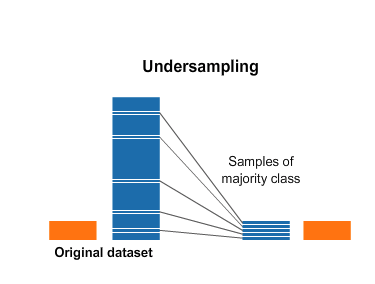
\includegraphics[width=.7\textwidth]{figures/Undersampling.png}
\caption{Undersampling Technique \cite{OverUnderIbm2019}}
\label{fig:undersampling}
\end{figure}

It involves removing samples from the dataset until the data
is balanced. The reasons to use under-sampling are usually related to practical 
reasons, such as resource costs. The techniques presented are:

\textbf{Undersampling} involves deleting samples from the majority class, with 
or 
without replacement. It is one of the early proposals to deal with imbalanced 
datasets. Although it may alleviate the imbalance in the dataset, it may also 
increase the variance of the classifier or discard meaningful samples from the 
majority class.

\textbf{Cluster Centroid} replaces a cluster of samples by the cluster centroid 
of a \textit{K-means} algorithm. The number of clusters is set by the level of 
undersampling.

\textbf{Near Miss}\label{nearmiss} refers to a collection of undersampling 
methods that select samples based on the distance of the majority class samples 
to the minority class samples~\cite{Zhang03}. There are three versions of this 
algorithm: 

\begin{enumerate}
	\item \textit{NearMiss-1} selects majority class samples with minimum 
	average distance to three closest minority class samples; 
	\item \textit{NearMiss-2} selects majority class examples with minimum 
	average distance to the three furthest minority class examples;
	\item \textit{NearMiss-3} selects majority class examples with minimum 
	distance to each minority class example.
\end{enumerate}

Among all the available techniques, \textit{Near Miss} has been the on used
for this research. Other techniques that remove instances intelligently include 
the Edited Nearest Neighbor (ENN) and Wilson's Editing that remove instances in 
which close neighbors belong to a  different class~\cite{wilson1972asymptotic}.

%%%%%%%%%%%%%%%%%%%%%%%%%%%%%%%%%%%%%%%%%%%%%%%%%%%%%%%%%%%%
\subsubsection{Oversampling}\label{sec:oversampling}

\begin{figure}[h!]
\centering
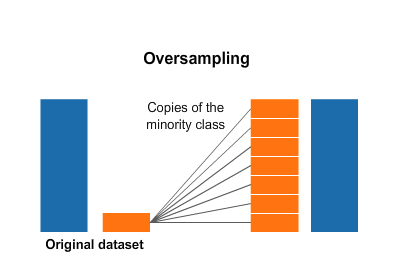
\includegraphics[width=.7\textwidth]{figures/Oversampling.png}
\caption{Oversampling Technique \cite{OverUnderIbm2019}}
\label{fig:oversampling}
\end{figure}

It involves replicating or creating new data points from the already 
existing data. The techniques analyzed are:

\textbf{Oversampling} involves copying supplementary data from the minority 
classes. It can be done more than once (actually, as many times as the 
developers sees fit). One of the early proposals regarding imbalanced datasets. 
It is robust, as it may randomly replace some of the samples from the minority 
class.

\textbf{SMOTE}\label{smote} (Synthetic Minority Oversampling 
Technique~\cite{ChawlaBHK02}) is one of the most popular oversampling techniques. 
It works by selecting samples close in the feature space. That means, that a 
line is drawn between the samples in the feature space and the a new sample at a
point along that line. It is effective because the samples from the minority 
class created are plausible - relatively close in feature space to existing 
samples from minority class. A downside of this technique is that samples are 
created without looking at the majority class, meaning a possible overlapping of 
classes.

\textbf{ADASYN} (ADaptative SYNthetic) sampling algorithm was developed using 
the SMOTE approach shifting the importance of the classification boundary to 
those minority classes which are difficult. It weights the most difficult to 
learn classes so that those have more importance when creating new data. In 
other words, ADASYN generates more synthetic data in the minority class samples 
that are harder to learn.

The technique selected for this article is the SMOTE method, implemented by the 
\textit{imbalance-learn}
\footnote{\url{https://imbalanced-learn.readthedocs.io/en/stable/}} Python 
package.

%%%%%%%%%%%%%%%%%%%%%%%%%%%%%%%%%%%%%%%%%%%%%%%%%%%%%%%%%%%%%%%%%%%
\subsection{Cost-Sensitive Classifiers}\label{subsec:costSensitive}

Also known as CSC. These are adapted classifiers that handle imbalanced 
datasets by either:

\begin{enumerate}
    \item Adding weights to instances\footnote{Can only be used if the base 
    classifier algorithm allows it}.
    \item Resampling the training data according to the costs assigned to each 
    class in a predefined cost matrix.
    \item Or generating a model that minimizes the expected cost\footnote{It can 
	be obtained by multiplying the predicted probability distribution with the 
	misclassification costs}. The idea behind this methodology is to penalize 
	differently each type of error - in the specific case of binary 
	classification, the false positives (FP) and false negatives (FN).
\end{enumerate}

The problem with CSC is defining the cost matrix as there is no systematic 
approach to do so. However, it is common practice to set the cost to equalize 
the class distribution.

%%%%%%%%%%%%%%%%%%%%%%%%%%%%%%%%%%%%%%%%%%%%%%%%%%%%%%%%%%%%%%%%%%%
\subsection{Ensembles}\label{sec:ensembles}

Also known as meta-learners are a combination of multiple models with the 
objective of obtaining better predictions. They are typically classified as 
\emph{Bagging}, \emph{Boosting} and \emph{\emph{Stacking}} - Stacked 
generalization.

%%%%%%%%%%%%%%%%%%%%%%%%%%%%%%%%%%%%%%%%%%%%%%%%%%%%%%%%%%%%

\textbf{Bagging}~\cite{Breiman96} (also known as Bootstrap aggregating) is a 
ensemble technique that involves a base learner applied to multiple equal size 
datasets. These datasets are created from the original data using bootstraping. 
Predictions are made on voting of the individual predictions. 

An advantage of this technique is that it does not require to modify
any aspect of the learning algorithm, taking advantage of the instability of 
the base classifier to create diversity among individual ensembles - so that 
individual members of the ensemble perform well in different regions of the 
data. However, if the output is robust to perturbation of the data (like is the 
case with nearest-neighbor -NN- classifiers) the performance drops and should 
not be used with those base classifiers.

%%%%%%%%%%%%%%%%%%%%%%%%%%%%%%%%%%%%%%%%%%%%%%%%%%%%%%%%%%%%

\textbf{Boosting} techniques generate multiple models that complement each 
other. The final objective is to induce models that improve certain regions of 
the data, where previous induced models had low performance. This can be 
achieved by increasing the weights of instances that have been wrongly 
classified. That way, new learners focus on those regions. 

Classification is based on a weighted voted among all members of the ensemble.
One of the most popular boosting algorithms is AdaBoost.M1~\cite{Freund1996} 
for classification. The set of training examples is assigned an equal weight at 
the beginning and the weight of instances can be increased or decreased 
depending on the classification of the learner. The next iterations focus on 
those instances with higher weights. AdaBoost.M1 can be applied to any base 
learner.

Models from ensembles are difficult to interpret (black-box behavior), 
comparing them to decision trees or rules providing explanation of their 
decision making process.

%%%%%%%%%%%%%%%%%%%%%%%%%%%%%%%%%%%%%%%%%%%%%%%%%%%%%%%%%%%%%%%%%%%%%%
\subsection{Hybrid Approaches}\label{subsec:hybridApproaches}

There are other hybrid approaches that can be used. Like that ones that
are going to be explained in the following section.

%%%%%%%%%%%%%%%%%%%%%%%%%%%%%%%%%%%%%%%%%%%%%%%%%%%%%%%%%%%%

\textbf{SMOTEBoost} tries to reduce the bias from the learning procedure due to 
the class imbalance, and increase the sampling weight for the minority class. 
SMOTE~\cite{CBHK2002} is introduced in each round of boosting, which enables 
each learner to be able to sample more of the minority class cases, and learn 
better and broader decision regions for the minority class. 

It also brings the benefit of enhancing the probability of selection for 
the difficult minority class cases that are dominated by the majority class 
points~\cite{CLHB2003}. The variation of boosting procedure of the SMOTEBoost 
process is a variant of the AdaBoost.M2 procedure~\cite{FS1997}.

%%%%%%%%%%%%%%%%%%%%%%%%%%%%%%%%%%%%%%%%%%%%%%%%%%%%%%%%%%%%

\textbf{RUSBoost}~\cite{Seiffert2010} uses the AdaBoost.M2. The difference with 
SMOTEBoost is that RUSBoost applies Random Under Sampling instead of SMOTE. The 
application of SMOTE at this point has two drawbacks that 
RUSBoost is designed to overcome:

\begin{itemize}
    \item It increases the complexity of the algorithm. SMOTE finds the $k$ 
    nearest neighbors of the minority class samples, and then extrapolates
    them to make new synthetic samples. RUS, on the other hand, simply deletes 
	the majority class examples randomly.

    \item RUS produces less training data (as it is an undersampling 
    technique, not like SMOTE, which is an oversampling technique). This can
    be translated into shorter model training times~\cite{Seiffert2010}.
\end{itemize}

%%%%%%%%%%%%%%%%%%%%%%%%%%%%%%%%%%%%%%%%%%%%%%%%%%%%%%%%%%%%

\textbf{MetaCost}~\cite{Domingos1999} is a combination of bagging with 
cost-sensitive classification. The bagging part of the technique is used to 
relabel training data so that each training example is assigned a prediction 
that minimizes the expected cost for that instance. Based on the modified 
training data, MetaCost induces a new classifier which provides information 
about how a decision was reached.

%%%%%%%%%%%%%%%%%%%%%%%%%%%%%%%%%%%%%%%%%%%%%%%%%%%%%%%%%%%%%%%%%%%%%%
\subsection{Defect Prediction}\label{subsec:defectPrediction}

Regarding the problem of software defect prediction, many techniques have been 
proposed in the literature - statistical methods (regression~\cite{Bibi2008}, 
and Support Vector Machines~\cite{Elish2008}, etc.), machine learning 
(classification trees~\cite{Khoshgoftaar02}), neural 
networks~\cite{Khoshgoftaar97}), probabilistic models 
(Na\"ive Bayes~\cite{Menzies07b} and Bayesian networks), ensembles of different 
techniques and meta-heuristics (ant colonies~\cite{Vandecruys2008}, etc). 
Despite this fact, some discrepancies are found:

\begin{itemize}
    \item No classifier is consistently better than others.
    \item There is no optimum metric that allows the evaluation and comparison
    of classifiers (\cite{Mende09,Zhang07,Menzies07b}).
    \item Data is also affected by quality issues - class imbalance, 
    overlapping, outliers, etc..
\end{itemize}

Some authors highlight the problem of imbalanced datasets when dealing with
the project at hand, defect prediction (Seiffert et al.~\cite{Seiffert2009} and 
in Khoshgoftaar et al.~\cite{Khoshgoftaar03}).

As it has been mentioned before, there is no classifier that behaves 
consistently better. No technique is able to give a an outstanding performance 
when evaluating classifiers. Some authors have compared performance of several 
measures (e.g., Peng~\cite{Peng2009}, Peng et al.~\cite{Peng2010}, this paper 
actually propose performance metrics to evaluate merit of classification 
algorithms and ranked classification algorithms, respectively).

Further analysis on the subject comes from the hand of Lessman et 
al.~\cite{LBMP08}. This paper compared several classifiers, discussing 
performance metrics such like $TP_r$ and $FP_r$. But finally advocated to use 
the AUC\footnote{Further explained in Section~\ref{sec:roc}, Area Under the ROC 
Curve} as a good indicator for classifiers comparison. This results is known as 
sub-optimal for highly imbalanced datasets.

Arisholm et al.~\cite{ARISHOLM20102} compared different classification
algorithms (tree algorithm (C4.5), coverage rule algorithm (PART), logistic 
regression, back-propagation neural networks and Support Vector Machines) over 
13 different Java developed systems. They used three metrics to compare results:

\begin{itemize}
    \item Object-oriented metrics.
    \item Churn ($\delta$) metrics between successive releases.
    \item Process management metrics from a configuration management system.
\end{itemize}

The conclusion was that large differences can be achieved depending on the 
comparison criteria of the data. To solve this problem, the paper proposed a 
new AUC based, cost-effectiveness metric. Same approach has been evaluated and 
explored in Mende and Koschke~\cite{Mende10}.


%%%%%%%%%%%%%%%%%%%%%%%%%%%%%%%%%%%%%%%%%%%%%%%%%%%%%%%%%%%%%%%%%%%%%%%%%%%
%
% Generic template for TFC/TFM/TFG/Tesis
%
% $Id: introduccion.tex,v 1.19 2015/02/24 23:21:54 macias Exp $
%
% By:
%  + Javier Macías-Guarasa. 
%    Departamento de Electrónica
%    Universidad de Alcalá
%  + Roberto Barra-Chicote. 
%    Departamento de Ingeniería Electrónica
%    Universidad Politécnica de Madrid   
% 
% Based on original sources by Roberto Barra, Manuel Ocaña, Jesús Nuevo,
% Pedro Revenga, Fernando Herránz and Noelia Hernández. Thanks a lot to
% all of them, and to the many anonymous contributors found (thanks to
% google) that provided help in setting all this up.
%
% See also the additionalContributors.txt file to check the name of
% additional contributors to this work.
%
% If you think you can add pieces of relevant/useful examples,
% improvements, please contact us at (macias@depeca.uah.es)
%
% Copyleft 2013
%
%%%%%%%%%%%%%%%%%%%%%%%%%%%%%%%%%%%%%%%%%%%%%%%%%%%%%%%%%%%%%%%%%%%%%%%%%%%

\chapter{Empirical Work}\label{chp:empwork}

In this chapter, we cover the experimental work carried out. Firstly, we 
describe the datasets used for the experimentation; then, the supervised 
classifiers evaluated; the evaluation metrics chosen; and finally, present and 
discuss the results.

%%%%%%%%%%%%%%%%%%%%%%%%%%%%%%%%%%%%%%%%%%%%%%%%%%%%%%%%%%%%%%%%%%%%%%%%%%%%%%%%
\section{Datasets}\label{sec:datasets}

In this work, publicly available datasets in the domain of Software defect 
prediction were used, were used, the Jureczko and Madeyski dataset
\footnote{\url{http://snow.iiar.pwr.wroc.pl:8080/MetricsRepo/}} 
\cite{Jureczko2010, MadeyskiJ2015}, the Apache dataset 
(\cite{Zimmermann07Eclipse}) and the Harman Search Base dataset 
\cite{Harman2014ssbse}. 

From the first cluster of datasets, 15 open source projects are the ones chosen 
(a total of 8 are used for this project). The number of defects found in each 
class collected from the Software Management System (SCM) using a regular 
expression. The datasets are publicly available  (can be found in the PROMISE 
repository~\cite{promiserepo}). These datasets have been used in previous 
researches, \cite{Xu2018, Wang2016, Xia2016}, which allows comparing and 
analyzing the obtained results.

A sample can be considered as \textit{defective} when the number of defects 
inside the class is more than 0. Similarly, if the number of defects is 0, then 
the class is \textit{non-defective}. This allows a binary classification, making 
easier handling results, operations and comparisons.

\begin{center}
\begin{longtable}{ | l | l | }
\caption{Defect Metrics Dataset Variables}\label{tab:dataJureczkoMetrics} \\

\hline
 \emph{Metric} & \emph{Description} \\
\hline 
\hline
\endfirsthead
\multicolumn{2}{c}{\tablename\ \thetable\ -- \textit{Continued from previous page}} \\
\hline
\emph{Metric} & \emph{Description} \\
\hline 
\hline
\endhead
\hline
\multicolumn{2}{r}{\textit{Continued on next page}}
\endfoot
\hline
\endlastfoot
WMC    &    Weighted methods per class \cite{Chidamber1994} \\
DIT    &    Depth of Inheritance Tree \cite{Chidamber1994} \\
NOC    &    Number of Children \cite{Chidamber1994} \\
CBO    &    Coupling between object classes \cite{Chidamber1994} \\
RFC    &    Response for a Class \cite{Chidamber1994} \\
LCOM   &    Lack of cohesion in methods \cite{Chidamber1994} \\
Ca     &    Afferent couplings \cite{Martin1994} \\
Ce     &    Efferent couplings \cite{Martin1994} \\
NPM    &    Number of Public Methods \cite{Bansiya2002} \\
LCOM3  &    Lack of cohesion in methods \cite{Henderson-Sellers1995} \\
LOC    &    Lines of Code \cite{Bansiya2002} \\
DAM    &    Data Access Metric \cite{Bansiya2002} \\
MOA    &    Measure of Aggregation \cite{Bansiya2002} \\
MFA    &    Measure of Functional Abstraction \cite{Bansiya2002} \\
CAM    &    Cohesion Among Methods of Class \cite{Bansiya2002} \\
IC     &    Inheritance Coupling \cite{Tang} \\
CBM    &    Coupling Between Methods \cite{Tang} \\
AMC    &    Average Method Complexity \cite{Tang} \\
MAX\textunderscore CC    &    Maximum McCabe's cyclomatic complexity \cite{McCabe1976} \\
AVG\textunderscore CC    &    Average McCabe's cyclomatic complexity \cite{McCabe1976} \\
\hline
\end{longtable}
\end{center}

There is another sole dataset obtained from the same source as the previous 
collection of datasets, with a very similar structure of data, the 
\textit{Apache} dataset. It has the same origin and objective as its 
predecessors.

On the second cluster of datasets, the data comes from a total of 8 different 
Hadoop versions. Their original purpose is to train a search based fault 
prediction system. 

Similarly to Jureczko and Madeyski dataset \cite{Jureczko2010, MadeyskiJ2015}, 
it uses: (1) WMC, (2) DIT, (3), NOC, (4) CBO, (5) RFC, (6) LCOM, (7) NOM, and 
(8) LOC; metrics to define each dataset.

Regarding more information on the content of the datasets the next table (see 
Table~\ref{tab:metrics-description}) summarizes the number of samples on each 
dataset and further valuable information, such as the absolute and relative 
number of defects for those datasets.

\begin{center}
\begin{longtable}{ | c | c | c c c c | }
\caption{Description of the Datasets} \label{tab:metrics-description} \\

\hline
\emph{Project} & \emph{Version} & 
\emph{\#instances} & \emph{\#Non-Defective} & \emph{\#Defective} & \emph{\%Defective} \\
\hline 
\hline
\endfirsthead
\multicolumn{6}{c}{\tablename\ \thetable\ -- \textit{Continued from previous page}} \\
\hline
\emph{Project} & \emph{Version} & 
\emph{\#instances} & \emph{\#Non-Def} & \emph{\#Def} & \emph{\%Def} \\
\hline
\hline
\endhead
\hline
\multicolumn{6}{r}{\textit{Continued on next page}}
\endfoot
\hline
\endlastfoot

\multirow{5}{*}{ant} &  
    1.3 &   125 &   105 &    20 &   16.00 \\
&   1.4 &   178 &   138 &    40 &   22.47 \\ 
&   1.5 &   293 &   261 &    32 &   10.92 \\
&   1.6 &   351 &   259 &    92 &   26.21 \\
&   1.7 &   745 &   579 &   166 &   22.28 \\

\hline
\multirow{1}{*}{apache} &  
    -   &   191 &   107 &   84  &   43.98 \\

\hline
\multirow{4}{*}{camel} &   
    1.0 &   339 &   326 &    13 &    3.83 \\
&   1.2 &   608 &   392 &   216 &   35.52 \\
&   1.4 &   872 &   727 &   145 &   16.62 \\
&   1.6 &   965 &   777 &   188 &   19.48 \\

\hline
\multirow{8}{*}{hadoop} &
    0.1 &   141 &    91 &    50 &   35.60 \\
&   0.2 &   191 &   149 &    42 &   21.99 \\
&   0.3 &   211 &   158 &    53 &   25.12 \\
&   0.4 &   201 &   159 &    42 &   20.90 \\
&   0.5 &   217 &   180 &    37 &   17.05 \\
&   0.6 &   234 &   203 &    31 &   13.25 \\
&   0.7 &   250 &   202 &    48 &   19.20 \\
&   0.8 &   240 &   224 &    16 &    6.67 \\

\hline
\multirow{2}{*}{ivy} &   
    1.4 &   241 &   225 &    16 &    6.63 \\
&   2.0 &   352 &   312 &    40 &   11.36 \\

\hline
\multirow{5}{*}{jedit} & 
    3.2 &   272 &   182 &    90 &   33.08 \\
&   4.0 &   306 &   231 &    75 &   24.50 \\
&   4.1 &   312 &   233 &    79 &   25.32 \\
&   4.2 &   367 &   319 &    48 &   13.07 \\
&   4.3 &   492 &   481 &    11 &    2.23 \\

\hline
\multirow{3}{*}{log4j} & 
    1.0 &   135 &   101 &    34 &   25.18 \\
&   1.1 &   109 &    72 &    37 &   33.94 \\
&   1.2 &   205 &    16 &   189 &   92.19 \\

\hline
\multirow{3}{*}{synapse} &
    1.0 &   157 &   141 &    16 &   10.19 \\
&   1.1 &   222 &   162 &    60 &   27.02 \\
&   1.2 &   256 &   170 &    86 &   33.59 \\

\hline
\multirow{4}{*}{xalan} & 
    2.4 &   723 &   613 &   110 &   15.21 \\
&   2.5 &   803 &   416 &   387 &   48.19 \\
&   2.6 &   885 &   474 &   411 &   46.44 \\
&   2.7 &   909 &    11 &   898 &   98.78 \\

\hline
\multirow{3}{*}{xerces} &
    1.2 &   440 &   369 &    71 &   16.13 \\
&   1.3 &   453 &   384 &    69 &   15.23 \\
&   1.4 &   588 &   151 &   437 &   74.31 \\
\hline

\end{longtable}
\end{center}

The experiments of this paper use the latest version of the datasets 
\textit{ant}, \textit{apache}, \textit{camel}, \textit{hadoop}, \textit{ivy},
\textit{jedit}, \textit{log4j}, \textit{xalan} and \textit{xerces}; alongide
all the available versions of the \textit{hadoop} dataset.

%%%%%%%%%%%%%%%%%%%%%%%%%%%%%%%%%%%%%%%%%%%%%%%%%%%%%%%%%%%%%%%%%%%%%%%%%%%%%%%%
\section{Supervised Classifiers}

This work makes use of several supervised learning algorithms. The 
experiments carried out use the following algorithms:

\begin{description}
    \item [Naive Bayes] (NB)~\cite{Mit97} is a classifier that works on 
	conditional probabilities, uses the Bayes theorem to predict the class for 
	each data input. Calculates the probability of a certain event, given prior 
	knowledge. This classifier assigns a set of attributes $a_{1}, \ldots, 
	a_{n}$ to a given class $C$ so that the probability of the class description 
	value of the attributes instances is maximal: $P(C|a_{1}, \ldots, a_n)$. The 
	probability of the hypothesis, given that the evidence is true, is the 
	probability of the evidence, given the hypothesis is true, multiplied by the 
	probability of the hypothesis; in relation to the probability of the 
	evidence. See Eq.~\ref{eq:bayes}.
    
    \begin{equation}\label{eq:bayes}
        P(H|E) = \frac{(E|H) * P(H)}{P(E)}
    \end{equation}
    
    For this project it has been selected the Gaussian Naive Bayes from 
	\texttt{scikit-learn}
	\footnote{\url{https://scikit-learn.org/stable/modules/generated/sklearn.naive_bayes.GaussianNB.html}} 
	to perform the experimentation. Being \textit{Gaussian} means that the 
	likelihood of the features is assumed to be Gaussian. The formula is given 
	by Eq.~\ref{eq:gaussian}.
    
    \begin{equation}\label{eq:gaussian}
        P(x_{i}|y)=(\frac{1}{\sqrt{2\pi \sigma^{2}_{y}}})\exp{(-\frac{(x_{i} - \mu _{y})^2}{2\sigma^{2}_{y}})}
    \end{equation}
    
    \item [Decision Trees] can be seen as rules with a root node, branches are 
	conditions and leaves correspond to classes. There are many decision trees 
	algorithm such as CART (Classification And Regression 
	Trees)~\cite{Breiman1984} is a non-parametric decision tree, similar to 
	\textbf{C4.5}~\cite{Quinlan1993}. 

	CART constructs a two branch bifurcation of the most discriminating 
	attribute, based on the Gini index. It can generate either classification or 
	regression trees - depends on the variable (categorical or numeric, 
	respectively). The implementation available in 
	\texttt{scikit-learn}~\cite{scikit-learn}
	\footnote{\url{https://scikit-learn.org/stable/modules/tree.html}} is an 
	optimised version of this algorithm, although it does not support 
	categorical variables.
    
    \item [Nearest Centroid] classifier\cite{conformal2014},  \textbf{Nearest 
	Prototype} classifier, or \textbf{Rocchio classifier} for its similarity to 
	an algorithm with the same name (see Eq.\ref{eq:rocchio}). 
    
    \begin{equation}\label{eq:rocchio}
        \overrightarrow{Q_{m}} =  (a \cdot \overrightarrow{Q_{o}}) + (b \cdot 
        \frac{1}{\lvert D_{r} \rvert} \cdot \sum_{\overrightarrow{D_{j}} \in 
        D_{r}} \overrightarrow{D_{j}}) - (c \cdot \frac{1}{\lvert D_{nr} 
        \rvert} \cdot \sum_{\overrightarrow{D_{k}} \in D_{nr}} 
        \overrightarrow{D_{k}})
    \end{equation}
    
    The labels of a given sample are assigned by evaluating the classes of 
	training samples whose mean is closest to the evaluated point. The training 
	procedure, given a labeled training set ${(\overrightarrow{x_{1}}, y_{1}), 
	\ldots,  (\overrightarrow{x_{n}}, y_{n})}$ with class labels $y_{i} \in Y$, 
	compute the per-class centroid with Eq.~\ref{eq:knntrain}.
    
    \begin{equation}\label{eq:knntrain}
        \overrightarrow{\mu _{l}} = \frac{1}{\lvert C_{l} \rvert} \sum_{i \in 
        C_{l}} \overrightarrow{x_{i}}
    \end{equation}
    
    \noindent where $C_{l}$ is the set of indices of samples belonging to class 
	$l \in Y$.  The prediction functions, takes the class assigned to an 
	observation $\overrightarrow{x}$ is Eq.~\ref{eq:knnpred}.
    
    \begin{equation}\label{eq:knnpred}
        \overrightarrow{y} = argmin_{l \in Y} \lvert\lvert \overrightarrow{\mu _{l}} - \overrightarrow{x} \rvert\rvert
    \end{equation}

\end{description}

%%%%%%%%%%%%%%%%%%%%%%%%%%%%%%%%%%%%%%%%%%%%%%%%%%%%%%%%%%%%%%%%%%%%%%%%%%%%%%%%
\section{Evaluation Metrics}\label{sec:ev-metrics}

Part of the process of applying a classification algorithm is to measure the 
success and the results of the training. In order to do it, some metrics can be 
calculated out of the testing to the trained classifier. Here is where the
Confusion Matrix comes at hand. The Confusion Matrix (see 
Table~\ref{tab:conf-matrix}) allows us to summarize the performance of a given 
classification algorithm, it is also the foundation of many of the performance 
metrics used in classification by:

% --> Confusion Matrix
\begin{table}[h!]
\centering
\footnotesize
\caption{Confusion Matrix for Binary Classification}
\label{tab:conf-matrix}
\begin{tabular}{c c | p{2.5cm} | p{2.5cm} }
% ROW1
  & & \multicolumn{2}{c}{\emph{Actual Class}}\\
% ROW2
  & &    \emph{Positive} & \emph{Negative} \\
% ROW3
  \hline
  \multirow{4}{*}{\emph{Predicted Class}}
  &\emph{Positive} & True Positive \newline ($TP$) & False Positive \newline ($FP$)\\
% ROW 4
  %\hline
  \cline{2-4}
  &\emph{Negative} & False Negative \newline ($FN$) & True Negative\newline ($TN$)\\
\end{tabular}
\end{table}

\begin{description}
 \item [True Positive (TP)] - Data is correctly classified as positive.
 \item [True Negative (TN)] - Data is correctly classified as negative.
 \item [False Positive (FP)] - Data being negative classified as positive.
 \item [False Negative (FN)] - Data being positive classified as negative. 
\end{description} 

These specifications indicate that the input data should have a binary target: 
one value that can be classified as \textit{positive} and a second value that 
can be classified as negative. From this statistical classification
\footnote{Also know as error matrix.}, many performance measures can be 
calculated. Some of the most widely used metrics, and the ones used in this 
paper are explained next.

%%%%%%%%%%%%%%%%%%%%%%%%%%%%%%%%%%%%%%%%%%%%%%%%%%%%%%%%%%%%%%%%%%%%%%
\subsection{Precision}    
 
Also know as Positive Predictive Value (PPV). It is the relation 
between the \textit{true positives} calculated and the overall positives 
detected by the classification algorithm (see Eq.~\ref{eq:ppv}).
 
\begin{equation}\label{eq:ppv}
    PPV = \frac{TP}{TP + FP} = 1 - FDR
\end{equation}

%%%%%%%%%%%%%%%%%%%%%%%%%%%%%%%%%%%%%%%%%%%%%%%%%%%%%%%%%%%%%%%%%%%%%%
\subsection{Recall} 

Also known as sensitivity, hit rate, or True Positive 
Rate (TPR). It stands for the relation between the \textit{true positives} 
calculated and the real number of positives (see Eq.~\ref{eq:tpr}).

\begin{equation}\label{eq:tpr}
    TPR = \frac{TP}{P} = \frac{TP}{TP + FN} = 1 - FNR
\end{equation}

%%%%%%%%%%%%%%%%%%%%%%%%%%%%%%%%%%%%%%%%%%%%%%%%%%%%%%%%%%%%%%%%%%%%%%
\subsection{Fall-out}

Also called False Positive Rate (FPR). It is the probability of rejecting 
(falsely) the null hypothesis\footnote{General statement or default position
that there is no relationship between two measured phenomena or no
association among groups.} for a particular test (see Eq.~\ref{eq:fpr}).

\begin{equation}\label{eq:fpr}
    FPR = \frac{FP}{N} = \frac{FP}{FP + TN} = 1 - TNR
\end{equation}
    
%%%%%%%%%%%%%%%%%%%%%%%%%%%%%%%%%%%%%%%%%%%%%%%%%%%%%%%%%%%%%%%%%%%%%%
\subsection{Balance Accuracy}

It goes by the acronym BA. It is a metric generally used to evaluate how
good is a (binary) classifier. It is a measure that comes in specially 
handy for imbalanced datasets. Its formula is represented by the mean of
\textit{sensitivity} and \textit{specificity} (see Eq.~\ref{eq:ba}).

\begin{equation}\label{eq:ba}
    BA = \frac{TPR + TNR}{2}
\end{equation}
    
%%%%%%%%%%%%%%%%%%%%%%%%%%%%%%%%%%%%%%%%%%%%%%%%%%%%%%%%%%%%%%%%%%%%%%
\subsection{F-Measure} 
 
Also known as $F_1$, or \textit{S\o rensen-Dice coefficient} (independently 
developed by S\o rensen~\cite{sorensen1948} and Dice~\cite{dice1945}) is the 
harmonic mean of precision and sensitivity, the two previous measures, which 
measures accuracy (see Eq.~\ref{eq:f1}). It is twice the relation of the 
multiplication between \textit{recall} and \textit{precision} and their 
addition. It is commonly used in highly imbalanced datasets but there are also 
some criticisms as it does not take into account the \textit{True Negative} 
(\textit{TN}) cases.

\begin{equation}\label{eq:f1}
    F_1 = 2 \cdot \frac{PPV \cdot TPR}{PPV + TPR} = \frac{2 \cdot TP}{2 \cdot TP + FP + FN}
\end{equation}
    
%%%%%%%%%%%%%%%%%%%%%%%%%%%%%%%%%%%%%%%%%%%%%%%%%%%%%%%%%%%%%%%%%%%%%%    
\subsection{MCC} 

The Matthews Correlation Coefficient (MCC)~\cite{Matthews1975} or \textit{phi} 
coefficient measures the quality of a binary classification robust to the 
imbalance problem (Eq.~\ref{eq:mcc}). Its range values are between -1 and +1, 
where -1 represents complete inconsistency (disagreement), 0 indicates that the 
prediction is no better than a random prediction; and +1 would be a perfect 
prediction.  

\begin{equation}\label{eq:mcc}
    MCC = \frac{TP \cdot TN - FP \cdot FN}{\sqrt{(TP + FP)(TP + FN)(TN + FP)(TN + FN)}}
\end{equation}

%%%%%%%%%%%%%%%%%%%%%%%%%%%%%%%%%%%%%%%%%%%%%%%%%%%%%%%%%%%%%%%%%%%%%%
\subsection{Receiver Operating Characteristic Curve}\label{sec:roc}

The Receiver Operating Characteristic (ROC)\cite{Fawcett2006} Curve represents 
graphically the True Positive Rate (TPR) versus the False Positive Rate (FPR) as 
shown in Figure~\ref{fig:roc}.

\begin{figure}
\centering
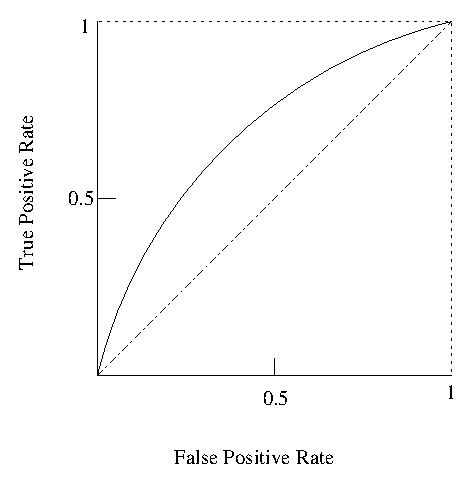
\includegraphics[width=.4\textwidth]{roc} % width=9cm, height=6cm
\caption{ROC Curve}
\label{fig:roc}
\end{figure}

Once the curve is plotted, the more the curve gets similar to a slope of 
$TPR = FPR$ the more imbalance that can be found in the dataset. It provides
graphical visualization of the results. 

The Area Under the ROC Curve (AUC) is a quality measure between positive and 
negative rates with a single value. This metric allows to compare models.

An approximation to the function can be calculated with Eq~\ref{eq:auc}.

\begin{equation}\label{eq:auc}
    AUC = \frac{1 + TP_{r} - FP_{r}}{2}
\end{equation}


Typically, three unbiased metrics, i.e., AUC, F-score 
(\cite{sorensen1948,dice1945}), Matthews Correlation Coefficient 
(MCC - \cite{Matthews1975}), are used to evaluate the performance on imbalanced 
datasets. Other measures cannot be used when data is highly imbalanced, like 
\textit{accuracy} (\textit{Acc}) (defined by Eq.~\ref{eq:accuracy}), as it does 
not take into account the number of labels of different classes.

\begin{equation}\label{eq:accuracy}
    Acc = \frac{TP + TN}{TP + TN + FP + FN}
\end{equation}

%%%%%%%%%%%%%%%%%%%%%%%%%%%%%%%%%%%%%%%%%%%%%%%%%%%%%%%%%%%%%%%%%%%%%%%%%%%%%%%%
\section{Results and discussion}

%%%%%%%%%%%%%%%%%%%%%%%%%%%%%%%%%%%%%%%%%%%%%%%%%%%%%%%%%%%%%%%%%%%%%%

\subsection{Methodology}

To answer the research questions stated in Section \ref{sec:aim-obj}, we run 
several experiments. First, we analyse the complexity metrics (see 
Section~\ref{sec:ecol}) from all selected datasets (see 
Section~\ref{sec:datasets}). Then, we retrieve some analytical metrics (see 
Section~\ref{sec:ev-metrics}), applying $K$-fold Cross
Validation to those datasets. Finally, we repeat the process applying some 
under/oversampling techniques with $K$-CV (see 
Sections~\ref{sec:undersampling} and~\ref{sec:oversampling}, respectively).

As the final aim is to see how complexity metrics affect classification and 
therefore the analytical metrics, a final section is going to summarize the 
results obtained and the conclusions drawn out of those measures and answer the 
research questions.

%%%%%%%%%%%%%%%%%%%%%%%%%%%%%%%%%%%%%%%%%%%%%%%%%%%%%%%%%%%%%%%%%%%%%%
\subsection{Data Complexity Metrics Analysis}

As it has been mentioned in \textit{Data Complexity Metrics} (see 
Section ~\ref{sec:ecol}), the software package to calculate them is 
available in R, 
\texttt{ECoL}\footnote{\url{https://github.com/lpfgarcia/ECoL/}}. Therefore, it
was necessary to call it from the Python environment. In order to do so, the 
package \texttt{RServe}, a client server implementation for R workspace to 
execute functions from other environments like Python, was used. In other words, 
this is a connector that allow us to execute the \texttt{ECoL} complexity
metrics functions. The source code regarding this connector can be found in the 
Appendix~\ref{chp:pythoncode}, Section~\ref{sec:rconnect}.

The rest of the experimental work was implemented in a Python script. 
The structure of the script tries to find and compare the complexity metrics 
obtained from different datasets to see if there is a certain relation between 
metrics. To do so, a script was developed (see 
Algorithm~\ref{alg:complexmetrics}) to connect Python to the ECoL library in R 
and returns the complexity metrics of a certain dataset (see its full 
implementation in Appendix~\ref{chp:pythoncode}, 
Section~\ref{sec:exp-kfold-code}).

\begin{breakablealgorithm}
    \caption{Datasets Complexity Metrics Comparison}
    \footnotesize
    \label{alg:complexmetrics}
    \begin{algorithmic}[1]
        \Require $\mathcal{D}$ dataset
        \Ensure $\mathcal{C}$ complexity metrics
        \State con $\leftarrow$ connectEcol()
        
        \ForAll {set in $\mathcal{D}$}
        	\State inputs, targets $\leftarrow$ getDataset(set)
        	
        	\State metrics $\leftarrow$ con.getMetrics(inputs, targets)
        	
        	\State $\mathcal{C}$.add(metrics)
        \EndFor
        
    \State plotComparison($\mathcal{C}$)
    \end{algorithmic}
\end{breakablealgorithm}

The results are also stored in CSV files, which are represented
as Tables~\ref{tab:complMetricsWholeDatasets_PROMISE} 
and~\ref{tab:complMetricsWholeDatasets_PROMISE2}.

The experiment has been repeated for two independents sets of 
datasets (see Section~\ref{sec:datasets} for more details regarding
the datasets and their content). The first experiment results are
summarized in Table~\ref{tab:complMetricsWholeDatasets_PROMISE}, whereas the 
second experiment, regarding the Hadoop datasets is shown in 
Table~\ref{tab:complMetricsWholeDatasets_PROMISE2}.

The obtained results are also showed in the following Figures: 
(\ref{fig:balance}) balance, (\ref{fig:correlation}) correlation, 
(\ref{fig:dimensionality}) dimensionality, (\ref{fig:linearity}) linearity, 
(\ref{fig:neighborhood}) neighborhood, (\ref{fig:network}) network, 
(\ref{fig:overlap}) overlap, and (\ref{fig:smoothness}) smoothness.

%%%%%%%%%%
\begin{figure}[h!]
    \centering
    \begin{subfigure}{0.496\textwidth}
        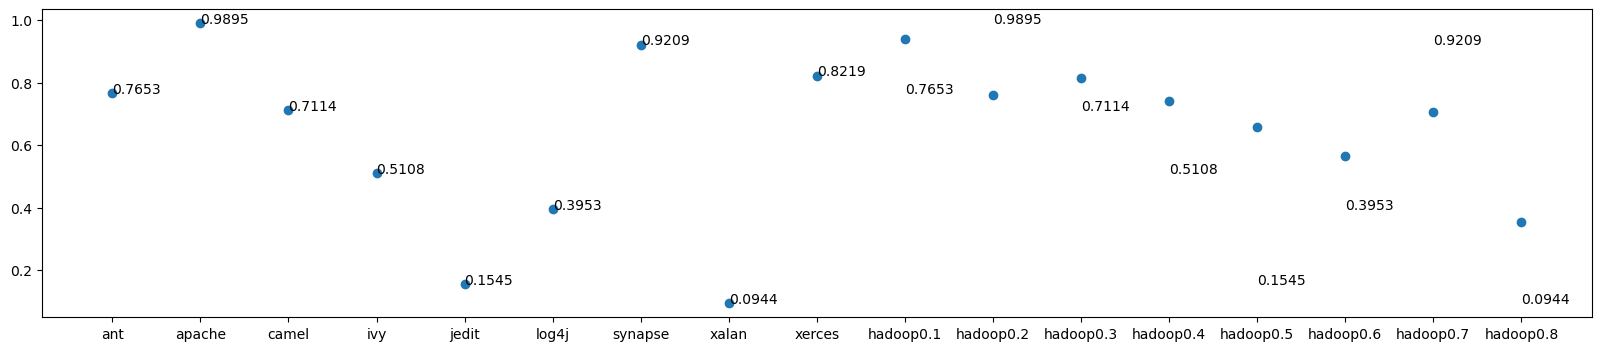
\includegraphics[width=0.99\linewidth]{figures/balance-C1.png}
        \caption{Balance C1}
        \label{fig:balance-c1}
    \end{subfigure}
    \begin{subfigure}{0.496\textwidth}
        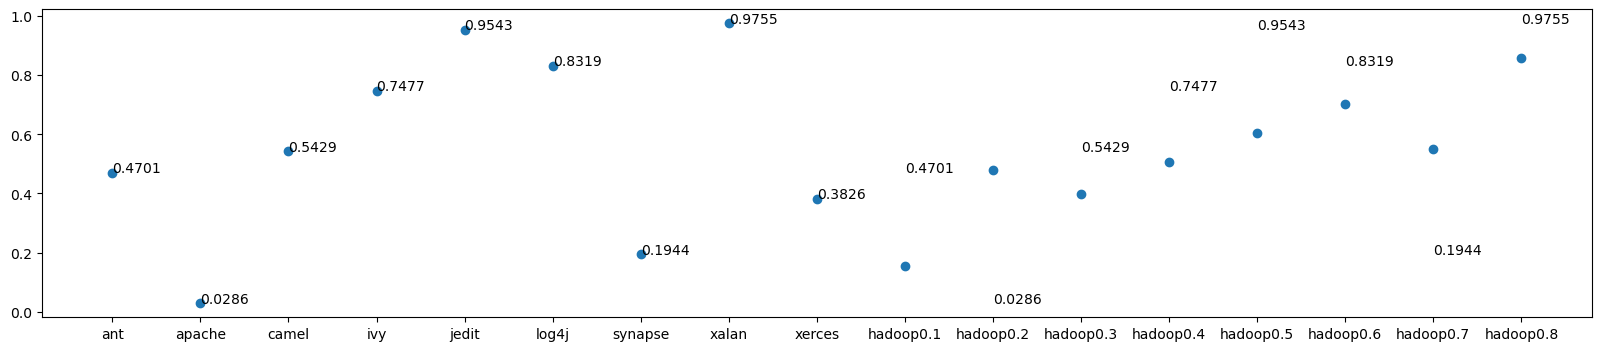
\includegraphics[width=0.99\linewidth]{figures/balance-C2.png}
        \caption{Balance C2}
        \label{fig:balance-c2}
    \end{subfigure}
    \caption{Balance Measures}
    \label{fig:balance}
\end{figure}

%%%%%%%%%%
\begin{figure}[h!]
    \centering
    \begin{subfigure}{0.496\textwidth}
        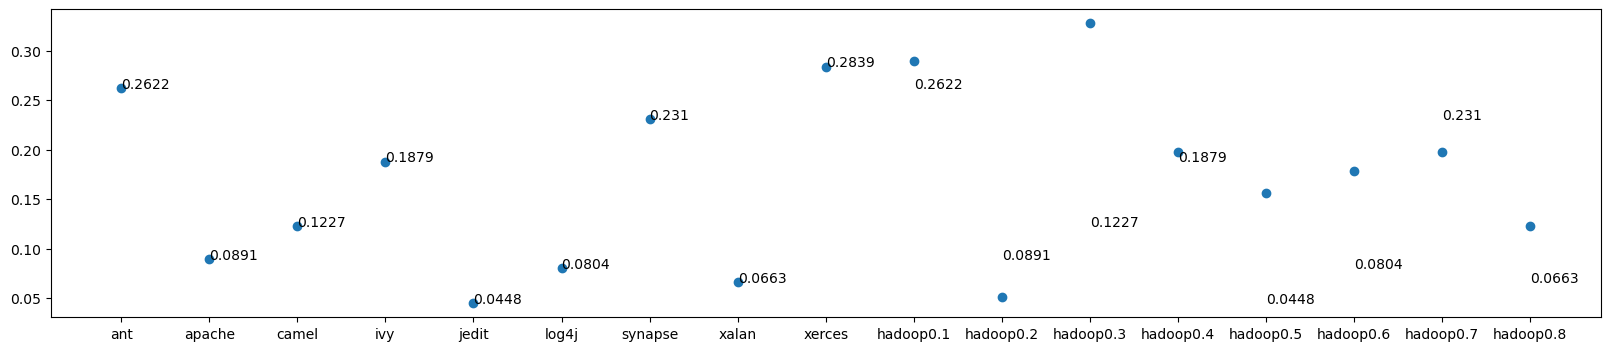
\includegraphics[width=0.99\textwidth]{figures/correlation-C2.png}
        \caption{Correlation C2}
        \label{fig:correlation-c2}
    \end{subfigure}
    \begin{subfigure}{0.496\textwidth}
        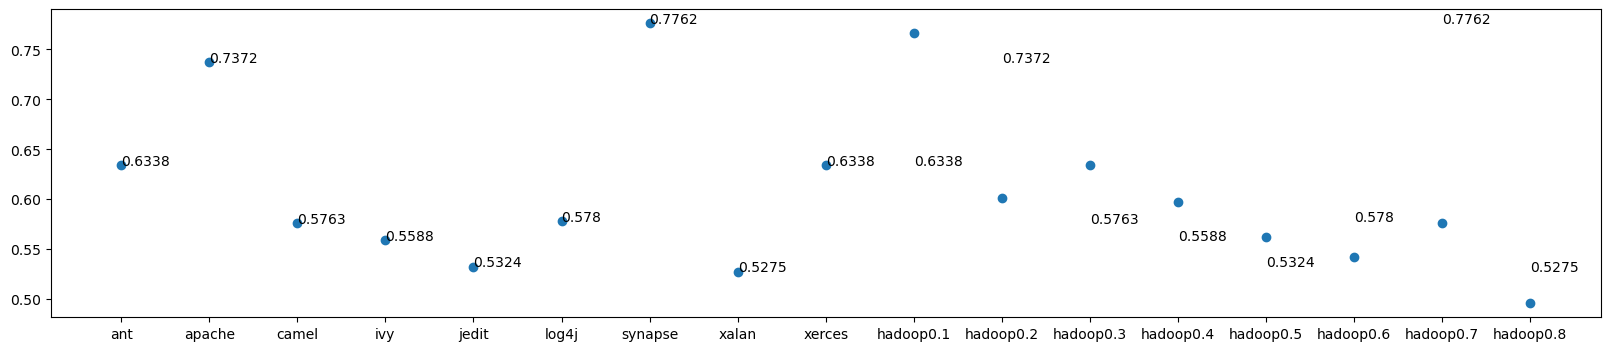
\includegraphics[width=0.99\textwidth]{figures/correlation-C3.png}
        \caption{Correlation C3}
        \label{fig:correlation-c3}
    \end{subfigure}
\end{figure}
\begin{figure}[h!]\ContinuedFloat
    \centering
    \begin{subfigure}{0.496\textwidth}
        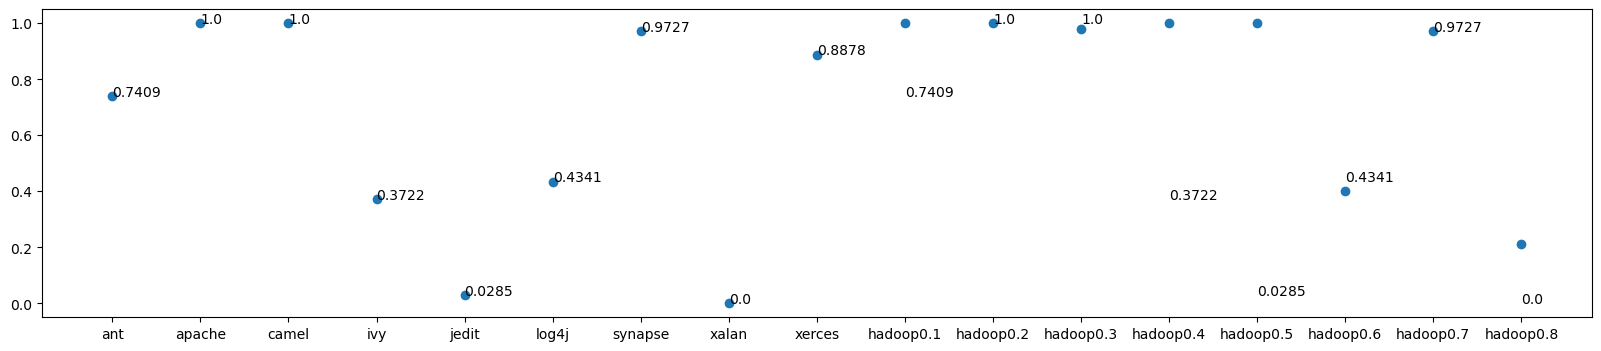
\includegraphics[width=0.99\textwidth]{figures/correlation-C4.png}
        \caption{Correlation C4}
        \label{fig:correlation-c4}
    \end{subfigure}
    \caption{Correlation Measures}
    \label{fig:correlation}
\end{figure}

%%%%%%%%%%
\begin{figure}[h!]
    \centering
    \begin{subfigure}{0.496\textwidth}
        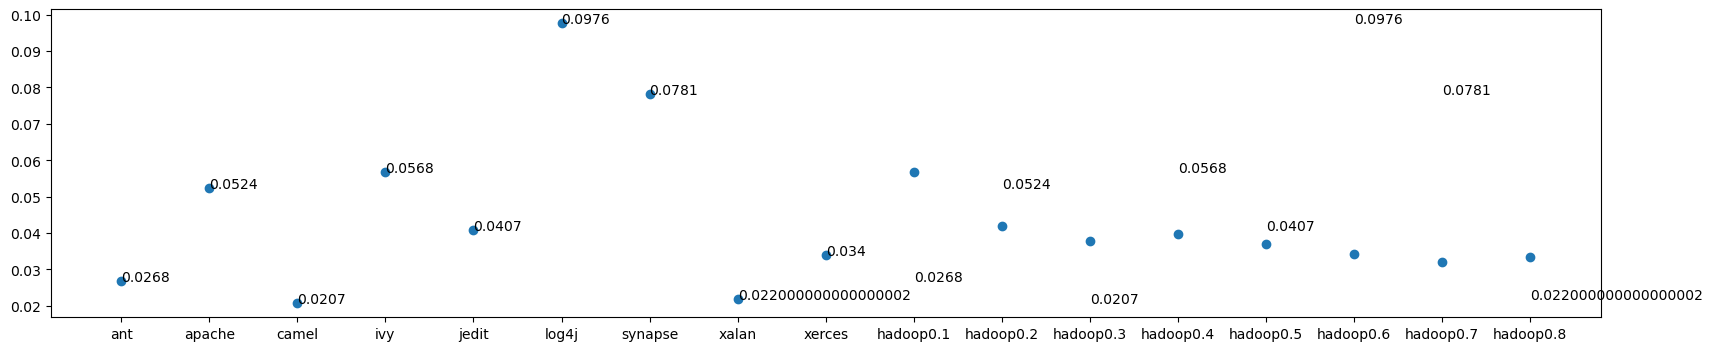
\includegraphics[width=0.99\textwidth]{figures/dimensionality-T2.png}
        \caption{Dimensionality T2}
        \label{fig:dimensionality-t2}
    \end{subfigure}
    \begin{subfigure}{0.496\textwidth}
        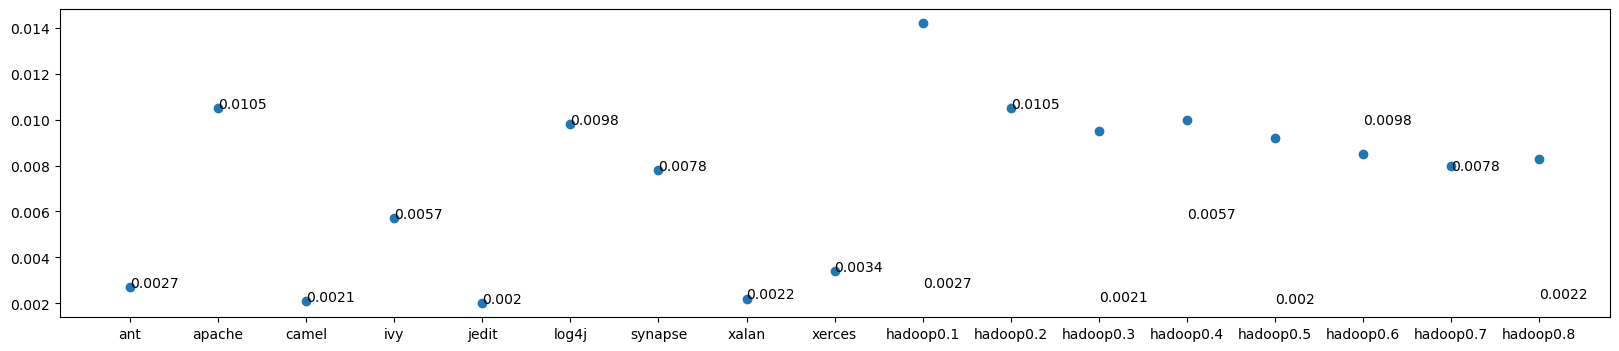
\includegraphics[width=0.99\textwidth]{figures/dimensionality-T3.png}
        \caption{Dimensionality T3}
        \label{fig:dimensionality-t3}
    \end{subfigure}
    \caption{Dimensionality Measures}
    \label{fig:dimensionality}
\end{figure}

%%%%%%%%%%
\begin{figure}[h!]
    \centering
    \begin{subfigure}{0.496\textwidth}
        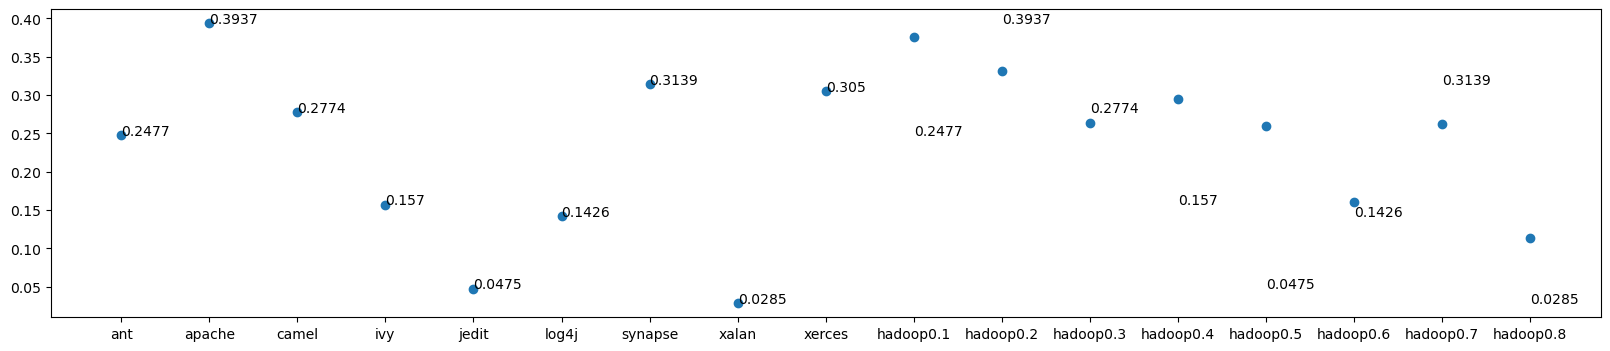
\includegraphics[width=0.99\textwidth]{figures/linearity-L1.png}
        \caption{Linearity L1}
        \label{fig:linearity-l1}
    \end{subfigure}
    \begin{subfigure}{0.496\textwidth}
        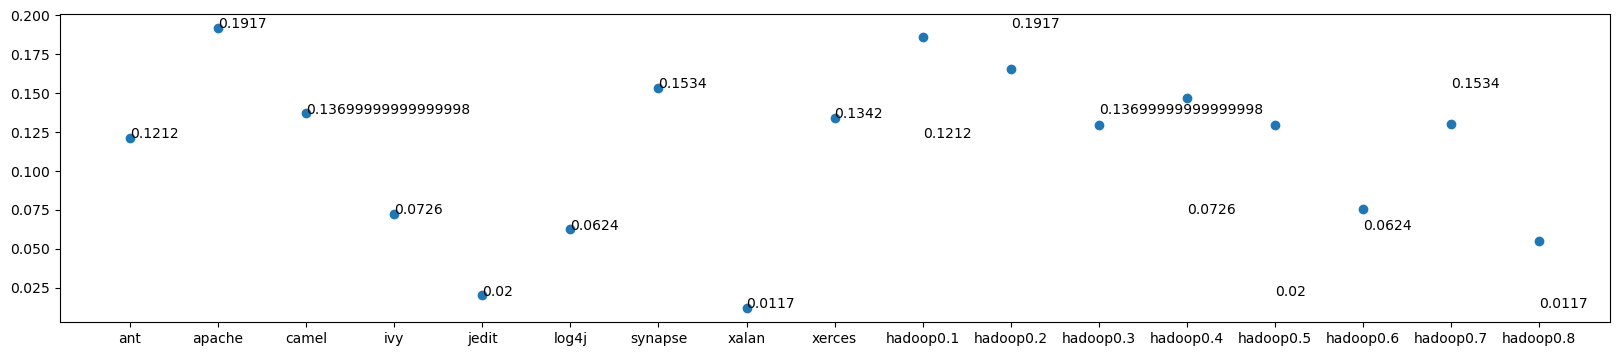
\includegraphics[width=0.99\textwidth]{figures/linearity-L2.png}
        \caption{Linearity L2}
        \label{fig:linearity-l2}
    \end{subfigure}
\end{figure}
\begin{figure}[h!]\ContinuedFloat
    \centering
    \begin{subfigure}{0.496\textwidth}
        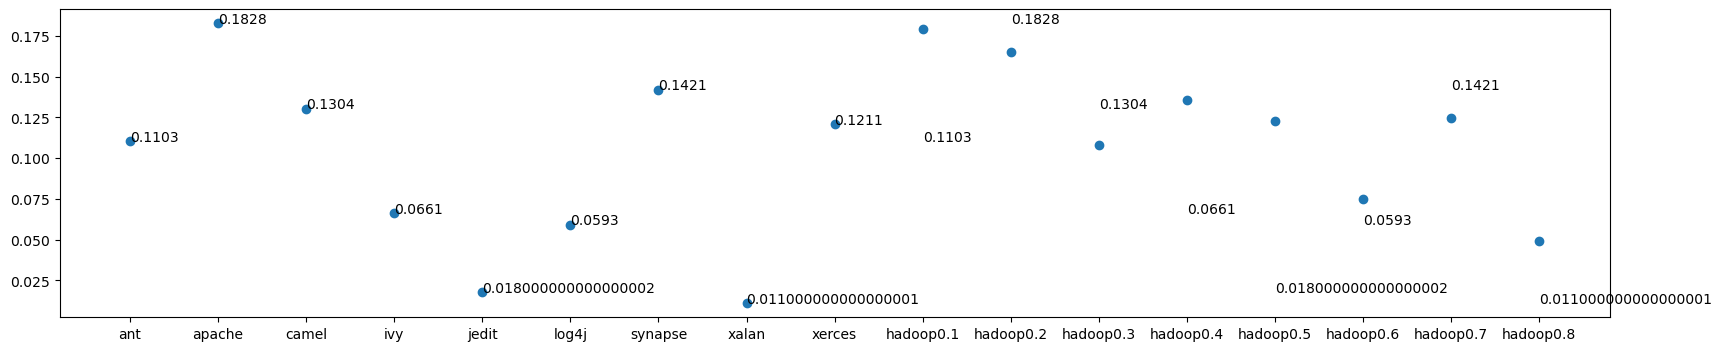
\includegraphics[width=0.99\textwidth]{figures/linearity-L3.png}
        \caption{Linearity L3}
        \label{fig:linearity-l3}
    \end{subfigure}
    \caption{Linearity Measures}
    \label{fig:linearity}
\end{figure}

%%%%%%%%%%
\begin{figure}[h!]
    \centering
    \begin{subfigure}{0.496\textwidth}
        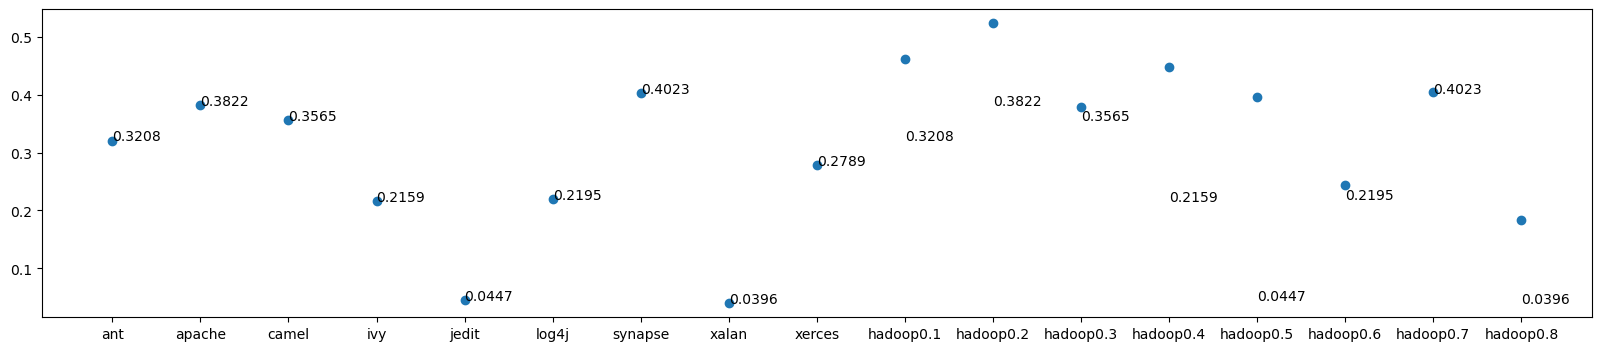
\includegraphics[width=0.99\textwidth]{figures/neighborhood-N1.png}
        \caption{Neighborhood N1}
        \label{fig:neighborhood-n1}
    \end{subfigure}
    \begin{subfigure}{0.496\textwidth}
        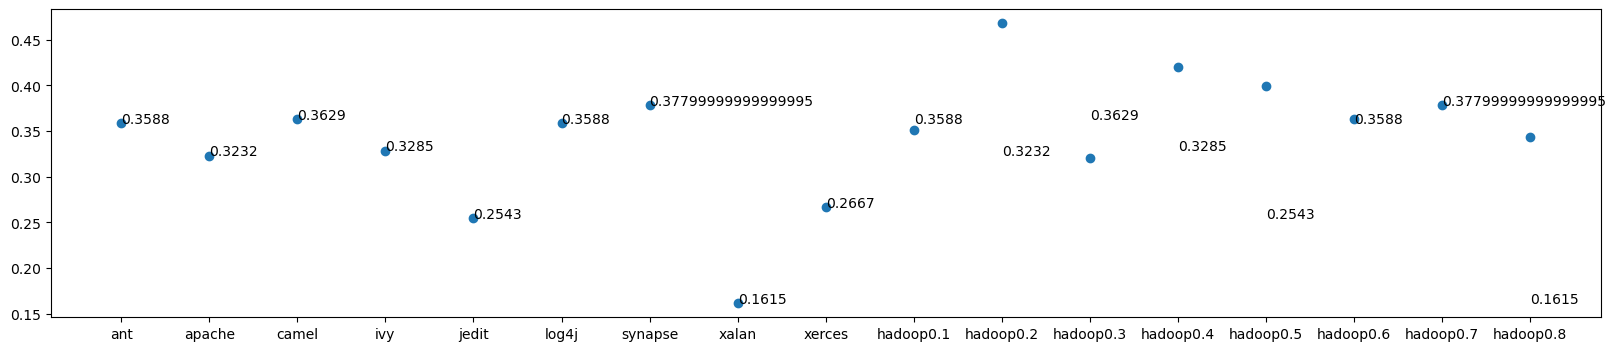
\includegraphics[width=0.99\textwidth]{figures/neighborhood-N2.png}
        \caption{Neighborhood N2}
        \label{fig:neighborhood-n2}
    \end{subfigure}
\end{figure}
\begin{figure}[h!]\ContinuedFloat
    \centering
    \begin{subfigure}{0.496\textwidth}
        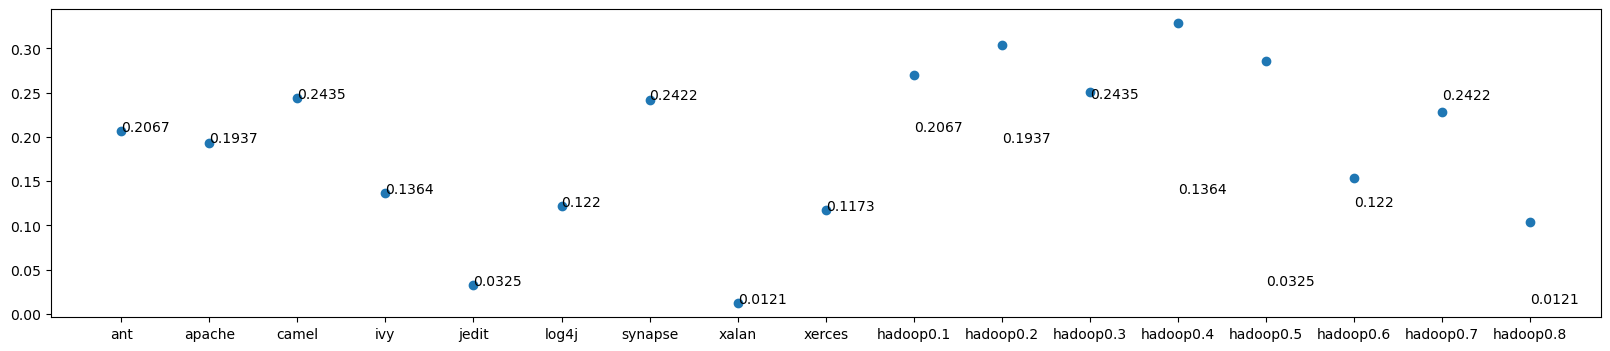
\includegraphics[width=0.99\textwidth]{figures/neighborhood-N3.png}
        \caption{Neighborhood N3}
        \label{fig:neighborhood-n3}
    \end{subfigure}
    \begin{subfigure}{0.496\textwidth}
        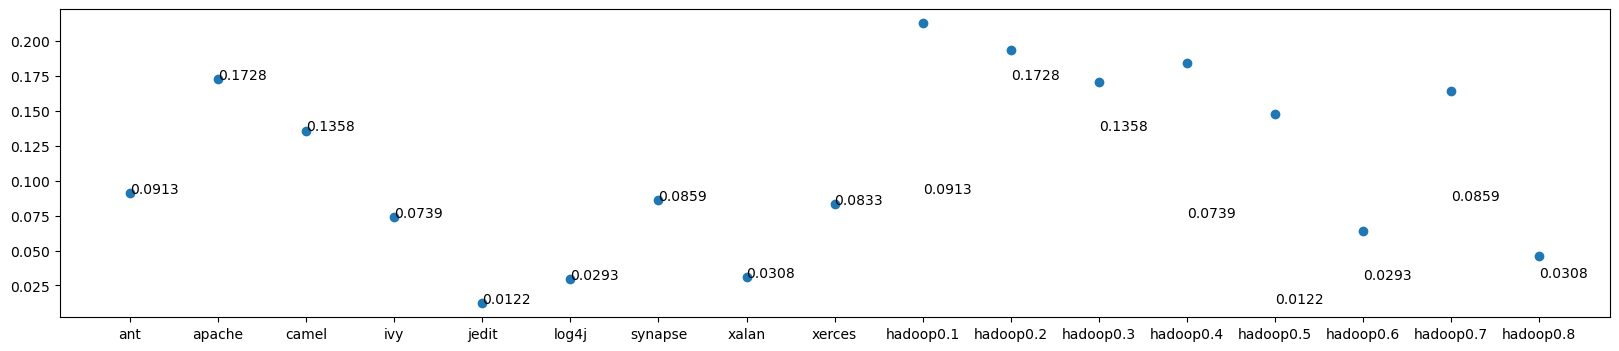
\includegraphics[width=0.99\textwidth]{figures/neighborhood-N4.png}
        \caption{Neighborhood N4}
        \label{fig:neighborhood-n4}
    \end{subfigure}
\end{figure}
\begin{figure}[h!]\ContinuedFloat
    \centering
    \begin{subfigure}{0.496\textwidth}
        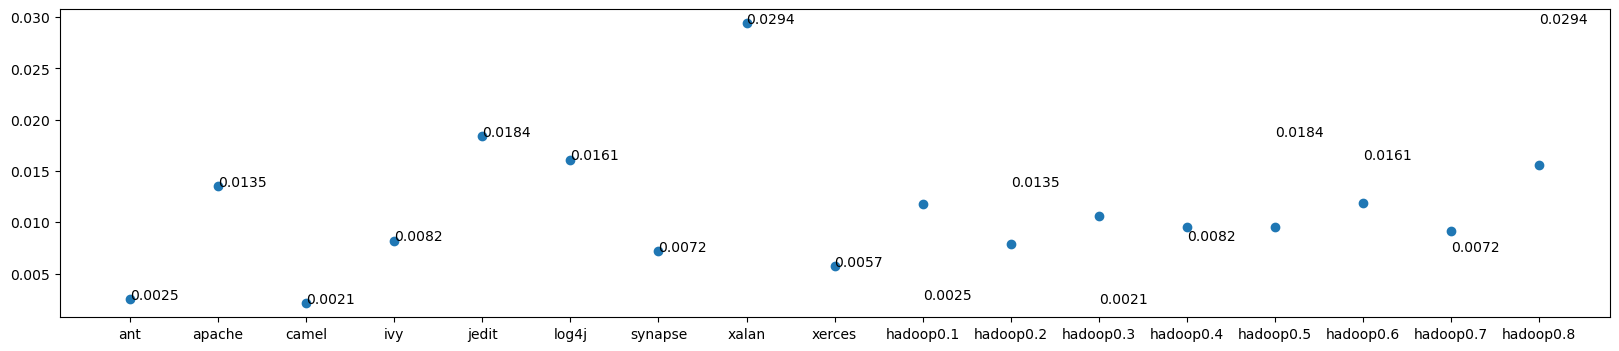
\includegraphics[width=0.99\textwidth]{figures/neighborhood-T1.png}
        \caption{Neighborhood T1}
        \label{fig:neighborhood-t1}
    \end{subfigure}
    \begin{subfigure}{0.496\textwidth}
        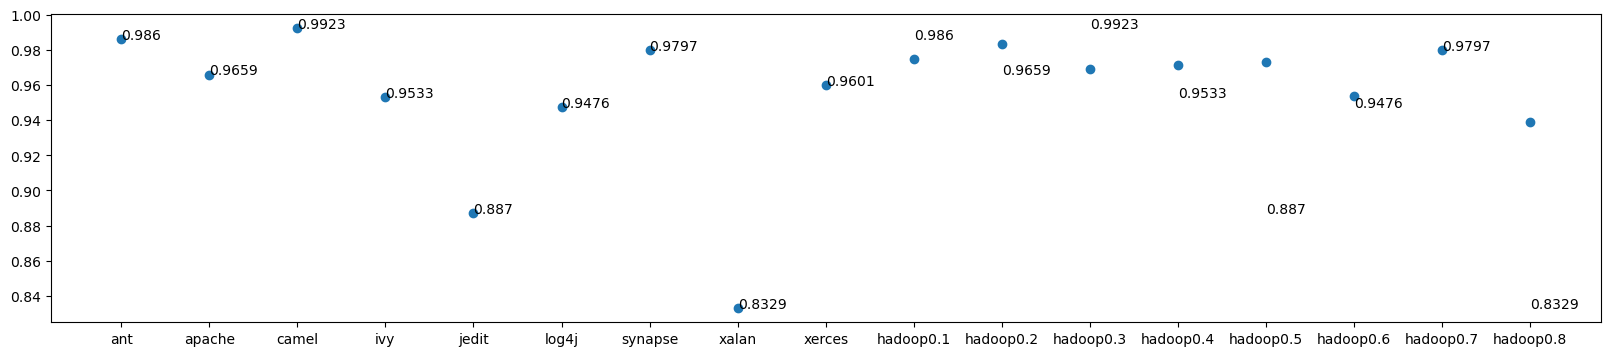
\includegraphics[width=0.99\textwidth]{figures/neighborhood-LSC.png}
        \caption{Neighborhood LSC}
        \label{fig:neighborhood-lsc}
    \end{subfigure}
    \caption{Neighborhood Measures}
    \label{fig:neighborhood}
\end{figure}

%%%%%%%%%%
\begin{figure}[h!]
    \centering
    \begin{subfigure}{0.496\textwidth}
        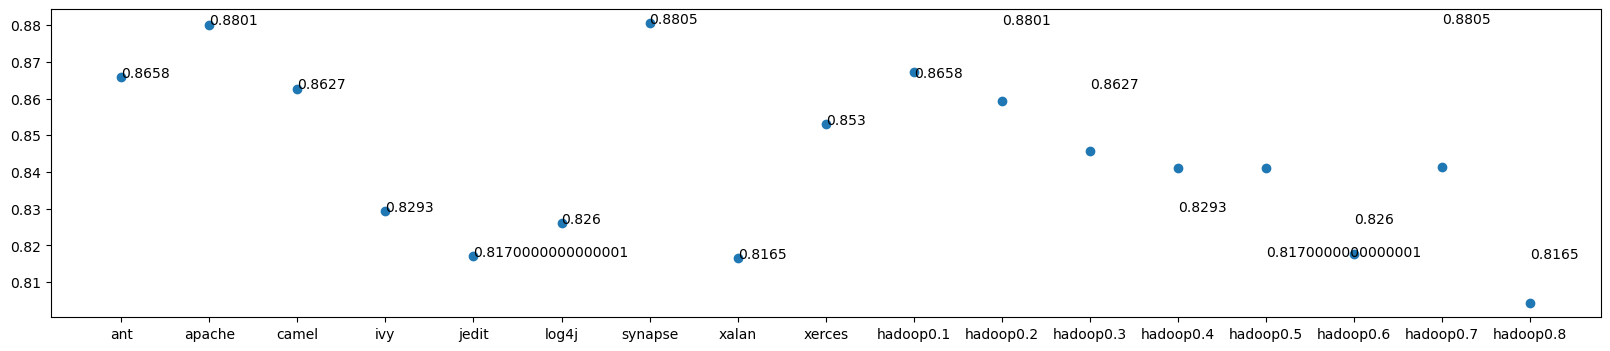
\includegraphics[width=0.99\textwidth]{figures/network-Density.png}
        \caption{Network Density}
        \label{fig:network-density}
    \end{subfigure}
    \begin{subfigure}{0.496\textwidth}
        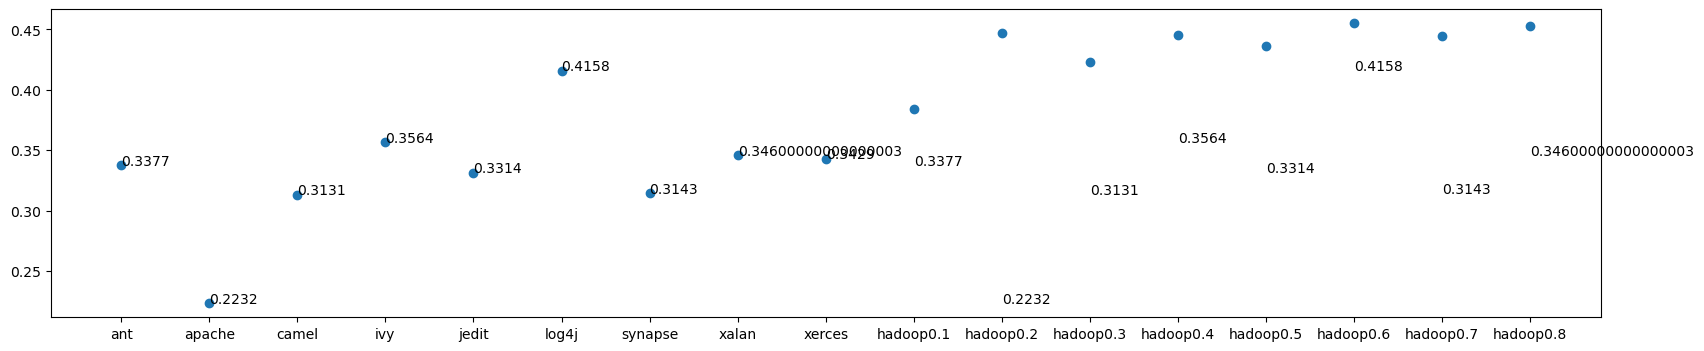
\includegraphics[width=0.99\textwidth]{figures/network-ClsCoef.png}
        \caption{Network ClsCoef}
        \label{fig:network-clscoef}
    \end{subfigure}
\end{figure}
\begin{figure}[h!]\ContinuedFloat
    \centering
    \begin{subfigure}{0.496\textwidth}
        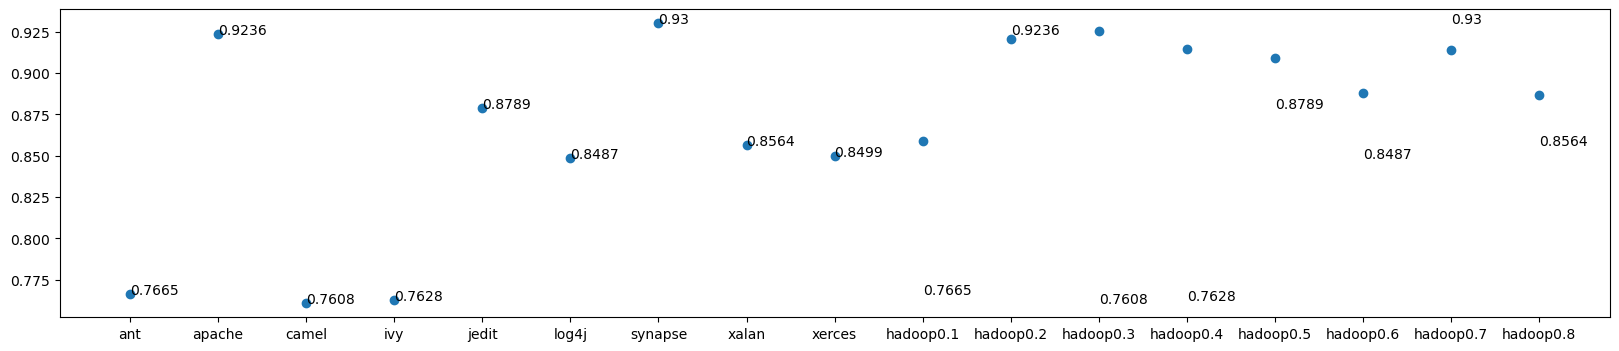
\includegraphics[width=0.99\textwidth]{figures/network-Hubs.png}
        \caption{Network Hubs}
        \label{fig:network-hubs}
    \end{subfigure}
    \caption{Network Measures}
    \label{fig:network}
\end{figure}

%%%%%%%%%%
\begin{figure}[h!]
    \centering
    \begin{subfigure}{0.496\textwidth}
        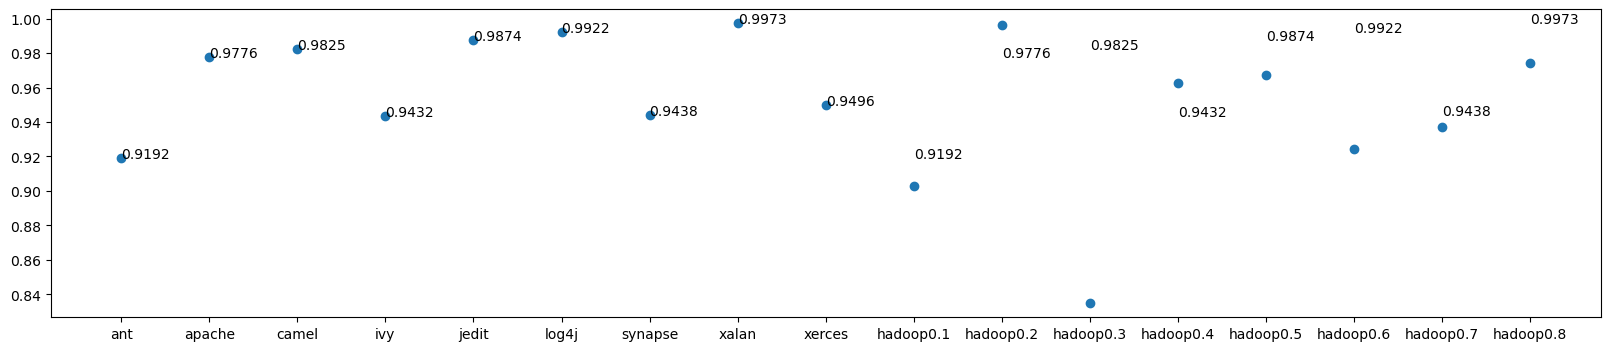
\includegraphics[width=0.99\textwidth]{figures/overlap-F1.png}
        \caption{Overlap F1}
        \label{fig:overlap-f1}
    \end{subfigure}
    \begin{subfigure}{0.496\textwidth}
        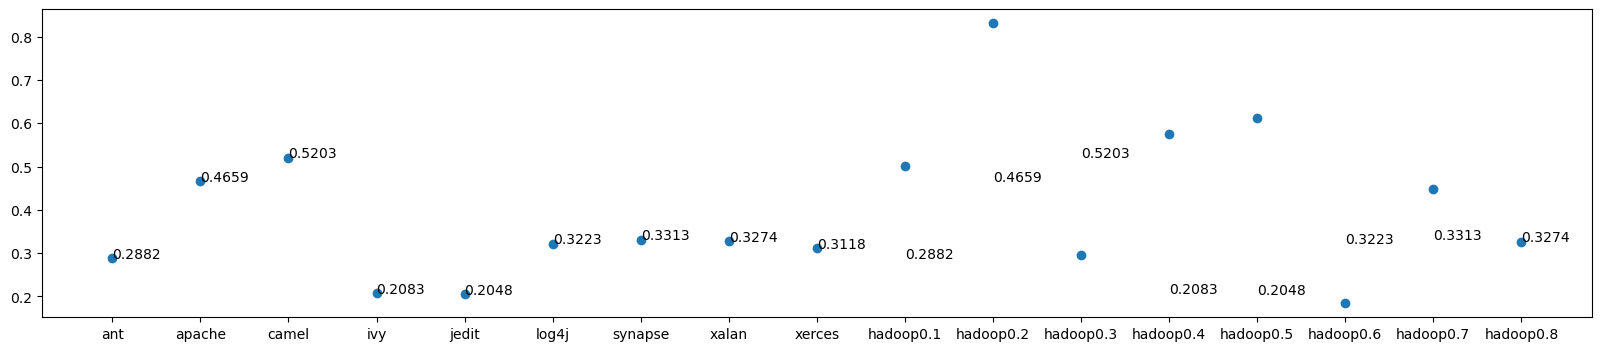
\includegraphics[width=0.99\textwidth]{figures/overlap-F1v.png}
        \caption{Overlap F1v}
        \label{fig:overlap-f1v}
    \end{subfigure}
\end{figure}
\begin{figure}[h!]\ContinuedFloat
    \centering
    \begin{subfigure}{0.496\textwidth}
        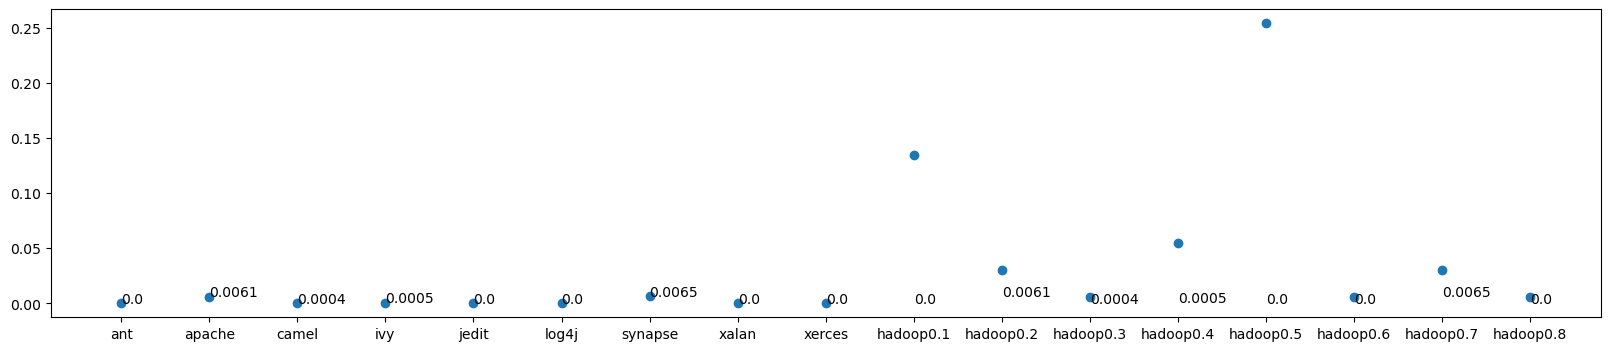
\includegraphics[width=0.99\textwidth]{figures/overlap-F2.png}
        \caption{Overlap F2}
        \label{fig:overlap-f2}
    \end{subfigure}
    \begin{subfigure}{0.496\textwidth}
        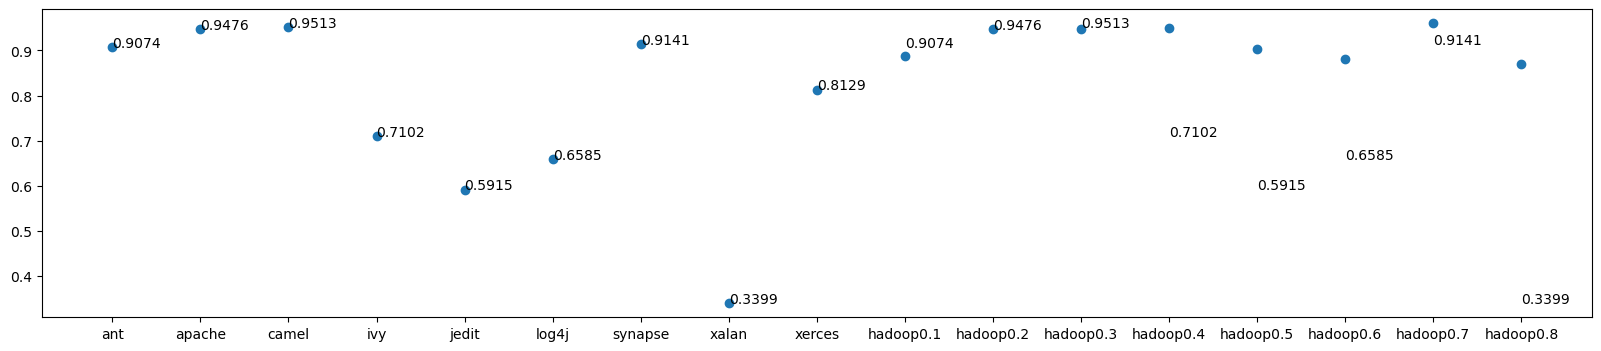
\includegraphics[width=0.99\textwidth]{figures/overlap-F3.png}
        \caption{Overlap F3}
        \label{fig:overlap-f3}
    \end{subfigure}
\end{figure}
\begin{figure}[h!]\ContinuedFloat
    \centering
    \begin{subfigure}{0.496\textwidth}
        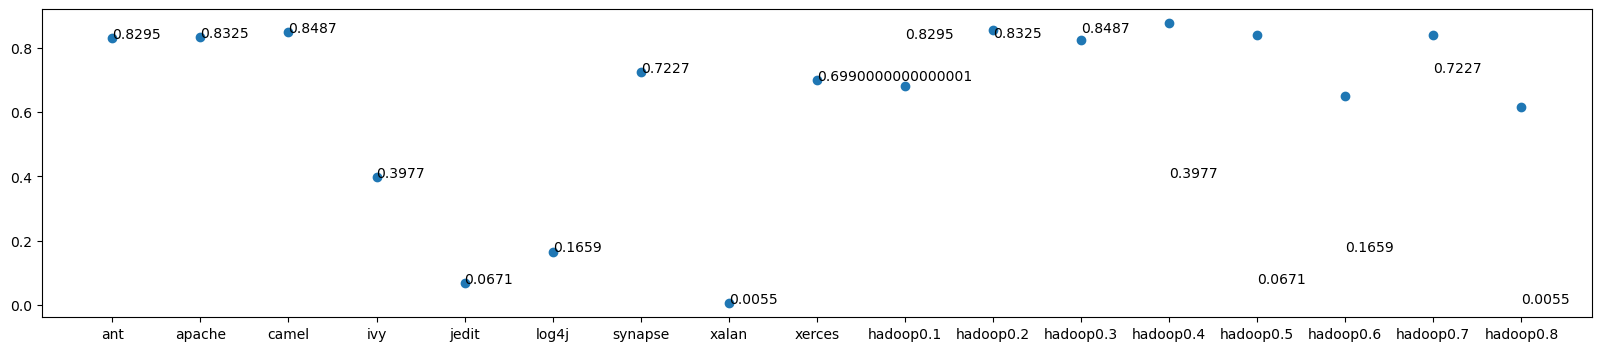
\includegraphics[width=0.99\textwidth]{figures/overlap-F4.png}
        \caption{Overlap F4}
        \label{fig:overlap-f4}
    \end{subfigure}
    \caption{Overlap Measures}
    \label{fig:overlap}
\end{figure}

%%%%%%%%%%
\begin{figure}[h!]
    \centering
    \begin{subfigure}{0.496\textwidth}
        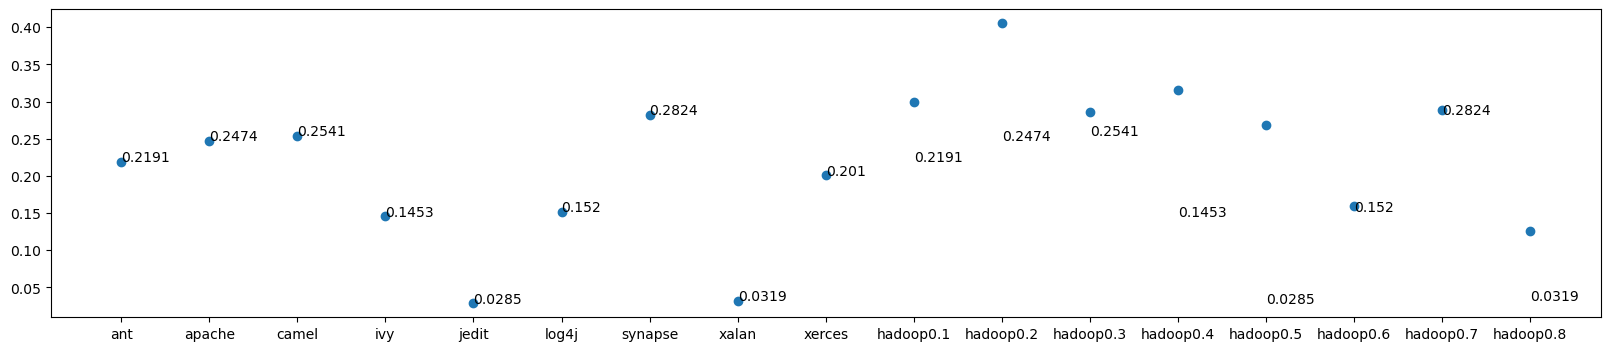
\includegraphics[width=0.99\textwidth]{figures/smoothness-S1.png}
        \caption{Smoothness S1}
        \label{fig:smoothness-s1}
    \end{subfigure}
    \begin{subfigure}{0.496\textwidth}
        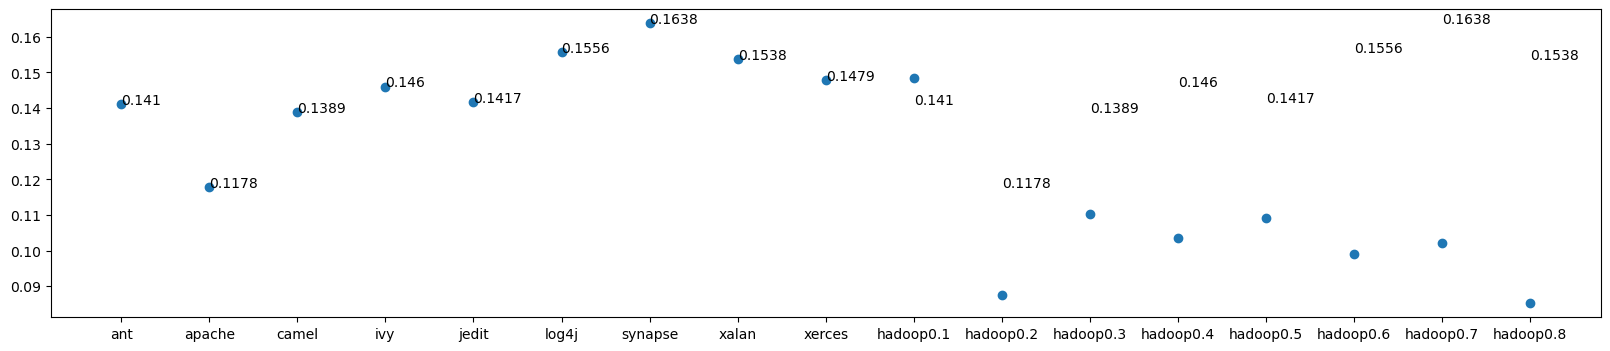
\includegraphics[width=0.99\textwidth]{figures/smoothness-S2.png}
        \caption{Smoothness S2}
        \label{fig:smoothness-s2}
    \end{subfigure}
\end{figure}
\begin{figure}[h!]\ContinuedFloat
    \centering
    \begin{subfigure}{0.496\textwidth}
        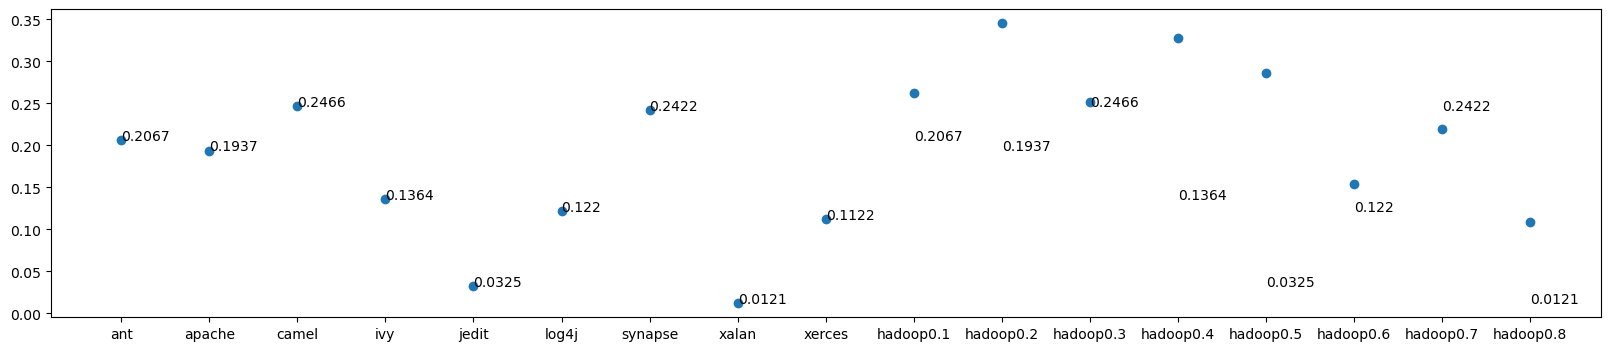
\includegraphics[width=0.99\textwidth]{figures/smoothness-S3.png}
        \caption{Smoothness S3}
        \label{fig:smoothness-s3}
    \end{subfigure}
    \begin{subfigure}{0.496\textwidth}
        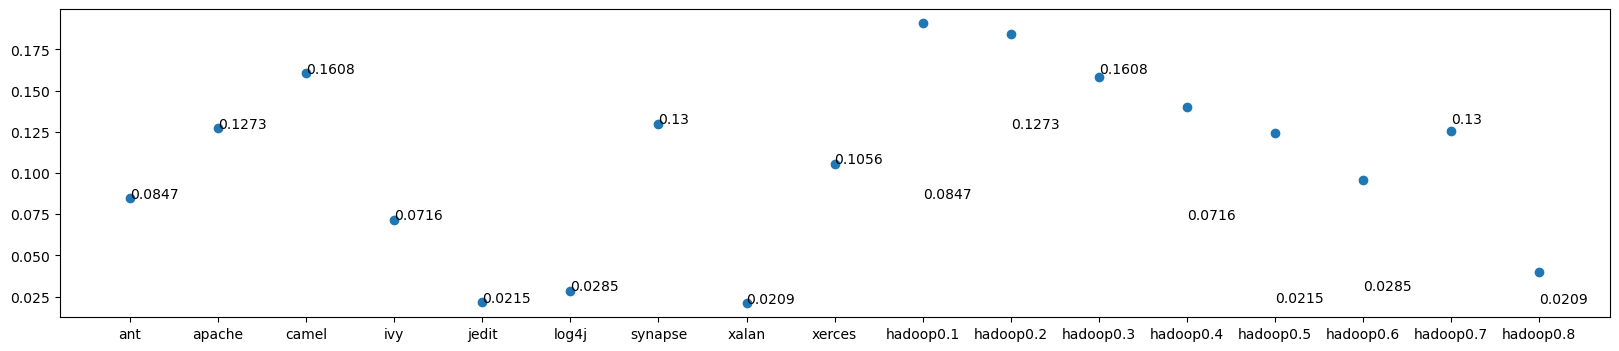
\includegraphics[width=0.99\textwidth]{figures/smoothness-S4.png}
        \caption{Smoothness S4}
        \label{fig:smoothness-s4}
    \end{subfigure}
    \caption{Smoothness Measures}
    \label{fig:smoothness}
\end{figure}

This way it is easier to compare results through datasets and metrics. To see 
the whole extent of the numerical values, see the tables at 
Appendix~\ref{chp:tables}. The data is summarized in tables \ref{sec:compl-oo} 
and \ref{sec:compl-hadoop}. To see the images in more detail (bigger) go to 
Appendix~\ref{chp:figures}, Section~\ref{sec:fig-compl-metrics}.

Further results are compared and discussed in Section~\ref{sec:compresults}.

%%%%%%%%%%%%%%%%%%%%%%%%%%%%%%%%%%%%%%%%%%%%%%%%%%%%%%%%%%%%%%%%%%%%%%
\subsection{Cross Validation Analysis}\label{sec:exp-kfold}

This experiment tries to find the impact of applying the $K$-fold 
Cross-Validation. It is a widely extended technique in data science that brings 
a solution to the problem of performing testing to a data set with no separate 
training data - the same instances in a given dataset should not be used for 
both training and testing a classifier at the same time, instead data can be 
divided so a portion is used for training and another separate portion for 
testing/validation. Cross validation allows us to estimate the performance of 
the model trained by the whole dataset dividing it into $k$ folds as follows:

\begin{itemize}
    \item Training set which is known data by the classifier, and used to train 
	it. It represents $k-1/k$ parts of the original set.
    \item Testing set, also known as validation set which corresponds to unseen 
	data for trained classifier used to test its performance. It usually is 
	$1/k$ of the original dataset.
\end{itemize}

Then, the average of carrying out $k$ iterations, same as the number of folds 
(parts/divisions) of the dataset, is calculated. On each iteration, the 
\textit{testing set} is rotated to another unused fold\footnote{The data in the 
different folds does not change throughout the cross validation process.} of the 
data - no testing set is repeated, which means that each fold is used only once 
for\textit{testing} purposes. 

The most common values for $k$ (folds) used in data science are 5 and 10. For 
this experiment, $k$ has been selected as $k=5$, as a common value of $k$ was 
needed for all experiments and some of the datasets did not have enough samples 
for a larger value of $k$.

The algorithm that analyses the performance of each fold and the calculates the 
mean performance can be simplified as the one explained in the 
Algorithm~\ref{alg:kfold}.

\begin{breakablealgorithm}
    \caption{Metrics Analysis on K-fold}
    \footnotesize
    \label{alg:kfold}
    \begin{algorithmic}[1]
        \Require $\mathcal{D}$ dataset
        \State inputs, targets $\leftarrow$ $\mathcal{D}$
    
        \State k $\leftarrow$ 5
        \State kf $\leftarrow$ kfold(k)
        \State splits $\leftarrow$ kf.split(inputs)
        
        \ForAll {$train_{i}$, $test_{i}$ in splits}
        	\State $x_{train}$, $x_{test}$ $\leftarrow$ inputs.get($train_{i}$), inputs.get($test_{i}$)
        	\State $y_{train}$, $y_{test}$ $\leftarrow$ targets.get($train_{i}$), targets.get($test_{i}$)
        	
        	\State clf $\leftarrow$ trainNetwork($x_{train}$, $y_{train}$)
        	
        	\State confusionMatrix($x_{test}$, $y_{test}$, clf)
        \EndFor
        \State calculateMeanPerformance(clf)
    \end{algorithmic}
\end{breakablealgorithm}

The Python script used for this experiment can be found in 
Appendix~\ref{chp:pythoncode}, Section~\ref{sec:exp-kfold-code}. It basically
separates a dataset into folds and calculates the performance metrics for each 
fold, to later on compute the mean value of those metrics for the entire dataset.

With the \textit{confusion matrix} other metrics are calculated such as 
$recall$, $MCC$, etc. Those metrics are then compared in Tables~\ref{tab:kfold} 
and~\ref{tab:kfold2}, for each specific dataset (to see the full extent of the 
comparison we refer to Section~\ref{sec:compresults}. For the sake of 
simplicity, only two tables of the aforementioned resulting datasets. 
Table~\ref{tab:kfold} shows the results obtained from Apache dataset.

\begin{center}
\begin{longtable}{ | r  l | c | c | c | c | c | c | c | }
\caption{Cross-Validation Results --- Apache Dataset}\label{tab:kfold} \\

\hline
\textbf{\emph{Fold}} & \textbf{\emph{Function}} & \emph{Precision} & \emph{Recall}  & \emph{Fall Out} & \emph{Balanced} & \emph{F1} & \emph{MCC} & \emph{AUC} \\
\hline
\endfirsthead
\hline
\multicolumn{9}{c}{\tablename\ \thetable\ -- \textit{Continued from previous page}} \\
\hline
\textbf{\emph{Fold}} & \textbf{\emph{Function}} & \emph{Precision} & \emph{Recall}  & \emph{Fall Out} & \emph{Balanced} & \emph{F1} & \emph{MCC} & \emph{AUC} \\
\hline
\endhead
\hline
\multicolumn{9}{r}{\textit{Continued on next page}}
\endfoot
\hline
\endlastfoot

\multirow{3}{*}{\textbf{1}} & \textbf{Naive Bayes} & 
0.4286 & 0.1579 & 0.200  & 0.4789 & 0.2308 & -0.0548 & 0.4789 \\
& \textbf{Decision Tree} & 
0.8235 & 0.7368 & 0.1500 & 0.7934 & 0.7778 &  0.5915 & 0.7934 \\
& \textbf{Nearest Centroid} &
0.3333 & 0.3158 & 0.6000 & 0.3579 & 0.3243 & -0.2850 & 0.3579 \\
\hline
\multirow{3}{*}{\textbf{2}} & \textbf{Naive Bayes} & 
0.5000 & 0.0800 & 0.1538 & 0.4631 & 0.1379 & -0.1142 & 0.4631 \\
& \textbf{Decision Tree} & 
0.8095 & 0.6800 & 0.3077 & 0.6862 & 0.7391 &  0.3552 & 0.6862 \\
& \textbf{Nearest Centroid} &
0.5000 & 0.1600 & 0.3077 & 0.4262 & 0.2424 & -0.1719 & 0.4262 \\
\hline
\multirow{3}{*}{\textbf{3}} & \textbf{Naive Bayes} & 
0.5000 & 0.0909 & 0.1250 & 0.4830 & 0.1538 & -0.0548 & 0.4830 \\
& \textbf{Decision Tree} & 
0.8462 & 0.5000 & 0.1250 & 0.6875 & 0.6286 &  0.3903 & 0.6875  \\
& \textbf{Nearest Centroid} &
0.4000 & 0.1818 & 0.3750 & 0.4034 & 0.2500 & -0.2166 & 0.4034 \\
\hline
\multirow{3}{*}{\textbf{4}} & \textbf{Naive Bayes} & 
0.3333 & 0.8182 & 0.6667 & 0.5758 & 0.4737 & 0.1515 & 0.5758 \\
& \textbf{Decision Tree} & 
0.5833 & 0.6364 & 0.1852 & 0.7256 & 0.6087 & 0.4402 & 0.7256 \\
& \textbf{Nearest Centroid} &
0.8000 & 0.7273 & 0.0741 & 0.8266 & 0.7619 & 0.6727 & 0.8266 \\
\hline
\multirow{3}{*}{\textbf{5}} & \textbf{Naive Bayes} & 
0.3043 & 1.0000 & 0.5161 & 0.7419 & 0.4667 & 0.3838 & 0.7419 \\
& \textbf{Decision Tree} & 
0.5000 & 1.0000 & 0.2258 & 0.8871 & 0.6667 & 0.6222 & 0.8871 \\
& \textbf{Nearest Centroid} &
0.4545 & 0.7143 & 0.1935 & 0.7604 & 0.5556 & 0.4451 & 0.7604 \\
\hline
\hline
% Mean
\multirow{3}{*}{\textbf{Mean}} & \textbf{Naive Bayes} & 
0.4132 & 0.4294 & 0.3323 & 0.5485 & 0.2926 & 0.0623 & 0.5485 \\
& \textbf{Decision Tree} & 
0.7125 & 0.7106 & 0.1987 & 0.7560 & 0.6842 & 0.4799 & 0.7560 \\
& \textbf{Nearest Centroid} &
0.4976 & 0.4198 & 0.3101 & 0.5549 & 0.4268 & 0.0889 & 0.5549 \\
\hline
\end{longtable}
\end{center}

The second example shown in Table~\ref{tab:kfold2} was obtained on the 
experiment performed over the Hadoop (v0.8) dataset.

\begin{center}
\begin{longtable}{ | r  l | c | c | c | c | c | c | c | }
\caption{Cross-Validation Results ---  Hadoop 0.8 Dataset}\label{tab:kfold2} \\

\hline
\textbf{\emph{Fold}} & \textbf{\emph{Function}} & \emph{Precision} & \emph{Recall}  & \emph{Fall Out} & \emph{Balanced} & \emph{F1} & \emph{MCC} & \emph{AUC} \\
\hline
\endfirsthead
\hline
\multicolumn{9}{c}{\tablename\ \thetable\ -- \textit{Continued from previous page}} \\
\hline
\textbf{\emph{Fold}} & \textbf{\emph{Function}} & \emph{Precision} & \emph{Recall}  & \emph{Fall Out} & \emph{Balanced} & \emph{F1} & \emph{MCC} & \emph{AUC} \\
\hline
\endhead
\hline
\multicolumn{9}{r}{\textit{Continued on next page}}
\endfoot
\hline
\endlastfoot

\multirow{3}{*}{\textbf{1}} & \textbf{Naive Bayes} & 
1.0000 & 0.1250 & 0.0000 & 0.5625 & 0.2222 & 0.3262  & 0.5625 \\
& \textbf{Decision Tree} & 
0.0000 & 0.0000 & 0.0250 & 0.4875 & 0.0000 & -0.0652 & 0.4875 \\
& \textbf{Nearest Centroid} &
0.1667 & 1.0000 & 1.0000 & 0.5000 & 0.2857 & 0.0000  & 0.5000 \\
\hline
\multirow{3}{*}{\textbf{2}} & \textbf{Naive Bayes} & 
0.0000 & 0.0000 & 0.1064 & 0.4468 & 0.0000 & -0.0497 & 0.4468 \\
& \textbf{Decision Tree} & 
0.0000 & 0.0000 & 0.1064 & 0.4468 & 0.0000 & -0.0497 & 0.4468 \\
& \textbf{Nearest Centroid} &
0.0208 & 1.0000 & 1.0000 & 0.5000 & 0.0408 & 0.0000 & 0.5000 \\
\hline
\multirow{3}{*}{\textbf{3}} & \textbf{Naive Bayes} & 
0.0000 & 0.0000 & 0.0851 & 0.4574 & 0.0000 & -0.0440 & 0.4574 \\
& \textbf{Decision Tree} & 
0.0000 & 0.0000 & 0.0851 & 0.4574 & 0.0000 & -0.0440 & 0.4574 \\
& \textbf{Nearest Centroid} &
0.0208 & 1.0000 & 1.0000 & 0.5000 & 0.0408 &  0.0000 & 0.5000 \\
\hline
\multirow{3}{*}{\textbf{4}} & \textbf{Naive Bayes} & 
0.3333 & 0.2500 & 0.0455 & 0.6023 & 0.2857 &  0.2335 & 0.6023 \\
& \textbf{Decision Tree} & 
0.0000 & 0.0000 & 0.0426 & 0.4787 & 0.0000 & -0.0304 & 0.4787 \\
& \textbf{Nearest Centroid} &
0.0000 & 0.0000 & 0.0227 & 0.4886 & 0.0000 & -0.0440 & 0.4886 \\
\hline
\multirow{3}{*}{\textbf{5}} & \textbf{Naive Bayes} & 
0.0000 & 0.0000 & 0.0000 & 0.5000 & 0.0000 & 0.0000 & 0.5000 \\
& \textbf{Decision Tree} & 
0.0000 & 0.0000 & 0.0000 & 0.5000 & 0.0000 & 0.0000 & 0.5000 \\
& \textbf{Nearest Centroid} &
0.0000 & 0.0000 & 0.0000 & 0.5000 & 0.0000 & 0.0000 & 0.5000 \\
\hline
\hline
% Mean
\multirow{3}{*}{\textbf{Mean}} & \textbf{Naive Bayes} & 
0.26667 & 0.0750 & 0.0474 & 0.5138 & 0.1016 & 0.0932 & 0.5138 \\
& \textbf{Decision Tree} & 
0.0000 & 0.0000 & 0.0484 & 0.4758 & 0.0000 & -0.0446 & 0.4758 \\
& \textbf{Nearest Centroid} &
0.0417 & 0.6000 & 0.6045 & 0.4977 & 0.0735 & -0.0088 & 0.4977 \\
\hline
\end{longtable}
\end{center}

The inner results of each fold are not evaluated when analyzing the results of 
the experiments, but that data could be used to understand how data metrics 
(including imbalance) affect classification. The objective evaluated in this 
paper is to see if the metrics obtained for each dataset have any relation with 
the performance of the classifiers. 

%%%%%%%%%%%%%%%%%%%%%%%%%%%%%%%%%%%%%%%%%%%%%%%%%%%%%%%%%%%%%%%%%%%%%%
\subsection{Imbalance Experimental Work}

After experimenting with cross-validation, we now focus on if filters applied 
to the dataset have any effect on the quality of the trained classifier. In this
case, it is carried out by applying imbalance filters to the folds in the 
datasets (see Section~\ref{sec:imbtechniques} for more information on imbalance 
filters). Here, the following techniques were used in the experiments:

\begin{description}
    \item [Undersampling] Removing samples from majority class.
    \item [Oversampling] Creating new samples in the minority class.
\end{description}

%%%%%%%%%%%%%%%%%%%%%%%%%%%%%%%%%%%%%%%%%%%%%%%%%%%%%%%%%%%%
\subsubsection{Undersampling with Cross Validation}
\label{sec:kfoldunder}

For this experiment, one undersampling algorithm is applied 
(\ref{nearmiss}) to see how folds are affected by removing majority class 
samples, and therefore, looking at how it impacts the classification algorithm. 

The undersampling technique is not done on the whole dataset in advance, only 
the training folds are the ones that the undersampling algorithm is applied. 

The $k$ value chosen for cross validation is $k=5$. A simplification
of the procedure followed by this experiment can be found in the 
Algorithm~\ref{alg:kfoldunder}.

\begin{breakablealgorithm}
    \caption{Undersampling with Cross-Validation}
    \label{alg:kfoldunder}
    \begin{algorithmic}[1]
        \Require $\mathcal{D}$ dataset
        \State inputs, targets $\leftarrow$ $\mathcal{D}$
    
        \State k $\leftarrow$ 5
        \State kf $\leftarrow$ kfold(k)
        \State splits $\leftarrow$ kf.split(inputs)
        
        \State samplingStrategy $\leftarrow$ {0:50, 1:50} \Comment{Binary class with a post undersampling distribution of 50-50}
        \State randomState $\leftarrow$ 42
        
        \ForAll {$train_{i}$, $test_{i}$ in splits}
        	\State $x_{train}$, $x_{test}$ $\leftarrow$ inputs.get($train_{i}$), inputs.get($test_{i}$)
        	\State $y_{train}$, $y_{test}$ $\leftarrow$ targets.get($train_{i}$), targets.get($test_{i}$)
        	
        	\State X, Y = makeImbalance(
        	\State \quad $x_{train}$, $y_{train}$,
        	\State \quad samplingStrategy,
        	\State \quad randomState
        	\State )
        	
        	\State clf $\leftarrow$ classifier(NearMiss(2), GaussianNB())
        	\State clf $\leftarrow$ trainNetwork(X, Y)
        	
        	\State confusionMatrix($x_{test}$, $y_{test}$, clf)
        \EndFor
        \State calculateMeanPerformance(clf)
    \end{algorithmic}
\end{breakablealgorithm}

Similarly to the previous experiment, the following classification algorithms 
were used to measure performance of the alterations done on the dataset, i.e., 
(1) Naive Bayes (Gaussian), (2) Decision Tree and (3) kNN Nearest Centroid.

The experiment creates the same tables obtained in 
experiment~\ref{sec:exp-kfold}, that is why sharing all the resulting tables of 
this experiment would be unnecessary - the results evaluated here can be found 
in Section~\ref{sec:compresults}. That is why only two of them have been 
included into this dissertation. The Apache dataset experiment (see 
Table~\ref{tab:kfoldunder}).

\begin{center}
\begin{longtable}{ | r  l | c | c | c | c | c | c | c | }
\caption{Cross-validation with Undersampling Results --- Apache dataset}
\label{tab:kfoldunder} 
\\
\hline
\textbf{\emph{Fold}} & \textbf{\emph{Function}} & 
\emph{Precision} & \emph{Recall}  & \emph{Fall Out} & 
\emph{Balanced} & \emph{F1} & \emph{MCC} & \emph{AUC} \\
\hline
\endfirsthead
\hline
\multicolumn{9}{c}{\tablename\ \thetable\ -- \textit{Continued from previous page}} \\
\hline
\textbf{\emph{Fold}} & \textbf{\emph{Function}} & 
\emph{Precision} & \emph{Recall}  & \emph{Fall Out} & 
\emph{Balanced} & \emph{F1} & \emph{MCC} & \emph{AUC} \\
\hline
\endhead
\hline
\multicolumn{9}{r}{\textit{Continued on next page}}
\endfoot
\hline
\endlastfoot
\hline

\multirow{3}{*}{\textbf{1}} & \textbf{Naive Bayes} & 
0.5556 & 0.8824 & 0.5455 & 0.6684 & 0.6818 &  0.3620 & 0.6684 \\
& \textbf{Decision Tree} & 
0.7000 & 0.8235 & 0.2727 & 0.7754 & 0.7568 &  0.5464 & 0.7754 \\
& \textbf{Nearest Centroid} &
0.4167 & 0.2941 & 0.3182 & 0.4880 & 0.3448 & -0.0259 & 0.4880 \\
\hline
\multirow{3}{*}{\textbf{2}} & \textbf{Naive Bayes} & 
0.5500 & 0.7333 & 0.3913 & 0.6710 & 0.6286 &  0.3348 & 0.6710 \\
& \textbf{Decision Tree} & 
0.5500 & 0.7333 & 0.3913 & 0.6710 & 0.6286 &  0.3348 & 0.6710 \\
& \textbf{Nearest Centroid} &
0.3571 & 0.3333 & 0.3913 & 0.4710 & 0.3448 & -0.0587 & 0.4710  \\
\hline
\multirow{3}{*}{\textbf{3}} & \textbf{Naive Bayes} & 
0.7586 & 0.8800 & 0.5385 & 0.6708 & 0.8148 & 0.3811 & 0.6708 \\
& \textbf{Decision Tree} & 
0.8421 & 0.6400 & 0.2308 & 0.7046 & 0.7273 & 0.3883 & 0.7046 \\
& \textbf{Nearest Centroid} &
0.7000 & 0.2800 & 0.2308 & 0.5246 & 0.4000 & 0.0530 & 0.5246 \\
\hline
\multirow{3}{*}{\textbf{4}} & \textbf{Naive Bayes} & 
0.6667 & 0.7273 & 0.1481 & 0.7896 & 0.6957 & 0.5650 & 0.7896 \\
& \textbf{Decision Tree} & 
0.6667 & 0.7273 & 0.1481 & 0.7896 & 0.6957 & 0.5650 & 0.7896 \\
& \textbf{Nearest Centroid} &
0.3077 & 0.3636 & 0.3333 & 0.5152 & 0.3333 & 0.0290 & 0.5152 \\
\hline
\multirow{3}{*}{\textbf{5}} & \textbf{Naive Bayes} & 
0.5000 & 0.5625 & 0.4091 & 0.5767 & 0.5294 & 0.1517 & 0.5767 \\
& \textbf{Decision Tree} & 
0.6316 & 0.7500 & 0.3182 & 0.7159 & 0.6857 & 0.4264 & 0.7159 \\
& \textbf{Nearest Centroid} &
0.5556 & 0.3125 & 0.1818 & 0.5653 & 0.4000 & 0.1518 & 0.5653 \\
\hline
\multirow{3}{*}{\textbf{Mean}} & \textbf{Naive Bayes} & 
0.5928 & 0.6662 & 0.3917 & 0.6372 & 0.6059 & 0.2992 & 0.6372 \\
& \textbf{Decision Tree} & 
0.6781 & 0.7348 & 0.2722 & 0.7313 & 0.6988 & 0.4522 & 0.7313 \\
& \textbf{Nearest Centroid} &
0.4674 & 0.3167 & 0.2911 & 0.5128 & 0.3646 & 0.0298 & 0.5128 \\
\hline
\end{longtable}
\end{center}

And the result obtained on the same experiment for the Hadoop (v0.8)
experiment (see Table~\ref{tab:kfoldunder2}).

\begin{center}
\begin{longtable}{ | r  l | c | c | c | c | c | c | c | }
\caption{Cross-validation with Undersampling Results --- Hadoop 0.8}\label{tab:kfoldunder2} \\
\hline
\textbf{\emph{Fold}} & \textbf{\emph{Function}} & 
\emph{Precision} & \emph{Recall}  & \emph{Fall Out} & 
\emph{Balanced} & \emph{F1} & \emph{MCC} & \emph{AUC} \\
\hline
\endfirsthead
\hline
\multicolumn{9}{c}{\tablename\ \thetable\ -- \textit{Continued from previous page}} \\
\hline
\textbf{\emph{Fold}} & \textbf{\emph{Function}} & 
\emph{Precision} & \emph{Recall}  & \emph{Fall Out} & 
\emph{Balanced} & \emph{F1} & \emph{MCC} & \emph{AUC} \\
\hline
\endhead
\hline
\multicolumn{9}{r}{\textit{Continued on next page}}
\endfoot
\hline
\endlastfoot
\hline

\multirow{3}{*}{\textbf{1}} & \textbf{Naive Bayes} & 
0.1429 & 0.5000 & 0.1304 & 0.6848 & 0.2222 &  0.2092 & 0.6848 \\
& \textbf{Decision Tree} & 
0.1053 & 1.0000 & 0.3696 & 0.8152 & 0.1905 &  0.2576 & 0.8152 \\
& \textbf{Nearest Centroid} &
0.0345 & 0.5000 & 0.6087 & 0.4457 & 0.0645 & -0.0444 & 0.4457 \\
\hline
\multirow{3}{*}{\textbf{2}} & \textbf{Naive Bayes} & 
0.0000 & 0.0000 & 0.2667 & 0.3667 & 0.0000 & -0.1491 & 0.3667 \\
& \textbf{Decision Tree} & 
0.0833 & 0.3333 & 0.2444 & 0.5444 & 0.1333 &  0.0497 & 0.5444 \\
& \textbf{Nearest Centroid} &
0.0952 & 0.6667 & 0.4222 & 0.6222 & 0.1667 &  0.1193 & 0.6222 \\
\hline
\multirow{3}{*}{\textbf{3}} & \textbf{Naive Bayes} & 
0.0833 & 0.5000 & 0.2391 & 0.6304 & 0.1429 &  0.1204 & 0.6304\\
& \textbf{Decision Tree} & 
0.0000 & 0.0000 & 0.3261 & 0.3370 & 0.0000 & -0.1406 & 0.3370 \\
& \textbf{Nearest Centroid} &
0.0000 & 0.0000 & 0.4348 & 0.2826 & 0.0000 & -0.1762 & 0.2826 \\
\hline
\multirow{3}{*}{\textbf{4}} & \textbf{Naive Bayes} & 
0.1333 & 0.3333 & 0.3095 & 0.5119 & 0.1905 &  0.0170 & 0.5119 \\
& \textbf{Decision Tree} & 
0.1765 & 0.5000 & 0.3333 & 0.5833 & 0.2609 &  0.1153 & 0.5833 \\
& \textbf{Nearest Centroid} &
0.0625 & 0.1667 & 0.3571 & 0.4048 & 0.0909 & -0.1336 & 0.4048 \\
\hline
\multirow{3}{*}{\textbf{5}} & \textbf{Naive Bayes} & 
0.0000 & 0.0000 & 0.1556 & 0.4222 & 0.0000 & -0.1067 & 0.4222 \\
& \textbf{Decision Tree} & 
0.2000 & 0.6667 & 0.1778 & 0.7444 & 0.3077 &  0.2914 & 0.7444 \\
& \textbf{Nearest Centroid} &
0.0000 & 0.0000 & 0.2444 & 0.3778 & 0.0000 & -0.1408 & 0.3778 \\
\hline
\multirow{3}{*}{\textbf{Mean}} & \textbf{Naive Bayes} & 
0.0719 & 0.2667 & 0.2203 & 0.5232 & 0.1111 &  0.0182 & 0.5232 \\
& \textbf{Decision Tree} & 
0.1130 & 0.5000 & 0.2902 & 0.6049 & 0.1785 &  0.1147 & 0.6049 \\
& \textbf{Nearest Centroid} &
0.0384 & 0.2667 & 0.4134 & 0.4266 & 0.0644 & -0.0751 & 0.4266 \\
\hline
\end{longtable}
\end{center}

As it has been mentioned in Section~\ref{nearmiss}, there are several versions 
of \textit{Near Miss} algorithm. For this experiment it was used \textit{version 
2}. This undersampling algorithm selects the majority class samples with the 
least average distance to the 3 farthest minority class samples.

The analysis of the metrics obtained are discussed in 
Section~\ref{sec:compresults}.

%%%%%%%%%%%%%%%%%%%%%%%%%%%%%%%%%%%%%%%%%%%%%%%%%%%%%%%%%%%%
\subsubsection{Oversampling with Cross Validation}

In this experiment, similarly to Section~\ref{sec:kfoldunder}, an imbalance 
filter is used. In this case, the oversampling technique is implemented and is 
later on compared to other experiment results (see 
Section~\ref{sec:compresults}).

The technique has been applied to the different folds of the dataset, not to the
entire data. Once again, the dataset is divided into $k=5$ folds. 

The logic of the Python code experiment is summarized in 
Algorithm~\ref{alg:kfoldover}. The difference with the undersampling 
Algorithm~\ref{alg:kfoldunder} is that uses the SMOTE technique (see 
Section~\ref{smote}) instead of \textit{Near Miss} undersampling technique.

\begin{breakablealgorithm}
    \caption{Oversampling and K-fold on classification performance}
    \footnotesize
    \label{alg:kfoldover}
    \begin{algorithmic}[1]
        \Require $\mathcal{D}$ dataset
        \State inputs, targets $\leftarrow$ $\mathcal{D}$
    
        \State k $\leftarrow$ 5
        \State kf $\leftarrow$ kfold(k)
        \State splits $\leftarrow$ kf.split(inputs)
        
        \ForAll {$train_{i}$, $test_{i}$ in splits}
        	\State $x_{train}$, $x_{test}$ $\leftarrow$ inputs.get($train_{i}$), inputs.get($test_{i}$)
        	\State $y_{train}$, $y_{test}$ $\leftarrow$ targets.get($train_{i}$), targets.get($test_{i}$)
        	
        	\State clf $\leftarrow$ classifier(SMOTE(), GaussianNB())
        	\State clf $\leftarrow$ trainNetwork($x_{train}$, $y_{train}$)
        	
        	\State confusionMatrix($x_{test}$, $y_{test}$, clf)
        \EndFor
        \State calculateMeanPerformance(clf)
    \end{algorithmic}
\end{breakablealgorithm}

The classifiers used for this experiment are - (1) Naive Bayes (Gaussian); 
(2) Decision Tree; and (3) kNN Nearest Centroid.

Next we show two of the results obtained, fhe first one is the result on the 
Apache dataset (see Table~\ref{tab:kfoldover-apache}).

\begin{center}
\begin{longtable}{ | r  l | c | c | c | c | c | c | c | }
\caption{Oversampling with Cross Validation Results --- Apache dataset}
\label{tab:kfoldover-apache} 
\\

\hline
\textbf{\emph{Fold}} & \textbf{\emph{Function}} & 
\emph{Precision} & \emph{Recall}  & \emph{Fall Out} & 
\emph{Balanced} & \emph{F1} & \emph{MCC} & \emph{AUC} \\
\hline
\endfirsthead
\hline
\multicolumn{9}{c}{\tablename\ \thetable\ -- \textit{Continued from previous page}} \\
\hline
\textbf{\emph{Fold}} & \textbf{\emph{Function}} & 
\emph{Precision} & \emph{Recall}  & \emph{Fall Out} & 
\emph{Balanced} & \emph{F1} & \emph{MCC} & \emph{AUC} \\
\hline
\endhead
\hline
\multicolumn{9}{r}{\textit{Continued on next page}}
\endfoot
\hline
\endlastfoot

\multirow{3}{*}{\textbf{1}} & \textbf{Naive Bayes} & 
0.4286 & 0.1579 & 0.2000 & 0.4789 & 0.2308 & -0.0548 & 0.4789 \\
& \textbf{Decision Tree} & 
0.7222 & 0.6842 & 0.2500 & 0.7171 & 0.7027 &  0.4354 & 0.7171 \\
& \textbf{Nearest Centroid} &
0.3333 & 0.3158 & 0.6000 & 0.3579 & 0.3243 & -0.2850 & 0.3579 \\
\hline
\multirow{3}{*}{\textbf{2}} & \textbf{Naive Bayes} & 
0.5000 & 0.0800 & 0.1538 & 0.4631 & 0.1379 & -0.1142 & 0.4631 \\
& \textbf{Decision Tree} & 
0.8889 & 0.6400 & 0.1538 & 0.7431 & 0.7442 &  0.4619 & 0.7431 \\
& \textbf{Nearest Centroid} &
0.5000 & 0.1600 & 0.3077 & 0.4262 & 0.2424 & -0.1719 & 0.4262 \\
\hline
\multirow{3}{*}{\textbf{3}} & \textbf{Naive Bayes} & 
0.5000 & 0.0909 & 0.1250 & 0.4830 & 0.1538 & -0.0548 & 0.4830 \\
& \textbf{Decision Tree} & 
0.8000 & 0.5455 & 0.1875 & 0.6790 & 0.6486 &  0.3616 & 0.6790 \\
& \textbf{Nearest Centroid} &
0.4286 & 0.1364 & 0.2500 & 0.4432 & 0.2069 & -0.1447 & 0.4432 \\
\hline
\multirow{3}{*}{\textbf{4}} & \textbf{Naive Bayes} & 
0.3333 & 0.8182 & 0.6667 & 0.5758 & 0.4737 &  0.1515 & 0.5758 \\
& \textbf{Decision Tree} & 
0.5385 & 0.6364 & 0.2222 & 0.7071 & 0.5833 &  0.3959 & 0.7071 \\
& \textbf{Nearest Centroid} &
0.6000 & 0.5455 & 0.1481 & 0.6987 & 0.5714 &  0.4092 & 0.6987 \\
\hline
\multirow{3}{*}{\textbf{5}} & \textbf{Naive Bayes} & 
0.3182 & 1.0000 & 0.4839 & 0.7581 & 0.4828 & 0.4052 & 0.7581 \\
& \textbf{Decision Tree} & 
0.5000 & 1.0000 & 0.2258 & 0.8871 & 0.6667 & 0.6222 & 0.8871 \\
& \textbf{Nearest Centroid} &
0.4545 & 0.7143 & 0.1935 & 0.7604 & 0.5556 & 0.4451 & 0.7604 \\
\hline
\hline
% Mean
\multirow{3}{*}{\textbf{Mean}} & \textbf{Naive Bayes} & 
0.4160 & 0.4294 & 0.3259 & 0.5518 & 0.2958 & 0.0666 & 0.5518 \\
& \textbf{Decision Tree} & 
0.6899 & 0.7012 & 0.2079 & 0.7467 & 0.6691 & 0.4554 & 0.7467 \\
& \textbf{Nearest Centroid} &
0.4633 & 0.3744 & 0.2999 & 0.5373 & 0.3801 & 0.0505 & 0.5373 \\
\hline

\end{longtable}
\end{center}

The second example is the one from the Hadoop (v0.8) experiment (see 
Table~\ref{tab:kfoldover-hadoop}).

\begin{center}
\begin{longtable}{ | r  l | c | c | c | c | c | c | c | }
\caption{Oversampling with Cross-Validation Results --- Hadoop 0.8 dataset}\label{tab:kfoldover-hadoop} \\

\hline
\textbf{\emph{Fold}} & \textbf{\emph{Function}} & \emph{Precision} & \emph{Recall}  & \emph{Fall Out} & \emph{Balanced} & \emph{F1} & \emph{MCC} & \emph{AUC} \\
\hline
\endfirsthead
\hline
\multicolumn{9}{c}{\tablename\ \thetable\ -- \textit{Continued from previous page}} \\
\hline
\textbf{\emph{Fold}} & \textbf{\emph{Function}} & \emph{Precision} & \emph{Recall}  & \emph{Fall Out} & \emph{Balanced} & \emph{F1} & \emph{MCC} & \emph{AUC} \\
\hline
\endhead
\hline
\multicolumn{9}{r}{\textit{Continued on next page}}
\endfoot
\hline
\endlastfoot

\multirow{3}{*}{\textbf{1}} & \textbf{Naive Bayes} & 
0.1176 & 0.2500 & 0.3750 & 0.4375 & 0.1600 & -0.0974 & 0.4375 \\
& \textbf{Decision Tree} & 
0.2500 & 0.1250 & 0.0750 & 0.5250 & 0.1667 &  0.0674 & 0.5250 \\
& \textbf{Nearest Centroid} &
0.1667 & 1.0000 & 1.0000 & 0.5000 & 0.2857 &  0.0000 & 0.5000 \\
\hline
\multirow{3}{*}{\textbf{2}} & \textbf{Naive Bayes} & 
0.1000 & 1.0000 & 0.1915 & 0.9043 & 0.1818 &  0.2843 & 0.9043 \\
& \textbf{Decision Tree} & 
0.0000 & 0.0000 & 0.4468 & 0.2766 & 0.0000 & -0.1286 & 0.2766 \\
& \textbf{Nearest Centroid} &
0.0208 & 1.0000 & 1.0000 & 0.5000 & 0.0408 &  0.0000 & 0.5000 \\
\hline
\multirow{3}{*}{\textbf{3}} & \textbf{Naive Bayes} & 
0.0000 & 0.0000 & 0.1915 & 0.4043 & 0.0000 & -0.0701 & 0.4043 \\
& \textbf{Decision Tree} & 
0.0000 & 0.0000 & 0.1064 & 0.4468 & 0.0000 & -0.0497 & 0.4468 \\
& \textbf{Nearest Centroid} &
0.0208 & 1.0000 & 1.0000 & 0.5000 & 0.0408 &  0.0000 & 0.5000 \\
\hline
\multirow{3}{*}{\textbf{4}} & \textbf{Naive Bayes} & 
0.0667 & 0.5000 & 0.6364 & 0.4318 & 0.1176 & -0.0778 & 0.4318 \\
& \textbf{Decision Tree} & 
0.2500 & 0.2500 & 0.0682 & 0.5909 & 0.2500 &  0.1818 & 0.5909 \\
& \textbf{Nearest Centroid} &
0.0000 & 0.0000 & 0.0000 & 0.5000 & 0.0000 &  0.0000 & 0.5000 \\
\hline
\multirow{3}{*}{\textbf{5}} & \textbf{Naive Bayes} & 
0.0000 & 0.0000 & 0.0000 & 0.5000 & 0.0000 &  0.0000 & 0.5000 \\
& \textbf{Decision Tree} & 
0.0000 & 0.0000 & 0.0435 & 0.4783 & 0.0000 & -0.0435 & 0.4783 \\
& \textbf{Nearest Centroid} &
0.0000 & 0.0000 & 0.0000 & 0.5000 & 0.0000 &  0.0000 & 0.5000 \\
\hline
\hline
\multirow{3}{*}{\textbf{Mean}} & \textbf{Naive Bayes} & 
0.0569 & 0.3500 & 0.2789 & 0.5356 & 0.0919 &  0.0078 & 0.5356 \\
& \textbf{Decision Tree} & 
0.1000 & 0.0750 & 0.1480 & 0.4635 & 0.0833 &  0.0055 & 0.4635 \\
& \textbf{Nearest Centroid} &
0.0417 & 0.6000 & 0.6000 & 0.5000 & 0.0735 &  0.0000 & 0.5000 \\
\hline
\end{longtable}
\end{center}

The analysis of the metrics obtained are in Section~\ref{sec:compresults}.

%%%%%%%%%%%%%%%%%%%%%%%%%%%%%%%%%%%%%%%%%%%%%%%%%%%%%%%%%%%%%%%%%%%%%%
\subsection{Comparison of the Results and Discussion}\label{sec:compresults}

In this section, we analyze the results from the previous experiments. These are 
shown in Tables~\ref{tab:all-metrics}, \ref{tab:all-metrics2} 
and~\ref{tab:all-metrics3}. The RQ were as follows:

\begin{itemize}
    \item RQ1 How complexity metrics are correlated to the outcome of 
	supervised algorithms?\label{q:rq1}
    \item RQ2 How complexity metrics and imbalance are related?\label{q:rq2}
    \item RQ3 Do complexity metrics tell us something about the quality of the 
	datasets?\label{q:rq3}
\end{itemize}

To answer the RQ1 (see Section~\ref{q:rq1}) we need to observe, for example, the 
values from \textit{overlapping}. We assume that there is a certain correlation 
between overlapping and the classifiers' performance. For most cases in our 
experimentation, the higher the overlapping rate, the less efficient the 
classifier becomes. In this work, this assumption is not backed up by any 
statistical test, but just looking at the results.

For example, looking at the \textit{overlapping} measures, when 
\textit{overlapping F1} is higher than 0.90, almost none of the classifiers is 
able to surpass 0.5 in \textit{precision} score, something similar happens with 
the \textit{recall} and \textit{fall-out} scores (all three measures indicate on 
a relative value how many input samples are correctly predicted). It makes sense 
once to assume that the more interlaced the samples are (the more 
\textit{overlapping}), the harder for a classifier to correctly predict its 
class. 

In a similar way, it \textit{linearity} measures are also directly related to 
the performance of the classification algorithms. Having high 
\textit{overlapping} measures means that the \textit{linearity} should be 
smaller (it is harder to separate data using a linear function if data is 
interlaced). Therefore, the higher the \textit{linearity} measures obtained, the 
higher the performance should be. % No examples of this behavior can be shown, 
as all the selected datasets seem to have high \textit{overlapping} values.

A third complexity metric that should be taken into account, regarding 
classifiers performance, is \textit{balance} - (RQ1 and RQ2, \ref{q:rq1} 
and~\ref{q:rq2}, respectively). Its measures try to approximate the level of 
imbalance of a certain class. Therefore, the higher the measures' values, the 
greater should be the gap between the number of samples from the majority and 
minority class (all the datasets work with binary classes).

It can be observed that with large values of imbalance, not only the results 
have poor performance (less than 0.7 of \textit{precision}, and similarly with 
\textit{recall} and \textit{fall-out} measures), but it also means that the 
different classifiers have very different results on the same dataset. This can 
be translated as, the performance on certain classifiers might depend on the 
imbalance of a certain dataset (RQ2 - see \ref{q:rq2}).

Taking a look at \textit{Balanced Accuracy} measure (useful for imbalanced 
datasets, it can be observed that most of the classifiers do not behave as 
they should in either the positive or negative prediction. In example, all of 
the Hadoop datasets, where the imbalance ratio (\textit{balance} measures) is 
not ideal, and the overlapping is too high. 

Therefore, \textit{MCC}, as a measure to see the quality of a binary classifier 
should also be low - just like in the Hadoop datasets. As for this last 
observation, it could be assumed that filters that would reduce imbalance, 
should also be able to increase the performance of the classifiers.

After some experimentation regarding this matter, no clear improvements have 
been noticed in any of the analytical measures. Furthermore, undersampling 
seems not to be a good technique when the number of samples is too low, as the 
number of samples in the resulting training dataset is not enough to obtain a 
good classifier. In some cases, it even reduces the performance.

After using SMOTE oversampling technique, the \textit{Balanced Accuracy} metric 
seems to indicate that the classifier identified slightly better some of the 
testing data samples, but the resulting classifier still does not meet the 
desired quality (\textit{MCC}).

In general, it seems that the techniques applied do not seem to fix perfectly 
the problems arose from either imbalance or overlapped datasets. This topic is 
going to be further discussed in Section~\ref{sec:conclusions}, as well as some 
other remarks about the selected classifiers and possible further 
experimentation on this topic.

On trying to answer the final RQ3, \textit{Do complexity metrics tell us 
something about the quality of the dataset?} We can assume 
(just looking at the results) that they do. A dataset with bad quality could be 
considered one that has high overlapping, imbalanced classes, etc. As the 
results seem to indicate a relation between those values and the performance of 
the obtained classifier - as the analytical metrics tell us. This should tell us 
that we need to explore ways to improve the data (feature engineering, collect 
further attributes, etc.).

\lhead{}

\begin{landscape}
\begin{center}
\begin{tiny}
\begin{longtable}{ | r  l | c | c | c | 
                            c | c | c | 
                            c | c | c | 
                            c | c | c | 
                            c | c | c | 
                            c | c | c | }
\caption{All Metrics}\label{tab:all-metrics} \\

\hline
\textbf{\textit{Measure}}                        & 
\textbf{\textit{Metr.}}                          & 
\multicolumn{3}{| c |}{\textbf{\textit{ant}}}    & 
\multicolumn{3}{| c |}{\textbf{\textit{apache}}} & 
\multicolumn{3}{| c |}{\textbf{\textit{camel}}}  &
\multicolumn{3}{| c |}{\textbf{\textit{ivy}}}    &
\multicolumn{3}{| c |}{\textbf{\textit{jedit}}}  &
\multicolumn{3}{| c |}{\textbf{\textit{log4j}}} \\

\hline
\endfirsthead
\hline
\multicolumn{14}{c}{\tablename\ \thetable\ -- \textit{Continued from previous page}} \\
\hline

\\
\hline
\endhead
\hline
\textbf{\textit{Measure}}                        & 
\textbf{\textit{Metr.}}                          & 
\multicolumn{3}{| c |}{\textbf{\textit{ant}}}    & 
\multicolumn{3}{| c |}{\textbf{\textit{apache}}} & 
\multicolumn{3}{| c |}{\textbf{\textit{camel}}}  &
\multicolumn{3}{| c |}{\textbf{\textit{ivy}}}    &
\multicolumn{3}{| c |}{\textbf{\textit{jedit}}}  &
\multicolumn{3}{| c |}{\textbf{\textit{log4j}}} \\
\endfoot
\hline
\endlastfoot

\multirow{2}{*}{\emph{\textbf{Balance}}} & \emph{C1} & 
\multicolumn{3}{| c |}{0.7653} & 
\multicolumn{3}{| c |}{0.9895} & 
\multicolumn{3}{| c |}{0.7114} & 
\multicolumn{3}{| c |}{0.5108} & 
\multicolumn{3}{| c |}{0.1545} & 
\multicolumn{3}{| c |}{0.3953} 
\\

& \emph{C2} & 
\multicolumn{3}{| c |}{0.4701} & 
\multicolumn{3}{| c |}{0.0286} & 
\multicolumn{3}{| c |}{0.5429} & 
\multicolumn{3}{| c |}{0.7477} & 
\multicolumn{3}{| c |}{0.9543} & 
\multicolumn{3}{| c |}{0.8319}
\\ 

\hline
\multirow{3}{*}{\emph{\textbf{Correlation}}} & \emph{C2} & 
\multicolumn{3}{| c |}{0.2622} & 
\multicolumn{3}{| c |}{0.0891} &
\multicolumn{3}{| c |}{0.1227} &
\multicolumn{3}{| c |}{0.1879} & 
\multicolumn{3}{| c |}{0.0448} & 
\multicolumn{3}{| c |}{0.0804}
\\

& \emph{C3} & 
\multicolumn{3}{| c |}{0.6338} & 
\multicolumn{3}{| c |}{0.7372} & 
\multicolumn{3}{| c |}{0.5763} & 
\multicolumn{3}{| c |}{0.5588} & 
\multicolumn{3}{| c |}{0.5324} & 
\multicolumn{3}{| c |}{0.5780}
\\

& \emph{C4} & 
\multicolumn{3}{| c |}{0.7409} &
\multicolumn{3}{| c |}{1.0000} & 
\multicolumn{3}{| c |}{1.0000} &
\multicolumn{3}{| c |}{0.3722} &
\multicolumn{3}{| c |}{0.0285} &
\multicolumn{3}{| c |}{0.4341}
\\

\hline
\multirow{2}{*}{\emph{\textbf{Dimension.}}} & \emph{T2} & 
\multicolumn{3}{| c |}{0.0268} & 
\multicolumn{3}{| c |}{0.0524} & 
\multicolumn{3}{| c |}{0.0207} &
\multicolumn{3}{| c |}{0.0568} &
\multicolumn{3}{| c |}{0.0407} &
\multicolumn{3}{| c |}{0.0976}
\\

& \emph{T3} & 
\multicolumn{3}{| c |}{0.0027} &
\multicolumn{3}{| c |}{0.0105} &
\multicolumn{3}{| c |}{0.3000} &
\multicolumn{3}{| c |}{0.0057} &
\multicolumn{3}{| c |}{0.0020} &
\multicolumn{3}{| c |}{0.0098}
\\

\hline
\multirow{3}{*}{\emph{\textbf{Linearity}}} & \emph{L1} & 
\multicolumn{3}{| c |}{0.2477} &
\multicolumn{3}{| c |}{0.3937} &
\multicolumn{3}{| c |}{0.2774} & 
\multicolumn{3}{| c |}{0.1570} &
\multicolumn{3}{| c |}{0.0475} & 
\multicolumn{3}{| c |}{0.1426}
\\

& \emph{L2} & 
\multicolumn{3}{| c |}{0.1212} & 
\multicolumn{3}{| c |}{0.1917} & 
\multicolumn{3}{| c |}{0.1370} & 
\multicolumn{3}{| c |}{0.0726} & 
\multicolumn{3}{| c |}{0.0200} &
\multicolumn{3}{| c |}{0.0624}
\\

& \emph{L3} &
\multicolumn{3}{| c |}{0.1103} & 
\multicolumn{3}{| c |}{0.1828} & 
\multicolumn{3}{| c |}{0.1304} & 
\multicolumn{3}{| c |}{0.0661} & 
\multicolumn{3}{| c |}{0.0180} & 
\multicolumn{3}{| c |}{0.0593}
\\

\hline
\multirow{6}{*}{\emph{\textbf{Neighbor.}}} & \emph{N1} & 
\multicolumn{3}{| c |}{0.3208} &
\multicolumn{3}{| c |}{0.3822} & 
\multicolumn{3}{| c |}{0.3565} & 
\multicolumn{3}{| c |}{0.2159} & 
\multicolumn{3}{| c |}{0.0447} & 
\multicolumn{3}{| c |}{0.2195}
\\

& \emph{N2} & 
\multicolumn{3}{| c |}{0.3588} &
\multicolumn{3}{| c |}{0.3232} &
\multicolumn{3}{| c |}{0.3629} &
\multicolumn{3}{| c |}{0.3285} & 
\multicolumn{3}{| c |}{0.2543} &
\multicolumn{3}{| c |}{0.3588} 
\\

& \emph{N3} & 
\multicolumn{3}{| c |}{0.2067} & 
\multicolumn{3}{| c |}{0.1937} & 
\multicolumn{3}{| c |}{0.2435} & 
\multicolumn{3}{| c |}{0.1364} & 
\multicolumn{3}{| c |}{0.0325} &
\multicolumn{3}{| c |}{0.1220}
\\

& \emph{N4} & 
\multicolumn{3}{| c |}{0.0913} & 
\multicolumn{3}{| c |}{0.1728} & 
\multicolumn{3}{| c |}{0.1358} & 
\multicolumn{3}{| c |}{0.0739} & 
\multicolumn{3}{| c |}{0.0122} & 
\multicolumn{3}{| c |}{0.0293}
\\

& \emph{T1} & 
\multicolumn{3}{| c |}{0.0025} & 
\multicolumn{3}{| c |}{0.0135} & 
\multicolumn{3}{| c |}{0.0021} &
\multicolumn{3}{| c |}{0.0082} & 
\multicolumn{3}{| c |}{0.0184} & 
\multicolumn{3}{| c |}{0.0161}
\\

& \emph{LSC} & 
\multicolumn{3}{| c |}{0.9860} & 
\multicolumn{3}{| c |}{0.9659} &
\multicolumn{3}{| c |}{0.9923} & 
\multicolumn{3}{| c |}{0.9533} & 
\multicolumn{3}{| c |}{0.8870} & 
\multicolumn{3}{| c |}{0.9476}
\\

\hline
\multirow{3}{*}{\emph{\textbf{Network}}} & \emph{Density} & 
\multicolumn{3}{| c |}{0.8658} &
\multicolumn{3}{| c |}{0.8801} & 
\multicolumn{3}{| c |}{0.8627} & 
\multicolumn{3}{| c |}{0.8293} &
\multicolumn{3}{| c |}{0.8170} & 
\multicolumn{3}{| c |}{0.8260}
\\

& \emph{ClsCoef} & 
\multicolumn{3}{| c |}{0.3377} & 
\multicolumn{3}{| c |}{0.2232} & 
\multicolumn{3}{| c |}{0.3131} & 
\multicolumn{3}{| c |}{0.3564} & 
\multicolumn{3}{| c |}{0.3314} & 
\multicolumn{3}{| c |}{0.4158}
\\

& \emph{Hubs} & 
\multicolumn{3}{| c |}{0.7665} & 
\multicolumn{3}{| c |}{0.9236} & 
\multicolumn{3}{| c |}{0.7608} & 
\multicolumn{3}{| c |}{0.7628} & 
\multicolumn{3}{| c |}{0.8789} & 
\multicolumn{3}{| c |}{0.8487}
\\

\hline
\multirow{5}{*}{\emph{\textbf{Overlap}}} & \emph{F1} & 
\multicolumn{3}{| c |}{0.9192} & 
\multicolumn{3}{| c |}{0.9776} & 
\multicolumn{3}{| c |}{0.9825} & 
\multicolumn{3}{| c |}{0.9432} & 
\multicolumn{3}{| c |}{0.9874} & 
\multicolumn{3}{| c |}{0.9922}
\\

& \emph{F1v} & 
\multicolumn{3}{| c |}{0.2882} &
\multicolumn{3}{| c |}{0.4659} &
\multicolumn{3}{| c |}{0.5203} & 
\multicolumn{3}{| c |}{0.2083} & 
\multicolumn{3}{| c |}{0.2048} & 
\multicolumn{3}{| c |}{0.3223}
\\

& \emph{F2} & 
\multicolumn{3}{| c |}{0.0000} &
\multicolumn{3}{| c |}{0.0061} &
\multicolumn{3}{| c |}{0.0004} &
\multicolumn{3}{| c |}{0.0005} &
\multicolumn{3}{| c |}{0.0000} &
\multicolumn{3}{| c |}{0.0000}
\\

& \emph{F3} & 
\multicolumn{3}{| c |}{0.9074} & 
\multicolumn{3}{| c |}{0.9476} & 
\multicolumn{3}{| c |}{0.9513} & 
\multicolumn{3}{| c |}{0.7102} & 
\multicolumn{3}{| c |}{0.5915} & 
\multicolumn{3}{| c |}{0.6585}
\\

& \emph{F4} & 
\multicolumn{3}{| c |}{0.8295} & 
\multicolumn{3}{| c |}{0.8325} &
\multicolumn{3}{| c |}{0.8487} & 
\multicolumn{3}{| c |}{0.3977} & 
\multicolumn{3}{| c |}{0.0671} & 
\multicolumn{3}{| c |}{0.1659}
\\

\hline
\multirow{4}{*}{\emph{\textbf{Smooth.}}} & S1 & 
\multicolumn{3}{| c |}{0.2191} &
\multicolumn{3}{| c |}{0.2474} &
\multicolumn{3}{| c |}{0.2541} &
\multicolumn{3}{| c |}{0.1453} &
\multicolumn{3}{| c |}{0.0285} &
\multicolumn{3}{| c |}{0.1520}
\\

& \emph{S2} & 
\multicolumn{3}{| c |}{0.1410} &
\multicolumn{3}{| c |}{0.1178} &
\multicolumn{3}{| c |}{0.1389} &
\multicolumn{3}{| c |}{0.1460} &
\multicolumn{3}{| c |}{0.1417} & 
\multicolumn{3}{| c |}{0.1556}
\\

& \emph{S3} &
\multicolumn{3}{| c |}{0.2067} & 
\multicolumn{3}{| c |}{0.1937} &
\multicolumn{3}{| c |}{0.2466} & 
\multicolumn{3}{| c |}{0.1364} &
\multicolumn{3}{| c |}{0.0325} & 
\multicolumn{3}{| c |}{0.1220}
\\

& \emph{S4} & 
\multicolumn{3}{| c |}{0.0847} &
\multicolumn{3}{| c |}{0.1273} & 
\multicolumn{3}{| c |}{0.1608} & 
\multicolumn{3}{| c |}{0.0716} & 
\multicolumn{3}{| c |}{0.0215} & 
\multicolumn{3}{| c |}{0.0285}
\\

\hline
& &
\textit{NB} & \textit{DT} & \textit{NC} &
\textit{NB} & \textit{DT} & \textit{NC} &
\textit{NB} & \textit{DT} & \textit{NC} &
\textit{NB} & \textit{DT} & \textit{NC} &
\textit{NB} & \textit{DT} & \textit{NC} &
\textit{NB} & \textit{DT} & \textit{NC} 
\\

\hline
\multirow{3}{*}{\emph{\textbf{Precision}}} & 1 & 
0.5600 & 0.4598 & 0.6263 &
0.4132 & 0.7125 & 0.4976 & 
0.4478 & 0.3275 & 0.3304 &
0.2687 & 0.2533 & 0.3401 &
0.0645 & 0.1000 & 0.0496 &
0.9734 & 0.9350 & 0.9093 
\\

& \emph{2} & 
0.5093 & 0.3699 & 0.6367 &
0.5928 & 0.6781 & 0.4674 &
0.3937 & 0.2548 & 0.3099 &
0.2901 & 0.1836 & 0.3451 &
0.0179 & 0.0402 & 0.1127 &
0.9665 & 0.9630 & 0.9173 
\\

& \emph{3} & 
0.5152 & 0.4200 & 0.6166 &
0.4160 & 0.6899 & 0.4633 & 
0.4372 & 0.2891 & 0.3243 & 
0.2422 & 0.2478 & 0.3220 & 
0.0427 & 0.1686 & 0.0491 & 
0.9734 & 0.9510 & 0.9149 
\\

\hline
\multirow{3}{*}{\emph{\textbf{Recall}}} & 1 & 
0.5497 & 0.4677 & 0.5105 &
0.4294 & 0.7106 & 0.4198 &
0.2600 & 0.3732 & 0.2550 &
0.3122 & 0.2389 & 0.4372 &
0.1300 & 0.0500 & 0.1900 &
0.4912 & 0.9151 & 0.3216 
\\

& \emph{2} & 
0.6068 & 0.6416 & 0.4788 &
0.6662 & 0.7348 & 0.3167 &
0.2990 & 0.6038 & 0.2850 &
0.5508 & 0.6765 & 0.5000 &
0.3667 & 0.8500 & 0.4167 &
0.4786 & 0.5498 & 0.2804 
\\

& \emph{3} & 
0.5913 & 0.5115 & 0.5164 & 
0.4294 & 0.7012 & 0.3744 & 
0.3212 & 0.3528 & 0.3203 & 
0.4011 & 0.3122 & 0.4372 & 
0.1800 & 0.3800 & 0.1900 & 
0.5017 & 0.9261 & 0.3430 
\\

\hline
\multirow{3}{*}{\emph{\textbf{Fall Out}}} & 1 & 
0.1231 & 0.1552 & 0.0866 &
0.3323 & 0.1987 & 0.3101 &
0.0763 & 0.1838 & 0.1266 &
0.1104 & 0.0734 & 0.1008 &
0.1027 & 0.0226 & 0.1136 &
0.2167 & 0.7333 & 0.4000 
\\

& \emph{2} & 
0.1703 & 0.3126 & 0.0790 &
0.3917 & 0.2722 & 0.2911 &
0.1171 & 0.4313 & 0.1399 &
0.1603 & 0.3546 & 0.0996 &
0.3132 & 0.4359 & 0.0624 &
0.3200 & 0.2133 & 0.3533 
\\

& \emph{3} & 
0.1609 & 0.2051 & 0.0919 & 
0.3259 & 0.2079 & 0.2999 & 
0.0995 & 0.2072 & 0.1600 & 
0.1520 & 0.1248 & 0.1101 & 
0.2876 & 0.0643 & 0.1300 & 
0.2167 & 0.5333 & 0.4000 
\\

\hline
\multirow{3}{*}{\emph{\textbf{Balanced}}} & 1 & 
0.7133 & 0.6563 & 0.7120 &
0.5485 & 0.7560 & 0.5549 & 
0.5919 & 0.5947 & 0.5642 &
0.6009 & 0.5827 & 0.6682 &
0.6046 & 0.6097 & 0.6341 &
0.6373 & 0.5909 & 0.4608 
\\

& \emph{2} & 
0.7182 & 0.6645 & 0.6998 &
0.6372 & 0.7313 & 0.5128 &
0.5909 & 0.5862 & 0.5726 &
0.6952 & 0.6609 & 0.7002 &
0.5267 & 0.7071 & 0.6771 &
0.5793 & 0.6682 & 0.4635 
\\

& \emph{3} & 
0.7152 & 0.6532 & 0.7122 & 
0.5518 & 0.7467 & 0.5373 & 
0.6109 & 0.5728 & 0.5801 & 
0.6245 & 0.5937 & 0.6635 & 
0.5098 & 0.7508 & 0.6229 & 
0.6425 & 0.6964 & 0.4715
\\

\hline
\multirow{3}{*}{\emph{\textbf{F1}}} & 1 & 
0.5547 & 0.4598 & 0.5610 &
0.2926 & 0.6842 & 0.4268 &            
0.3285 & 0.3453 & 0.2850 &
0.2844 & 0.2428 & 0.3795 &
0.0796 & 0.0667 & 0.0656 &
0.6448 & 0.9248 & 0.4713
\\

& \emph{2} & 
0.5445 & 0.4672 & 0.5423 &
0.6059 & 0.6988 & 0.3646 &
0.3333 & 0.3573 & 0.2845 &
0.3703 & 0.2812 & 0.3956 &
0.0334 & 0.0754 & 0.1664 & 
0.6301 & 0.6914 & 0.4216 
\\

& \emph{3} &
0.5489 & 0.4606 & 0.5605 & 
0.2958 & 0.6691 & 0.3801 & 
0.3679 & 0.3158 & 0.3203 & 
0.3009 & 0.2719 & 0.3703 & 
0.0619 & 0.2033 & 0.0649 & 
0.6548 & 0.9372 & 0.4946
\\

\hline
\multirow{3}{*}{\emph{\textbf{MCC}}} & 1 & 
0.4295 & 0.3096 & 0.4577 &
0.0623 & 0.4799 & 0.0889 &
0.2285 & 0.1789 & 0.1425 &
0.1929 & 0.1647 & 0.3027 &
0.0481 & 0.0576 & 0.0497 &
0.1564 & 0.1543 & -0.0402 
\\

& \emph{2} &
0.4117 & 0.2809 & 0.4446 &
0.2992 & 0.4522 & 0.0298 &
0.2050 & 0.1376 & 0.1454 &
0.2943 & 0.2032 & 0.3449 &
0.0036 & 0.1113 & 0.1781 & 
0.1162 & 0.1648 & -0.0409
\\

& \emph{3} & 
0.4114 & 0.2872 & 0.4538 & 
0.0666 & 0.4554 & 0.0505 & 
0.2497 & 0.1342 & 0.1601 & 
0.2056 & 0.1726 & 0.2886 & 
0.0122 & 0.2086 & 0.0464 & 
0.1612 & 0.4101 & -0.0274 
\\

\hline
\multirow{3}{*}{\emph{\textbf{AUC}}} & 1 & 
0.7133 & 0.6563 & 0.7120 &
0.5485 & 0.7560 & 0.5549 &
0.5919 & 0.5947 & 0.5642 &
0.6009 & 0.5827 & 0.6682 &
0.5285 & 0.5222 & 0.5653 &
0.6373 & 0.5909 & 0.4608
\\

& \emph{2} & 
0.7182 & 0.6645 & 0.6998 &
0.6372 & 0.7313 & 0.5128 &
0.5909 & 0.5862 & 0.5726 &
0.6952 & 0.6609 & 0.7002 &
0.5267 & 0.7071 & 0.6771 &
0.5793 & 0.6682 & 0.4635
\\

& \emph{3} & 
0.7152 & 0.6532 & 0.7122 &
0.5518 & 0.7467 & 0.5373 &
0.6109 & 0.5728 & 0.5801 &
0.6245 & 0.5937 & 0.6635 &
0.4782* & 0.7062* & 0.5463* &
0.6425 & 0.6964 & 0.4715
\\

\hline
\end{longtable}
\end{tiny}
\end{center}
\end{landscape}
\begin{landscape}
\begin{center}
\begin{scriptsize}
\begin{longtable}{ | r  l | c | c | c | 
                            c | c | c | 
                            c | c | c | 
                            c | c | c | 
                            c | c | c | 
                            c | c | c | }
\caption{All Metrics}\label{tab:all-metrics2} \\

\hline
\textbf{\textit{Measure}}                            & 
\textbf{\textit{Metr.}}                              & 
\multicolumn{3}{| c |}{\textbf{\textit{synapse}}}    & 
\multicolumn{3}{| c |}{\textbf{\textit{xalan}}}      &
\multicolumn{3}{| c |}{\textbf{\textit{xerces}}}     &
\multicolumn{3}{| c |}{\textbf{\textit{hadoop 0.1}}} &
\multicolumn{3}{| c |}{\textbf{\textit{hadoop 0.2}}} &
\multicolumn{3}{| c |}{\textbf{\textit{hadoop 0.3}}} \\
\hline
\endfirsthead
\hline
\multicolumn{14}{c}{\tablename\ \thetable\ -- \textit{Continued from previous page}} \\
\hline

\\
\hline
\endhead
\hline
\textbf{\textit{Measure}}                            & 
\textbf{\textit{Metr.}}                              & 
\multicolumn{3}{| c |}{\textbf{\textit{synapse}}}    & 
\multicolumn{3}{| c |}{\textbf{\textit{xalan}}}      &
\multicolumn{3}{| c |}{\textbf{\textit{xerces}}}     &
\multicolumn{3}{| c |}{\textbf{\textit{hadoop 0.1}}} &
\multicolumn{3}{| c |}{\textbf{\textit{hadoop 0.2}}} &
\multicolumn{3}{| c |}{\textbf{\textit{hadoop 0.3}}} \\
\endfoot
\hline
\endlastfoot

\multirow{2}{*}{\emph{\textbf{Balance}}} & \emph{C1} & 
\multicolumn{3}{| c |}{0.9209} & 
\multicolumn{3}{| c |}{0.0944} & 
\multicolumn{3}{| c |}{0.8219} & 
\multicolumn{3}{| c |}{0.9381} &
\multicolumn{3}{| c |}{0.7600} &
\multicolumn{3}{| c |}{0.8132}
\\

& \emph{C2} & 
\multicolumn{3}{| c |}{0.1944} & 
\multicolumn{3}{| c |}{0.9755} & 
\multicolumn{3}{| c |}{0.3826} & 
\multicolumn{3}{| c |}{0.1559} & 
\multicolumn{3}{| c |}{0.4777} & 
\multicolumn{3}{| c |}{0.3970}
\\ 

\hline
\multirow{3}{*}{\emph{\textbf{Correlation}}} & \emph{C2} & 
\multicolumn{3}{| c |}{0.2310} &
\multicolumn{3}{| c |}{0.0663} &
\multicolumn{3}{| c |}{0.2839} &
\multicolumn{3}{| c |}{0.2868} &
\multicolumn{3}{| c |}{0.0520} &
\multicolumn{3}{| c |}{0.3171}
\\

& \emph{C3} & 
\multicolumn{3}{| c |}{0.7762} & 
\multicolumn{3}{| c |}{0.5275} &
\multicolumn{3}{| c |}{0.6338} &
\multicolumn{3}{| c |}{0.7741} &
\multicolumn{3}{| c |}{0.6006} &
\multicolumn{3}{| c |}{0.6330}
\\

& \emph{C4} & 
\multicolumn{3}{| c |}{0.9727} &
\multicolumn{3}{| c |}{0.0000} & 
\multicolumn{3}{| c |}{0.8878} &
\multicolumn{3}{| c |}{1.0000} &
\multicolumn{3}{| c |}{1.0000} &
\multicolumn{3}{| c |}{0.9810}
\\

\hline
\multirow{2}{*}{\emph{\textbf{Dimension.}}} & \emph{T2} & 
\multicolumn{3}{| c |}{0.0781} &
\multicolumn{3}{| c |}{0.0220} &
\multicolumn{3}{| c |}{0.0340} & 
\multicolumn{3}{| c |}{0.0496} & 
\multicolumn{3}{| c |}{0.0366} &
\multicolumn{3}{| c |}{0.0332}
\\

& \emph{T3} & 
\multicolumn{3}{| c |}{0.0078} & 
\multicolumn{3}{| c |}{0.0022} &
\multicolumn{3}{| c |}{0.0034} &
\multicolumn{3}{| c |}{0.0142} &
\multicolumn{3}{| c |}{0.0052} &
\multicolumn{3}{| c |}{0.0095}
\\

\hline
\multirow{3}{*}{\emph{\textbf{Linearity}}} & \emph{L1} & 
\multicolumn{3}{| c |}{0.3139} & 
\multicolumn{3}{| c |}{0.0285} & 
\multicolumn{3}{| c |}{0.3050} &
\multicolumn{3}{| c |}{0.3770} &
\multicolumn{3}{| c |}{0.3327} &
\multicolumn{3}{| c |}{0.2658}
\\

& \emph{L2} & 
\multicolumn{3}{| c |}{0.1534} &
\multicolumn{3}{| c |}{0.0117} &
\multicolumn{3}{| c |}{0.1342} &
\multicolumn{3}{| c |}{0.1870} &
\multicolumn{3}{| c |}{0.1664} & 
\multicolumn{3}{| c |}{0.1305}
\\

& \emph{L3} &
\multicolumn{3}{| c |}{0.1421} &
\multicolumn{3}{| c |}{0.0110} &
\multicolumn{3}{| c |}{0.1211} &
\multicolumn{3}{| c |}{0.1832} &
\multicolumn{3}{| c |}{0.1644} & 
\multicolumn{3}{| c |}{0.1055}
\\

\hline
\multirow{6}{*}{\emph{\textbf{Neighbor.}}} & \emph{N1} & 
\multicolumn{3}{| c |}{0.4023} &
\multicolumn{3}{| c |}{0.0396} &
\multicolumn{3}{| c |}{0.2789} &
\multicolumn{3}{| c |}{0.4965} &
\multicolumn{3}{| c |}{0.4712} &
\multicolumn{3}{| c |}{0.4028}
\\

& \emph{N2} & 
\multicolumn{3}{| c |}{0.3780} & 
\multicolumn{3}{| c |}{0.1615} & 
\multicolumn{3}{| c |}{0.2667} &
\multicolumn{3}{| c |}{0.3474} &
\multicolumn{3}{| c |}{0.4611} &
\multicolumn{3}{| c |}{0.3151}
\\

& \emph{N3} & 
\multicolumn{3}{| c |}{0.2422} &
\multicolumn{3}{| c |}{0.0121} &
\multicolumn{3}{| c |}{0.1173} &
\multicolumn{3}{| c |}{0.2553} & 
\multicolumn{3}{| c |}{0.3037} & 
\multicolumn{3}{| c |}{0.2417}
\\

& \emph{N4} & 
\multicolumn{3}{| c |}{0.0859} &
\multicolumn{3}{| c |}{0.0308} &
\multicolumn{3}{| c |}{0.0833} &
\multicolumn{3}{| c |}{0.2411} &
\multicolumn{3}{| c |}{0.2408} &
\multicolumn{3}{| c |}{0.1374}
\\

& \emph{T1} & 
\multicolumn{3}{| c |}{0.0072} &
\multicolumn{3}{| c |}{0.0294} & 
\multicolumn{3}{| c |}{0.0057} &
\multicolumn{3}{| c |}{0.0127} &
\multicolumn{3}{| c |}{0.0079} &
\multicolumn{3}{| c |}{0.0118}
\\

& \emph{LSC} & 
\multicolumn{3}{| c |}{0.9797} & 
\multicolumn{3}{| c |}{0.8329} & 
\multicolumn{3}{| c |}{0.9601} & 
\multicolumn{3}{| c |}{0.9755} & 
\multicolumn{3}{| c |}{0.9838} & 
\multicolumn{3}{| c |}{0.9686}
\\

\hline
\multirow{3}{*}{\emph{\textbf{Network}}} & \emph{Density} & 
\multicolumn{3}{| c |}{0.8805} &
\multicolumn{3}{| c |}{0.8165} & 
\multicolumn{3}{| c |}{0.8530} & 
\multicolumn{3}{| c |}{0.8678} & 
\multicolumn{3}{| c |}{0.8610} & 
\multicolumn{3}{| c |}{0.8478}
\\

& \emph{ClsCoef} & 
\multicolumn{3}{| c |}{0.3143} & 
\multicolumn{3}{| c |}{0.3460} & 
\multicolumn{3}{| c |}{0.3429} & 
\multicolumn{3}{| c |}{0.3965} & 
\multicolumn{3}{| c |}{0.4411} &
\multicolumn{3}{| c |}{0.4281}
\\

& \emph{Hubs} & 
\multicolumn{3}{| c |}{0.9300} & 
\multicolumn{3}{| c |}{0.8564} & 
\multicolumn{3}{| c |}{0.8499} & 
\multicolumn{3}{| c |}{0.8595} & 
\multicolumn{3}{| c |}{0.9252} & 
\multicolumn{3}{| c |}{0.9305}
\\

\hline
\multirow{5}{*}{\emph{\textbf{Overlap}}} & \emph{F1} & 
\multicolumn{3}{| c |}{0.9438} & 
\multicolumn{3}{| c |}{0.9973} & 
\multicolumn{3}{| c |}{0.9496} & 
\multicolumn{3}{| c |}{0.9129} & 
\multicolumn{3}{| c |}{0.9958} & 
\multicolumn{3}{| c |}{0.8365}
\\

& \emph{F1v} & 
\multicolumn{3}{| c |}{0.3313} &
\multicolumn{3}{| c |}{0.3274} &
\multicolumn{3}{| c |}{0.3118} &
\multicolumn{3}{| c |}{0.5101} &
\multicolumn{3}{| c |}{0.8483} & 
\multicolumn{3}{| c |}{0.3019}
\\

& \emph{F2} & 
\multicolumn{3}{| c |}{0.0065} & 
\multicolumn{3}{| c |}{0.0000} & 
\multicolumn{3}{| c |}{0.0000} & 
\multicolumn{3}{| c |}{0.1818} & 
\multicolumn{3}{| c |}{0.0508} &
\multicolumn{3}{| c |}{0.0135}
\\

& \emph{F3} & 
\multicolumn{3}{| c |}{0.9141} & 
\multicolumn{3}{| c |}{0.3399} & 
\multicolumn{3}{| c |}{0.8129} & 
\multicolumn{3}{| c |}{0.8865} & 
\multicolumn{3}{| c |}{0.9791} &
\multicolumn{3}{| c |}{0.9479}
\\

& \emph{F4} & 
\multicolumn{3}{| c |}{0.7227} & 
\multicolumn{3}{| c |}{0.0055} & 
\multicolumn{3}{| c |}{0.6990} & 
\multicolumn{3}{| c |}{0.6879} & 
\multicolumn{3}{| c |}{0.9215} & 
\multicolumn{3}{| c |}{0.8294}
\\

\hline
\multirow{4}{*}{\emph{\textbf{Smooth.}}} & S1 & 
\multicolumn{3}{| c |}{0.2824} & 
\multicolumn{3}{| c |}{0.0319} & 
\multicolumn{3}{| c |}{0.2010} & 
\multicolumn{3}{| c |}{0.3643} & 
\multicolumn{3}{| c |}{0.3421} &
\multicolumn{3}{| c |}{0.2952}
\\

& \emph{S2} & 
\multicolumn{3}{| c |}{0.1638} & 
\multicolumn{3}{| c |}{0.1538} & 
\multicolumn{3}{| c |}{0.1479} & 
\multicolumn{3}{| c |}{0.1465} & 
\multicolumn{3}{| c |}{0.0908} &
\multicolumn{3}{| c |}{0.1134}
\\

& \emph{S3} &
\multicolumn{3}{| c |}{0.2422} &
\multicolumn{3}{| c |}{0.0121} &
\multicolumn{3}{| c |}{0.1122} &
\multicolumn{3}{| c |}{0.2411} &
\multicolumn{3}{| c |}{0.3246} & 
\multicolumn{3}{| c |}{0.2417}
\\

& \emph{S4} & 
\multicolumn{3}{| c |}{0.1300} & 
\multicolumn{3}{| c |}{0.0209} & 
\multicolumn{3}{| c |}{0.1056} & 
\multicolumn{3}{| c |}{0.2003} & 
\multicolumn{3}{| c |}{0.1863} & 
\multicolumn{3}{| c |}{0.1552}
\\

\hline
& &
\textit{NB} & \textit{DT} & \textit{NC} &
\textit{NB} & \textit{DT} & \textit{NC} &
\textit{NB} & \textit{DT} & \textit{NC} &
\textit{NB} & \textit{DT} & \textit{NC} &
\textit{NB} & \textit{DT} & \textit{NC} &
\textit{NB} & \textit{DT} & \textit{NC} 
\\

\hline
\multirow{3}{*}{\emph{\textbf{Precision}}} & 1 & 
0.6317 & 0.5581 & 0.6431 &
0.9963 & 0.9944 & 0.9971 &
0.9339 & 0.9374 & 0.9283 &
0.6933 & 0.4782 & 0.5091 &
0.1357 & 0.0286 & 0.1097 &
0.6467 & 0.3671 & 0.5821 
\\

& \emph{2} & 
0.5499 & 0.4756 & 0.6472 &
0.9942 & 0.9973 & 1.0000 &
0.9200 & 0.9395 & 0.9385 &
0.6515 & 0.5028 & 0.5933 &
0.1335 & 0.1998 & 0.1852 & 
0.6384 & 0.3965 & 0.6784 
\\

& \emph{3} & 
0.6325 & 0.5645 & 0.6444 &
0.9952 & 0.9955 & 0.9971 & 
0.9322 & 0.9347 & 0.9283 & 
0.6933 & 0.5246 & 0.5091 & 
0.1324 & 0.1059 & 0.1403 & 
0.6133 & 0.3666 & 0.5738
\\

\hline
\multirow{3}{*}{\emph{\textbf{Recall}}} & 1 & 
0.4927 & 0.5641 & 0.4950 &
0.8721 & 0.9911 & 0.3930 &
0.5768 & 0.9250 & 0.3007 &
0.3086 & 0.6962 & 0.3276 &
0.1736 & 0.1000 & 0.3305 &
0.7038 & 0.8410 & 0.7295 
\\

& \emph{2} &
0.5353 & 0.5741 & 0.5309 &
0.9511 & 0.7158 & 0.4923 &
0.6346 & 0.8836 & 0.2577 &
0.4814 & 0.6905 & 0.4447 & 
0.2634 & 0.3915 & 0.4613 & 
0.5322 & 0.8189 & 0.4900 
\\

& \emph{3} & 
0.5618 & 0.6636 & 0.5342 & 
0.9032 & 0.9933 & 0.4019 & 
0.5931 & 0.9218 & 0.3007 & 
0.3276 & 0.7795 & 0.3276 & 
0.2471 & 0.1638 & 0.3442 & 
0.7133 & 0.8457 & 0.7391 
\\

\hline
\multirow{3}{*}{\emph{\textbf{Fall Out}}} & 1 & 
0.1613 & 0.2309 & 0.1467 &
0.2167 & 0.3667 & 0.0500 &
0.1200 & 0.1832 & 0.0669 &
0.0835 & 0.3650 & 0.1437 &
0.2528 & 0.3141 & 0.5494 &
0.0464 & 0.1936 & 0.0820 
\\

& \emph{2} & 
0.2225 & 0.3016 & 0.1399 &
0.3867 & 0.0800 & 0.0000 &
0.1576 & 0.1607 & 0.0498 & 
0.1468 & 0.3506 & 0.1628 & 
0.3558 & 0.4480 & 0.5418 & 
0.0996 & 0.4086 & 0.1129 
\\

& \emph{3} & 
0.1767 & 0.2634 & 0.1579 & 
0.3167 & 0.2667 & 0.0500 & 
0.1271 & 0.1880 & 0.0669 & 
0.0835 & 0.3553 & 0.1437 & 
0.5278 & 0.3680 & 0.5611 & 
0.0566 & 0.1841 & 0.0872 
\\

\hline
\multirow{3}{*}{\emph{\textbf{Balanced}}} & 1 & 
0.6657 & 0.6666 & 0.6742 &
0.8277 & 0.8122 & 0.6715 &
0.7284 & 0.8710 & 0.6169 &
0.6126 & 0.6656 & 0.5920 &
0.4604 & 0.3929 & 0.3906 &
0.7739 & 0.7642 & 0.7619 
\\

& \emph{2} & 
0.6564 & 0.6362 & 0.6955 &
0.7822 & 0.8179 & 0.7461 &
0.7385 & 0.8614 & 0.6039 & 
0.6673 & 0.6699 & 0.6410 & 
0.4538 & 0.4717 & 0.4598 & 
0.7163 & 0.7051 & 0.6885 
\\

& \emph{3} & 
0.6926 & 0.7001 & 0.6881 & 
0.7933 & 0.8633 & 0.6759 & 
0.7330 & 0.8669 & 0.6169 & 
0.6221 & 0.7121 & 0.5920 & 
0.3597 & 0.3979 & 0.3916 & 
0.7784 & 0.7737 & 0.7688 
\\

\hline
\multirow{3}{*}{\emph{\textbf{F1}}} & 1 & 
0.5450 & 0.5495 & 0.5506 &
0.9295 & 0.9927 & 0.5623 &
0.7126 & 0.9311 & 0.4534 &
0.4071 & 0.5033 & 0.3942 &
0.0702 & 0.0444 & 0.0969 &
0.6307 & 0.3834 & 0.5626 
\\

& \emph{2} &
0.5286 & 0.5124 & 0.5754 &
0.9717 & 0.8268 & 0.6487 &
0.7500 & 0.9103 & 0.3993 &
0.5389 & 0.5776 & 0.5015 & 
0.1642 & 0.2637 & 0.2389 & 
0.5738 & 0.5184 & 0.5567 
\\

& \emph{3} & 
0.5823 & 0.5955 & 0.5721 & 
0.9467 & 0.9944 & 0.5712 & 
0.7244 & 0.9282 & 0.4534 & 
0.4235 & 0.5523 & 0.3942 & 
0.0805 & 0.0812 & 0.1134 & 
0.6092 & 0.3915 & 0.5657 
\\

\hline
\multirow{3}{*}{\emph{\textbf{MCC}}} & 1 & 
0.3601 & 0.3322 & 0.3780 &
0.1999 & 0.4730 & 0.0693 &
0.3998 & 0.7314 & 0.2375 &
0.2969 & 0.2480 & 0.2093 &
-0.0751 & -0.1679 & -0.1940 &
0.4862 & 0.2945 & 0.4438 
\\

& \emph{2} & 
0.3131 & 0.2548 & 0.4089 &
0.3450 & 0.1551 & 0.0962 & 
0.4167 & 0.6855 & 0.2254 &
0.3677 & 0.3349 & 0.3051 & 
-0.0992 & -0.0367 & -0.0672 & 
0.4569 & 0.3571 & 0.4334  
\\

& \emph{3} & 
0.3971 & 0.3855 & 0.3983 & 
0.1871 & 0.6163 & 0.0708 & 
0.4073 & 0.7251 & 0.2375 & 
0.3108 & 0.3369 & 0.2093 & 
-0.2479 & -0.1659 & -0.1773 & 
0.4592 & 0.2994 & 0.4363
\\

\hline
\multirow{3}{*}{\emph{\textbf{AUC}}} & 1 & 
0.6657 & 0.6666 & 0.6742 &
0.8277 & 0.8122 & 0.6715 &
0.7284 & 0.8710 & 0.6169 &
0.6126 & 0.6656 & 0.5920 &
0.4604 & 0.3929 & 0.3906 &
0.8543* & 0.8540* & 0.8571*
\\

& \emph{2} & 
0.6564 & 0.6362 & 0.6955 &
0.7822 & 0.8179 & 0.7461 &
0.7385 & 0.8614 & 0.6039 &
0.6673 & 0.6699 & 0.6410 &
0.4538 & 0.4717 & 0.4598 &
0.7163 & 0.7051 & 0.6885
\\

& \emph{3} & 
0.6926 & 0.7001 & 0.6881 &
0.7933 & 0.8633 & 0.6759 & 
0.7330 & 0.8669 & 0.6169 &
0.6221 & 0.7121 & 0.5920 &
0.3597 & 0.3979 & 0.3916 &
0.8480* & 0.8599* & 0.8538*
\\

\hline
\end{longtable}
\end{scriptsize}
\end{center}
\end{landscape}
\begin{landscape}
\begin{center}
\begin{scriptsize}
\begin{longtable}{ | r  l | c | c | c | 
                            c | c | c | 
                            c | c | c | 
                            c | c | c | 
                            c | c | c | }
\caption{All Metrics}\label{tab:all-metrics3} \\

\hline
\textbf{\textit{Measure}}                            & 
\textbf{\textit{Metr.}}                              & 
\multicolumn{3}{| c |}{\textbf{\textit{hadoop 0.4}}} & 
\multicolumn{3}{| c |}{\textbf{\textit{hadoop 0.5}}} &
\multicolumn{3}{| c |}{\textbf{\textit{hadoop 0.6}}} &
\multicolumn{3}{| c |}{\textbf{\textit{hadoop 0.7}}} &
\multicolumn{3}{| c |}{\textbf{\textit{hadoop 0.8}}} \\
\hline
\endfirsthead
\hline
\multicolumn{14}{c}{\tablename\ \thetable\ -- \textit{Continued from previous page}} \\
\hline

\\
\hline
\endhead
\hline
\textbf{\textit{Measure}}                            & 
\textbf{\textit{Metr.}}                              & 
\multicolumn{3}{| c |}{\textbf{\textit{hadoop 0.4}}} & 
\multicolumn{3}{| c |}{\textbf{\textit{hadoop 0.5}}} &
\multicolumn{3}{| c |}{\textbf{\textit{hadoop 0.6}}} &
\multicolumn{3}{| c |}{\textbf{\textit{hadoop 0.7}}} &
\multicolumn{3}{| c |}{\textbf{\textit{hadoop 0.8}}} \\
\endfoot
\hline
\endlastfoot

\multirow{2}{*}{\emph{\textbf{Balance}}} & \emph{C1} & 
\multicolumn{3}{| c |}{0.7395} & 
\multicolumn{3}{| c |}{0.6589} & 
\multicolumn{3}{| c |}{0.5642} &
\multicolumn{3}{| c |}{0.7056} &
\multicolumn{3}{| c |}{0.3534}
\\

& \emph{C2} & 
\multicolumn{3}{| c |}{0.5062} &
\multicolumn{3}{| c |}{0.6056} &
\multicolumn{3}{| c |}{0.7015} & 
\multicolumn{3}{| c |}{0.5501} & 
\multicolumn{3}{| c |}{0.8579}
\\ 

\hline
\multirow{3}{*}{\emph{\textbf{Correlation}}} & \emph{C2} & 
\multicolumn{3}{| c |}{0.1899} & 
\multicolumn{3}{| c |}{0.1601} &
\multicolumn{3}{| c |}{0.1705} &
\multicolumn{3}{| c |}{0.1997} &
\multicolumn{3}{| c |}{0.1241}
\\

& \emph{C3} & 
\multicolumn{3}{| c |}{0.5956} &
\multicolumn{3}{| c |}{0.5589} &
\multicolumn{3}{| c |}{0.5397} &
\multicolumn{3}{| c |}{0.5737} &
\multicolumn{3}{| c |}{0.4917}
\\

& \emph{C4} & 
\multicolumn{3}{| c |}{1.0000} &
\multicolumn{3}{| c |}{1.0000} &
\multicolumn{3}{| c |}{0.7692} &
\multicolumn{3}{| c |}{0.9720} & 
\multicolumn{3}{| c |}{0.2125}
\\

\hline
\multirow{2}{*}{\emph{\textbf{Dimensional.}}} & \emph{T2} & 
\multicolumn{3}{| c |}{0.0348} & 
\multicolumn{3}{| c |}{0.0322} & 
\multicolumn{3}{| c |}{0.0299} & 
\multicolumn{3}{| c |}{0.0280} &
\multicolumn{3}{| c |}{0.0292}
\\

& \emph{T3} & 
\multicolumn{3}{| c |}{0.0050} &
\multicolumn{3}{| c |}{0.0046} & 
\multicolumn{3}{| c |}{0.0042} & 
\multicolumn{3}{| c |}{0.0040} & 
\multicolumn{3}{| c |}{0.0042}
\\

\hline
\multirow{3}{*}{\emph{\textbf{Linearity}}} & \emph{L1} & 
\multicolumn{3}{| c |}{0.2950} & 
\multicolumn{3}{| c |}{0.2620} & 
\multicolumn{3}{| c |}{0.1996} & 
\multicolumn{3}{| c |}{0.2654} & 
\multicolumn{3}{| c |}{0.1134}
\\

& \emph{L2} & 
\multicolumn{3}{| c |}{0.1473} &
\multicolumn{3}{| c |}{0.1310} &
\multicolumn{3}{| c |}{0.0981} &
\multicolumn{3}{| c |}{0.1327} & 
\multicolumn{3}{| c |}{0.0550}
\\

& \emph{L3} &
\multicolumn{3}{| c |}{0.1408} & 
\multicolumn{3}{| c |}{0.1274} & 
\multicolumn{3}{| c |}{0.0875} &
\multicolumn{3}{| c |}{0.1254} &
\multicolumn{3}{| c |}{0.0489}
\\

\hline
\multirow{6}{*}{\emph{\textbf{Neighborh.}}} & \emph{N1} & 
\multicolumn{3}{| c |}{0.4378} & 
\multicolumn{3}{| c |}{0.4009} &
\multicolumn{3}{| c |}{0.3333} &
\multicolumn{3}{| c |}{0.3840} & 
\multicolumn{3}{| c |}{0.1708}
\\

& \emph{N2} & 
\multicolumn{3}{| c |}{0.4207} &
\multicolumn{3}{| c |}{0.3960} &
\multicolumn{3}{| c |}{0.3457} &
\multicolumn{3}{| c |}{0.3682} &
\multicolumn{3}{| c |}{0.3151}
\\

& \emph{N3} & 
\multicolumn{3}{| c |}{0.3234} & 
\multicolumn{3}{| c |}{0.2857} &
\multicolumn{3}{| c |}{0.1838} &
\multicolumn{3}{| c |}{0.2200} &
\multicolumn{3}{| c |}{0.1208}
\\

& \emph{N4} & 
\multicolumn{3}{| c |}{0.1990} & 
\multicolumn{3}{| c |}{0.1429} & 
\multicolumn{3}{| c |}{0.1282} & 
\multicolumn{3}{| c |}{0.0960} & 
\multicolumn{3}{| c |}{0.0417}
\\

& \emph{T1} & 
\multicolumn{3}{| c |}{0.0101} &
\multicolumn{3}{| c |}{0.0096} &
\multicolumn{3}{| c |}{0.0100} & 
\multicolumn{3}{| c |}{0.0087} & 
\multicolumn{3}{| c |}{0.0143}
\\

& \emph{LSC} & 
\multicolumn{3}{| c |}{0.9708} &
\multicolumn{3}{| c |}{0.9725} &
\multicolumn{3}{| c |}{0.9686} &
\multicolumn{3}{| c |}{0.9786} &
\multicolumn{3}{| c |}{0.9428}
\\

\hline
\multirow{3}{*}{\emph{\textbf{Network}}} & \emph{Density} & 
\multicolumn{3}{| c |}{0.8433} & 
\multicolumn{3}{| c |}{0.8430} & 
\multicolumn{3}{| c |}{0.8232} &
\multicolumn{3}{| c |}{0.8426} & 
\multicolumn{3}{| c |}{0.8030}
\\

& \emph{ClsCoef} & 
\multicolumn{3}{| c |}{0.4453} & 
\multicolumn{3}{| c |}{0.4398} & 
\multicolumn{3}{| c |}{0.4383} &
\multicolumn{3}{| c |}{0.4435} &
\multicolumn{3}{| c |}{0.4465}
\\

& \emph{Hubs} & 
\multicolumn{3}{| c |}{0.9121} &
\multicolumn{3}{| c |}{0.9152} &
\multicolumn{3}{| c |}{0.8929} & 
\multicolumn{3}{| c |}{0.9074} &
\multicolumn{3}{| c |}{0.8912}
\\

\hline
\multirow{5}{*}{\emph{\textbf{Overlap}}} & \emph{F1} & 
\multicolumn{3}{| c |}{0.9641} & 
\multicolumn{3}{| c |}{0.9643} &
\multicolumn{3}{| c |}{0.9519} &
\multicolumn{3}{| c |}{0.9370} & 
\multicolumn{3}{| c |}{0.9711}
\\

& \emph{F1v} & 
\multicolumn{3}{| c |}{0.5797} &
\multicolumn{3}{| c |}{0.6427} & 
\multicolumn{3}{| c |}{0.4057} & 
\multicolumn{3}{| c |}{0.4816} & 
\multicolumn{3}{| c |}{0.3269}
\\

& \emph{F2} & 
\multicolumn{3}{| c |}{0.1107} & 
\multicolumn{3}{| c |}{0.3023} &
\multicolumn{3}{| c |}{0.0257} & 
\multicolumn{3}{| c |}{0.0552} & 
\multicolumn{3}{| c |}{0.0329}
\\

& \emph{F3} & 
\multicolumn{3}{| c |}{0.9900} &
\multicolumn{3}{| c |}{0.9032} &
\multicolumn{3}{| c |}{0.9530} &
\multicolumn{3}{| c |}{0.9600} &
\multicolumn{3}{| c |}{0.8750}
\\

& \emph{F4} & 
\multicolumn{3}{| c |}{0.9453} &
\multicolumn{3}{| c |}{0.8479} & 
\multicolumn{3}{| c |}{0.8846} & 
\multicolumn{3}{| c |}{0.9000} & 
\multicolumn{3}{| c |}{0.6875}
\\

\hline
\multirow{4}{*}{\emph{\textbf{Smooth.}}} & S1 & 
\multicolumn{3}{| c |}{0.3100} &
\multicolumn{3}{| c |}{0.2778} &
\multicolumn{3}{| c |}{0.2446} & 
\multicolumn{3}{| c |}{0.2731} & 
\multicolumn{3}{| c |}{0.1255}
\\

& \emph{S2} & 
\multicolumn{3}{| c |}{0.1075} &
\multicolumn{3}{| c |}{0.1108} &
\multicolumn{3}{| c |}{0.1122} & 
\multicolumn{3}{| c |}{0.1043} & 
\multicolumn{3}{| c |}{0.0961}
\\

& \emph{S3} &
\multicolumn{3}{| c |}{0.3284} &
\multicolumn{3}{| c |}{0.2857} & 
\multicolumn{3}{| c |}{0.1709} &
\multicolumn{3}{| c |}{0.2080} & 
\multicolumn{3}{| c |}{0.1208}
\\

& \emph{S4} & 
\multicolumn{3}{| c |}{0.1516} & 
\multicolumn{3}{| c |}{0.1646} & 
\multicolumn{3}{| c |}{0.1175} & 
\multicolumn{3}{| c |}{0.1631} & 
\multicolumn{3}{| c |}{0.0625}
\\

\hline
& &
\textit{NB} & \textit{DT} & \textit{NC} &
\textit{NB} & \textit{DT} & \textit{NC} &
\textit{NB} & \textit{DT} & \textit{NC} &
\textit{NB} & \textit{DT} & \textit{NC} &
\textit{NB} & \textit{DT} & \textit{NC} 
\\

\hline
\multirow{3}{*}{\emph{\textbf{Precision}}} & 1 &
0.4150 & 0.4632 & 0.3438 &
0.3619 & 0.1294 & 0.2726 &
0.3700 & 0.1600 & 0.0000 &
0.3149 & 0.3302 & 0.2639 &
0.2667 & 0.0000 & 0.0417 
\\

& \emph{2} & 
0.4267 & 0.2003 & 0.3316 & 
0.2332 & 0.1710 & 0.2274 & 
0.3267 & 0.2323 & 0.5909 & 
0.3433 & 0.2340 & 0.3688 & 
0.0719 & 0.1130 & 0.0384 
\\

& \emph{3} & 
0.3778 & 0.3571 & 0.3395 & 
0.2267 & 0.1775 & 0.2155 &
0.1567 & 0.2318 & 0.0000 & 
0.3067 & 0.2968 & 0.2693 & 
0.0569 & 0.1000 & 0.0417 
\\

\hline
\multirow{3}{*}{\emph{\textbf{Recall}}} & 1 & 
0.2478 & 0.4868 & 0.3240 &
0.2174 & 0.1687 & 0.3062 &
0.2192 & 0.0500 & 0.0000 &
0.2554 & 0.5484 & 0.3218 &
0.0750 & 0.0000 & 0.6000 
\\

& \emph{2} & 
0.4165 & 0.4451 & 0.3321 &
0.2713 & 0.5327 & 0.2982 & 
0.5695 & 0.7195 & 0.4889 & 
0.3500 & 0.5833 & 0.3643 & 
0.2667 & 0.5000 & 0.2667 
\\

& \emph{3} & 
0.3164 & 0.4344 & 0.3565 & 
0.1841 & 0.2228 & 0.3723 & 
0.2067 & 0.1525 & 0.0000 & 
0.2954 & 0.5537 & 0.4270 & 
0.3500 & 0.0750 & 0.6000 
\\

\hline
\multirow{3}{*}{\emph{\textbf{Fall Out}}} & 1 & 
0.0990 & 0.1244 & 0.1629 &
0.0885 & 0.2025 & 0.1959 &
0.0683 & 0.0524 & 0.0000 &
0.0928 & 0.1716 & 0.1774 &
0.0474 & 0.0272 & 0.6045 
\\

& \emph{2} & 
0.1498 & 0.4898 & 0.1637 &
0.2145 & 0.4981 & 0.1926 & 
0.1765 & 0.3742 & 0.0792 & 
0.1585 & 0.4321 & 0.1740 & 
0.2203 & 0.2902 & 0.4134 
\\

& \emph{3} & 
0.1522 & 0.1915 & 0.1757 & 
0.1387 & 0.2685 & 0.3335 & 
0.0820 & 0.1207 & 0.0000 & 
0.1181 & 0.2058 & 0.1989 & 
0.2789 & 0.1480 & 0.6000  
\\

\hline
\multirow{3}{*}{\emph{\textbf{Balanced}}} & 1 & 
0.5744 & 0.6812 & 0.5805 &
0.5645 & 0.4831 & 0.5551 &
0.5754 & 0.4988 & 0.5000 &
0.6753 & 0.7644 & 0.6602 &
0.5138 & 0.4864 & 0.4977 
\\

& \emph{2} & 
0.6334 & 0.4777 & 0.5842 & 
0.5284 & 0.5173 & 0.5528 & 
0.6965 & 0.6726 & 0.7048 & 
0.5958 & 0.5756 & 0.5951 & 
0.5232 & 0.6049 & 0.4266
\\

& \emph{3} & 
0.5821 & 0.6214 & 0.5904 & 
0.5227 & 0.4772 & 0.5194 & 
0.5623 & 0.5159 & 0.5000 & 
0.6827 & 0.7519 & 0.7021 & 
0.5356 & 0.4635 & 0.5000 
\\

\hline
\multirow{3}{*}{\emph{\textbf{F1}}} & 1 & 
0.2896 & 0.4405 & 0.3090 &
0.2507 & 0.1397 & 0.2680 &
0.1813 & 0.0762 & 0.0000 &
0.2347 & 0.2974 & 0.2314 &
0.1016 & 0.0000 & 0.0735 
\\

& \emph{2} & 
0.3952 & 0.2738 & 0.3268 & 
0.2268 & 0.2554 & 0.2453 & 
0.4051 & 0.3372 & 0.4850 & 
0.3403 & 0.3224 & 0.3525 & 
0.1111 & 0.1785 & 0.0644 
\\

& \emph{3} & 
0.3165 & 0.3699 & 0.3324 & 
0.1834 & 0.1789 & 0.2679 & 
0.1486 & 0.0750 & 0.0000 & 
0.2524 & 0.2784 & 0.2502 & 
0.0919 & 0.0833 & 0.0735 
\\

\hline
\multirow{3}{*}{\emph{\textbf{MCC}}} & 1 & 
0.1832 & 0.3324 & 0.1645 &
0.1589 & -0.0435 & 0.1108 & 
0.1595 & 0.0220 & 0.0000 &
0.1572 & 0.2647 & 0.1267 &
0.0932 & -0.0347 & -0.0088
\\

& \emph{2} & 
0.2686 & -0.0322 & 0.1628 & 
0.0600 & 0.0153 & 0.0882 & 
0.3136 & 0.2382 & 0.4386 & 
0.1930 & 0.1153 & 0.2090 & 
0.0182 & 0.1147 & -0.0751
\\

& \emph{3} & 
0.1767 & 0.2116 & 0.1781 & 
0.0489 & -0.0172 & 0.0347 & 
0.1053 & 0.0395 & 0.0000 & 
0.1599 & 0.2277 & 0.1595 & 
0.0078 & 0.0055 & 0.0000 
\\

\hline
\multirow{3}{*}{\emph{\textbf{AUC}}} & 1 & 
0.5744 & 0.6812 & 0.5805 &
0.5645 & 0.4831 & 0.5551 &
0.5754 & 0.4988 & 0.5000 &
0.6091* & 0.7656* & 0.6052* &
0.5138 & 0.4864 & 0.4977
\\

& \emph{2} & 
0.6334 & 0.4777 & 0.5842 & 
0.5284 & 0.5173 & 0.5528 &
0.6965 & 0.6726 & 0.7048 & 
0.5958 & 0.5756 & 0.5951 & 
0.5232 & 0.6049 & 0.4266
\\

& \emph{3} & 
0.5821 & 0.6214 & 0.5904 &
0.5227 & 0.4772 & 0.5194 & 
0.5623 & 0.5159 & 0.5000 &
0.6173* & 0.7449* & 0.6576* &
0.5356 & 0.4635 & 0.5000
\\

\hline
\end{longtable}
\end{scriptsize}
\end{center}
\end{landscape}


%%%%%%%%%%%%%%%%%%%%%%%%%%%%%%%%%%%%%%%%%%%%%%%%%%%%%%%%%%%%%%%%%%%%%%%%%%%
%
% Generic template for TFC/TFM/TFG/Tesis
%
% $Id: conclusiones.tex,v 1.3 2014/01/08 22:56:04 macias Exp $
%
% By:
%  + Javier Mac�as-Guarasa. 
%    Departamento de Electr�nica
%    Universidad de Alcal�
%  + Roberto Barra-Chicote. 
%    Departamento de Ingenier�a Electr�nica
%    Universidad Polit�cnica de Madrid   
% 
% Based on original sources by Roberto Barra, Manuel Oca�a, Jes�s Nuevo,
% Pedro Revenga, Fernando Herr�nz and Noelia Hern�ndez. Thanks a lot to
% all of them, and to the many anonymous contributors found (thanks to
% google) that provided help in setting all this up.
%
% See also the additionalContributors.txt file to check the name of
% additional contributors to this work.
%
% If you think you can add pieces of relevant/useful examples,
% improvements, please contact us at (macias@depeca.uah.es)
%
% Copyleft 2013
%
%%%%%%%%%%%%%%%%%%%%%%%%%%%%%%%%%%%%%%%%%%%%%%%%%%%%%%%%%%%%%%%%%%%%%%%%%%%

\chapter{Conclusions and Future Work}\label{sec:conclusions}

%%%%%%%%%%%%%%%%%%%%%%%%%%%%%%%%%%%%%%%%%%%%%%%%%%%%%%%%%%%%%%%%%%%%%%%%%%%%%%%%
\section{Conclusions}

In this work, we analysed data complexity metrics, as well as analytical metrics 
obtained from the confusion matrix and some basic classifiers. To recapitulate, 
the following work was conduced through this dissertation:

\begin{enumerate}
    \item An introduction to \textit{data complexity metrics}, class imbalance 
	and techniques to mitigate its effects, datasets used for the 
	experimentation, and analytical metrics (see Chapter~\ref{chp:background}, 
	Sections~\ref{sec:datasets} and \ref{sec:ev-metrics}).
    \item Python implementation of the experimentation (connecting to R's 
	\texttt{ECol} to obtain the complexity metrics) - see 
	Section~\ref{sec:results}:
    \begin{itemize}
        \item Obtain the complexity metrics of the datasets.
        \item Calculate the analytical metrics of the datasets using K-fold.
        \item Compute the analytical metrics of the datasets after applying 
        Under/Oversampling to each fold.
    \end{itemize}
    \item Analysis of the obtained results (see Section~\ref{sec:compresults}).
\end{enumerate}

The experiments carried out showed that the datasets selected have many 
\textit{problems} including \textit{imbalanced classes}, and data
\textit{overlapping} are some of them. This could be one of the reasons
why the classifiers do not achieve the expected results.

It has also been tried out a few way to improve the classification in those 
datasets, such as K-folding Cross Validation combined with Undersampling and
Oversampling techniques. The result of those experiments led to the intuition
that either the applied techniques are not fit for the datasets (do not manage
to increase the performance); or that the classification algorithms selected
do not perform as well as they were expected. To solve this, in addition to 
further research, better datasets should be generated, trying to reduce the 
value of metrics such as overlapping, and therefore maximize linearity; reduce 
the class imbalance, etc. We also need to explore other balancing techniques 
than the ones used for this paper.

In summary, we observed that the nature of the data might affect the results and 
this needs further explored in several path as stated next.

%%%%%%%%%%%%%%%%%%%%%%%%%%%%%%%%%%%%%%%%%%%%%%%%%%%%%%%%%%%%%%%%%%%%%%%%%%%%%%%%
\section{Future Work}\label{sec:futureWork}

There are several paths that can follow this work. First we need to run all 
experiments with more datasets - trying to have a wider variety of the values
obtained in the complexity metrics - and classification algorithms, that could
lead to better results than the ones used. Other way would be to apply other 
imbalance techniques could be applied to the datasets.

The final objective is to try minimize/maximize the aforementioned complexity
metrics, which should lead to better classification results.

There are also other paths to follow, for example, analyze the data/quality in 
the context of feature selection. There is also another path to to do so with 
interpretable machine learning \cite{molnar2019}.


%%% Local Variables:
%%% TeX-master: "../book"
%%% End:


% Optional in PFCs
%\input{pliego/pliego.tex}

% Optional in PFCs, compulsory in TFGs
%\input{presupuesto/presupuesto.tex}

%
% END Normal chapters. Edit/modify all within this section
%%%%%%%%%%%%%%%%%%%%%%%%%%%%%%%%%%%%%%%%%%%%%%%%%%%%%%%%%%%%%%%%%%%%%%%%%%%
%%%%%%%%%%%%%%%%%%%%%%%%%%%%%%%%%%%%%%%%%%%%%%%%%%%%%%%%%%%%%%%%%%%%%%%%%%%
%%%%%%%%%%%%%%%%%%%%%%%%%%%%%%%%%%%%%%%%%%%%%%%%%%%%%%%%%%%%%%%%%%%%%%%%%%%
%%%%%%%%%%%%%%%%%%%%%%%%%%%%%%%%%%%%%%%%%%%%%%%%%%%%%%%%%%%%%%%%%%%%%%%%%%%
%%%%%%%%%%%%%%%%%%%%%%%%%%%%%%%%%%%%%%%%%%%%%%%%%%%%%%%%%%%%%%%%%%%%%%%%%%%
%%%%%%%%%%%%%%%%%%%%%%%%%%%%%%%%%%%%%%%%%%%%%%%%%%%%%%%%%%%%%%%%%%%%%%%%%%%
%%%%%%%%%%%%%%%%%%%%%%%%%%%%%%%%%%%%%%%%%%%%%%%%%%%%%%%%%%%%%%%%%%%%%%%%%%%


%%%%%%%%%%%%%%%%%%%%%%%%%%%%%%%%%%%%%%%%%%%%%%%%%%%%%%%%%%%%%%%%%%%%%%%%%%%
% Bibliography
%%%%%%%%%%%%%%%%%%%%%%%%%%%%%%%%%%%%%%%%%%%%%%%%%%%%%%%%%%%%%%%%%%%%%%%%%%%
%%%%%%%%%%%%%%%%%%%%%%%%%%%%%%%%%%%%%%%%%%%%%%%%%%%%%%%%%%%%%%%%%%%%%%%%%%%
%
% Generic template for TFC/TFM/TFG/Tesis
%
% $Id: bibliography.tex,v 1.8 2015/01/23 22:44:45 macias Exp $
%
% By:
%  + Javier Mac�as-Guarasa. 
%    Departamento de Electr�nica
%    Universidad de Alcal�
%  + Roberto Barra-Chicote. 
%    Departamento de Ingenier�a Electr�nica
%    Universidad Polit�cnica de Madrid   
% 
% Based on original sources by Roberto Barra, Manuel Oca�a, Jes�s Nuevo,
% Pedro Revenga, Fernando Herr�nz and Noelia Hern�ndez. Thanks a lot to
% all of them, and to the many anonymous contributors found (thanks to
% google) that provided help in setting all this up.
%
% See also the additionalContributors.txt file to check the name of
% additional contributors to this work.
%
% If you think you can add pieces of relevant/useful examples,
% improvements, please contact us at (macias@depeca.uah.es)
%
% Copyleft 2013
%
%%%%%%%%%%%%%%%%%%%%%%%%%%%%%%%%%%%%%%%%%%%%%%%%%%%%%%%%%%%%%%%%%%%%%%%%%%%

%\bibliographystyle{plainnat}
%\bibliographystyle{dinat}
%\bibliographystyle{unsrt}
\bibliographystyle{IEEEtran}

% The following is overly complicated because I was not able to do so in
% another way. The problem is the bibliography command being "called"
% from both the root and anteproyecto directories...
%
% Here define as many bibfiles as needed
\newcommand{\mybibfileOne}{biblio/references}
%...
%\newcommand{\mybibfileN}{biblio/biblioN}

% This is for a single bib file
\newcommand{\mybibfiles}{\myreferencespath\mybibfileOne}
% but do this for multiple files
%\newcommand{\mybibfiles}{\myreferencespath\mybibfile1,\myreferencespath\mybibfile2,...,\myreferencespath\mybibfileN}

% Do not touch this
\bibliography{\mybibfiles}


%%% Local Variables:
%%% TeX-master: "../book"
%%% End:


               % EDIT this file if required


%%%%%%%%%%%%%%%%%%%%%%%%%%%%%%%%%%%%%%%%%%%%%%%%%%%%%%%%%%%%%%%%%%%%%%%%%%%
% BEGIN Appendices. Edit/modigy all within this section
%
% I don't recommend it, but if you want to define "parts", use this...
% BEWARE: I didn't write the english dependent code
%\part*{Ap�ndices}
%\label{part:apendices}

\appendix                                         % DO NOT TOUCH THIS LINE!

\chapter{Prerequisites}\label{chp:prerequisites}

Some relevant code sections have been included. The whole project is publicly 
available on GitHub: \url{https://github.com/PabloAceG/ComputingProject}.

%%%%%%%%%%%%%%%%%%%%%%%%%%%%%%%%%%%%%%%%%%%%%%%%%%%%%%%%%%%%%%%%%%%%%%%%%%%%%%%%

To be able to execute the experiments within the repository, Python3 is needed. 
Anaconda or the official Python located in the official repositories can be used 
as long as version 3 or posterior is used. Trying to replicate the experiments 
on some operative systems might terminate in error. If this is the case, python
can be changed (\textit{Linux}) with:

\begin{lstlisting}[language=bash]
    sudo update-alternatives --config python
\end{lstlisting}

R (programming language) is needed before trying to execute the project. Also, 
the following packages are mandatory in order to replicate the experiments:

\begin{itemize}
    \item ECoL - Dataset Complexity Metrics Package.
        \begin{itemize}
            \item \url{https://github.com/lpfgarcia/ECoL}
            \item \url{https://cran.r-project.org/web/packages/ECoL/}
        \end{itemize}
    \item Rserve - server, responds requests made to R: 
    \url{https://rforge.net/Rserve/doc.html}.
\end{itemize}

Once the previous requisites are fulfilled, the R server can be started by 
executing the following commands:

\begin{lstlisting}[language=bash]
library(Rserve) # import the library
run.Rserve() # start the server. Or simply Rserve()
\end{lstlisting}

Now, it is time to download the project to install the remaining Python 
packages. The project can be downloaded from 
\url{https://github.com/PabloAceG/ComputingProject/}.

Same as before, some Python packages are mandatory to execute the project. These
packages are available in requirements.txt
\footnote{\url{https://github.com/PabloAceG/ComputingProject/blob/master/code/requirements.txt}} 
file. To automatically install those packages, run\footnote{All commands are 
executed from the parent folder of the repository.}:

\begin{lstlisting}[language=bash]
pip install -r .\code\requirements.txt
\end{lstlisting}

It might happen that \lstinline{pip install -r} might not install all packages. 
To solve this, the failing packages must be installed manually:

\begin{lstlisting}[language=bash]
pip install <package_name>
\end{lstlisting}

Now, the experiments should be replicable. The experiment's code is under the 
folder \url{https://github.com/PabloAceG/ComputingProject/tree/master/code}
To run them, execute: 

\begin{lstlisting}[language=bash]
python code/metrics_comparison.py
python code/metrics_kfold.py
python code/metrics_kfold_undersampling.py
python code/metrics_kfold_oversampling.py
\end{lstlisting}

Each of the previous commands execute one experiment.

As final remarks, the class \lstinline{r_connect.py}
\footnote{\url{https://github.com/PabloAceG/ComputingProject/blob/master/code/r_connect.py}}
is the client connection the server in R (Rserve). It makes the requests to the 
\lstinline{ECoL} package to obtain the complexity metrics.

The class \lstinline{data.py}
\footnote{\url{https://github.com/PabloAceG/ComputingProject/blob/master/code/data.py}}
standardizes the datasets input (parsing data) and some other metrics from the 
package sklearn \footnote{\url{https://scikit-learn.org/stable/index.html}}.

\chapter{Python Relevant Code}
\label{chp:pythoncode}

%%%%%%%%%%%%%%%%%%%%%%%%%%%%%%%%%%%%%%%%%%%%%%%%%%%%%%%%%%%%%%%%%%%%%%%%%%%%%%%%
\section{Rserve Python Client} \label{sec:rconnect}

The class \lstinline{r_connect.py} is a client for R package Rserve. Makes 
requests to ECoL R package and parses data. 

The import statements have been made redundant in this snippet and the rest of 
the snippets in this appendix.

\begin{lstlisting}[language=Python, caption={Connection code to requests R ECoL 
functions}, label={lst:r-connect}]
class r_connect:

    __metrics = None

    def __init__ (self):
        self.__connection = self.__connect()
        
    def __connect (self):
        return pyRserve.connect()

    def get_metrics (self, X=None, Y=None):
        if X is None and Y is None :
            if self.__metrics is not None:
                return self.__metrics
            else :
                # No data and no parameters: finish execution
                error_message = '...'
                raise Exception(error_message)
                sys.exit (400)
        else :
            # Stores connection to R's RPC.
            connect = self.__connection

            # Sends the input matrix and the output vector to R.
            connect.r.X = X
            connect.r.y = Y
            
            # Library to use in R.
            connect.r('df_X <- as.data.frame(X)')
            connect.r('df_y <- as.data.frame(y)')
            connect.r('library("ECoL")')
            
            ## Metrics, uses a dictionary to provide a faster access to its 
            # contents.
            metrics = {}

            # Balance: C1, C2
            balance = self.safe_connect('balance(df_X, df_y)') 
            balance_dic_entry = { 'balance' :  balance }
            metrics.update (balance_dic_entry)

            # Correlation: C1, C2, C3, C4
            correlation = self.safe_connect('correlation(df_X, df_y, summary=c("mean"))') 
            correlation_dic_entry = { 'correlation' : correlation } 
            metrics.update (correlation_dic_entry)

            # Dimensionality: T2, T3, T4
            dimensionality = self.safe_connect('dimensionality(df_X, df_y, summary=c("mean"))') 
            dimensionality_dic_entry = { 'dimensionality' : dimensionality }
            metrics.update (dimensionality_dic_entry)

            # Linearity: L1, L2, L3
            linearity = self.safe_connect('linearity(df_X, df_y, summary=c("mean"))') 
            linearity_dic_entry = { 'linearity' : linearity }
            metrics.update (linearity_dic_entry)

            # Neighborhood: N1, N2, N3, N4, T1, LSC
            neighborhood = self.safe_connect('neighborhood(df_X, df_y, summary=c("mean"))') 
            neighborhood_dic_entry = { 'neighborhood' : neighborhood }
            metrics.update (neighborhood_dic_entry)

            # Network: Density, ClsCoef, Hubs
            network = self.safe_connect('network(df_X, df_y, summary=c("mean"))') 
            network_dic_entry = { 'network' : network }
            metrics.update (network_dic_entry)

            # Overlap: F1, F1v, F2, F3, F4
            overlap = self.safe_connect('overlapping(df_X, df_y, summary=c("mean"))') 
            overlap_dic_entry = { 'overlap' : overlap }
            metrics.update (overlap_dic_entry)

            # Smoothness: S1, S2, S3, S4
            smoothness = self.safe_connect('smoothness(df_X, df_y, summary=c("mean"))') 
            smoothness_dic_entry = { 'smoothness' : smoothness }
            metrics.update (smoothness_dic_entry)
            
            self.__metrics = metrics

            return metrics

    def print_metrics (self, metrics=None) :
        print ('\n\n=== Printing metrics ===', end='\n\n')

        ...
        ...

    def get_print_metrics(self, X, Y):
        self.get_metrics (X, Y)
        self.print_metrics (self.__metrics)

        return self.__metrics

    def safe_connect(self, operation) :
        connection = self.__connection
        
        return connection.r(operation)
        
\end{lstlisting}

%%%%%%%%%%%%%%%%%%%%%%%%%%%%%%%%%%%%%%%%%%%%%%%%%%%%%%%%%%%%%%%%%%%%%%%%%%%%%%%%
\section{Datasets and Operations on Data}

The following code contains the logic to read and parse datasets requested 
through the function \lstinline{getDataset(...)}. The datasets can be shuffled 
if specified through parameter, but in this situation no experiments used 
that option (as the results should be replicated, the input that should always
be the same).

The class also uses \textit{sklearn} library to calculate some metrics. The 
functions in this code simply parse the results so that they are easier to read
afterwards (no need to have more than 4 digits of precision in float numbers).

Not all the code has been copied, as some parts repeat. 

\begin{lstlisting}[language=Python, caption={Load datasets, calculate metrics, 
export results to CSV files, etc.}, label={lst:data}]
...
...

def __load_arff(path):
    '''
        Loads the dataset content of an .arff file into the workspace.
        Input:
            - path: Location of the file.
        Output:
            - dataset: Data from the file.
    '''
    
    dataset = []

    with open(path, 'r') as data:
        dataset = arff.load(data)['data']        

    return dataset

def __load_csv(path):
    '''
        Loads the data content of an .csv file into the workspace.
        Input:
            - path: Location of the file.
        Output:
            - dataset: Data from the file.
    '''

    dataset = []

    with open (path, 'r') as csv_file:
        dataset = pd.read_csv(
            csv_file,
            sep=','
        )

    return dataset

def __parte_dataset(dataset, input_select, target_select):
    '''
        Takes a dataset and parses it to only take what is necessary.
        Inputs:
            - dataset: Input raw data as a Pandas Data Framework.
            - start: Where columns start to be useful.
        Output:
            - input: Input arrays of the dataset.
            - target: Target column of the dataset.
    '''

    num_rows    = len(dataset)
    last_column = target_select if (target_select < 0) else None

    # Input
    input_columns = dataset.columns[input_select:last_column]
    input = dataset[input_columns].head(num_rows).astype(float).to_numpy()

    # Target
    target_column = dataset.columns[target_select]
    target = dataset[target_column].head(num_rows)

    # Parse output
    sample = target[0]
    if not isinstance(sample, str): 
        target = numpy.where(target > 0, 1, 0)
    else: 
        has_faults = target == 'yes'
        target = numpy.where(has_faults , 1, 0)

    return input, target

def __data_preparation(path, input_select, target_select, type='arff', shuffle=False):
    '''
        Loads an .arff/.csv file and parses its content to input/output valid 
        for a Machine Learning application.
        Input:
            - path: Location of the file.
            - start: Where columns start to be useful (string columns are not 
                necessary).
            - type: It can be:
                - arff
                - csv
        Output:
            - input: Input arrays of the dataset.
            - target: Target column of the dataset.
    '''
    
    # Load data
    dataset = []
    if   type == 'arff':
        dataset = __load_arff(path)
    elif type == 'csv':
        dataset = __load_csv(path)
    else:
        raise Exception('Not a valid file type. Try with arff or csv!')
        sys.exit(404)
    dataset = pd.DataFrame(dataset)

    if shuffle:
        dataset = dataset.sample(frac=1)
    
    # Parse data
    data = (dataset, input_select, target_select)
    input, target = __parte_dataset(*data)
    
    return input, target

def __data_preparation_iris_dataset(path):
    # Load data
    dataset = __load_csv(path)
    dataset = pd.DataFrame(dataset)

    # Parse data
    start    = 0
    last     = -1
    num_rows = len(dataset)

    # Input
    input_columns = dataset.columns[start : last]
    input = dataset[input_columns].head(num_rows).astype(float).to_numpy()

    # Target
    target_column = dataset.columns[last]
    target = dataset[target_column].head(num_rows)
    

    # Parse target
    values = {'setosa': 1, 'versicolor': 2, 'virginica': 3}
    target = numpy.array( [
        values[type] for type in target
    ] )

    return input, target

def get_dataset(name, shuffle=False):
    '''
        Retrieves the data of a given dataset, separated into input information
        and target output - .arff or .csv files only.
        Input:
            - name: Dataset name.
                - ant
                - apache
                - camel
                - iris
                - ivy
                - jedit
                - log4j
                - poi
                - synapse
                - xalan
                - xerces
        Output:
            - input: Input arrays of the dataset.
            - target: Target column of the dataset.
    '''

    path       = ''     # Location of file
    start      = 0      # From which columns to use
    output_col = -2     # Position of output column
    type       = 'arff' # Type of file to be read. Default .arff

    if name == 'ant':
        # Retrieve data
        path = './dataset/ant-1.7.arff'
        start = 3

    elif name == 'apache':
        # Retrieve data
        path = './dataset/Apache.csv'
        start = 3
        output_col = -1
        type = 'csv'
        
    elif name == 'camel':
        # Retrieve data
        path = './dataset/camel-1.6.arff'
        start = 3
        
    elif name == 'iris': # Special case. Non-binary output. Needs different 
                         # treatment.
        # Retrieve data
        path = './dataset/iris.csv'
        input, target = __data_preparation_iris_dataset(path, shuffle)

        return input, target

    elif name == 'ivy':
        # Retrieve data
        path = './dataset/ivy-2.0.arff'
        start = 3

    ...
    ...
    elif name == 'xerces':
        # Retrieve data
        path = './dataset/xerces-1.4.arff'
        start = 3

    elif name == 'hadoop-1':
        # Retrieve data
        path = './dataset/hadoop-proc-0.1.csv'
        start = 2
        output_col = 1
        type = 'csv'

    ...
    ...
    elif name == 'hadoop-8':
        # Retrieve data
        path = './dataset/hadoop-proc-0.8.csv'
        start = 2
        output_col = 1
        type = 'csv'
    
    
    else:
        raise Exception('The given dataset name is not valid.') 
        sys.exit(404)
    
    # Return results
    input, target = __data_preparation(path, start, output_col, type, shuffle)

    return input, target

def confusion_matrix(x_test: list, y_test: list, classifier):
    '''
        Obtains the confusion matrix for a given testing dataset, with binary
        output.
        Input:
            - x_test: paremeters for testing dataset.
            - y_test: target/desired output for testing dataset.
            - classifier: trained classifier.
        Output:
            (
                true_positive: successfully predicted positives
                true_negative: successfully predicted negatives
                false_positive: unsuccessfully predicted positives
                false_negative: unsuccessfully predicted positives
            )
    '''
    # Confusion Matrix Cells
    true_positive:float  = 0
    true_negative:float  = 0
    false_positive:float = 0
    false_negative:float = 0

    # Calculate number of repetitions of each classification. 
    for (input, target) in zip(x_test, y_test):
        prediction:int = classifier.predict([input])[0]

        if prediction == target:    # Success
            if prediction: true_positive += 1
            else:          true_negative += 1
        else:                       # Wrong
            if prediction: false_positive += 1
            else:          false_negative += 1
    
    # Transform absolute to relative values
    num_samples = len(y_test)
    true_positive  = true_positive  / num_samples
    true_negative  = true_negative  / num_samples
    false_positive = false_positive / num_samples
    false_negative = false_negative / num_samples

    return (true_positive, true_negative, false_positive, false_negative)

def recall(targets, predictions) -> float:
    '''
        Sensitivity, recall, hit rate or True Positive Rate (RPR)
        https://scikit-learn.org/stable/modules/generated/sklearn.metrics.recall_score.html
               TP       TP
        TPR = ---- = --------- = 1 - FNR
               P      TP + FN
    '''
    return round(metrics.recall_score(targets, predictions), 4)

def fall_out(targets, predictions) -> float:
    '''
        Fallout, or False Positive Rate (FPR)
               FP       FP
        FPR = ---- = --------- = 1 - TNR
               N      FP + TN
    '''
    # Calculate TN and FP rates
    num_items:int = len(targets)
    false_positive:float = 0
    true_negative: float = 0
    # Count
    for (t, o) in zip(targets, predictions):
        if (o == t and o == 0):
            true_negative  += 1
        if (o != t and o == 1):
            false_positive += 1
    try:
        # Rates
        true_negative  /= num_items
        false_positive /= num_items

        # False Positive Rate
        fdr:float = false_positive / (false_positive + true_negative)
        return round(fdr, 4)
    except:
        return 0

def precision(targets, predictions) -> float:
    '''
        Precision or positive predictive value (PPV).
        https://scikit-learn.org/stable/modules/generated/sklearn.metrics.precision_score.html
                 TP
        PPV = --------- = 1 - FDR
               TP + FP
    '''
    return round(metrics.precision_score(targets, predictions), 4)

def balanced(targets, predictions) -> float:
    '''
        Balanced Accuracy (BA)
        https://scikit-learn.org/stable/modules/generated/sklearn.metrics.balanced_accuracy_score.html#sklearn.metrics.balanced_accuracy_score
              TPR + TNR
        BA = -----------
                  2
    '''

    return round(metrics.balanced_accuracy_score(targets, predictions), 4)

def f1(targets, predictions) -> float:
    '''
        F1 Score. Is the harmonic mean of precision and sensitivity.
        https://scikit-learn.org/stable/modules/generated/sklearn.metrics.f1_score.html
                PPV x TPR         2 TP
        F1 = 2 ----------- = ----------------
                PPV + TPR     2 TP + FP + FN
    '''
    return round(metrics.f1_score(targets, predictions), 4)

def mcc(targets, predictions) -> float:
    '''
        Matthews Correlation Coefficient (MCC).
        https://scikit-learn.org/stable/modules/generated/sklearn.metrics.matthews_corrcoef.html
                          TP x TN - FP x FN
        MCC = --------------------------------------------
               sqrt((TP + FP)(TP + FN)(TN + FP)(TN + FN))
    '''
    return round(metrics.matthews_corrcoef(targets, predictions), 4)

def auc(targets, predictions) -> float:
    '''
        Area Under Receiver Operating Characteristic Curve, 
        Area Under ROC Curve or AUC.
        https://scikit-learn.org/stable/modules/generated/sklearn.metrics.roc_curve.html
        https://scikit-learn.org/stable/modules/generated/sklearn.metrics.auc.html
               1 + TPR - FPR
        AUC = ---------------
                    2
    '''
    fpr, tpr, thresholds = metrics.roc_curve(targets, predictions)

    return round(metrics.auc(fpr, tpr), 4)

def store_results(filename:str, metrics:list):
    with open('./code/results/' + filename + '.csv', mode='a', newline='') as csvfile:
        writer = csv.writer(csvfile, delimiter=',', quoting=csv.QUOTE_MINIMAL)
        writer.writerow(metrics)

def calculate_results(targets:list, predictions:list) -> list:
    # Metrics
    ppv:float = precision(targets, predictions) 
    tpr:float = recall   (targets, predictions)
    fpr:float = fall_out (targets, predictions)
    ba :float = balanced (targets, predictions)
    fm :float = f1       (targets, predictions)
    m  :float = mcc      (targets, predictions)
    a  :float = auc      (targets, predictions)
    metrics:list  = [ppv, tpr, fpr, ba, fm, m, a]

    return metrics

def train_predict(clf, input_train, target_train, test):
    # Train
    clf.fit(input_train, target_train)
    # Test
    return clf.predict(test)
\end{lstlisting}

%%%%%%%%%%%%%%%%%%%%%%%%%%%%%%%%%%%%%%%%%%%%%%%%%%%%%%%%%%%%%%%%%%%%%%%%%%%%%%%%
\section{Experiment 1. Complexity Metrics Comparison}
\label{sec:exp-compl-metrics-code}

The objective is to see if there is any dependency between some complexity 
metrics (balance, dimensionality, overlapping, etc.). 

This programs obtains the complexity metrics (more in section \ref{sec:ecol}) 
from different datasets, and stores the results on a CSV file for their 
comparison. The dataset is loaded, metrics are retrieved for every dataset and 
those metrics are plotted and stored.

\begin{lstlisting}[language=Python, caption={Compare complexity metrics of 
different datasets}, label={lst:metrics-comparison}]
...
...
from r_connect import r_connect
import data as DATASETS

def add_metrics(storage, dataset_metrics):
    '''
        Includes a new set of calculated metrics into a variable.
        It creates an array for each metric's measure.
        Input:
            - storage(dict) : Data structure to store the list of measures from 
                the metrics of datasets.
            - dataset_metrics (dict): Metrics computed from a dataset.
        Output:
            - storage (dict): Metrics added to the already stored ones.
    '''
    # Iterate through the metrics
    for m in storage:
        # Metric might not have been calculated for dataset
        if m in dataset_metrics:
            metric = dataset_metrics[m]
      
            # Iterate through the measures of the metric
            for measure in storage[m]:
                try:
                    # Measure might not have been calculated for dataset
                    if measure in storage[m]:
                        storage[m][measure].append(float(metric[measure]))
                except Exception:
                    pass
        else:
            print('Something went wrong')

    return storage

def plot_metrics_comparison(metrics):
    '''
        Input:
            - metrics:
        Output:
    '''
    i = 0
    j = 0
    for metric in metrics:
        rows = 2
        cols = int(math.ceil(len(metrics[metric]) / rows))
        fig, axs = plt.subplots(rows, cols)
        for measure in metrics[metric]:
            DATASETS.store_results('metrics-hadoop', [metric, measure] + [round(i, 4) for i in metrics[metric][measure]])
            if cols == 1:
                if metrics[metric][measure]:
                    axs[i].bar(datasets, metrics[metric][measure])
                
                else:
                    axs[i].text(0.5, 0.5, 'No data')
            
                title = metric + ': ' + measure
                axs[i].set_title(title)
            else:
                if metrics[metric][measure]:
                    axs[i, j].bar(datasets, metrics[metric][measure])
                
                else:
                    axs[i, j].text(0.5, 0.5, 'No data')
                
                title = metric + ': ' + measure
                axs[i, j].set_title(title)
            
            if j == cols - 1:
                i += 1
                j =  0
            else:
                j += 1
            
        i = 0
        j = 0
        plt.show()   


if __name__ == '__main__':
    '''
        Main code - to be executed
    '''

    # Datasets to analyze
    '''
    datasets = [
        'ant', 
        'apache',
        'camel',
        'ivy',
        'jedit',
        'log4j',
        'synapse',
        'xalan',
        'xerces'
    ]
    '''
    datasets = [
        'hadoop-1',
        'hadoop-2',
        'hadoop-3',
        'hadoop-4',
        'hadoop-5',
        'hadoop-6',
        'hadoop-7',
        'hadoop-8',
    ]


    # Store metrics computed from datasets (datatype: dict)
    results = {
        'balance': {
            'C1': [],
            'C2': []
        },
        'correlation': {
            'C1': [],
            'C2': [],
            'C3': [],
            'C4': []
        },
        'dimensionality': {
            'T1': [],
            'T2': [],
            'T3': []
        },
        'linearity': {
            'L1': [],
            'L2': [],
            'L3': []
        },
        'neighborhood': {
            'N1':  [],
            'N2':  [],
            'N3':  [],
            'N4':  [],
            'T1':  [],
            'LSC': [],
        },
        'network': {
            'Density': [],
            'ClsCoef': [],
            'Hubs':    []
        },
        'overlap': {
            'F1':  [],
            'F1v': [],
            'F2':  [],
            'F3':  [],
            'F4':  []
        },
        'smoothness': {
            'S1': [],
            'S2': [],
            'S3': [],
            'S4': []
        }
    }
    
    # Connect to R
    connector = r_connect()

    # Get Metrics
    for set in datasets:
        print(set)
        inputs, targets = DATASETS.get_dataset(set)
        metrics = connector.get_metrics(inputs, targets)

        results = add_metrics(results, metrics)

    # Print Metrics
    print(results)
    plot_metrics_comparison(results)
\end{lstlisting}

%%%%%%%%%%%%%%%%%%%%%%%%%%%%%%%%%%%%%%%%%%%%%%%%%%%%%%%%%%%%%%%%%%%%%%%%%%%%%%%%
\section{Experiment 2. Compare Metrics on K-fold Cross Validation}
\label{sec:exp-kfold-code}

The function calls to the \textit{data} (referenced as \textit{DATASETS} in the 
code) object are unfolded in the snippet \ref{lst:data}.

The objective is to look for a relation between confusion matrix metrics 
(recall, fallout, etc.) between the folds generated out of a K-fold Cross
Validation. See if there is a certain linearity between folds and what might 
cause certain behaviors.

In order do create this experiment, a dataset is loaded, and then it is folded 
into k-equally-sized parts. For each part, three different classification 
algorithms are trained and tested to compare the aforementioned metrics
(more about the metrics in \ref{sec:ev-metrics}). This same process is repeated
for every dataset.

\begin{lstlisting}[language=Python, caption={Calculate Metrics from Confusion 
Matrix to compare in-fold results}, label={lst:metrics-kfold}]
...
...
import data as DATASETS

if __name__ == '__main__':
    # Data
    datasets = [
        'ant',
        'apache',
        'camel',
        'ivy',
        'jedit',
        'log4j',
        'poi',
        'synapse',
        'xalan',
        'xerces',
        'hadoop-1',
        'hadoop-2',
        'hadoop-3',
        'hadoop-4',
        'hadoop-5',
        'hadoop-6',
        'hadoop-7',
        'hadoop-8'
    ]

    for d in datasets:
        print('----------' + d + '----------')
        inputs, target = DATASETS.get_dataset(d)
        
        # K-fold Parameters
        k = 5
        kf = KFold(n_splits=k)
        splits = kf.split(inputs)
        #                   Precision Recall Fallout Balanced F1 MCC AUC
        mean_naive = np.array([0,       0,      0,      0,    0,  0,  0])
        mean_tree  = np.array([0,       0,      0,      0,    0,  0,  0])
        mean_knn   = np.array([0,       0,      0,      0,    0,  0,  0])
        
        # Get measurements using K-fold
        for train_index, test_index in splits:
            # Data partition
            x_train, x_test = inputs[train_index], inputs[test_index]
            y_train, y_test = target[train_index], target[test_index]

            filename = d + '-k' + str(k)

            # Train NN
            print('---> Naive Bayes')
            clf   = GaussianNB() 
            predictions   = DATASETS.train_predict(clf, x_train, y_train, x_test)
            naive_metrics = DATASETS.calculate_results(y_test, predictions)
            mean_naive = np.add(mean_naive, naive_metrics)
            naive_metrics = ['Naive Bayes'] + naive_metrics
            DATASETS.store_results(filename, naive_metrics)

            print('---> Decision Tree')
            clf   = DecisionTreeClassifier()
            predictions  = DATASETS.train_predict(clf, x_train, y_train, x_test)
            tree_metrics = DATASETS.calculate_results(y_test, predictions)
            mean_tree = np.add(mean_tree, tree_metrics)
            tree_metrics = ['Decision Tree'] + tree_metrics
            DATASETS.store_results(filename, tree_metrics)
            
            print('---> Nearest Centroid')
            clf   = NearestCentroid()
            predictions = DATASETS.train_predict(clf, x_train, y_train, x_test)
            knn_metrics = DATASETS.calculate_results(y_test, predictions)
            mean_knn = np.add(mean_knn, knn_metrics)
            knn_metrics = ['Nearest Centroid'] + knn_metrics
            DATASETS.store_results(filename, knn_metrics)

            print('------------------------------')

        # K-fold Mean
        mean_naive = [round(i, 4) for i in (mean_naive / k)]
        DATASETS.store_results(filename, ['Naive Bayes Mean'] + mean_naive)
        mean_tree = [round(i, 4) for i in (mean_tree / k)]
        DATASETS.store_results(filename, ['Decision Tree Mean'] + mean_tree)
        mean_knn = [round(i, 4) for i in (mean_knn / k)]
        DATASETS.store_results(filename, ['Nearest Centroid Mean'] + mean_knn)

        print([mean_naive, mean_tree, mean_knn])
\end{lstlisting}

%%%%%%%%%%%%%%%%%%%%%%%%%%%%%%%%%%%%%%%%%%%%%%%%%%%%%%%%%%%%%%%%%%%%%%%%%%%%%%%%
\section{Experiment 3. Compare Metrics with Under-sampling and K-fold Cross 
Validation}\label{sec:exp3-under}

The function calls to the \textit{data} (referenced as \textit{DATASETS} in the 
code) object, can be observed in the snippet \ref{lst:data}. Also, the 
experiment is the same as in \ref{lst:metrics-kfold}, although an 
under-sampling filter is applied to each fold of the dataset before using any 
classification algorithm.

This experiment has to be executed as many times as datasets want to be 
analyzed, as a bulk execution of all the datasets would probably end in error. 
The reason for this is that if the sampling strategy is too low, then 
there should not be enough data to properly train the classification. Also,
it depends on the amount of samples of the minority class, that is why not a
low enough value can be set for all datasets, and a single-dataset execution
must be performed.

The values commented at the right of each dataset indicate the recommended
sampling strategy for that dataset.

\begin{lstlisting}[language=Python, caption={Calculate Metrics from Confusion 
Matrix to compare in-fold results after applying under-sampling filter}, 
label={lst:metrics-kfold-undersampling}]
...
...
import data as DATASETS

if __name__ == '__main__':
    # Data
    # In this case a loop cannot be used to make all experiments, as the value
    # of the undersampling may vary on each dataset.
    dataset ='ant'         # 50
    #dataset = 'apache'    # 50
    #dataset = 'camel'     # 50
    #dataset = 'ivy'       # 30
    #dataset = 'jedit'     # 7
    #dataset = 'log4j'     # 11
    #dataset = 'synapse'   # 50
    #dataset = 'xalan'     # 6
    #dataset = 'xerces'    # 50
    #dataset = 'hadoop-1'  # 38
    #dataset = 'hadoop-2'  # 31 
    #dataset = 'hadoop-3'  # 35
    #dataset = 'hadoop-4'  # 32
    #dataset = 'hadoop-5'  # 26
    #dataset = 'hadoop-6'  # 22
    #dataset = 'hadoop-7'  # 34
    #dataset = 'hadoop-8'  # 10

    inputs, target = DATASETS.get_dataset(dataset)

    # K-fold Parameters
    k = 5
    kf = KFold(n_splits=k, shuffle=True, random_state=1)
    splits = kf.split(inputs)
    #                  Precision  Recall Fallout Balanced F1 MCC AUC
    mean_naive = np.array([0,       0,      0,      0,    0,  0,  0])
    mean_tree  = np.array([0,       0,      0,      0,    0,  0,  0])
    mean_knn   = np.array([0,       0,      0,      0,    0,  0,  0])

    RANDOM_STATE = 42
    
    # Get measurements using K-fold
    for train_index, test_index in splits:
        # Data partition
        x_train, x_test = inputs[train_index], inputs[test_index]
        y_train, y_test = target[train_index], target[test_index]

        X, Y = make_imbalance(
            x_train, y_train,
            sampling_strategy={0:50, 1:50},
            random_state=RANDOM_STATE)

        filename = dataset + '-k' + str(k) + '-under'

        # Train NN
        print('---> Naive Bayes')
        clf   = GaussianNB() 
        pipeline = make_pipeline(
            NearMiss(version=2),
            clf)
        predictions   = DATASETS.train_predict(pipeline, X, Y, x_test)
        naive_metrics = DATASETS.calculate_results(y_test, predictions)
        mean_naive = np.add(mean_naive, naive_metrics)
        naive_metrics = ['Naive Bayes'] + naive_metrics
        DATASETS.store_results(filename, naive_metrics)

        print('---> Decision Tree')
        clf   = DecisionTreeClassifier()
        pipeline = make_pipeline(
            NearMiss(version=2),
            clf)
        predictions  = DATASETS.train_predict(pipeline, X, Y, x_test)
        tree_metrics = DATASETS.calculate_results(y_test, predictions)
        mean_tree = np.add(mean_tree, tree_metrics)
        tree_metrics = ['Decision Tree'] + tree_metrics
        DATASETS.store_results(filename, tree_metrics)
        
        print('---> Nearest Centroid')
        clf   = NearestCentroid()
        pipeline = make_pipeline(
            NearMiss(version=2),
            clf)
        predictions = DATASETS.train_predict(pipeline, X, Y, x_test)
        knn_metrics = DATASETS.calculate_results(y_test, predictions)
        mean_knn = np.add(mean_knn, knn_metrics)
        knn_metrics = ['Nearest Centroid'] + knn_metrics
        DATASETS.store_results(filename, knn_metrics)

        print('------------------------------')

    # K-fold Mean
    mean_naive = [round(i, 4) for i in (mean_naive / k)]
    DATASETS.store_results(filename, ['Naive Bayes Mean'] + mean_naive)
    mean_tree = [round(i, 4) for i in (mean_tree / k)]
    DATASETS.store_results(filename, ['Decision Tree Mean'] + mean_tree)
    mean_knn = [round(i, 4) for i in (mean_knn / k)]
    DATASETS.store_results(filename, ['Nearest Centroid Mean'] + mean_knn)

    print([mean_naive, mean_tree, mean_knn])
\end{lstlisting}

%%%%%%%%%%%%%%%%%%%%%%%%%%%%%%%%%%%%%%%%%%%%%%%%%%%%%%%%%%%%%%%%%%%%%%%%%%%%%%%%
\section{Experiment 4. Compare Metrics with Over-sampling and K-fold Cross 
Validation}

The function uses \textit{data} (referenced as \textit{DATASETS} in the code) 
object - which is unfolded in the snippet \ref{lst:data}. Also, the experiment 
is the same as in \ref{lst:metrics-kfold} and 
\ref{lst:metrics-kfold-undersampling}, but in this situation an over-sampling 
filter is applied to each fold of the dataset before starting the classification
process.

Once again, a bulk execution with all the datasets is performed - unlike in 
Section~\ref{sec:exp3-under} there is minimum number to meet, so all the 
datasets can be treated generically.

The oversampling algorithm selected for this experiment has been SMOTE 
(see Section~\ref{smote} for more information). Also, the same three classifiers
used for the previous experiments are the ones used to compare results: 
(1) Naive Bayes - Gaussian; (2) Decission Tree; and (3) kNN Nearest Centroid.

\begin{lstlisting}[language=Python, caption={Calculate Metrics from Confusion 
Matrix to compare in-fold results after applying over-sampling filter}, 
label={lst:metrics-kfold-oversampling}]
...
...
import data as DATASETS

if __name__ == '__main__':
    # Data
    datasets = [
        'ant',
        'apache',
        'camel',
        'ivy',
        'jedit',
        'log4j',
        'poi',
        'synapse',
        'xalan',
        'xerces',
        'hadoop-1',
        'hadoop-2',
        'hadoop-3',
        'hadoop-4',
        'hadoop-5',
        'hadoop-6',
        'hadoop-7',
        'hadoop-8'
    ]

    for d in datasets:
        print('----------' + d + '----------')
        inputs, target = DATASETS.get_dataset(d)
    
        # K-fold Parameters
        k = 5
        kf = KFold(n_splits=k)
        splits = kf.split(inputs)
        #                   Precision Recall Fallout Balanced F1 MCC AUC
        mean_naive = np.array([0,       0,      0,      0,    0,  0,  0])
        mean_tree  = np.array([0,       0,      0,      0,    0,  0,  0])
        mean_knn   = np.array([0,       0,      0,      0,    0,  0,  0])
        
        # Get measurements using K-fold
        for train_index, test_index in splits:
            # Data partition
            x_train, x_test = inputs[train_index], inputs[test_index]
            y_train, y_test = target[train_index], target[test_index]

            filename = d + '-k' + str(k) + '-over'

            # Train NN
            # Pipeline to NN
            print('---> Naive Bayes')
            clf = make_pipeline(
                SMOTE(),
                GaussianNB())
            predictions   = DATASETS.train_predict(clf, x_train, y_train, x_test)
            naive_metrics = DATASETS.calculate_results(y_test, predictions)
            mean_naive = np.add(mean_naive, naive_metrics)
            naive_metrics = ['Naive Bayes'] + naive_metrics
            DATASETS.store_results(filename, naive_metrics)

            print('---> Decision Tree')
            clf = make_pipeline(
                SMOTE(),
                DecisionTreeClassifier())
            predictions   = DATASETS.train_predict(clf, x_train, y_train, x_test)
            tree_metrics = DATASETS.calculate_results(y_test, predictions)
            mean_tree = np.add(mean_tree, tree_metrics)
            tree_metrics = ['Decision Tree'] + tree_metrics
            DATASETS.store_results(filename, tree_metrics)

            print('---> Nearest Centroid')
            clf = make_pipeline(
                SMOTE(),
                NearestCentroid())
            predictions   = DATASETS.train_predict(clf, x_train, y_train, x_test)
            knn_metrics = DATASETS.calculate_results(y_test, predictions)
            mean_knn = np.add(mean_knn, knn_metrics)
            knn_metrics = ['Nearest Centroid'] + knn_metrics
            DATASETS.store_results(filename, knn_metrics)

            print('------------------------------')

        # K-fold Mean
        mean_naive = [round(i, 4) for i in (mean_naive / k)]
        DATASETS.store_results(filename, ['Naive Bayes Mean'] + mean_naive)
        mean_tree = [round(i, 4) for i in (mean_tree / k)]
        DATASETS.store_results(filename, ['Decision Tree Mean'] + mean_tree)
        mean_knn = [round(i, 4) for i in (mean_knn / k)]
        DATASETS.store_results(filename, ['Nearest Centroid Mean'] + mean_knn)

        print([mean_naive, mean_tree, mean_knn])

\end{lstlisting}

\cleardoublepage

\chapter{Tables}\label{chp:tables}

%%%%%%%%%%%%%%%%%%%%%%%%%%%%%%%%%%%%%%%%%%%%%%%%%%%%%%%%%%%%%%%%%%%%%%%%%%%%%%%%
\section{Complexity Metrics OO datasets}\label{sec:compl-oo}

\begin{center}
\begin{longtable}{ | r  l | c | c | c | c | c | c | c | c | c |}
\caption{Complexity Metrics Analysis}\label{tab:compmetrix}
\label{tab:complMetricsWholeDatasets_PROMISE}\\
\hline
\textbf{\emph{Measure}} & \textbf{\emph{Metric}} & 
\textbf{\emph{ant}} & \textbf{\emph{apache}} & 
\textbf{\emph{camel}} & \textbf{\emph{ivy}} & 
\textbf{\emph{jedit}} & \textbf{\emph{log4j}} & 
\textbf{\emph{synapse}} & \textbf{\emph{xalan}} & 
\textbf{\emph{xerces}} \\
\hline
\endfirsthead
\multicolumn{11}{c}{\tablename\ \thetable\ -- \textit{Continued from previous page}} \\
\hline
\textbf{\emph{Measure}} & \textbf{\emph{Metric}} & 
\textbf{\emph{ant}} & \textbf{\emph{apache}} & 
\textbf{\emph{camel}} & \textbf{\emph{ivy}} & 
\textbf{\emph{jedit}} & \textbf{\emph{log4j}} & 
\textbf{\emph{synapse}} & \textbf{\emph{xalan}} & 
\textbf{\emph{xerces}} \\
\hline
\endhead
\hline
\multicolumn{11}{r}{\textit{Continued on next page}}
\endfoot
\hline
\endlastfoot

\multirow{2}{*}{\emph{\textbf{Balance}}} & \emph{C1} & 
0.7653 & 0.9895 & 0.7114 & 0.5108 & 0.1545 & 0.3953 & 0.9209 & 0.0944 & 0.8219 \\
& \emph{C2} & 
0.4701 & 0.0286 & 0.5429 & 0.7477 & 0.9543 & 0.8319 & 0.1944 & 0.9755 & 0.3826 \\ 
\hline
\multirow{3}{*}{\emph{\textbf{Correlation}}} & \emph{C2} & 
0.2622 & 0.0891 & 0.1227 & 0.1879 & 0.0448 & 0.0804 & 0.2310 & 0.0663 & 0.2839 \\
& \emph{C3} & 
0.6338 & 0.7372 & 0.5763 & 0.5588 & 0.5324 & 0.5780 & 0.7762 & 0.5275 & 0.6338 \\
& \emph{C4} & 
0.7409 & 1.0000 & 1.0000 & 0.3722 & 0.0285 & 0.4341 & 0.9727 & 0.0000 & 0.8878 \\ 
\hline
\multirow{2}{*}{\emph{\textbf{Dimensionality}}} & \emph{T2} & 
0.0268 & 0.0524 & 0.0207 & 0.0568 & 0.0407 & 0.0976 & 0.0781 & 0.0220 & 0.0340 \\
& \emph{T3} & 
0.0027 & 0.0105 & 0.3000 & 0.0057 & 0.0020 & 0.0098 & 0.0078 & 0.0022 & 0.0034 \\ 
\hline
\multirow{3}{*}{\emph{\textbf{Linearity}}} & \emph{L1} & 
0.2477 & 0.3937 & 0.2774 & 0.1570 & 0.0475 & 0.1426 & 0.3139 & 0.0285 & 0.3050 \\
& \emph{L2} & 
0.1212 & 0.1917 & 0.1370 & 0.0726 & 0.0200 & 0.0624 & 0.1534 & 0.0117 & 0.1342 \\
& \emph{L3} & 
0.1103 & 0.1828 & 0.1304 & 0.0661 & 0.0180 & 0.0593 & 0.1421 & 0.0110 & 0.1211 \\ 
\hline
\multirow{6}{*}{\emph{\textbf{Neighborhood}}} & \emph{N1} & 
0.3208 & 0.3822 & 0.3565 & 0.2159 & 0.0447 & 0.2195 & 0.4023 & 0.0396 & 0.2789 \\
& \emph{N2} & 
0.3588 & 0.3232 & 0.3629 & 0.3285 & 0.2543 & 0.3588 & 0.3780 & 0.1615 & 0.2667 \\
& \emph{N3} & 
0.2067 & 0.1937 & 0.2435 & 0.1364 & 0.0325 & 0.1220 & 0.2422 & 0.0121 & 0.1173 \\
& \emph{N4} & 
0.0913 & 0.1728 & 0.1358 & 0.0739 & 0.0122 & 0.0293 & 0.0859 & 0.0308 & 0.0833 \\
& \emph{T1} & 
0.0025 & 0.0135 & 0.0021 & 0.0082 & 0.0184 & 0.0161 & 0.0072 & 0.0294 & 0.0057 \\
& \emph{LSC} & 
0.9860 & 0.9659 & 0.9923 & 0.9533 & 0.8870 & 0.9476 & 0.9797 & 0.8329 & 0.9601 \\ 
\hline
\multirow{3}{*}{\emph{\textbf{Network}}} & \emph{Density} & 
0.8658 & 0.8801 & 0.8627 & 0.8293 & 0.8170 & 0.8260 & 0.8805 & 0.8165 & 0.8530 \\
& \emph{ClsCoef} & 
0.3377 & 0.2232 & 0.3131 & 0.3564 & 0.3314 & 0.4158 & 0.3143 & 0.3460 & 0.3429 \\
& \emph{Hubs} & 
0.7665 & 0.9236 & 0.7608 & 0.7628 & 0.8789 & 0.8487 & 0.9300 & 0.8564 & 0.8499 \\ 
\hline
\multirow{5}{*}{\emph{\textbf{Overlap}}} & \emph{F1} & 
0.9192 & 0.9776 & 0.9825 & 0.9432 & 0.9874 & 0.9922 & 0.9438 & 0.9973 & 0.9496 \\
& \emph{F1v} & 
0.2882 & 0.4659 & 0.5203 & 0.2083 & 0.2048 & 0.3223 & 0.3313 & 0.3274 & 0.3118 \\
& \emph{F2} & 
0.0000 & 0.0061 & 0.0004 & 0.0005 & 0.0000 & 0.0000 & 0.0065 & 0.0000 & 0.0000 \\
& \emph{F3} & 
0.9074 & 0.9476 & 0.9513 & 0.7102 & 0.5915 & 0.6585 & 0.9141 & 0.3399 & 0.8129 \\
& \emph{F4} & 
0.8295 & 0.8325 & 0.8487 & 0.3977 & 0.0671 & 0.1659 & 0.7227 & 0.0055 & 0.6990 \\
\hline
\multirow{4}{*}{\emph{\textbf{Smoothness}}} & \emph{S1} & 
0.2191 & 0.2474 & 0.2541 & 0.1453 & 0.0285 & 0.1520 & 0.2824 & 0.0319 & 0.2010 \\
& \emph{S2} & 
0.1410 & 0.1178 & 0.1389 & 0.1460 & 0.1417 & 0.1556 & 0.1638 & 0.1538 & 0.1479 \\
& \emph{S3} & 
0.2067 & 0.1937 & 0.2466 & 0.1364 & 0.0325 & 0.1220 & 0.2422 & 0.0121 & 0.1122 \\
& \emph{S4} & 
0.0847 & 0.1273 & 0.1608 & 0.0716 & 0.0215 & 0.0285 & 0.1300 & 0.0209 & 0.1056 \\

\hline
\end{longtable}
\end{center}

%%%%%%%%%%%%%%%%%%%%%%%%%%%%%%%%%%%%%%%%%%%%%%%%%%%%%%%%%%%%%%%%%%%%%%%%%%%%%%%%
\section{Complexity Metrics Hadoop datasets}\label{sec:compl-hadoop}

\begin{center}
\begin{longtable}{ | r  l | c | c | c | c | c | c | c | c | }
\caption{Complexity Metrics Analysis on Hadoop datasets}\label{tab:compmetrix-hadoop}
\label{tab:complMetricsWholeDatasets_PROMISE2}\\
\hline
\textbf{\emph{Measure}} & \textbf{\emph{Metric}} & 
\textbf{\emph{Hadoop 0.1}} & \textbf{\emph{H 0.2}} & 
\textbf{\emph{H 0.3}}  & \textbf{\emph{H 0.4}} & 
\textbf{\emph{H 0.5}} & \textbf{\emph{H 0.6}} & 
\textbf{\emph{H 0.7}} & \textbf{\emph{H 0.8}} \\
\hline
\endfirsthead
\multicolumn{10}{c}{\tablename\ \thetable\ -- \textit{Continued from previous page}} \\
\hline
\textbf{\emph{Measure}} & \textbf{\emph{Metric}} & 
\textbf{\emph{Hadoop 0.1}} & \textbf{\emph{H 0.2}} & 
\textbf{\emph{H 0.3}}  & \textbf{\emph{H 0.4}} & 
\textbf{\emph{H 0.5}} & \textbf{\emph{H 0.6}} & 
\textbf{\emph{H 0.7}} & \textbf{\emph{H 0.8}} \\
\hline
\endhead
\hline
\multicolumn{10}{r}{\textit{Continued on next page}}
\endfoot
\hline
\endlastfoot

\multirow{2}{*}{\emph{\textbf{Balance}}} & \emph{C1} & 
0.9381 & 0.7600 & 0.8132 & 0.7395 & 0.6589 & 0.5642 & 0.7056 & 0.3534 \\ 
& \emph{C2} & 
0.1559 & 0.4777 & 0.3970 & 0.5062 & 0.6056 & 0.7015 & 0.5501 & 0.8579 \\
\hline
\multirow{3}{*}{\emph{\textbf{Correlation}}} & \emph{C2} & 
0.2868 & 0.0520 & 0.3171 & 0.1899 & 0.1601 & 0.1705 & 0.1997 & 0.1241 \\ 
& \emph{C3} & 
0.7741 & 0.6006 & 0.6330 & 0.5956 & 0.5589 & 0.5397 & 0.5737 & 0.4917 \\ 
& \emph{C4} & 
1.0000 & 1.0000 & 0.9810 & 1.0000 & 1.0000 & 0.7692 & 0.9720 & 0.2125 \\
\hline
\multirow{2}{*}{\emph{\textbf{Dimensionality}}} & \emph{T2} & 
0.0496 & 0.0366 & 0.0332 & 0.0348 & 0.0322 & 0.0299 & 0.0280 & 0.0292 \\ 
& \emph{T3} & 
0.0142 & 0.0052 & 0.0095 & 0.0050 & 0.0046 & 0.0042 & 0.0040 & 0.0042 \\ 
\hline
\multirow{3}{*}{\emph{\textbf{Linearity}}} & \emph{L1} & 
0.3770 & 0.3327 & 0.2658 & 0.2950 & 0.2620 & 0.1996 & 0.2654 & 0.1134 \\ 
& \emph{L2} & 
0.1870 & 0.1664 & 0.1305 & 0.1473 & 0.1310 & 0.0981 & 0.1327 & 0.0550 \\ 
& \emph{L3} & 
0.1832 & 0.1644 & 0.1055 & 0.1408 & 0.1274 & 0.0875 & 0.1254 & 0.0489 \\ 
\hline
\multirow{6}{*}{\emph{\textbf{Neighborhood}}} & \emph{N1} & 
0.4965 & 0.4712 & 0.4028 & 0.4378 & 0.4009 & 0.3333 & 0.3840 & 0.1708 \\ 
& \emph{N2} & 
0.3474 & 0.4611 & 0.3151 & 0.4207 & 0.3960 & 0.3457 & 0.3682 & 0.3151 \\ 
& \emph{N3} & 
0.2553 & 0.3037 & 0.2417 & 0.3234 & 0.2857 & 0.1838 & 0.2200 & 0.1208 \\ 
& \emph{N4} & 
0.2411 & 0.2408 & 0.1374 & 0.1990 & 0.1429 & 0.1282 & 0.0960 & 0.0417 \\ 
& \emph{T1} & 
0.0127 & 0.0079 & 0.0118 & 0.0101 & 0.0096 & 0.0100 & 0.0087 & 0.0143 \\ 
& \emph{LSC} & 
0.9755 & 0.9838 & 0.9686 & 0.9708 & 0.9725 & 0.9686 & 0.9786 & 0.9428 \\ 
\hline
\multirow{3}{*}{\emph{\textbf{Network}}} & \emph{Density} & 
0.8678 & 0.8610 & 0.8478 & 0.8433 & 0.8430 & 0.8232 & 0.8426 & 0.8030 \\ 
& \emph{ClsCoef} & 
0.3965 & 0.4411 & 0.4281 & 0.4453 & 0.4398 & 0.4383 & 0.4435 & 0.4465 \\ 
& \emph{Hubs} & 
0.8595 & 0.9252 & 0.9305 & 0.9121 & 0.9152 & 0.8929 & 0.9074 & 0.8912 \\ 
\hline
\multirow{5}{*}{\emph{\textbf{Overlap}}} & \emph{F1} & 
0.9129 & 0.9958 & 0.8365 & 0.9641 & 0.9643 & 0.9519 & 0.9370 & 0.9711 \\ 
& \emph{F1v} & 
0.5101 & 0.8483 & 0.3019 & 0.5797 & 0.6427 & 0.4057 & 0.4816 & 0.3269 \\ 
& \emph{F2} & 
0.1818 & 0.0508 & 0.0135 & 0.1107 & 0.3023 & 0.0257 & 0.0552 & 0.0329 \\ 
& \emph{F3} & 
0.8865 & 0.9791 & 0.9479 & 0.9900 & 0.9032 & 0.9530 & 0.9600 & 0.8750 \\ 
& \emph{F4} & 
0.6879 & 0.9215 & 0.8294 & 0.9453 & 0.8479 & 0.8846 & 0.9000 & 0.6875 \\ 
\hline
\multirow{4}{*}{\emph{\textbf{Smoothness}}} & S1 & 
0.3643 & 0.3421 & 0.2952 & 0.3100 & 0.2778 & 0.2446 & 0.2731 & 0.1255 \\ 
& \emph{S2} & 
0.1465 & 0.0908 & 0.1134 & 0.1075 & 0.1108 & 0.1122 & 0.1043 & 0.0961 \\ 
& \emph{S3} & 
0.2411 & 0.3246 & 0.2417 & 0.3284 & 0.2857 & 0.1709 & 0.2080 & 0.1208 \\ 
& \emph{S4} & 
0.2003 & 0.1863 & 0.1552 & 0.1516 & 0.1646 & 0.1175 & 0.1631 & 0.0625 \\ 
\end{longtable}
\end{center}
\chapter{Figures}
\label{chp:figures}

%%%%%%%%%%%%%%%%%%%%%%%%%%%%%%%%%%%%%%%%%%%%%%%%%%%%%%%%%%%%%%%%%%%%%%%%%%%%%%%%
\section{Complexity Metrics}\label{sec:fig-compl-metrics}

%%%%%%%%%%%%%%%%%%%%%%%%%%%%%%%%%%%%%%%%%%%%%%%%%%%%%%%%%%%%%%%%%%%%%%
% Overlapping Metrics

\begin{figure}[h!]
    \centering
    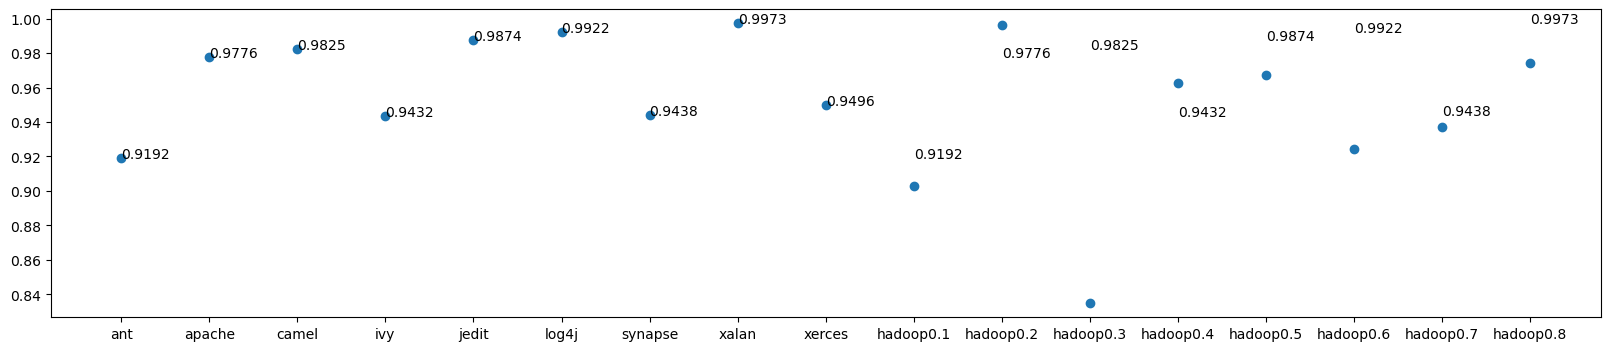
\includegraphics[width=\textwidth]{figures/overlap-F1.png}
    \caption{Overlap F1}
    \label{fig:overlap-f1-big}
\end{figure}

\begin{figure}[h!]
    \centering
    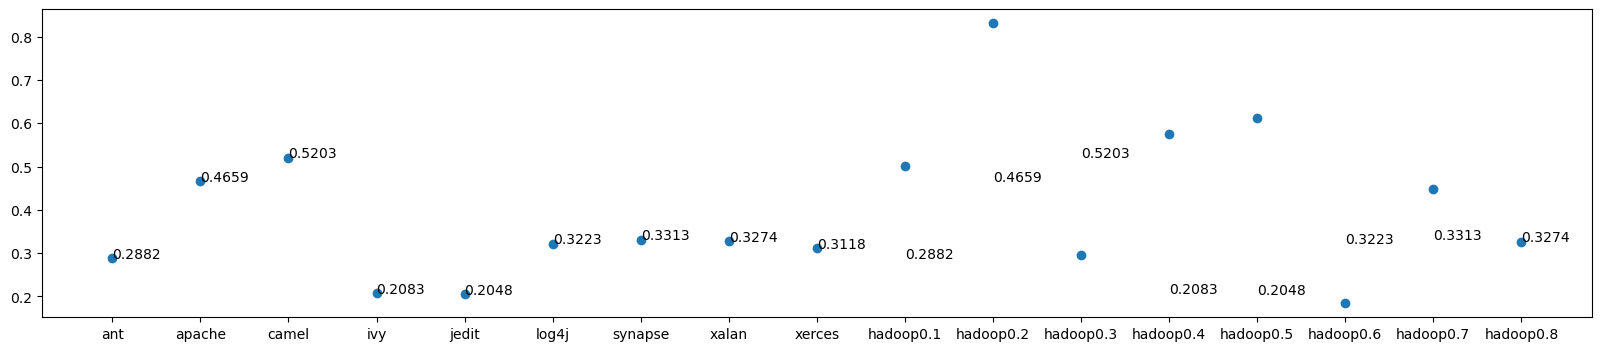
\includegraphics[width=\textwidth]{figures/overlap-F1v.png}
    \caption{Overlap F1v}
    \label{fig:overlap-f1v-big}
\end{figure}

\begin{figure}[h!]
    \centering
    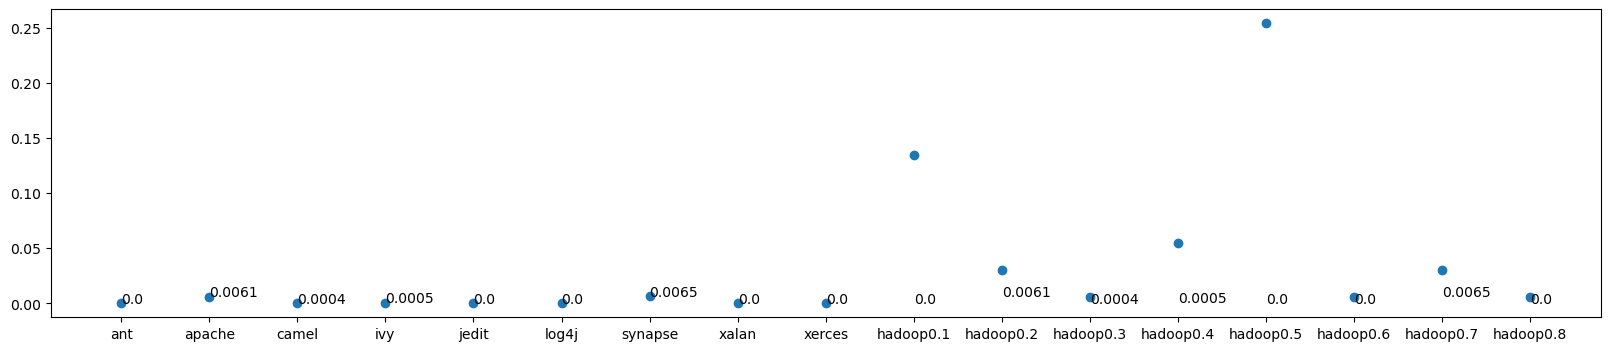
\includegraphics[width=\textwidth]{figures/overlap-F2.png}
    \caption{Overlap F2}
    \label{fig:overlap-f2-big}
\end{figure}

\begin{figure}[h!]
    \centering
    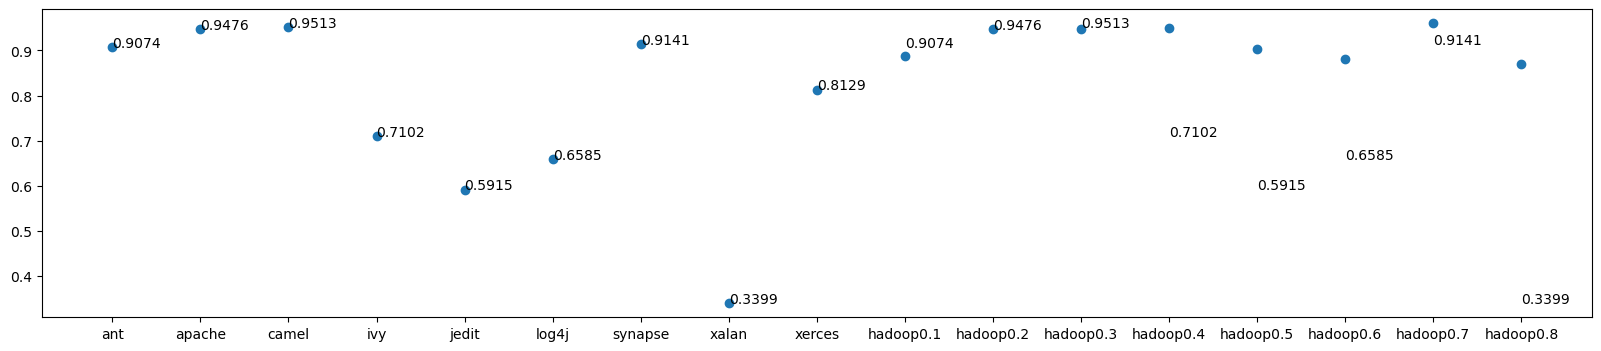
\includegraphics[width=\textwidth]{figures/overlap-F3.png}
    \caption{Overlap F3}
    \label{fig:overlap-f3-big}
\end{figure}
    
\begin{figure}[h!]
    \centering
    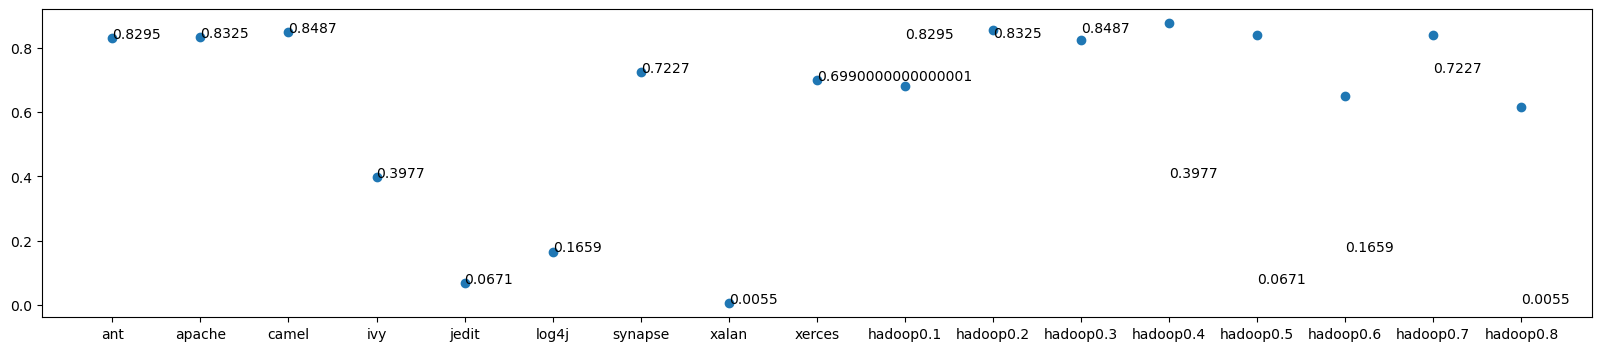
\includegraphics[width=\textwidth]{figures/overlap-F4.png}
    \caption{Overlap F4}
    \label{fig:overlap-f4-big}
\end{figure}

%%%%%%%%%%%%%%%%%%%%%%%%%%%%%%%%%%%%%%%%%%%%%%%%%%%%%%%%%%%%%%%%%%%%%%
% Neighborhood Metrics

\begin{figure}[h!]
    \centering
    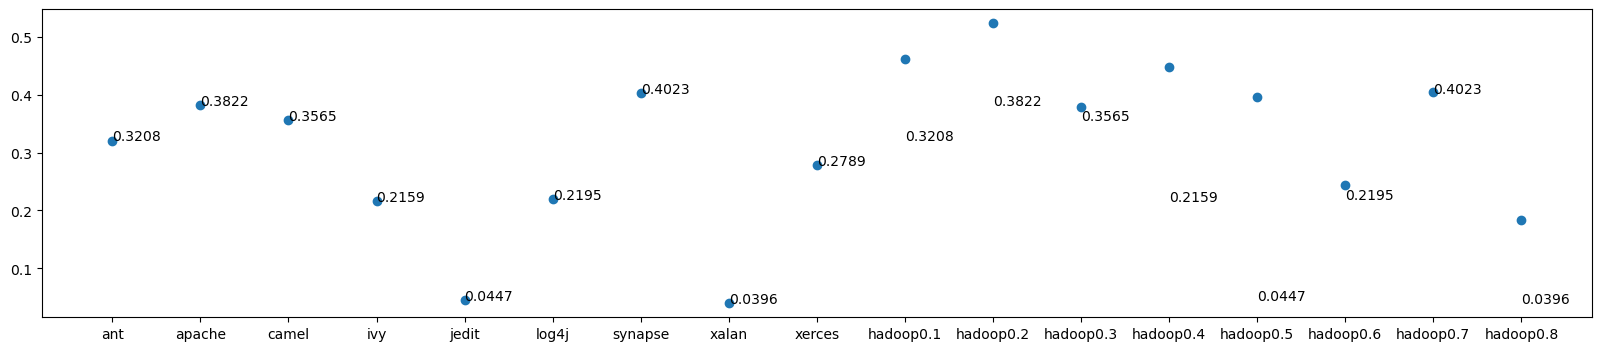
\includegraphics[width=\textwidth]{figures/neighborhood-N1.png}
    \caption{Neighborhood N1}
    \label{fig:neighborhood-n1-big}
\end{figure}

\begin{figure}[h!]
    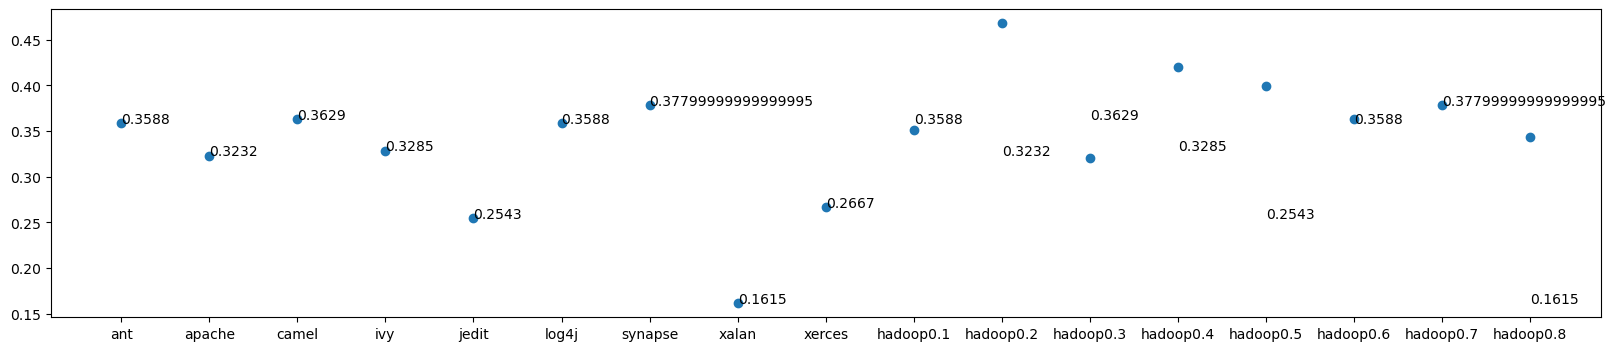
\includegraphics[width=\textwidth]{figures/neighborhood-N2.png}
    \caption{Neighborhood N2}
    \label{fig:neighborhood-n2-big}
\end{figure}

\begin{figure}[h!]
    \centering
    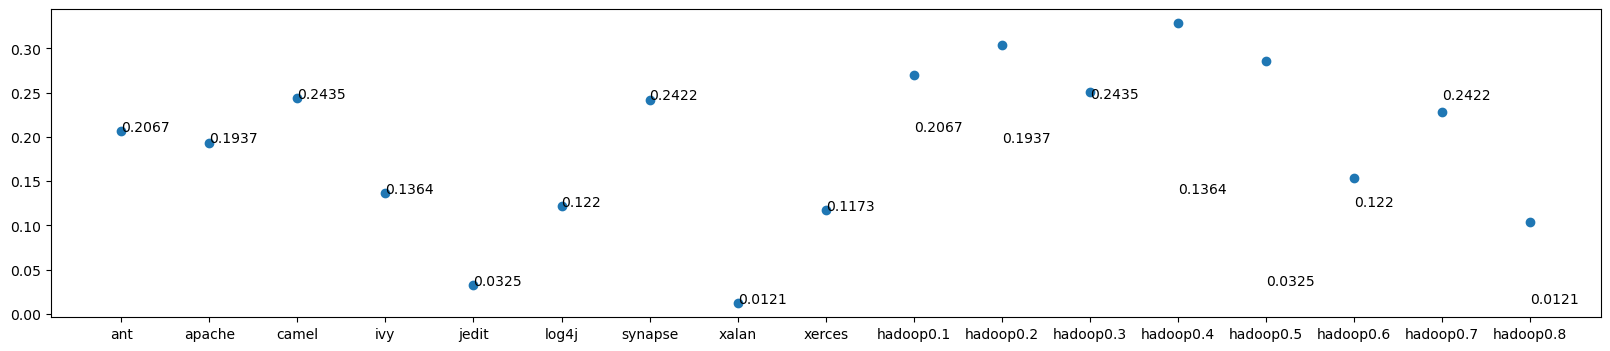
\includegraphics[width=\textwidth]{figures/neighborhood-N3.png}
    \caption{Neighborhood N3}
    \label{fig:neighborhood-n3-big}
\end{figure}

\begin{figure}[h!]
    \includegraphics[width=\textwidth]{figures/neighborhood-N4.png}
    \caption{Neighborhood N4}
    \label{fig:neighborhood-n4-big}
\end{figure}

\begin{figure}[h!]
    \includegraphics[width=\textwidth]{figures/neighborhood-T1.png}
    \caption{Neighborhood T1}
    \label{fig:neighborhood-t1-big}
\end{figure}

\begin{figure}[h!]
    \includegraphics[width=\textwidth]{figures/neighborhood-LSC.png}
    \caption{Neighborhood LSC}
    \label{fig:neighborhood-lsc-big}
\end{figure}

%%%%%%%%%%%%%%%%%%%%%%%%%%%%%%%%%%%%%%%%%%%%%%%%%%%%%%%%%%%%%%%%%%%%%%
% Linearity Metrics

\begin{figure}[h!]
    \includegraphics[width=\textwidth]{figures/linearity-L1.png}
    \caption{Linearity L1}
    \label{fig:linearity-l1-big}
\end{figure}

\begin{figure}[h!]
    \includegraphics[width=\textwidth]{figures/linearity-L2.png}
    \caption{Linearity L2}
    \label{fig:linearity-l2-big}
\end{figure}

\begin{figure}[h!]
    \includegraphics[width=\textwidth]{figures/linearity-L3.png}
    \caption{Linearity L3}
    \label{fig:linearity-l3-big}
\end{figure}

%%%%%%%%%%%%%%%%%%%%%%%%%%%%%%%%%%%%%%%%%%%%%%%%%%%%%%%%%%%%%%%%%%%%%%
% Dimensionality Metrics

\begin{figure}[h!]
    \includegraphics[width=\textwidth]{figures/dimensionality-T2.png}
    \caption{Dimensionality T2}
    \label{fig:dimensionality-t2-big}
\end{figure}

\begin{figure}[h!]
    \includegraphics[width=\textwidth]{figures/dimensionality-T3.png}
    \caption{Dimensionality T3}
    \label{fig:dimensionality-t3-big}
\end{figure}

%%%%%%%%%%%%%%%%%%%%%%%%%%%%%%%%%%%%%%%%%%%%%%%%%%%%%%%%%%%%%%%%%%%%%%
% Balance Metrics

\begin{figure}[h!]
    \centering
    \includegraphics[width=\linewidth]{figures/balance-C1.png}
    \caption{Balance C1}
    \label{fig:balance-c1-big}
\end{figure}

\begin{figure}[h!]
    \includegraphics[width=\linewidth]{figures/balance-C2.png}
    \caption{Balance C2}
    \label{fig:balance-c2-big}
\end{figure}

%%%%%%%%%%%%%%%%%%%%%%%%%%%%%%%%%%%%%%%%%%%%%%%%%%%%%%%%%%%%%%%%%%%%%%
% Network Metrics

\begin{figure}[h!]
    \includegraphics[width=\textwidth]{figures/network-Density.png}
    \caption{Network Density}
    \label{fig:network-density-big}
\end{figure}

\begin{figure}[h!]
    \includegraphics[width=\textwidth]{figures/network-ClsCoef.png}
    \caption{Network ClsCoef}
    \label{fig:network-clscoef-big}
\end{figure}

\begin{figure}[h!]
    \includegraphics[width=\textwidth]{figures/network-Hubs.png}
    \caption{Network Hubs}
    \label{fig:network-hubs-big}
\end{figure}

%%%%%%%%%%%%%%%%%%%%%%%%%%%%%%%%%%%%%%%%%%%%%%%%%%%%%%%%%%%%%%%%%%%%%%
% Correlation Metrics

\begin{figure}[h!]
    \includegraphics[width=\textwidth]{figures/correlation-C2.png}
    \caption{Correlation C2}
    \label{fig:correlation-c2-big}
\end{figure}

\begin{figure}[h!]
    \includegraphics[width=\textwidth]{figures/correlation-C3.png}
    \caption{Correlation C3}
    \label{fig:correlation-c3-big}
\end{figure}

\begin{figure}[h!]
    \includegraphics[width=\textwidth]{figures/correlation-C4.png}
    \caption{Correlation C4}
    \label{fig:correlation-c4-big}
\end{figure}

%%%%%%%%%%%%%%%%%%%%%%%%%%%%%%%%%%%%%%%%%%%%%%%%%%%%%%%%%%%%%%%%%%%%%%
% Smoothness Metrics

\begin{figure}[h!]
    \includegraphics[width=\textwidth]{figures/smoothness-S1.png}
    \caption{Smoothness S1}
    \label{fig:smoothness-s1-big}
\end{figure}

\begin{figure}[h!]
    \includegraphics[width=\textwidth]{figures/smoothness-S2.png}
    \caption{Smoothness S2}
    \label{fig:smoothness-s2-big}
\end{figure}

\begin{figure}[h!]
    \includegraphics[width=\textwidth]{figures/smoothness-S3.png}
    \caption{Smoothness S3}
    \label{fig:smoothness-s3-big}
\end{figure}

\begin{figure}[h!]
    \includegraphics[width=\textwidth]{figures/smoothness-S4.png}
    \caption{Smoothness S4}
    \label{fig:smoothness-s4-big}
\end{figure}


%
% END Appendices. Edit/modify all within this section
%%%%%%%%%%%%%%%%%%%%%%%%%%%%%%%%%%%%%%%%%%%%%%%%%%%%%%%%%%%%%%%%%%%%%%%%%%%

%%%%%%%%%%%%%%%%%%%%%%%%%%%%%%%%%%%%%%%%%%%%%%%%%%%%%%%%%%%%%%%%%%%%%%%%%%%
% Now start text and numbering for backmatter (just backpage in our
% case)
%%%%%%%%%%%%%%%%%%%%%%%%%%%%%%%%%%%%%%%%%%%%%%%%%%%%%%%%%%%%%%%%%%%%%%%%%%%
\backmatter                                       % DO NOT TOUCH THIS LINE!

%%%%%%%%%%%%%%%%%%%%%%%%%%%%%%%%%%%%%%%%%%%%%%%%%%%%%%%%%%%%%%%%%%%%%%%%%%%
% Just for TFGs at UAH right now, but kept here JIC anybody else wants
% to use it
%%%%%%%%%%%%%%%%%%%%%%%%%%%%%%%%%%%%%%%%%%%%%%%%%%%%%%%%%%%%%%%%%%%%%%%%%%%
%%%%%%%%%%%%%%%%%%%%%%%%%%%%%%%%%%%%%%%%%%%%%%%%%%%%%%%%%%%%%%%%%%%%%%%%%%%
%
% Generic template for TFC/TFM/TFG/Tesis
%
% $Id: backpage.tex,v 1.4 2014/01/08 22:56:05 macias Exp $
%
% By:
%  + Javier Mac�as-Guarasa. 
%    Departamento de Electr�nica
%    Universidad de Alcal�
%  + Roberto Barra-Chicote. 
%    Departamento de Ingenier�a Electr�nica
%    Universidad Polit�cnica de Madrid   
% 
% Based on original sources by Roberto Barra, Manuel Oca�a, Jes�s Nuevo,
% Pedro Revenga, Fernando Herr�nz and Noelia Hern�ndez. Thanks a lot to
% all of them, and to the many anonymous contributors found (thanks to
% google) that provided help in setting all this up.
%
% See also the additionalContributors.txt file to check the name of
% additional contributors to this work.
%
% If you think you can add pieces of relevant/useful examples,
% improvements, please contact us at (macias@depeca.uah.es)
%
% Copyleft 2013
%
%%%%%%%%%%%%%%%%%%%%%%%%%%%%%%%%%%%%%%%%%%%%%%%%%%%%%%%%%%%%%%%%%%%%%%%%%%%

%%%%%%%%%%%%%%%%%%%%%%%%%%%%%%%%%%%%%%%%%%%%%%%%%%%%%%%%%%%%%%%%%%%%%%%%%%%
% Right now (november 2013), it's only defined for TFGs at UAH
%%%%%%%%%%%%%%%%%%%%%%%%%%%%%%%%%%%%%%%%%%%%%%%%%%%%%%%%%%%%%%%%%%%%%%%%%%%

\ifthenelse{\equal{\mybookworktype}{TFG}}
{
  %%%%%%%%%%%%%%%%%%%%%%%%%%%%%%%%%%%%%%%%%%%%%%%%%%%%%%%%%%%%%%%%%%%%%%%%%%%
%
% Generic template for TFC/TFM/TFG/Tesis
%
% $Id: backpage-tfg-uah.tex,v 1.9 2014/12/09 11:55:53 macias Exp $
%
% By:
%  + Javier Mac�as-Guarasa. 
%    Departamento de Electr�nica
%    Universidad de Alcal�
%  + Roberto Barra-Chicote. 
%    Departamento de Ingenier�a Electr�nica
%    Universidad Polit�cnica de Madrid   
% 
% Based on original sources by Roberto Barra, Manuel Oca�a, Jes�s Nuevo,
% Pedro Revenga, Fernando Herr�nz and Noelia Hern�ndez. Thanks a lot to
% all of them, and to the many anonymous contributors found (thanks to
% google) that provided help in setting all this up.
%
% See also the additionalContributors.txt file to check the name of
% additional contributors to this work.
%
% If you think you can add pieces of relevant/useful examples,
% improvements, please contact us at (macias@depeca.uah.es)
%
% Copyleft 2013
%
%%%%%%%%%%%%%%%%%%%%%%%%%%%%%%%%%%%%%%%%%%%%%%%%%%%%%%%%%%%%%%%%%%%%%%%%%%%

% This is a trick to avoid the header to be shown. There must be a
% better way...
\chapter*{ }
\thispagestyle{empty}

\cleartoleftpage
\thispagestyle{empty}

% To add background watermark, defined in config/preamble.tex
\BgThispage

% Nice example of tikz
% \begin{tikzpicture}[remember picture,overlay]
%   \node [xshift=1cm,yshift=1cm] at (current page.south west)
%   [text width=7cm,fill=red,red!20,rounded corners,above right]
%   {
%     This is an absolutely positioned text in the
%     lower left corner. No shipout-hackery is used.
%   };
% \end{tikzpicture}

\begin{tikzpicture}[remember picture,overlay]
    \node[yshift=-5cm] at (current page.north west)
      {
        \begin{tikzpicture}[remember picture, overlay]
          \draw[fill=headingPortadaTFG,headingPortadaTFG] (0,0) rectangle (\paperwidth,5cm);

          \node [yshift=3cm, xshift=0.5\paperwidth, font=\Huge, text centered, midway] {\color{textoHeadingPortadaTFG}\mybookuniversity};
          \node [yshift=2cm, xshift=0.5\paperwidth, font=\Huge, text centered, midway] {\color{textoHeadingPortadaTFG}\mybookschool};

        \end{tikzpicture}
      };
   \end{tikzpicture}


\large
\vspace{20cm}
\begin{center}
  
  \centerline{\includegraphics[height=2.5cm]{uah/01_logo-vA_pant293.pdf}}

\end{center}



%%% Local Variables:
%%% TeX-master: "../book"
%%% End:



}
{

}

%%% Local Variables:
%%% TeX-master: "../book"
%%% End:


                    % EDIT this file if
                                              % required, or comment it out

\end{document}

